
%%%%%%%%%%%%%%%%%%%%%%%%%%%%%%%%%%%%%%%%%%%%%%%%%%%%%%%%%%%%%%%%%%%%%%%%%%%%%%%%
%  
%-------------------------------------------------------------------------------
%  
%-------------------------------------------------------------------------------
%  28-06-2012
%-------------------------------------------------------------------------------

% 
%%%%%%%%%%%%%%%%%%%%%%%%%%%%%%%%%%%%%%%%%%%%%%%%%%%%%%%%%%%%%%%%%%%%%%%%%%%%%%%%
\makeatletter\def\input@path{{booktex/}}\makeatother
%-------------------------------------------------------------------------------
% Chargement de la class FramateX
\documentclass{FramateX}
%-------------------------------------------------------------------------------

%-----------------------------------------------------------------------
% Hyperref, Liens et autres details
\usepackage{hyperref}
\hypersetup{colorlinks=true,citecolor=black,filecolor=black,linkcolor=black,urlcolor=black,bookmarks=false}
%-----------------------------------------------------------------------

% Gestion de la langue
\usepackage[frenchb]{babel}
%-------------------------------------------------------------------------------
% Gestion des dimensions
\usepackage[paperwidth=148mm,paperheight=210mm,twoside]{geometry}
\geometry{inner=25mm,outer=20mm,top=20mm,bottom=20mm}
%-------------------------------------------------------------------------------
% Gestion des entetes, bas de page, section, chapitre....
\usepackage{FramateXentete}

%---------------------------------------
% Ornements

%--------------------------Pour inserer du code -------------------
\usepackage{verbatim}
\usepackage{listings}

%%%% Pour configurer listing afin d'obtenir du code java
\definecolor{javared}{rgb}{0.6,0,0} % for strings
\definecolor{javagreen}{rgb}{0.25,0.5,0.35} % comments
\definecolor{javapurple}{rgb}{0.5,0,0.35} % keywords
\definecolor{javadocblue}{rgb}{0.25,0.35,0.75} % javadoc

\lstset{language=Java,
basicstyle=\sffamily\footnotesize,
keywordstyle=\color{javapurple}\bfseries,
stringstyle=\color{javared},
commentstyle=\color{javagreen},
morecomment=[s][\color{javadocblue}]{/**}{*/},
xleftmargin=20pt,
xrightmargin=20pt,
numbers=left,
numberstyle=\tiny\color{black}, %Numeros de ligne
stepnumber=1, % le pas des numeros de ligne
numbersep=10pt,
breaklines=true,
tabsize=4,
%frame=single,
showspaces=false,
showstringspaces=false
inputencoding=utf8, %put1 d'utf8 dans listing
extendedchars=true, %put1 d'utf8 dans listing
literate={à}{{\`a}}1 {é}{{\'e}}1 {è}{{\`e}}1 {ê}{{\^e}}1 {â}{{\^a}}1 {î}{{\^i}}1 {ê}{{\^e}}1 {É}{{\'E}}1 {À}{{\`A}}1 {«}{{\og}}1 {»}{{\fg{}}}1 {ô}{{\^o}}1 {ù}{{\`u}}1 {û}{{\^u}}1 {ç}{{\c{c}}}1 {Ç}{{\c{C}}}1, %put1 d'utf8 dans listing
}
%%%%%%%%%%%%%%%%%%%%%


%%%%%% pour reconfigurer txttt dans le texte
\renewcommand{\texttt}[1]{\begin{sffamily}{#1}\end{sffamily}}



% remize à zéro du compteur des chapitres pour une nouvelle partie
\makeatletter 
\@addtoreset{chapter}{part} 
\makeatother

\usepackage[toc,page]{appendix} 

\selectlanguage{francais}
\frenchspacing



%------------------ POUR ASSURER PLEINE COMPATIBILITE avec les imprimeur : PDF 1.3
% (et eviter les effets de calques produits avec pdf 1.4)
% il faut compiler avec pdflatex mais en version 3
\pdfminorversion=3


%-------------------------------------------------------------------------------
% fin du préambule
%-------------------------------------------------------------------------------
\begin{document}
\sloppy % Ce sloppy sera actif jusquau end{document}
\renewcommand{\figurename}{F\textsc{igure} }
\renewcommand{\tablename}{T\textsc{able} }

\def\appendixpage{\vspace*{8cm}
\begin{center}
\Huge\textbf{Annexes}
\end{center}
}
\def\appendixname{Annexe}



\frontmatter                        

            
\begin{titlepage}
\vspace*{\stretch{0.2}}
\noindent\rule{\linewidth}{1pt}
\begin{center}\LARGE{Marijn Haverbeke}\end{center}
\noindent\rule{\linewidth}{1pt}
\vspace*{\stretch{2}}
\begin{center}\Huge{Eloquent Javascript}\end{center}
\vspace*{\stretch{0.2}}
\begin{center}\LARGE{blabla}\end{center}
\vspace*{\stretch{2}}
\begin{center}

\begin{figure}[!ht]
\begin{center}  
\includegraphics[width=70mm,height=20mm]{img/Logo_framabook_grand.png}  \end{center}
\end{figure}

\end{center}
\vspace*{\stretch{4}}
\begin{center}
\noindent\rule{\linewidth/2}{1pt} \\
\end{center}
\begin{center}Publié sous licence\end{center}
\begin{center}CC By 3.0\end{center}
\newpage 
\begin{flushleft}Framasoft a été créé en novembre 2001 par Alexis Kauffmann. En janvier 2004 une association éponyme a vu le jour pour soutenir le développement du réseau. Pour plus d’information sur Framasoft, consulter http://www.framasoft.net.\end{flushleft}
\begin{flushleft}Se démarquant de l’édition classique, les Framabooks sont dits «~livres libres~» parce qu’ils sont placés sous une licence qui permet au lecteur de disposer des mêmes libertés qu’un utilisateur de logiciels libres. Les Framabooks s’inscrivent dans cette culture des biens communs qui, à l’instar de Wikipédia, favorise la création, le partage, la diffusion et l’appropriation collective de la connaissance.\end{flushleft}
\begin{flushleft}Le projet Framabook est coordonné par Christophe Masutti. Pour plus d’information, consultez http://framabook.org.\end{flushleft}
\begin{center}\rule{100mm}{1pt}\end{center}\bigskip{}

\bigskip

\begin{small}
\noindent Copyright 2012~: Marijn Haverbeke, Framasoft (coll. Framabook)\\
\textit{Eloquent Javascript} est placé sous~: Creative Commons By (3.0).

\noindent ISBN~: 978-1-4716-1234-3 \\
Prix~: xx euros \\
Dépôt légal~: 2012, LULU.COM \\
Pingouins~: LL de Mars, Licence Art Libre \\
Couverture~: création par ?, Licence CC By \\
Mise en page avec \LaTeX  \\
\end{small}



\end{titlepage}

                        
                        
                       
                        
% -------------------------------------------------------------------------
%
\cleardoublepage
\phantomsection

\chapter*{Remerciements}
\addcontentsline{toc}{chapter}{Remerciements}
%
% -------------------------------------------------------------------------

Mes plus sincères remerciements à ...........

                        
                        
% -------------------------------------------------------------------------
%

\cleardoublepage
\phantomsection
\chapter*{Préface}
\addcontentsline{toc}{chapter}{Préface}
%
% -------------------------------------------------------------------------

                    

Ceci est le texte de la préface



% -------------------------------------------------------------------------
%
\cleardoublepage
\phantomsection
\chapter*{Quelques acronymes et abréviations utilisés}
\addcontentsline{toc}{chapter}{Quelques acronymes et abréviations utilisés}
%
% -------------------------------------------------------------------------

                    

Liste descriptive si besoin

                        
                        
% -------------------------------------------------------------------------
%
\cleardoublepage
\phantomsection
\chapter*{Introduction}
\addcontentsline{toc}{chapter}{Introduction}


Lorsque les premiers ordinateurs personnels sont apparus, la plupart
d'entre eux étaient fournis avec un langage de programmation simple,
généralement une variante de BASIC. Les interactions avec l'ordinateur
étaient fortement liées à ce langage, et tout utilisateur d'un
ordinateur devait dès lors y goûter, qu'il le veuille ou non. À présent
que les ordinateurs sont devenus nombreux et bon marché, l'utilisateur
moyen se contente la plupart du temps de ce qu'il peut faire en cliquant
avec la souris. Pour nombre d'entre eux, cela fonctionne très bien. Mais
pour ceux d'entre nous qui ont une inclination naturelle au bricolage
technique, la disparition de la programmation dans l'usage quotidien
d'un ordinateur représente une forme de barrière.

Heureusement, avec l'évolution du World Wide Web, il se trouve que
chaque ordinateur équipé d'un navigateur web moderne a également un
environnement pour programmer en JavaScript. Il est gardé bien caché car
il est dans l'air du temps de ne pas ennuyer l'utilisateur avec des
détails techniques, mais une page web peut le rendre accessible et
l'utiliser comme une plateforme pour apprendre à programmer.

C'est ce que ce livre (ou hyper-livre) essaie de faire.

\begin{center}\ding{67}\end{center}

\begin{quote}
Je n'ai pas pour but d'éclairer ceux qui ne sont pas désireux
d'apprendre, ni éveiller ceux qui ne sont pas soucieux de donner une
explication eux-mêmes. Si je leur ai montré un angle du carré et qu'ils
ne peuvent pas revenir à moi avec les trois autres, je ne devrais pas
revenir sur le premier angle.\\\\--- Confucius
\end{quote}
Au-delà des explications qu'il donne sur le JavaScript, ce livre
s'efforce d'initier aux principes fondamentaux de la programmation.
Programmer s'avère être un exercice difficile. Les règles de base sont
la plupart du temps simples et claires. Cependant, même des programmes
construits suivant ces règles de base, tendent à devenir suffisamment
élaborés pour générer leurs propres règles et leur propre complexité.
Voilà pourquoi la programmation est rarement simple et prévisible. Comme
le dit Donald Knuth, que l'on peut considérer comme un des pères
fondateurs dans ce domaine, c'est un \emph{art}.

Pour tirer quelque chose de ce livre, il est indispensable de faire plus
que de le lire passivement. Essayez de garder l'esprit affûté,
efforcez-vous de résoudre les exercices, et n'allez plus loin que
lorsque vous êtes certain d'avoir bien assimilé les étapes précédentes.

\begin{center}\ding{67}\end{center}

\begin{quote}
Le programmeur en informatique est un créateur d'univers dont il est
seul responsable. Des univers d'une complexité potentiellement illimitée
peuvent être créés sous forme de programmes informatiques.\\\\-- Joseph
Weizenbaum, \emph{La puissance de l'ordinateur et la raison humaine}
\end{quote}
Un programme, c'est beaucoup de choses. C'est un bout de texte tapé par
un programmeur, c'est la force directrice qui indique à l'ordinateur ce
qu'il doit faire, c'est un ensemble de données dans la mémoire de
l'ordinateur, et pourtant il contrôle les actions accomplies dans cette
même mémoire. Les analogies qui comparent les programmes à des objets
qui nous sont familiers ont tendance à tourner court alors que celle
d'une machine est, de manière superficielle, mieux adaptée. Les roues et
les engrenages d'une montre mécanique sont ingénieusement agencés et
coordonnés, et si l'horloger connaît son affaire, la montre donnera
l'heure pendant des années. Les parties d'un programme sont de même
étroitement solidaires et si le programmeur sait ce qu'il fait, son
programme fonctionnera sans plantage.

Un ordinateur est une machine conçue pour héberger ce genre de machines
immatérielles. Les ordinateurs eux-mêmes ne peuvent qu'exécuter
stupidement des choses simples. S'ils sont très utiles, c'est parce
qu'ils peuvent faire ces choses à une vitesse incroyable. Un programme
peut, en combinant un grand nombre de ces actions simples, accomplir des
tâches très complexes.

Pour beaucoup d'entre nous, écrire des programmes informatiques est un
jeu fascinant. Un programme est une construction de l'esprit. Il ne
coûte rien à élaborer, il ne pèse rien et se développe facilement sous
nos mains. Si nous nous laissons aller, sa taille et sa complexité vont
prendre des proportions démesurées, au point d'échapper au contrôle même
de celui qui l'a créé. C'est le principal problème de la programmation.
C'est la raison pour laquelle beaucoup de logiciels aujourd'hui
finissent par planter, échouer et tout saloper.

Quand un programme fonctionne, c'est beau. L'art de la programmation est
l'art de contrôler la complexité. Un programme de grande qualité est
discret et apparaît simple malgré sa complexité.

\begin{center}\ding{67}\end{center}

Aujourd'hui, beaucoup de programmeurs croient que cette complexité est
plus facile à gérer en utilisant seulement un petit jeu de techniques
bien comprises dans leurs programmes. Ils ont élaboré des règles
strictes concernant la forme que devraient adopter les programmes, et
les plus zélés d'entre eux dénonceront ceux qui enfreignent ces règles
comme de \emph{mauvais} programmeurs.

Quelle hostilité envers la richesse de la programmation ! Essayer de la
réduire à quelque chose de direct et de prévisible, jeter l'opprobre sur
tous les programmes bizarres et magnifiques. Le champ des techniques de
programmation est gigantesque, fascinant par sa diversité et encore
largement inexploré. Il est certainement bourré de chausse-trappes et de
pièges à loups, menaçant de faire commettre au programmeur inexpérimenté
toute sorte d'affreuses erreurs. Cela signifie seulement que vous devez
procéder avec prudence et garder votre sang-froid. En apprenant, vous
rencontrerez toujours de nouveaux défis, de nouveaux territoires à
explorer. Le programmeur qui refuse l'exploration va sûrement végéter,
ne plus trouver ça drôle, perdre le désir de programmer (et devenir chef
de projet).

En ce qui me concerne, le critère décisif pour évaluer un programme est
: «~Est-il correct ?~». L'efficacité, la clarté et la taille sont
également importantes, mais pouvoir peser avec exactitude le poids de
l'un et le poids de l'autre est toujours une question d'opinion, une
opinion que doit se faire chaque programmeur. Les règles générales sont
utiles, mais on ne devrait jamais avoir peur de les transgresser.

\begin{center}\ding{67}\end{center}

Au début de l'informatique, lorsqu'elle venait de naître, il n'existait
pas de langage de programmation. Les programmes ressemblaient à ceci :

\begin{lstlisting}
00110001 00000000 00000000
00110001 00000001 00000001
00110011 00000001 00000010
01010001 00001011 00000010
00100010 00000010 00001000
01000011 00000001 00000000
01000001 00000001 00000001
00010000 00000010 00000000
01100010 00000000 00000000
\end{lstlisting}

Il s'agit d'un programme qui fait la somme des nombres de 1 à 10 et
donne le résultat (1 + 2 + \ldots{} + 10 = 55). Il pourrait tourner sur
l'ordinateur le plus simple. Pour programmer les premiers ordinateurs,
il était nécessaire de disposer de grandes séries d'interrupteurs dans
la bonne position, ou de perforer des trous dans des cartes et les faire
avaler à la machine. Vous imaginez facilement à quel point la procédure
était fastidieuse et sujette à erreurs. Écrire ne serait-ce qu'un
programme simple exigeait beaucoup d'intelligence et de discipline, les
programmes complexes étaient carrément hors d'atteinte.

Bien entendu, saisir à la main des masques de bits (c'est ainsi qu'on
appelle en général les suites de 1 et de 0 ci-dessus) donnait au
programmeur l'impression d'être un puissant sorcier. Cela ne peut pas
compter pour du beurre en ce qui concerne la satisfaction
professionnelle.

Chaque ligne de programme contient une instruction unique. On pourrait
l'exprimer en français sous cette forme :

\begin{enumerate}
\item
  Stocker le nombre 0 à l'adresse mémoire 0
\item
  Stocker le nombre 1 à l'adresse mémoire 1
\item
  Stocker la valeur de l'adresse mémoire 1 dans l'adresse mémoire 2
\item
  Soustraire 11 de la valeur stockée à l'adresse mémoire 2
\item
  Si la valeur à l'adresse mémoire 2 est le nombre 0, continuer à
  l'instruction 9
\item
  Ajouter la valeur de l'adresse mémoire 1 à l'adresse mémoire 0
\item
  Ajouter le nombre 1 à la valeur de l'adresse mémoire 1
\item
  Continuer avec l'instruction 3
\item
  Donner la valeur de l'adresse mémoire 0
\end{enumerate}
Alors que c'est déjà plus lisible que la soupe binaire, cela reste assez
désagréable. Il pourrait être utile d'utiliser des noms au lieu de
nombres pour les instructions et les adresses mémoire :

\begin{lstlisting}
 Mettre 0 à 'total'
 Mettre 1 à 'compteur'
[boucle]
 Mettre 'compteur' à 'comparaison'
 Soustraire 11 à 'comparaison'
 Si 'comparaison' est zero, continuer à [fin]
 Ajouter 'compteur' à 'total'
 Ajouter 1 à 'compteur'
 Continuer à [boucle]
[fin]
 Afficher 'total'
\end{lstlisting}
À partir de là il n'est pas trop difficile de deviner comment fonctionne
le programme. Qu'en dites-vous ? Les deux premières lignes donnent leur
valeur initiale aux adresses mémoire : \texttt{total} sera utilisé pour
calculer le résultat du programme et \texttt{compteur} conserve le
nombre courant. Les lignes qui utilisent \texttt{comparaison} sont
probablement les plus bizarres. Ce que le programme cherche à savoir
c'est si \texttt{compteur} est égal à 11, de manière à savoir s'il doit
interrompre le calcul. Comme la machine est très rudimentaire, il peut
seulement tester si un nombre est zéro, et prend une décision (sauter)
basée sur ce critère. il utilise donc l'adresse mémoire nommée
\texttt{comparaison} pour calculer la valeur de \texttt{compteur - 11},
et décide suivant la valeur obtenue. Les deux lignes suivantes ajoutent
la valeur de \texttt{compteur} au résultat, et l'incrémentent
\texttt{compteur} d'une unité à chaque fois que le programme a décidé
qu'il n'avait pas encore atteint 11.

Voici maintenant le même programme en JavaScript :

\begin{lstlisting}
var total = 0, compteur = 1;
while (compteur <= 10) {
  total += compteur;
  compteur += 1;
}
print(total);
\end{lstlisting}
C'est encore un peu mieux pour nous. Le plus important est qu'il n'y a
plus besoin de préciser la façon dont nous voulons que le programme
fasse un bond par-ci par-là. Le mot magique \texttt{while} s'en occupe.
Le programme continue à exécuter les lignes ci-dessous tant que la
condition qu'on lui a donnée est satisfaite :
\texttt{compteur \textless{}= 10}, ce qui veut dire tant que «
\texttt{compteur} est inférieur ou égal à \texttt{10}~». Apparemment, il
n'y a plus besoin de créer une valeur temporaire et de la comparer à
zéro. C'était un petit détail stupide, et le pouvoir des langages de
programmation est justement qu'ils règlent pour nous ce genre de choses
accessoires.

(NdT : \texttt{while} n'est pas traduit car c'est un mot du langage
JavaScript, \texttt{print} non plus, c'est un des différents mots que
vous retrouverez souvent en anglais dans la littérature ou dans d'autres
programmes.)

Finalement, voici à quoi pourrait ressembler le programme si nous nous
étions arrangés pour que les opérations \texttt{serie} et \texttt{somme}
soient disponibles, la première créant une collection de nombres dans
une série tandis que la seconde calcule la somme d'une série de nombres
:

\begin{lstlisting}
print(somme(serie(1, 10)));
\end{lstlisting}
La morale de cette histoire est donc que le même programme peut être
exprimé de façon brève ou longue, lisible ou illisible. La première
version du programme était extrêmement obscure, tandis que la dernière
est quasiment du français : \texttt{print} (afficher) la \texttt{somme}
de la \texttt{serie} des nombres de \texttt{1} à \texttt{10}. Nous
verrons par la suite dans d'autres chapitres comment construire des
choses telles que \texttt{somme} et \texttt{serie}.

Un bon langage de programmation aide le programmeur en lui fournissant
une manière plus abstraite de s'exprimer. Il masque les détails
inintéressants, procure des composants de base pratiques (comme la
construction \texttt{while}) et, la plupart du temps, permet au
programmeur d'ajouter lui-même de telles briques (comme les opérations
\texttt{somme} et \texttt{serie}).

\begin{center}\ding{67}\end{center}

JavaScript est le langage qui est, actuellement, le plus utilisé pour
faire toutes sortes de choses géniales et horribles avec des pages sur
le World Wide Web.
\href{http://steve-yegge.blogspot.com/2007/02/next-big-language.html}{Certains}
prétendent que la prochaine version de JavaScript en fera un langage de
référence pour d'autres tâches également. J'ignore si cela va se
produire, mais si vous êtes intéressé par la programmation, JavaScript
est sans aucun doute un langage utile à apprendre. Même si en fin de
compte vous ne faites pas tellement de programmation web, les programmes
hallucinants que je vais vous montrer dans cet ouvrage resteront
toujours en vous, à vous hanter et à influencer les programmes que vous
écrirez dans d'autres langages.

Certains vous diront des choses \emph{terribles} à propos de JavaScript.
Beaucoup de ces reproches sont fondés. La première fois que j'ai dû
écrire quelque chose en JavaScript, j'ai rapidement méprisé ce langage.
Il acceptait à peu près tout ce que je tapais, mais l'interprétait d'une
façon complètement différente de celle que je voulais. Cela venait
surtout du fait que je n'avais aucune idée de ce que je faisais, mais il
y a aussi un véritable problème ici : JavaScript est absurdement laxiste
dans ce qu'il permet. L'idée derrière cette conception était de rendre
la programmation en JavaScript plus facile pour les débutants. En
réalité, il rend surtout plus difficile la recherche des problèmes dans
vos programmes, parce que le système ne vous les montrera pas.

Toutefois, la souplesse de ce langage est aussi un avantage. Elle laisse
la place à de nombreuses techniques que les langages de programmation
plus rigides ne permettent pas, et on peut l'utiliser pour compenser
certains défauts de JavaScript. Après l'avoir étudié correctement et
avoir travaillé avec un certain temps, j'ai vraiment appris à
\emph{aimer} ce langage.

\begin{center}\ding{67}\end{center}

Contrairement à ce que son nom suggère, JavaScript a très peu à voir
avec le langage de programmation nommé Java. Le nom similaire a été
inspiré par des considérations commerciales plutôt que rationnelles. En
1995, quand le JavaScript a été lancé par Netscape, le langage Java
était promu partout et gagnait en popularité. Apparemment, quelqu'un a
dû penser que c'était une bonne idée d'essayer de surfer sur la mode du
moment. Nous voilà aujourd'hui coincé avec ce nom.

Il existe un langage associé au JavaScript et qui s'appelle ECMAScript.
Quand les navigateurs autres que Netscape ont commencé à prendre en
charge le JavaScript, ou quelque chose du même genre, on a écrit une
documentation pour décrire avec précision comment le langage en question
devait fonctionner. On l'a appelé ECMAScript, d'après le nom de
l'organisation qui l'a standardisé.

ECMAScript décrit un langage de programmation à usage général, mais ne
dit rien sur l'intégration de ce langage dans un navigateur internet. Le
JavaScript c'est ECMAScript plus des outils supplémentaires pour gérer
les pages web et les fenêtres de navigation.

Quelques autres logiciels utilisent le langage décrit dans le document
ECMAScript. Plus important, le langage ActionScript utilisé par Flash
est basé sur ECMAScript (bien qu'il ne suive pas précisément le
standard). Flash est un système utilisé pour ajouter des trucs qui
bougent et font du bruit sur les pages web. Ça ne vous fera pas de mal
de connaître JavaScript si vous devez un jour apprendre à faire des
animations en Flash.

JavaScript continue d'évoluer. Depuis la sortie de cet ouvrage,
ECMAScript 5 est sorti, il est compatible avec la version décrite ici,
mais y ajoute, en tant que méthodes natives, quelques fonctionnalités
que nous écrirons nous-même. La dernière génération de navigateurs
fournit cette version augmentée de JavaScript. En 2011, «~ECMAScript
harmony~», une extension plus radicale du langage, est en cours de
standardisation. Vous ne devriez pas trop craindre que ces nouvelles
versions rendent obsolètes ce que vous apprenez dans ce livre. Il ne
s'agira que d'une extension du langage dont nous disposons actuellement,
donc pratiquement tout ce qui est écrit dans ce livre restera valide.

\begin{center}\ding{67}\end{center}

La plupart des chapitres de ce livre contiennent une quantité non
négligeable de code\footnote{Le «~Code~» est la substance dont sont composés les programmes. Chaque morceau de programme, que ce soit une ligne unique ou tout un ensemble, peut être appelé «~code~».}. D'après mon expérience, lire
et écrire du code est une part importante de l'apprentissage de la
programmation. Essayez de ne pas seulement jeter un œil sur ces exemples
mais lisez-les vraiment attentivement et comprenez-les. Cela peut être
long et déroutant au début, mais vous prendrez rapidement le coup. Il en
va de même concernant les exercices. N'estimez pas les comprendre avant
d'avoir effectivement écrit une solution qui fonctionne.

Le fonctionnement même du Web fait qu'il est toujours possible
d'examiner les programmes JavaScript que les gens utilisent dans leurs
pages web. Cela peut être un bon moyen d'apprendre comment certaines
choses sont réalisées. Étant donné que la plupart des programmeurs web
ne sont pas des programmeurs «~professionnels~», ou qu'ils ne
considèrent pas la programmation JavaScript comme suffisamment
intéressante pour en faire convenablement l'apprentissage, beaucoup du
code que vous pourrez trouver ainsi sera de \emph{très} mauvaise
qualité. Quand vous apprenez à partir de code laid et incorrect, la
laideur et la confusion se propagent dans votre propre code ; faites
donc très attention de qui vous prenez vos leçons.

\begin{center}\ding{67}\end{center}

Pour vous permettre d'essayer les programmes, aussi bien les exemples
que le code que vous écrirez vous-même, ce livre utilise ce que l'on
appelle une console. Si vous utilisez un navigateur graphique moderne
(Internet Explorer version 6 ou supérieur, Firefox 1.5 ou supérieur,
Opera 9 ou supérieur, Safari 3 ou supérieur), les pages de ce livre vont
afficher une barre bleuâtre en bas de votre écran. Vous pouvez ouvrir la
console en cliquant sur la petite flèche à l'extrémité droite de cette
barre (notez qu'il ne s'agit pas de la console intégrée de votre
navigateur).

La console contient trois éléments importants. Il y a une fenêtre de
sortie, qui est utilisée pour montrer les messages d'erreurs et les
choses qu'affichent les programmes. Sous celle-ci se trouve une ligne où
vous pouvez saisir un bout de JavaScript. Essayez de saisir un nombre et
appuyez sur la touche Entrée pour lancer ce que vous avez tapé. Si le
texte que vous avez saisi a produit quelque chose de sensé, cela sera
affiché dans la fenêtre de sortie. Maintenant, essayez de taper
\texttt{mauvais!}, et appuyez à nouveau sur Entrée. La fenêtre de sortie
va afficher un message d'erreur. Vous pouvez utiliser les touches flèche
vers le haut et flèche vers le bas pour revenir aux commandes que vous
avez saisies précédemment.

Pour les bouts de code plus importants, ceux qui s'étendent sur
plusieurs lignes et que vous voulez conserver un peu, la zone de droite
peut être utilisée. Le bouton «~Lancer~» est utilisé pour exécuter les
programmes écrits dans cette zone. Il est possible d'avoir plusieurs
programmes ouverts en même temps. Utilisez le bouton «~Nouveau~» pour
ouvrir un nouveau tampon vide. Quand il y a plus d'un programme ouvert,
le menu après le bouton «~Lancer~» peut être utilisé pour choisir lequel
est affiché. Le bouton «~Fermer~», comme vous pouvez vous en douter,
ferme un programme.

Il y a toujours un petit bouton avec une flèche dans le coin supérieur
droit des programmes d'exemple de ce livre, qui peut être utilisé pour
les lancer. L'exemple que nous avons vu auparavant ressemblait à ceci :

\begin{lstlisting}
var total = 0, compteur = 1;
while (compteur <= 10) {
  total += compteur;
  compteur += 1;
}
print(total);
\end{lstlisting}
Lancez-le en cliquant sur la flèche. Il y a aussi un autre bouton qui
sert à charger le programme dans la console. N'hésitez pas à le modifier
et à essayer le résultat. Le pire qu'il puisse arriver est que vous
créiez une boucle sans fin. Une boucle infinie est ce que vous obtenez
lorsque la condition d'un \texttt{while} ne devient jamais fausse, par
exemple si vous choisissez d'ajouter \texttt{0} au lieu de \texttt{1} à
la variable compteur. Alors le programme va tourner pour toujours.

Heureusement, les navigateurs gardent un œil sur les programmes qu'ils
font tourner. Lorsque l'un d'eux prend un délai démesuré pour se
terminer, ils vous demandent si vous voulez l'interrompre.

\begin{center}\ding{67}\end{center}

Dans certains chapitres à venir, nous créerons des programmes d'exemple
qui seront constitués de multiples blocs de code. Souvent, vous devrez
lancer chacun d'eux pour faire fonctionner le programme. Comme vous
l'avez peut-être remarqué, la flèche d'un bloc de code devient violette
lorsque le bloc a été exécuté. Lorsque vous lisez un chapitre, essayez
de lancer chaque bloc de code que vous rencontrez, particulièrement ceux
qui «~définissent~» quelque chose de nouveau (vous verrez ce que cela
signifie dans le prochain chapitre).

Il est évidemment possible que vous ne puissiez pas lire un chapitre
d'une seule traite. Ça veut dire que vous devrez commencer à mi-chemin
quand vous reprendrez votre lecture, mais si vous ne lancez pas tout le
code en commençant du haut du chapitre, certaines choses peuvent ne pas
fonctionner. En maintenant la touche majuscule pendant que vous appuyez
sur la flèche «~Lancer~» d'un bloc de code, tous les blocs précédents
celui-ci seront également exécutés, ainsi lorsque vous commencez au
milieu d'un chapitre, maintenez la touche majuscule enfoncée la première
fois que vous faites tourner un morceau de code, et tout devrait
fonctionner comme prévu.

\begin{center}\ding{67}\end{center}

Enfin, le petit visage dans le coin supérieur gauche de votre écran peut
être utilisé pour m'envoyer, à moi l'auteur, un
message\footnote{NdT: N'oubliez pas que l'auteur est anglophone.}. Si vous avez un commentaire, ou que vous
trouvez un passage incroyablement confus, ou simplement que vous repérez
une faute d'orthographe, faites-le moi savoir. Il est possible d'envoyer
un message sans quitter la page, ainsi vous ne serez pas interrompu dans
votre lecture.
     
                    

\mainmatter

                        
%%%%%%%%%%%%%%%%%%%%%%%%%%%%%%%%%%%%%%%%%%%%%%%%%%%%%%%%%%%%%%%%%%%%%%%%%%%%
%


%\part{Le cadre légal associé aux créations de l'esprit}
%\addcontentsline{toc}{part}{Le cadre légal associé aux créations de l'esprit}
%
%%%%%%%%%%%%%%%%%%%%%%%%%%%%%%%%%%%%%%%%%%%%%%%%%%%%%%%%%%%%%%%%%%%%%%%%%%%%

                        
                    

\chapter{Les bases du JavaScript : valeurs, variables et
structures de contrôle}

Dans le monde des ordinateurs, seules les données existent. Ce qui n'est
pas une donnée n'existe pas. Fondamentalement, toutes les données sont
similaires, car elles ne sont par essence que des séquences de
bits\footnote{Les bits sont toutes les choses à deux valeurs possibles, habituellement décrits comme des \texttt{0} et des \texttt{1}. Dans l'ordinateur, ils se concrétisent par une charge électrique élevée ou basse, un signal fort ou faible, ou encore un point brillant ou terne sur la surface d'un CD.}. Cependant, chaque donnée joue un rôle qui lui est propre. Dans le système JavaScript, la plupart de ces données est soigneusement répartie entre des choses appelées valeurs. Chaque valeur a un type qui détermine le rôle qu'elle peut jouer. Il y a six types de valeurs de base : les nombres (\texttt{number}), les chaînes de caractères (\texttt{string}), les booléens (\texttt{boolean}), les objets (\texttt{object}), les fonctions (\texttt{function}) et les valeurs indéfinies (\texttt{undefined}).

Pour créer une valeur, on doit seulement invoquer son nom. C'est très
pratique. Vous n'avez pas à rassembler du matériel de construction pour
vos valeurs, ou payer pour elles, il vous suffit d'en appeler une et
\emph{hop}, vous l'avez. Elles ne sont pas créées à partir de rien,
évidemment. Chaque valeur doit être stockée quelque part, et si vous
voulez en utiliser un grand nombre en même temps la mémoire de
l'ordinateur pourrait venir à manquer. Heureusement, ce problème ne se
présente que si vous devez les utiliser simultanément. Dès que vous
n'utiliserez plus une valeur, elle se dissipera en ne laissant que
quelques bits derrière elle. Ces bits sont recyclés pour fabriquer la
génération suivante de valeurs.

\begin{center}\ding{67}\end{center}

Les valeurs de type nombre sont, comme vous l'aurez peut-être déduit,
des valeurs numériques. Elles sont écrites de la manière dont sont
habituellement écrits les nombres :

\begin{lstlisting}
144
\end{lstlisting}
Saisissez cela dans la console et la même chose est affichée dans la
fenêtre de sortie. Le texte que vous avez saisi a donné naissance à une
valeur numérique; la console a pris ce nombre et l'a affiché de nouveau
à l'écran. Dans ce cas, c'était assez inutile, mais nous produirons
bientôt des valeurs de manières moins directes et il pourra être utile
de «~les essayer~» dans la console pour voir ce qu'elles produisent.

Voilà à quoi ressemble \texttt{144} écrit sous forme de
bits\footnote{Si vous attendiez quelque chose comme \texttt{10010000} c'est bien vu, mais continuez à lire. Les nombres JavaScript ne sont pas stockés comme des entiers.} :

\begin{lstlisting}
01000000011000100
00000000000000000
00000000000000000
0000000000000
\end{lstlisting}
Le nombre précédent a 64 bits. C'est le cas de tous les nombres en
JavaScript. Cela a une répercussion importante : il y a une quantité
limitée de nombres pouvant être exprimés. Avec une décimale à trois
chiffres, seuls les nombres de 0 à 999 peuvent être écrits, soit
10\textsuperscript{3} = 1000 nombres différents. Avec 64 chiffres
binaires, on peut écrire 2\textsuperscript{64} nombres différents. Cela
en fait beaucoup, plus de 10\textsuperscript{19} (un 1 suivi de dix-neuf
zéros).

Tous les nombres inférieurs à 10\textsuperscript{19} ne tiennent
cependant pas dans un nombre JavaScript. D'une part, il y a aussi les
nombres négatifs, ce qui oblige à utiliser un des bits pour stocker le
signe du nombre. Mais ensuite, la représentation des nombres décimaux
est un problème encore plus important. Pour permettre celle-ci, 11 bits
sont utilisés pour stocker la position de la virgule au sein du nombre.

Il nous reste donc 52 bits\footnote{En fait 53, à cause d'une astuce utilisable pour obtenir un bit librement. Consultez le format «~IEEE 754~» si vous êtes intéressé par les détails.}. Tout nombre entier
inférieur à 2\textsuperscript{52}, ce qui correspond à plus de
10\textsuperscript{15}, sera contenu sans risque dans un nombre
JavaScript. Dans la plupart des cas, les nombres que nous utilisons
restent bien en-deçà, nous n'avons donc absolument pas besoin de nous
préoccuper des bits, ce qui nous arrange. Je n'ai rien de particulier
contre les bits, mais vous \emph{avez} besoin de beaucoup d'entre eux
pour pouvoir faire quoi que ce soit. Chaque fois que c'est possible, il
est donc plus agréable de travailler avec des outils plus abstraits.

Les nombres décimaux s'écrivent en utilisant un point.

\begin{lstlisting}
9.81
\end{lstlisting}
Pour les nombres très grands ou très petits, il est possible d'utiliser
la notation «~scientifique~», en ajoutant un \texttt{e} suivi de
l'exposant du nombre :

\begin{lstlisting}
2.998e8
\end{lstlisting}
Ce qui donne $2998 \times 10^8 = 299800000$.

Les opérations avec des nombres sans virgule (aussi appelés nombres
entiers) tenant en 52 bits sont garanties d'être toujours précis.
Malheureusement, les opérations avec des nombres fractionnels ne le sont
généralement pas. Tout comme $\pi$ (pi) qui ne peut être exprimé de manière précise par un nombre fini de chiffres à décimales, beaucoup de nombres perdent en précision lorsqu'on ne dispose que de 64 bits pour les stocker. C'est dommage, mais cela ne crée de problèmes pratiques que dans des situations très spécifiques. Le plus important est d'en être conscient et de considérer les nombres fractionnels décimaux comme des approximations et non des valeurs précises.

%\begin{center}\ding{67}\end{center}

\begin{center}\ding{67}\end{center}

On utilise les nombres principalement en arithmétique. Les opérations
arithmétiques, comme l'addition ou la multiplication prennent deux
valeurs de type nombre pour créer un nouveau nombre. Voici ce que cela
donne en JavaScript :

\begin{lstlisting}
100 + 4 * 11
\end{lstlisting}
Les symboles \texttt{+} et \texttt{*} sont appelés des opérateurs. Le
premier correspond à l'addition et le second à la multiplication. Placer
un opérateur entre deux valeurs le fera s'appliquer à ces deux valeurs
et produire une nouvelle valeur.

L'exemple veut-il dire «~ajouter 4 et 100 puis multiplier le résultat
par 11~», ou la multiplication est-elle effectuée avant l'addition ?
Comme vous l'avez probablement deviné, la multiplication a lieu en
premier. Mais comme en mathématiques, cela peut être modifié en
entourant l'addition de parenthèses :

\begin{lstlisting}
(100 + 4) * 11
\end{lstlisting}
Pour la soustraction, il y a l'opérateur \texttt{-}, et la division peut
être effectuée avec \texttt{/}. Lorsque des opérateurs apparaissent
ensemble sans parenthèses, l'ordre dans lequel ils sont appliqués est
déterminé par la priorité des opérateurs. Le premier exemple montre que
la multiplication a une priorité plus forte que l'addition. La division
et la multiplication viennent toujours avant la soustraction et
l'addition. Lorsque plusieurs opérateurs ayant la même priorité se
suivent (\texttt{1 - 1 + 1}) ils sont appliqués de gauche à droite.

Essayez de trouver la valeur que produit cette opération, puis
exécutez-la en console pour voir si vous aviez raison\ldots{}

\begin{lstlisting}
115 * 4 - 4 + 88 / 2
\end{lstlisting}
Vous ne devriez pas avoir à vous inquiéter de ces règles de priorité. En
cas de doute, ajoutez simplement des parenthèses.

Il y a encore un opérateur arithmétique qui vous est sûrement moins
familier. Le symbole \texttt{\%} est utilisé pour représenter
l'opération modulo. \texttt{X} modulo \texttt{Y} est le reste de la
division de \texttt{X} par \texttt{Y}. Par exemple \texttt{314 \% 100}
vaut \texttt{14}, \texttt{10 \% 3} vaut \texttt{1} et \texttt{144 \% 12}
vaut \texttt{0}. Modulo a le même ordre de priorité que la
multiplication et la division.

\begin{center}\ding{67}\end{center}

Le type de données suivant est la chaîne de caractères. Son utilisation
n'est pas aussi évidente à deviner d'après son nom que pour le type de
données nombre, mais elle remplit également un rôle très basique. Les
chaînes de caractères sont utilisées pour représenter du texte, le nom
est censé venir du fait qu'il enchaîne un groupe de caractères ensemble.
Les chaînes de caractères sont écrites en insérant leur contenu entre
des guillemets :

\begin{lstlisting}
"Colmater mon bateau avec du chewing-gum."
\end{lstlisting}
On peut mettre pratiquement tout ce qu'on veut entre des guillemets et
le JavaScript fera la conversion en une valeur de type \texttt{string}.
Mais pour certains caractères c'est un peu tordu. Vous pouvez imaginer à
quel point il est délicat de mettre des guillemets entre guillemets. Les
sauts de lignes, comme vous en faites en appuyant sur Entrée, ne peuvent
pas non plus être mis entre guillemets, la chaîne doit tenir sur une
seule ligne.

Pour mettre de tels caractères dans une chaîne, on emploie l'astuce
suivante : à chaque fois qu'on trouve un antislash («
\texttt{\textbackslash{}}~») dans un texte entre guillemets, cela
signifie que le caractère qui le suit a une signification particulière.
Un guillemet qui est précédé d'un antislash n'achèvera pas la chaîne
mais en fera partie. Quand le caractère «~\texttt{n}~» se trouve
derrière l'antislash, il est interprété comme un saut de ligne. De même,
un «~\texttt{t}~» derrière un antislash signifie un caractère de
tabulation\footnote{Lorsque vous entrez des chaînes de caractères dans la console, vous pouvez remarquer qu'elles reviennent avec des guillemets et des antislashs de la même manière que vous les aviez saisies. Pour obtenir un affichage convenable des caractères spéciaux, vous pouvez faire \texttt{print("a\textbackslash{}nb")} --- nous verrons pourquoi cela fonctionne dans quelques instants.}.

\begin{lstlisting}
"Voici une première ligne\n Et maintenant la seconde"
\end{lstlisting}
Remarquez que si vous entrez cette chaîne dans la console, elle
s'affiche sous forme «~source~», avec des guillemets et des antislashs.
Pour ne voir que du texte, vous pouvez entrez
\texttt{print("a\textbackslash{}nb")}. Ce que cela fait précisemment
sera bientôt expliqué.

Il existe bien entendu des cas où vous voudrez que l'antislash dans une
chaîne soit juste un antislash et pas un caractère d'échappement. Si
deux antislashs se succèdent, ils vont se combiner et seul l'un d'eux
sera conservé dans la chaîne résultante :

\begin{lstlisting}
"Un caractère de saut de ligne est écrit ainsi \"\\n\"."
\end{lstlisting}
\begin{center}\ding{67}\end{center}

Les chaînes ne peuvent être divisées, multipliées ou soustraites.
L'opérateur \texttt{+} \emph{peut} être utilisé avec des chaînes. Il
n'ajoute rien au sens mathématique mais concatène les chaînes, il les
colle ensemble.

\begin{lstlisting}
"con" + "cat" + "é" + "ner"
\end{lstlisting}
Il existe bien d'autres outils pour manipuler des chaînes de caractères,
nous les exposerons par la suite.

\begin{center}\ding{67}\end{center}

Tous les opérateurs ne sont pas des symboles. Certains sont écrits sous
forme de mots. Par exemple l'opérateur \texttt{typeof} qui renvoie une
chaîne de caractères spécifiant le type d'une valeur.

\begin{lstlisting}
typeof 4.5
\end{lstlisting}
Les autres opérateurs que nous avons vus opèrent toujours sur deux
valeurs, \texttt{typeof} sur une seul. Les opérateurs qui utilisent deux
valeurs sont appelés des opérateurs binaires alors que ceux qui n'en
n'utilisent qu'une sont des opérateurs unaires. Le signe moins peut être
utilisé aussi bien comme un opérateur binaire que comme un unaire :

\begin{lstlisting}
- (10 - 2)
\end{lstlisting}
\begin{center}\ding{67}\end{center}

Il existe enfin des valeurs de type booléen. Il n'en existe que deux :
\texttt{true} pour vrai et \texttt{false} pour faux. Voici un moyen de
produire une valeur \texttt{true} :

\begin{lstlisting}
3 > 2
\end{lstlisting}
Et on peut produire \texttt{false} comme ceci :

\begin{lstlisting}
3 < 2
\end{lstlisting}
J'espère que vous connaissiez déjà les signes \texttt{\textgreater{}} et
\texttt{\textless{}}. Ils signifient, respectivement, «~plus grand que~»
et «~plus petit que~». Ce sont des opérateurs binaires et le résultat de
leur application est une valeur booléenne qui indique dans ce cas si
l'expression est vérifiée ou non.

On peut comparer des chaînes de la même façon :

\begin{lstlisting}
"Aardvark" < "Zoroaster"
\end{lstlisting}
Le classement des chaînes suit plus ou moins l'ordre alphabétique. Plus
ou moins parce que\ldots{} les lettres majuscules sont toujours «~plus
petites que~» les minuscules, donc \texttt{"Z" \textless{} "a"} («~Z~»
en majuscule, «~a~» en minuscule) vaut \texttt{true} et les caractères
non alphabétiques («~\texttt{!}~», «~\texttt{@}~», etc.) sont également
inclus dans ce classement. Le véritable principe sur lequel repose la
comparaison est le standard Unicode. Ce dernier assigne un nombre à
potentiellement tout caractère dont on peut avoir besoin, y compris les
caractères de langues comme le grec, l'arabe, le japonais, le tamoul, et
ainsi de suite. Disposer de tels nombres est bien pratique pour stocker
des chaînes de caractères dans un ordinateur -- vous pouvez les
représenter comme une série de nombres. En comparant les chaînes, le
JavaScript se contente de comparer les nombres associés aux caractères
dans la chaîne, de gauche à droite.

Voici d'autres opérateurs du même genre : \texttt{\textgreater{}=} («
supérieur ou égal à~»), \texttt{\textless{}=}\_ («~inférieur ou égal à
»), \texttt{==} («~égal à~»), et \texttt{!=} («~n'est pas égal à~»).

\begin{lstlisting}
"Itchy" != "Scratchy"
\end{lstlisting}
\begin{lstlisting}
5e2 == 500
\end{lstlisting}
\begin{center}\ding{67}\end{center}

Il existe également des opérations très utiles qui peuvent être
appliquées aux valeurs booléennes elles-mêmes. JavaScript prend en
charge trois opérateurs logiques : \emph{et}, \emph{ou} et \emph{non},
que l'on peut utiliser pour des opérations logiques sur les booléens.

L'opérateur \texttt{\&\&} représente le \emph{et} logique. C'est un
opérateur binaire dont le résultat est \texttt{true} seulement si les
deux valeurs qu'on lui donne sont \texttt{true}.

\begin{lstlisting}
true && false
\end{lstlisting}
\texttt{\textbar{}\textbar{}} est le \emph{ou} logique, qui vaut
\texttt{true} si l'une ou l'autre des valeurs qu'on lui attribue est
\texttt{true} :

\begin{lstlisting}
true || false
\end{lstlisting}
\emph{Non} s'écrit avec un point d'exclamation : \texttt{!}, c'est un
opérateur unaire qui inverse la valeur qu'on lui attribue,
\texttt{!true} devient \texttt{false} et \texttt{!false} signifie
\texttt{true}.

\begin{center}\ding{67}\end{center}

Ex. 2.1

\begin{lstlisting}
((4 >= 6) || ("herbe" != "verte")) &&
   !(((12 * 2) == 144) && true)
\end{lstlisting}
Est-ce vrai (\texttt{true}) ? Pour une meilleure lisibilité, on peut se
séparer d'un grand nombre de parenthèses inutiles ici. Cette version,
plus simple, signifie la même chose :

\begin{lstlisting}
(4 >= 6 || "herbe" != "verte") &&
   !(12 * 2 == 144 && true)
\end{lstlisting}
Oui, l'expression vaut bien \texttt{true}. Vous pouvez la décomposer
étape par étape comme ceci :

\begin{lstlisting}
(false || true) && !(false && true)
\end{lstlisting}
\begin{lstlisting}
true && !false
\end{lstlisting}
\begin{lstlisting}
true
\end{lstlisting}
J'espère que vous avez remarqué que \texttt{"herbe" != "verte"} est
\texttt{true}. L'herbe est peut-être verte, mais elle n'est pas égale à
``verte''.

\begin{center}\ding{67}\end{center}

Il n'est pas toujours évident de savoir si des parenthères sont
nécessaires. En pratique, on peut généralement s'en sortir en sachant
que parmi tous les opérateurs rencontrés, \texttt{\textbar{}\textbar{}}
a la priorité la plus basse, viennent ensuite, dans l'ordre,
\texttt{\&\&} puis les opérateurs de comparaisons
(\texttt{\textgreater{}}, \texttt{==}, et cætera) et enfin tout le
reste. Ceci a été déterminé de telle sorte que, dans les cas simples, on
ne doive utiliser les parenthèses que si elles sont strictement
nécessaires.

\begin{center}\ding{67}\end{center}

Les exemples rencontrés jusqu'à présent utilisent le langage JavaScript
de la même façon que l'on se sert d'une calculatrice de poche. Utiliser
des valeurs et leur appliquer des opérateurs pour obtenir d'autres
valeurs. Créer de telles valeurs est une partie essentielle de chaque
programme JavaScript, mais ce n'en est qu'une partie. Un bout de code
qui produit une valeur s'appelle une expression. Chaque valeur écrite
directement (telle que \texttt{22} ou \texttt{"psychanalyse"}) est une
expression. Une expression entre parenthèses est également une
expression. Un opérateur binaire appliqué à deux expressions, ou un
opérateur unaire appliqué à une seule expression est également une
expression.

Il existe quelques autres moyens de construire des expressions, qui
seront dévoilés lorsque le moment sera venu.

Il existe une unité plus grande que l'expression. On l'appelle
instruction. Un programme est une suite d'instructions. La plupart des
instructions se terminent par un point-virgule (\texttt{;}). La forme la
plus simple d'une instruction est une expression avec un point-virgule
après. Voici un programme :

\begin{lstlisting}
1;
!false;
\end{lstlisting}
Ce programme est inutile. Une expression peut se contenter de produire
une valeur, mais une instruction ne vaudra quelque chose que si elle
change un peu le monde. Elle peut imprimer quelque chose à l'écran -- ce
qui compte comme un changement du monde -- ou elle peut modifier l'état
interne du programme de telle sorte que cela affecte les instructions
qui suivent. Ces modifications sont appelées «~effets de bord~». Les
instructions de l'exemple ci-dessus ne renvoient que les valeurs
\texttt{1} et \texttt{true} puis les jettent au récupérateur de
bits\footnote{Le récupérateur de bits est l'endroit où sont supposés être stockés les vieux bits. Sur certains systèmes, les programmeurs doivent le vider manuellement de temps en temps. Heureusement, JavaScript est fourni avec un système automatique de recyclage des bits.}. Ceci ne laisse aucune trace dans ce monde et
ça n'a aucun effet de bord.

\begin{center}\ding{67}\end{center}

Comment un programme conserve-t-il un état interne ? Comment se
rappelle-t-il les choses ? Nous avons vu de quelle façon créer de
nouvelles valeurs à partir de vieilles valeurs, mais cela ne modifie pas
les valeurs de celles-ci, et la nouvelle valeur doit être utilisée
immédiatement ou elle disparaîtra. Pour «~attraper~» et conserver des
valeurs, JavaScript fournit un mécanisme appelé la variable.

\begin{lstlisting}
var attrape = 5 * 5;
\end{lstlisting}
Une variable possède toujours un nom et elle peut pointer vers une
valeur et la conserver. L'instruction ci-dessus crée une variable
appelée \texttt{attrape} et l'utilise pour conserver le nombre produit
par la multiplication de \texttt{5} par \texttt{5}.

Après avoir exécuté le programme ci-dessus, vous pouvez entrer le mot
\texttt{attrape} dans la console et cela ressortira la valeur
\texttt{25} à votre place. Le nom d'une variable est utilisé pour
récupérer sa valeur. \texttt{attrape + 1} fonctionne également. Un nom
de variable peut être utilisé comme expression et ainsi faire partie de
plus grandes expressions.

Le mot-clé \texttt{var} est utilisé pour créer des variables. Le nom de
la variable suit \texttt{var}. Les noms de variable peuvent être à peu
près n'importe quel mot, mais ils ne peuvent pas contenir d'espaces. Les
chiffres peuvent faire partie du nom de variable, \texttt{attrape22} est
un nom valide, mais le nom ne doit pas commencer par un chiffre. Les
caractères «~\texttt{\$}~» et «~\texttt{\_}~» peuvent être utilisés dans
les noms comme s'ils étaient des lettres, ainsi \texttt{\$\_\$} est un
nom de variable correct.

Si vous souhaitez que la nouvelle variable contienne tout de suite une
valeur, comme c'est souvent le cas, vous pouvez utiliser l'opérateur
\texttt{=} pour lui affecter la valeur d'une expression.

Si une variable pointe vers une valeur, cela ne veut pas dire qu'elles
sont liées pour toujours. Vous pouvez utiliser l'opérateur \texttt{=} à
tout moment sur une variable existante pour lui enlever sa valeur
actuelle et la faire pointer sur une nouvelle valeur.

\begin{lstlisting}
attrape = 4 * 4;
\end{lstlisting}
\begin{center}\ding{67}\end{center}

Il est préférable d'imaginer les variables comme des tentacules plutôt
que comme des boîtes. Elles ne \emph{contiennent} pas de valeurs, elles
s'en \emph{saisissent} (et deux variables peuvent se référer à la même
valeur). Seules les valeurs qui sont encore retenues par le programme
lui sont accessibles. Quand vous avez besoin de vous souvenir de quelque
chose, vous dressez un tentacule pour l'accrocher fermement ou enserrez
une nouvelle valeur dans un tentacule existant : pour vous souvenir de
la somme en dollars que Luigi vous doit encore, vous pouvez faire :

\begin{lstlisting}
var detteLuigi = 140;
\end{lstlisting}
Puis, à chaque fois que Luigi vous rembourse quelque chose, ce montant
peut être décrémenté en allouant un nouveau nombre à la variable :

\begin{lstlisting}
detteLuigi = detteLuigi - 35;
\end{lstlisting}
L'ensemble des variables et de leurs valeurs à un moment donné s'appelle
l'environnement. Quand le programme se lance, cet environnement n'est
pas vide. Il contient toujours un certain nombre de variables standards.
Quand votre navigateur charge une nouvelle page, il crée un nouvel
environnement et lui affecte les valeurs standards. Les variables créées
et modifiées par les programmes d'une page sont conservées jusqu'à ce
que le navigateur aille sur une nouvelle page.

\begin{center}\ding{67}\end{center}

Beaucoup de valeurs fournies par l'environnement standard sont de type «
\texttt{function}~» (fonction). Une fonction est une partie de programme
contenue dans une valeur. Généralement, cette portion de programme fait
quelque chose d'utile qui peut être invoqué en utilisant le nom défini
pour la fonction. Dans un navigateur, la variable \texttt{alert}
contient une fonction qui ouvre une petite fenêtre avec un message. Elle
s'utilise comme ceci :

\begin{lstlisting}
alert("Au fait, vos cheveux sont en feu.");
\end{lstlisting}
Quand on exécute le code d'une fonction, on dit qu'on l'invoque, qu'on
l'appelle ou qu'on l'applique. La notation pour faire ça utilise des
parenthèses. Chaque expression qui produit une valeur de type fonction
peut être invoquée en plaçant des parenthèses à sa suite. La chaîne de
caractères entre parenthèses est donnée à la fonction \texttt{alert} qui
l'utilise en tant que texte pour l'afficher dans la fenêtre. Les valeurs
données aux fonctions sont appelées paramètres ou arguments.
\texttt{alert} en a juste besoin d'un, mais d'autres fonctions peuvent
en vouloir plus.

\begin{center}\ding{67}\end{center}

Afficher une fenêtre de dialogue est un effet de bord. Beaucoup de
fonctions sont utiles par leurs effets de bord. Une fonction peut aussi
produire une valeur et dans ce cas elle n'a pas besoin de produire un
effet de bord pour être utile. Par exemple, il existe une fonction
\texttt{Math.max}, qui prend un nombre quelconque d'argument numérique
et retourne le plus grand d'entre eux :

\begin{lstlisting}
alert(Math.max(2, 4));
\end{lstlisting}
Quand une fonction produit une valeur, on dit qu'elle la retourne. En
JavaScript, les choses qui produisent des valeurs sont toujours des
expressions, c'est pourquoi, les appels de fonctions peuvent être
utilisés comme une partie d'une expression plus longue :

\begin{lstlisting}
alert(Math.min(2, 4) + 100);
\end{lstlisting}
Nous examinerons dans le \href{chapter3.html}{chapitre 3} la façon de
créer vos propres fonctions.

\begin{center}\ding{67}\end{center}

Comme l'a montré l'exemple précédent, \texttt{alert} peut être utile
pour montrer le résultat de certaines expressions. Mais cliquer pour
fermer toutes ces petites fenêtres peut devenir très vite énervant, donc
à partir de maintenant nous allons plutôt utiliser une fonction
similaire appellée \texttt{print} qui ne fait pas apparaître de fenêtre,
mais écrit juste une valeur dans la zone de sortie de la console.
\texttt{print} n'est pas une fonction standard du JavaScript, les
navigateurs ne la fournissent pas, mais il est possible de l'utiliser
dans ce livre, donc vous pouvez l'utiliser sur ces pages.

\begin{lstlisting}
print("N");
\end{lstlisting}
Une fonction similaire également disponible sur ces pages est
\texttt{show}. Alors que \texttt{print} affichera son argument en texte
brut, \texttt{show} essayera de l'afficher de la même manière qu'un
programme le ferait. Ce qui signifie qu'il donnera plus d'information
sur le type de la valeur. Par exemple, les chaînes de caractères
garderont leurs guillemets, en utilisant \texttt{show}:

\begin{lstlisting}
show("N");
\end{lstlisting}
L'environnement standard fourni par les navigateurs contient quelques
fonctions supplémentaires pour faire apparaître des fenêtres. Vous
pouvez poser une question à l'utilisateur en lui demandant de répondre
par «~Oui~» ou «~Non~», en utilisant la fonction prédéfinie
\texttt{confirm}. Elle retourne un booléen, \texttt{true} si
l'utilisateur choisit «~Oui~» et \texttt{false} si l'utilisateur choisit
«~Non~».

\begin{lstlisting}
show(confirm("Continuons-nous ?"));
\end{lstlisting}
\texttt{prompt} peut être utilisé pour poser une question «~ouverte~».
Le premier argument est la question, le deuxième est le texte par
défaut, proposé comme la réponse de l'utilisateur. Une ligne de texte
peut alors être tapée dans la case de texte de la fenêtre et la fonction
la retournera comme une chaîne de caractères.

\begin{lstlisting}
show(prompt("Dites-nous tout ce que vous savez.", "..."));
\end{lstlisting}
\begin{center}\ding{67}\end{center}

Dans l'environnement, il est possible de donner une nouvelle valeur à
presque toutes les variables. Ça peut être utile mais aussi dangereux.
Si vous donnez la valeur \texttt{8} à \texttt{print}, vous ne pourrez
plus jamais rien afficher. Heureusement, il y a un bouton «
Réinitialiser~» sur la console, qui réinitialise totalement
l'environnement.

\begin{center}\ding{67}\end{center}

Des programmes d'une ligne ne sont pas très intéressant. Quand vous
mettez plus d'une instruction dans un programme ces dernières sont,
comme on peut s'en douter, exécutées une à la fois de haut en bas.

\begin{lstlisting}
var leNombre = Number(prompt("Choissisez un nombre", ""));
print("Votre nombre est la racine carrée de " +
      (leNombre * leNombre));
\end{lstlisting}
La fonction \texttt{Number} converti une valeur en nombre, ce qui est
nécessaire dans notre cas parce que le résultat de \texttt{prompt} est
une chaîne de caractères. Il existe des fonctions similaires appelées
\texttt{String} et \texttt{Boolean} qui convertissent des valeurs dans
ces types.

\begin{center}\ding{67}\end{center}

Considérons un programme qui affiche tous les nombres pairs de 0 à 12.
Une façon de le faire est d'écrire :

\begin{lstlisting}
print(0);
print(2);
print(4);
print(6);
print(8);
print(10);
print(12);
\end{lstlisting}
Ça marche mais lorsqu'on écrit un programme l'idée est de nous faire
faire \emph{moins} de travail et non pas plus. Si nous avions besoin des
nombres pairs jusqu'à 100 cette méthode deviendrait tout simplement
inexploitable. Nous avons besoin d'une manière de répéter une portion de
code automatiquement.

\begin{lstlisting}
var nombreCourant = 0;
while (nombreCourant <= 12) {
  print(nombreCourant);
  nombreCourant = nombreCourant + 2;
}
\end{lstlisting}
Vous avez sûrement vu dans l'introduction le mot \texttt{while}. Une
instruction démarrant par \texttt{while} crée une boucle. Une boucle est
une perturbation dans la séquence des instructions, il fera répéter
plusieurs fois au programme une séquence de code. Dans notre cas le mot
\texttt{while} est suivi par une expression entre parenthèse (les
parenthèses étant obligatoires) qui détermine si la boucle continue à
s'exécuter ou si elle doit s'arrêter. Aussi longtemps que la valeur
booléenne produite par cette expression est \texttt{true}, le code à
l'intérieur de la boucle est répété. Dès qu'elle devient \texttt{false}
le programme se place à la fin de la boucle et reprend à la normale.

La variable \texttt{nombreCourant} montre la façon dont une variable
peut suivre la progression d'un programme. À chaque fois que la boucle
est répétée la variable est incrémentée de \texttt{2} et à chaque début
elle est comparée au nombre \texttt{12} pour décider si la boucle
continue ou non.

La troisième partie d'une instruction \texttt{while} est une autre
instruction. C'est le corps de la boucle qui contient les actions qui
doivent se reproduire plusieurs fois. Si nous ne devions pas afficher
les nombres le programme aurait pu être :

\begin{lstlisting}
var nombreCourant = 0;
while (nombreCourant <= 12)
  nombreCourant = nombreCourant + 2;
\end{lstlisting}
Ici \texttt{nombreCourant = nombreCourant + 2;} est l'instruction qui
forme le corps de la boucle. Mais nous devons aussi afficher le nombre,
donc la boucle sera consituée d'une instruction supplémentaire.
Lesaccolades (\texttt{\{} et \texttt{\}}) sont utilisées pour grouper
des instructions dans des blocs. Pour le reste du code un bloc compte
comme une seule et même instruction. Dans l'exemple précédant ceci est
utilisé pour inclure dans la boucle à la fois l'appel à la fonction
\texttt{print} et l'instruction qui actualise la variable
\texttt{nombreCourant}.

\begin{center}\ding{67}\end{center}

Ex. 2.2

Utilisez cette technique pour écrire un programme qui calcule et affiche
la valeur de 2\textsuperscript{10} (2 à la puissance 10). Vous n'êtes
bien sûr pas autorisé à tricher en écrivant juste \texttt{2 * 2 * ...}.

Si vous avez des problèmes avec ça, essayez de comparer avec l'exemple
des nombres pairs. Le programme doit exécuter une action un certain
nombre de fois. Pour cela, on peut utiliser une variable compteur avec
une boucle \texttt{while}. À la place d'afficher le compteur, le
programme doit multiplier quelque chose par deux. Ce quelque chose doit
être une variable dans laquelle le résultat sera construit.

Ne vous inquiétez pas si vous ne voyez pas tout de suite comment cela
peut fonctionner. Même si vous comprenez parfaitement tous les concepts
de ce chapitre, il peut être dur de les appliquer à des problèmes
concrets. Lire et écrire du code vous aidera à développer votre
sensibilité pour ça. Donc, étudiez la solution, et essayez le prochain
exercice.

\begin{lstlisting}
var resultat = 1;
var compteur = 0;
while (compteur < 10) {
  resultat = resultat * 2;
  compteur = compteur + 1;
}
show(resultat);
\end{lstlisting}
Le compteur peut aussi commencer à \texttt{1} et être vérifié pour
\texttt{\textless{}= 10}, mais pour des raisons que nous vous exposeront
après il est préférable de commencer à compter depuis 0.

Évidemment vos solutions n'ont pas à être exactement identiques aux
miennes. Elles doivent fonctionner. Et dans le cas où elles seraient
très différentes, assurez-vous d'avoir compris la mienne.

\begin{center}\ding{67}\end{center}

Ex. 2.3

Avec quelques petites modifications, la solution à l'exercice précédent
peut être utilisée pour tracer un triangle. Et quand je dis «~tracer un
triangle~», je veux dire «~afficher du texte qui ressemble presque à un
triangle quand on louche~».

Affichez dix lignes. Sur la première, mettez un «~\#~». Sur la deuxième
en mettez-en deux, et ainsi de suite.

Comment avoir une chaîne composée de X «~\#~» ? Une solution est de la
construire avec une «~boucle imbriquée~», c'est à dire une boucle dans
une boucle. Une méthode plus simple est de réutiliser la chaîne de la
précédente itération, et d'y ajouter un caractère.

\begin{lstlisting}
var ligne = "";
var compteur = 0;
while (compteur < 10) {
  ligne = ligne + "#";
  print(ligne);
  compteur = compteur + 1;
}
\end{lstlisting}
\begin{center}\ding{67}\end{center}

Vous remarquerez les espaces que j'ai mis devant certaines instructions.
Ils ne sont pas nécessaires : l'ordinateur accepte très bien un
programme sans ces espaces. En fait, même les retours à la ligne sont
facultatifs.

Vous pouvez les écrire sur une seule longue ligne si cela vous fait
plaisir. Le rôle de l'indentation dans les blocs est de construire la
structure du code de manière plus claire et lisible pour les humains.
Parce qu'on peut créer un nouveau bloc dans un autre et il peut alors
devenir difficile de voir où un bloc finit et où un autre commence dans
des parties complexes de code. Quand les lignes sont indentées, la forme
visuelle du code correspond à la forme des blocs. Je préfère utiliser
deux espaces pour chaque nouveau bloc, mais les goûts varient.

La zone de la console où vous pouvez taper des programmes ajoutera
automatiquement ces espaces. Ça peut sembler pénible au début, mais
quand vous écrirez beaucoup de code, vous verrez que c'est un gain de
temps important. Appuyer sur la touche «~tab~» réindentra la ligne sur
laquelle est le curseur.

Dans quelques cas, le JavaScript vous autorise à omettre le
point-virgule en fin d'instruction. Dans d'autres cas, il faut le mettre
sans quoi des choses étranges se produiront. Les règles définissant
quand on peut les oublier sont complexes et particulières. Dans ce
livre, je ne les enlèverai jamais et je vous conseille vivement de faire
pareil pour vos propres programmes.

\begin{center}\ding{67}\end{center}

L'utilisation de \texttt{while} que nous avons vu plus haut suit
toujours le même modèle. Premièrement une variable «~compteur~» est
créée. Elle tracera la progression dans la boucle. L'instruction
\texttt{while} contient une vérification, généralement pour voir si le
compteur a atteint sa limite. Ensuite, à la fin du corps de la boucle,
le compteur est mis à jour.

Beaucoup de boucles obéissent à ce schéma. C'est pour cette raison que
le JavaScript, comme d'autres langages, fournit une forme plus courte et
plus compréhensive :

\begin{lstlisting}
for (var nombre = 0; nombre <= 12; nombre = nombre + 2)
  show(nombre);
\end{lstlisting}
Ce code est strictement équivalent à l'exemple précédent qui affichait
les nombres pairs. La seule différence est que toutes les instructions
liées à l'état de la boucle sont maintenant sur une seule ligne. La
parenthèse après le \texttt{for} doit contenir deux points-virgules. La
première partie \emph{initialise} la boucle, généralement en définissant
une variable. La deuxième est l'instruction qui \emph{vérifie} l'état de
la boucle. Et la dernière partie \emph{modifie} l'état de la boucle.
Dans beaucoup de cas, cette forme est plus claire et concise qu'une
construction avec \texttt{while}.

\begin{center}\ding{67}\end{center}

J'ai utilisé une casse plutôt bizarre dans certains noms de variables.
Comme vous ne pouvez pas utiliser d'espace dans ces noms ---
l'ordinateur les lirait comme deux variables distinctes --- vos choix
pour un nom composé de plusieurs mots sont plus ou moins limités aux
solutions suivantes : \texttt{petitpandaroux},
\texttt{petit\_panda\_roux}, \texttt{PetitPandaRoux} ou
\texttt{petitPandaRoux}. Le premier est difficile à lire.
Personnellement, j'aime celui avec les tirets bas, bien que ce soit un
peu pénible à taper. Toutefois, les fonctions JavaScript standards, et
la plupart des programmeurs JavaScript, suivent la dernière syntaxe. Il
n'est pas compliqué de s'habituer à ce genre de petites choses, alors je
vais simplement suivre la majorité et mettre une majuscule à la première
lettre de chaque mot excepté le premier.

Dans quelques cas, comme dans la fonction \texttt{Number}, la première
lettre d'une variable est également en majuscule. Cela a été défini pour
marquer cette fonction comme étant un constructeur. Ce qu'est un
constructeur deviendra clair dans le \href{chapter8.html}{chapitre 8}.
Pour l'instant, l'important est de ne pas se soucier de cet apparent
manque de cohérence.

Notez que les noms ayant une signification spéciale tels que
\texttt{var}, \texttt{while} et \texttt{for} ne peuvent pas être
utilisés en tant que noms de variables. Ils sont appelés mots-clés. Il y
a également un certain nombre de mots qui sont «~réservés pour
l'utilisation~» dans de futures versions de JavaScript. Ceux-ci ne sont
également officiellement pas autorisés à être utilisés comme noms de
variables, bien que certains navigateurs les autorisent. La liste
complète est assez longue :

\begin{lstlisting}
abstract boolean break byte case catch char class const continue
debugger default delete do double else enum export extends false
final finally float for function goto if implements import in
instanceof int interface long native new null package private
protected public return short static super switch synchronized
this throw throws transient true try typeof var void volatile
while with
\end{lstlisting}
Ne vous souciez pas de les mémoriser pour le moment, mais souvenez-vous
qu'ils peuvent être la cause d'un problème lorsque quelque chose ne
fonctionne pas comme prévu. D'après mon expérience, \texttt{char} (pour
stocker une chaîne d'un seul caractère) et \texttt{class} sont les noms
d'utilisation incorrecte les plus communs.

\begin{center}\ding{67}\end{center}

Ex. 2.4

Réécrivez les solutions des deux exercices précédents en utilisant
\texttt{for} à la place de \texttt{while}.

\begin{lstlisting}
var resultat = 1;
for (var compteur = 0; compteur < 10; compteur = compteur + 1)
  resultat = resultat * 2;
show(compteur);
\end{lstlisting}
Notez que même s'il n'y a pas de bloc ouvert avec une «~\texttt{\{}~»,
l'instruction dans la boucle est toujours indentée avec deux espaces
pour bien spécifier son «~appartenance~» à la ligne du dessus.

\begin{lstlisting}
var ligne = "";
for (var compteur = 0; compteur < 10; compteur = compteur + 1) {
  ligne = ligne + "#";
  print(ligne);
}
\end{lstlisting}
\begin{center}\ding{67}\end{center}

Un programme a souvent besoin «~d'actualiser~» une variable avec une
valeur basée sur sa valeur précédente. Par exemple
\texttt{compteur = compteur + 1}. JavaScript fournit un raccourci pour
cela : \texttt{compteur += 1}. Ça fonctionne également pour beaucoup
d'autres opérateurs, par exemple \texttt{resultat *= 2} pour doubler la
valeur de \texttt{resultat}, ou \texttt{compteur -= 1} pour compter à
rebours.

Pour \texttt{compteur += 1} et \texttt{compteur -= 1}, il existe même
des versions abrégées : \texttt{compteur++} et \texttt{compteur-{}-}.

\begin{center}\ding{67}\end{center}

On dit que les boucles affectent le flux d'exécution d'un programme.
Elles changent l'ordre dans lequel les instructions sont exécutées. Dans
de nombreux cas, un autre type de flux est utile : les instructions de
sauts.

Nous voulons afficher tous les nombres en dessous de 20 qui sont
divisibles à la fois par 3 et par 4.

\begin{lstlisting}
for (var compteur = 0; compteur < 20; compteur++) {
  if (compteur % 3 == 0 && compteur % 4 == 0)
    show(compteur);
}
\end{lstlisting}
Le mot-clé \texttt{if} n'est pas très différent du mot-clé
\texttt{while} : il vérifie la condition qu'on lui donne (entre
parenthèses) et exécute l'instruction suivante en fonction de cette
condition. Mais il ne fait cela qu'une seule fois, donc l'instruction
est exécutée zéro ou une fois.

L'astuce avec l'opérateur modulo (\texttt{\%}) est une manière simple de
tester si un nombre est divisible par un autre nombre. S'il l'est, le
reste de leur division, qui est ce que modulo produit, est zéro.

Si nous avions voulu afficher tous les nombres en dessous de 20, mais en
affichant entre parenthèses ceux n'étant pas divisibles par 4, nous
aurions pu le faire de cette façon :

\begin{lstlisting}
for (var compteur = 0; compteur < 20; compteur++) {
  if (compteur % 4 == 0)
    print(compteur);
  if (compteur % 4 != 0)
    print("(" + compteur + ")");
}
\end{lstlisting}
Mais maintenant le programme doit déterminer si \texttt{compteur} est
divisible par \texttt{4} deux fois. Le même effet peut être obtenu en
ajoutant une partie \texttt{else} («~sinon~») après l'instruction
\texttt{if}. L'instruction \texttt{else} est exécutée seulement lorsque
la condition \texttt{if} est fausse.

\begin{lstlisting}
for (var compteur = 0; compteur < 20; compteur++) {
  if (compteur % 4 == 0)
    print(compteur);
  else
    print("(" + compteur + ")");
}
\end{lstlisting}
Pour aller plus loin avec cet exemple trivial, nous voulons maintenant
afficher ces mêmes nombres tout en leur ajoutant deux étoiles lorsqu'ils
sont plus grands que 15, une étoile lorsqu'ils sont plus grands que 10
(mais pas plus grands que 15), et aucune étoile dans les autres cas.

\begin{lstlisting}
for (var compteur = 0; compteur < 20; compteur++) {
  if (compteur > 15)
    print(compteur + "**");
  else if (compteur > 10)
    print(compteur + "*");
  else
    print(compteur);
}
\end{lstlisting}
Cela montre que vous pouvez enchaîner des instructions \texttt{if}. Dans
ce cas, le programme regarde d'abord si \texttt{compteur} est plus grand
que \texttt{15}. Si c'est le cas, les deux étoiles sont affichées et les
autres tests sont ignorés. Si ce n'est pas le cas, on continue à
vérifier si la valeur est supérieure à \texttt{10}. Et on n'arrive à la
dernière instruction \texttt{print} que si \texttt{compteur} n'est pas
supérieur à \texttt{10}.

\begin{center}\ding{67}\end{center}

Ex. 2.5

Écrivez un programme qui vous demandera, en utilisant \texttt{prompt},
quelle est la valeur de 2 + 2. Si la réponse est «~4~», utilisez
\texttt{alert} pour afficher un message sympa. Si c'est «~3~» ou «~5~»,
affichez «~Ça y était presque !~». Dans les autres cas, n'hésitez pas à
dire quelque chose de méchant.

\begin{lstlisting}
var reponse = prompt("Hé vous ! Quelle est la valeur de 2 + 2 ?", "");
if (reponse == "4")
  alert("Vous êtes un vrai génie !");
else if (reponse == "3" || reponse == "5")
  alert("Ça y était presque !");
else
  alert("Vous êtes nul !");
\end{lstlisting}
\begin{center}\ding{67}\end{center}

Lorsqu'une boucle n'a pas systématiquement besoin d'aller jusqu'au bout
de ses instructions, le mot-clé \texttt{break} peut être utile. Il
permet de sortir de la boucle et d'exécuter les instructions suivantes.
Ce programme trouve le premier nombre supérieur à 20 et divisible par 7
:

\begin{lstlisting}
for (var courant = 20; ; courant++) {
  if (courant % 7 == 0)
    break;
}
print(courant);
\end{lstlisting}
La structure \texttt{for} présentée ci-dessus n'a pas de mécanisme qui
vérifie quand terminer la boucle. Cela signifie qu'elle est dépendante
de l'instruction \texttt{break} qui est à l'intérieur pour pouvoir
s'arrêter. Le même programme aurait pu s'écrire aussi simplement\ldots{}

\begin{lstlisting}
for (var courant = 20; courant % 7 != 0; courant++)
  ;
print(courant);
\end{lstlisting}
Dans ce cas, le corps de la boucle est vide. Un point-virgule isolé peut
être utilisé pour produire une instruction vide. Ici, le seul effet de
la boucle est d'incrémenter la variable \texttt{courant} à la valeur
voulue. Mais j'avais besoin d'un exemple utilisant \texttt{break}, donc
prêtez également attention à la première version.

\begin{center}\ding{67}\end{center}

Ex. 2.6

Ajoutez un \texttt{while}, et optionnellement un \texttt{break}, à votre
solution du précédent exercice, afin qu'il continue à répéter la
question jusqu'à ce qu'une réponse correcte soit donnée.

Notez que \texttt{while (true) \ldots{}} peut être utilisé pour créer
une boucle qui ne s'arrêtera pas d'elle-même. C'est un peu ridicule,
vous demandez au programme de boucler tant que \texttt{true} est
\texttt{true}, mais c'est une astuce utile.

\begin{lstlisting}
var reponse;
while (true) {
  reponse = prompt("Hé vous ! Quelle est la valeur de 2 + 2 ?", "");
  if (reponse == "4") {
    alert("Vous êtes un vrai génie !");
    break;
  }
  else if (reponse == "3" || reponse == "5") {
    alert("Ça y était presque !");
  }
  else {
    alert("Vous êtes nul !");
  }
}
\end{lstlisting}
Parce que le corps du premier \texttt{if} a deux instructions, j'ai
ajouté des accolades autour de tous les corps de \texttt{if}. C'est une
question de goût. Avoir une chaîne \texttt{if}/\texttt{else} où certains
corps sont des blocs et d'autres des instructions simples me semble un
peu bancal. Mais je vous laisse vous faire votre propre opinion à ce
propos.

Une autre solution, probablement meilleure mais sans \texttt{break}, est
la suivante :

\begin{lstlisting}
var valeur = null;
while (valeur != "4") {
  valeur = prompt("Hé vous ! Quelle est la valeur de 2 + 2 ?", "");
  if (valeur == "4")
    alert("Vous êtes un vrai génie !");
  else if (valeur == "3" || valeur == "5")
    alert("Ça y était presque !");
  else
    alert("Vous êtes nul !");
}
\end{lstlisting}
\begin{center}\ding{67}\end{center}

Dans la solution de l'exercice précédent il y a une instruction
\texttt{var reponse;}. Elle crée une variable appelée \texttt{reponse},
mais ne lui donne pas de valeur. Que se passe-t'il alors lorsqu'on prend
la valeur de cette variable ?

\begin{lstlisting}
var variableMystere;
show(variableMystere);
\end{lstlisting}
En termes de tentacules, cette variable se termine dans les airs, elle
ne s'accroche à rien. Quand vous demandez la valeur d'une variable vide,
vous obtenez une valeur spéciale appelée \texttt{undefined}. Les
fonctions qui ne retournent pas de valeur convenable, comme
\texttt{print} et \texttt{alert}, retournent la valeur
\texttt{undefined}.

\begin{lstlisting}
show(alert("Je suis un effet de bord."));
\end{lstlisting}
Il y a aussi une valeur similaire, \texttt{null}, qui signifie que «
cette variable est définie mais qu'elle n'a pas de valeur~». La
différence entre \texttt{undefined} et \texttt{null} est principalement
académique, et la majeure partie du temps sans intérêt. Dans la
pratique, il est souvent nécessaire de vérifier si quelque chose possède
une valeur. Dans ce cas, l'expression \texttt{quelqueChose == undefined}
peut être utilisée, parce que même si ces deux valeurs ne sont pas
strictement équivalentes, \texttt{null == undefined} retournera
\texttt{true}.

\begin{center}\ding{67}\end{center}

Ceci nous amène vers un autre sujet un peu plus délicat\ldots{}

\begin{lstlisting}
show(false == 0);
show("" == 0);
show("5" == 5);
\end{lstlisting}
Toutes ces expressions retournent \texttt{true}. Quand on compare des
valeurs de différents types, JavaScript utilise un ensemble de règles
complexes et déroutantes. Je ne vais pas essayer de les expliquer
précisément. Dans beaucoup de cas, il essayera juste de convertir une
des variables dans le type de l'autre variable. Cependant, quand
\texttt{null} ou \texttt{undefined} apparaît, il produira \texttt{true}
seulement si les deux sont \texttt{null} ou \texttt{undefined}.

Que faire si vous voulez tester si une variable se réfère à la valeur
\texttt{false} ? La règle pour convertir des chaînes et des nombres en
valeurs booléennes est que \texttt{0} et la chaîne vide sont considérés
comme \texttt{false}, alors que toutes les autres valeurs comptent pour
\texttt{true}. À cause de ça, l'expression \texttt{variable == false}
est également \texttt{true} quand \texttt{variable} se réfère à
\texttt{0} ou à \texttt{""}. Pour des cas comme celui-ci, où vous ne
voulez \emph{aucune} conversion automatique de types, il existe deux
nouveaux opérateurs : \texttt{===} et \texttt{!==}. Le premier teste si
une valeur est précisément égale à l'autre. Le deuxième teste s'ils ne
sont pas précisément égaux.

\begin{lstlisting}
show(null === undefined);
show(false === 0);
show("" === 0);
show("5" === 5);
\end{lstlisting}
Toutes ces instructions retournent \texttt{false}.

\begin{center}\ding{67}\end{center}

Les valeurs données comme conditions dans les instructions \texttt{if},
\texttt{while}, ou \texttt{for} ne doivent pas forcément être
booléennes. Elles seront automatiquement converties en booléen avant
d'être vérifiées. Cela signifie que le nombre \texttt{0}, la chaîne vide
\texttt{""}, \texttt{null}, \texttt{undefined}, et bien sûr
\texttt{false}, compteront comme faux.

Le fait que toutes les autres valeurs soient converties en \texttt{true}
permet dans beaucoup de situations d'omettre les comparaisons
explicites. Si on sait qu'une variable contient une chaîne de caractères
ou \texttt{null}, elle peut être utilisée dans une vérification de façon
très simple\ldots{}

\begin{lstlisting}
var peutEtreNull = null;
// ...code mystérieux qui pourrait affecter une chaîne à peutEtreNull...
if (peutEtreNull)
  print("peutEtreNull possède une valeur");
\end{lstlisting}
\ldots{}à l'exception du cas où ce code mystérieux affecterait la valeur
\texttt{""} à \texttt{peutEtreNull}. Une chaîne vide est fausse, donc
rien ne sera affiché. Cette méthode peut donc être \emph{mauvaise}, en
fonction de ce que vous voulez faire. C'est donc souvent une bonne idée
d'ajouter \texttt{=== null} ou \texttt{=== false} dans des cas comme
celui-ci, pour éviter des erreurs subtiles. Ce commentaire s'applique
aussi aux valeurs numériques qui peuvent être égales à \texttt{0}.

\begin{center}\ding{67}\end{center}

La ligne qui parle du «~code mystérieux~» dans l'exemple précédent peut
vous sembler un peu étrange. C'est souvent utile pour inclure du texte
supplémentaire dans un programme. On l'utilise le plus souvent pour
ajouter à un programme des explications en langage humain.

\begin{lstlisting}
// La variable compteur, qui va être définie, commencera
// par la valeur 0, c'est-à-dire par zéro.
var compteur = 0;
// Maintenant, nous allons créer une boucle.
while (compteur < 100 /* compteur est inférieur à 100 */)
/* À chaque fois que l'on boucle, nous incrémentons la valeur du compteur,
   Vraiment, on ajoute juste un. */
  compteur++;
// Puis c'est fini.
\end{lstlisting}
Ce type de texte est appelé un commentaire. Les règles sont les
suivantes : '\texttt{/*}' commence un commentaire qui se termine au
prochain '\texttt{*/}'. '\texttt{//}' débute un autre type de
commentaire qui finit à la fin de la ligne.

Comme vous pouvez le voir, même les programmes les plus simples peuvent
être faits pour avoir l'air gros, laid et compliqué, simplement en
ajoutant beacuoup de commentaires.

\begin{center}\ding{67}\end{center}

Il existe d'autres situations qui provoquent automatiquement une
conversion de type. Si vous ajoutez une valeur non chaîne à une chaîne,
cette valeur est automatiquement convertie en chaîne avant d'être
concaténée. Si vous multipliez un nombre et une chaîne, JavaScript
essaie de créer un nombre avec la chaîne.

\begin{lstlisting}
show("Apollo" + 5);
show(null + "ifier");
show("5" * 5);
show("fraises" * 5);
\end{lstlisting}
La dernière instruction donne pour résultat \texttt{NaN}, qui est une
valeur particulière. Elle signifie «~Pas un nombre~» («~Not a Number~»)
et elle est de type nombre (ce qui peut sembler légèrement paradoxal).
Dans ce cas, cela signifie qu'une fraise n'est pas un nombre. Toutes les
opérations arithmétiques sur la valeur \texttt{NaN} ont pour résultat
\texttt{NaN}, c'est pourquoi en le multipliant par \texttt{5} comme dans
cet exemple, cela donne toujours \texttt{NaN}. De plus, et c'est parfois
assez perturbant, \texttt{NaN == NaN} est égal à \texttt{false},
vérifier si une valeur est \texttt{NaN} peut être fait avec la fonction
\texttt{isNaN}. \texttt{NaN} est encore (c'est la dernière) une de ces
valeurs qui renvoie \texttt{false} quand elle est convertie en booléen.

Ces conversions automatiques peuvent être très pratiques, mais elles
sont aussi plutôt bizarres et sujettes à erreur. Même si \texttt{+} et
\texttt{*} sont tous deux des opérateurs arithmétiques, ils se
comportent de façon complètement différente dans cet exemple. Dans mon
propre code, j'utilise beaucoup \texttt{+} pour combiner les chaînes et
les non chaînes, mais notez bien qu'il ne faut pas utiliser \texttt{*}
ni les autres opérateurs numériques sur des valeurs de chaînes.
Convertir un nombre en chaîne est toujours possible et simple, mais
convertir une chaîne en nombre peut très bien ne pas marcher du tout
(voir la dernière ligne de l'exemple). Mais nous pouvons utiliser
\texttt{Number} pour convertir explicitement la chaîne en nombre, en
montrant bien que nous prenons le risque de nous retrouver devant une
valeur \texttt{NaN}.

\begin{lstlisting}
show(Number("5") * 5);
\end{lstlisting}
\begin{center}\ding{67}\end{center}

Quand nous parlions des opérateurs booléens \texttt{\&\&} et
\texttt{\textbar{}\textbar{}}, je vous avais dit qu'ils produisent des
valeurs booléennes. C'est en fait un peu trop simplifié. Si vous les
appliquez sur des valeurs booléennes, ils retournent des booléens. Mais
ils peuvent aussi s'appliquer à d'autres types de valeurs, et dans ces
cas ils retournent un de leurs arguments.

En fait, ce que \texttt{\textbar{}\textbar{}} fait réellement est ceci :
il regarde la valeur de gauche en premier. Si la conversion en booléen
produit \texttt{true}, il retourne cette valeur, sinon il retourne le
membre de droite. Vérifiez par vous-même que cela fonctionne
correctement avec des arguments booléens. Pourquoi agit-il comme cela ?
Cela s'avère très pratique. Considérons l'exemple suivant :

\begin{lstlisting}
var input = prompt("Quel est votre nom ?", "Kilgore Trout");
print("Bien le bonjour " + (input || "cher ami"));
\end{lstlisting}
Si l'utilisateur presse «~Annuler~» ou ferme la fenêtre de dialogue sans
donner de nom, la variable \texttt{input} prendra la valeur
\texttt{null} ou \texttt{""}. Ces deux valeurs donneront \texttt{false}
après conversion en booléen. L'expression
\texttt{input \textbar{}\textbar{} "cher ami"} peut être lue dans ce cas
comme «~la valeur de la variable \texttt{input}, sinon la chaîne
\texttt{"cher ami"}~». C'est une manière simple de fournir une valeur de
secours.

L'opérateur \texttt{\&\&} fonctionne sur le même principe mais dans
l'autre sens. Quand la valeur à sa gauche est quelque chose qui donnera
\texttt{false} en étant converti en booléen, il retournera cette valeur.
Dans l'autre cas, il retournera la valeur à sa droite.

Une autre propriété de ces deux opérateurs est que l'expression de
droite n'est évaluée que quand c'est nécessaire. Dans le cas
\texttt{true \textbar{}\textbar{}X}, peu importe ce qu'est \texttt{X},
le résultat sera toujours \texttt{true}, donc \texttt{X} n'est jamais
évalué, et s'il a des effets de bord, ils ne se produiront jamais. C'est
la même chose pour \texttt{false \&\& X}.

\begin{lstlisting}
false || alert("Je suis en train de me produire !");
true || alert("Pas moi.");
\end{lstlisting}

\chapter{Fonctions}

Un programme doit souvent exécuter la même tâche en différents endroits.
Il est fastidieux de répéter à chaque fois les instructions nécessaires
et c'est un facteur d'erreurs possibles. Il vaudrait mieux réunir ces
instructions au même endroit et demander au programme d'y faire un
détour chaque fois que c'est nécessaire. C'est pour ça qu'on a inventé
les fonctions : ce sont des unités de code que le programme peut
parcourir à volonté. Afficher une chaîne à l'écran nécessite un certain
nombre d'instructions, mais si nous disposons d'une fonction
\texttt{print} il nous suffit d'écrire \texttt{print("Aleph")} et le
tour est joué.

Cependant, si on voit les fonctions simplement comme des boîtes de
conserve de code on ne les considére pas à leur juste valeur. Si
nécessaire, elles peuvent jouer les rôles de fonctions pures,
d'algorithmes, de détours, d'abstractions, de moyens de décision, de
modules, de prolongements, de structures de données et de beaucoup
d'autres. Être capable d'utiliser efficacement des fonctions est une
compétence nécessaire pour qui veut programmer sérieusement. Ce chapitre
propose une introduction au sujet, le \href{chapter6.html}{chapitre 6}
aborde plus en profondeur les subtilités des fonctions.

\begin{center}\ding{67}\end{center}

Pour commencer, les fonctions pures sont ce que l'on appelait «~fonction
» en cours de mathématiques, que vous avez, je l'espère, suivi à un
moment de votre vie. Prendre le cosinus ou la valeur absolue d'un nombre
est une fonction pure à un argument. L'addition est une fonction pure à
deux arguments.

Les propriétés qui définissent les fonctions pures sont qu'elles
retournent toujours la même valeur pour les mêmes arguments et n'ont
jamais d'effet de bord. Elles prennent des arguments, retournent une
valeur basée sur ces arguments, et ne perdent pas leur temps à faire
autre chose.

En JavaScript, l'addition est un opérateur, mais elle peut être
encapsulée dans une fonction comme ceci (et aussi inutile que cela
puisse sembler, nous allons rencontrer des situations dans lesquelles ça
sera vraiment utile).

\begin{lstlisting}
function ajouter(a, b) {
  return a + b;
}

show(ajouter(2, 2));
\end{lstlisting}

\texttt{ajouter} est le nom de la fonction. \texttt{a} et \texttt{b}
sont les noms des deux arguments.

Le mot-clé \texttt{function} est toujours utilisé lorsque l'on crée une fonction. Lorsqu'il est suivi d'un nom de variable, la fonction créée sera stockée sous ce nom. À la suite du nom, vient une liste de noms d'arguments, et enfin, après celle-ci le corps de la fonction.
Contrairement à ceux autour du corps d'une boucle \texttt{while} ou
d'une instruction \texttt{if}, les accolades autours du corps d'une
fonction sont obligatoires\footnote{Techniquement, cela ne devrait pas être nécessaire, mais je suppose que les concepteurs de JavaScript se sont dit que cela clarifierait les choses si le corps des fonctions était toujours entouré d'accolades.}.

Le mot-clé \texttt{return}, suivi d'une expression, est utilisé pour
déterminer la valeur qu'une fonction renvoie. Lorsque l'exécution arrive
sur une instruction \texttt{return}, elle saute immédiatement hors de la
fonction courante et transmet la valeur retournée au code qui a appelé
la fonction. Une instruction \texttt{return} sans expression à la suite
fait renvoyer \texttt{undefined} à la fonction.

Un corps peut évidemment avoir plus d'une instruction en son sein. Voici
une fonction pour calculer des puissances (avec des exposants entiers
positifs) :

\begin{lstlisting}
function puissance(base, exposant) {
  var resultat = 1;
  for (var compteur = 0; compteur < exposant; compteur++)
    resultat *= base;
  return resultat;
}

show(puissance(2, 10));
\end{lstlisting}
Si vous avez résolu l'\href{chapter2.html\#exercise2}{exercice 2.2},
cette technique utilisée pour calculer une puissance devrait vous
sembler familière.

Créer une variable (\texttt{resultat}) et la mettre à jour sont des
effets de bord. Est-ce que je ne viens pas de dire que les fonctions
pures n'ont pas d'effets de bord ?

Une variable créée à l'intérieur d'une fonction existe uniquement à
l'intérieur de celle-ci. Heureusement, sinon le programmeur devrait
trouver un nom différent pour chaque variable dont il a besoin dans un
programme. Comme \texttt{resultat} existe uniquement à l'intérieur de
\texttt{puissance}, le changement ne dure que jusqu'à ce que la fonction
retourne quelque chose, et du point de vue du code qui l'appelle, il n'y
a pas d'effet de bord.

\begin{center}\ding{67}\end{center}

Ex. 3.1

Écrivez une fonction appelée \texttt{absolu} qui retourne la valeur
absolue du nombre qui lui est donné en argument. La valeur absolue d'un
nombre négatif est la version positive du même nombre, et la valeur
absolue d'un nombre positif (ou zero) est le nombre lui-même.

\begin{lstlisting}
function absolu(nombre) {
  if (nombre < 0)
    return -nombre;
  else
    return nombre;
}

show(absolu(-144));
\end{lstlisting}
\begin{center}\ding{67}\end{center}

Les fonctions pures ont deux propriétés très sympathiques. Il est facile
de s'en souvenir et de les réutiliser.

Si une fonction est pure, un appel à celle-ci peut être considéré comme
une chose indépendante. Si vous n'êtes pas sûr qu'elle fonctionne
correctement, vous pouvez la tester en l'appelant directement depuis la
console, ce qui est facile car elle ne dépend d'aucun
contexte\footnote{Techniquement, une fonction pure ne peut utiliser la valeur d'aucune variable externe. Ces valeurs pourraient changer et cela pourrait faire renvoyer une valeur différente pour les mêmes arguments. En pratique, le programmeur peut considérer certaines variables comme «~constantes~» -- elles ne sont pas censées changer -- et considérer les fonctions qui utilisent uniquement des variables constantes comme des fonctions pures. Les variables qui contiennent une fonction sont souvent de bons exemples de variables constantes.}. Il est facile de faire ces tests
automatiquement -- d'écrire un programme qui teste une fonction
spécifique. Les fonctions non-pures peuvent renvoyer différentes valeurs
basées sur toutes sortes de facteurs, et avoir des effets de bord qui
pourraient être difficiles à tester et à prévoir.

Comme les fonctions pures sont auto-suffisantes, elles ont tendance à
être utiles et pertinentes dans un plus grand nombre de situations que
les non-pures. Prenez \texttt{show}, par exemple. L'utilité de cette
fonction dépend de la présence d'un espace spécial à l'écran pour
afficher sa sortie. Si cet espace n'existe pas, la fonction est inutile.
Nous pouvons imaginer une fonction analogue, appelons-la
\texttt{format}, qui prend une valeur en argument et renvoie une chaîne
de caractères représentant cette valeur. Cette fonction est utile dans
plus de situations que \texttt{show}.

Bien sûr, \texttt{format} ne résout pas le même problème que
\texttt{show}, et aucune fonction pure ne sera capable de résoudre ce
problème, parce que cela nécessite des effets de bord. Dans beaucoup de
cas, les fonctions non-pures sont exactement ce dont vous avez besoin.
Dans d'autres cas, un problème peut être résolu avec une fonction pure,
mais la variante non-pure est beaucoup plus adaptée ou efficace.

Par conséquent, lorsque quelque chose peut facilement être exprimé par
une fonction pure, écrivez-le ainsi. Mais ne vous sentez pas coupable
d'avoir écrit des fonctions non-pures.

\begin{center}\ding{67}\end{center}

Les fonctions avec effets de bord ne contiennent pas obligatoirement une
instruction \texttt{return}. Si aucune instruction \texttt{return} n'est
trouvée, la fonction renvoie \texttt{undefined}

\begin{lstlisting}
function crier(message) {
  alert(message + " !!");
}

crier("Youpi");
\end{lstlisting}
\begin{center}\ding{67}\end{center}

Les noms des arguments d'une fonction sont disponibles comme variables
au sein de celle-ci. Ils feront référence aux valeurs des arguments avec
lesquels est appelée la fonction, et comme les variables normales créées
à l'intérieur d'une fonction, ils n'existent pas à l'extérieur de
celle-ci. En plus de l'environnement global, il y a aussi de plus petits
environnements locaux créés par des appels de fonctions. Lorsque l'on
cherche une variable à l'intérieur d'une fonction, l'environnement local
est contrôlé en premier, et ensuite, seulement si la variable n'existe
pas là, on la cherche dans l'environnement global. Cela permet à une
variable à l'intérieur d'une fonction de masquer une variable globale du
même nom.

\begin{lstlisting}
function alertEstPrint(valeur) {
  var alert = print;
  alert(valeur);
}

alertEstPrint("Troglodytes");
\end{lstlisting}
Les variables dans cet environnement local sont visibles seulement pour
le code à l'intérieur de la fonction. Si cette fonction appelle une
autre fonction, la fonction nouvellement créée ne voit pas les variables
à l'intérieur de la première fonction.

\begin{lstlisting}
var variable = "globale";

function afficherVariable() {
  print("à l'intérieur de afficherVariable, la variable contient '" +
        variable + "'.");
}

function test() {
  var variable = "locale";
  print("à l'intérieur de test, la variable contient '" + variable + "'.");
  afficherVariable();
}

test();
\end{lstlisting}
Cependant, et c'est un phénomène subtil mais extrêmement utile,
lorsqu'une fonction est définie \emph{à l'intérieur} d'une autre
fonction, son environnement local sera basé sur l'environnement local
qui l'entoure plutôt que sur l'environnement global.

\begin{lstlisting}
var variable = "globale";
function fonctionParente() {
  var variable = "locale";
  function fonctionFille() {
    print(variable);
  }
  fonctionFille();
}
fonctionParente();
\end{lstlisting}
Au final, la visibilité des variables à l'intérieur d'une fonction est
déterminée par la place de cette fonction dans le texte du programme.
Toutes les variables définies «~au dessus~» de la définition d'une
fonction sont visibles, ce qui signifie à la fois celles dans les corps
des fonctions qui la renferme et celles globales pour tout le programme.
Cette approche de la visibilité des variables est appelée portée
lexicale.

\begin{center}\ding{67}\end{center}

Les gens qui ont l'expérience d'autres langages de programmation
pourraient s'attendre à ce qu'un bloc de code (entre accolades) crée
également un nouvel environnement local. Pas en JavaScript. Les
fonctions sont les seules qui délimittent une nouvelle portée. Vous avez
le droit d'utiliser des blocs libres comme ceci\ldots{}

\begin{lstlisting}
var quelqueChose = 1;
{
  var quelqueChose = 2;
  print("À l'intérieur : " + quelqueChose);
}
print("À l'extérieur : " + quelqueChose);
\end{lstlisting}
\ldots{} mais le \texttt{quelqueChose} à l'intérieur du bloc fait
référence à la même variable que celui à l'extérieur du bloc. En fait,
bien que les blocs comme celui-ci soient permis, ils sont parfaitement
inutiles. La plupart des gens admettent que c'est une erreur de
conception des créateurs de JavaScript, et ECMAScript Harmony ajoutera
certains moyens de définir des variables qui restent à l'intérieur des
blocs (le mot-clé \texttt{let}).

\begin{center}\ding{67}\end{center}

Voici un cas qui pourrait vous surprendre :

\begin{lstlisting}
var variable = "globale";
function fonctionParente() {
  var variable = "locale";
  function fonctionFille() {
    print(variable);
  }
  return fonctionFille;
}

var fille = fonctionParente();
fille();
\end{lstlisting}
\texttt{fonctionParente} \emph{renvoie} ses fonctions internes et le
code en bas de l'appel à cette fonction. Même si
\texttt{fonctionParente} a fini de s'executer à ce moment-là,
l'environnement local dans lequel \texttt{variable} a la valeur
\texttt{locale} existe toujours, et \texttt{fonctionFille} continue de
l'utiliser. Ce phénomène s'appelle une fermeture lexicale (ou closure en
anglais).

\begin{center}\ding{67}\end{center}

La portée lexicale permet non seulement de rendre très facile et rapide
à discerner dans quelle partie d'un programme une variable sera
disponible, mais aussi de «~synthétiser~» des fonctions. En utilisant
certaines des variables venant d'une fonction l'englobant, une fonction
interne peut être amenée à faire des choses différentes. Imaginez que
nous ayons besoin de plusieurs fonctions différentes mais similaires,
l'une d'entre elles ajoutant 2 à son argument, l'autre ajoutant 5 et
ainsi de suite.

\begin{lstlisting}
function creerFonctionAjouter(quantite) {
  function ajouter(nombre) {
    return nombre + quantite;
  }
  return ajouter;
}

var ajouterDeux = creerFonctionAjouter(2);
var ajouterCinq = creerFonctionAjouter(5);
show(ajouterDeux(1) + ajouterCinq(1));
\end{lstlisting}
Pour vous rendre compte de cela, vous ne devez pas considérer que les
fonctions empaquettent seulement des calculs, mais aussi un
environnement. Les fonctions de haut niveau exécutent simplement
l'environnement de haut niveau, c'est assez évident. Mais une fonction
définie à l'intérieur d'une autre fonction conserve l'accès à
l'environnement existant dans cette fonction à l'instant où elle a été
définie.

Par conséquent, la fonction \texttt{ajouter} de l'exemple au-dessus, qui
est crée lorsque \texttt{creerFonctionAjouter} est appelée, capture un
environnement dans lequel \texttt{quantite} a une certaine valeur. Il
empaquette cet environnement avec le calcul
\texttt{return nombre + quantite} à l'intérieur d'une valeur qui est
alors retournée depuis la fonction extérieur.

Lorsque cette fonction renvoyée (\texttt{ajouterDeux} ou
\texttt{aujouterCinq}) est appelée, un nouvel environnement --- dans
lequel la variable \texttt{nombre} a une valeur --- est créé comme un
sous-environnement de l'environnement capturé (dans lequel
\texttt{quantite} a une valeur). Ces deux valeurs sont ajoutées, et le
résultat est renvoyé.

\begin{center}\ding{67}\end{center}

Au-delà du fait que différentes fonctions peuvent contenir des variables
de même nom sans qu'elles ne se mélangent, ces règles de portée
permettent également aux fonctions de s'appeler \emph{elles-mêmes} sans
que ça ne pose de problèmes. Une fonction qui s'appelle elle-même est
qualifiée de récursive. La récursion permet de donner certaines
définitions intéressantes. Jetez un coup d'œil à cette implémentation de
\texttt{puissance} :

\begin{lstlisting}
function puissance(base, exposant) {
  if (exposant == 0)
    return 1;
  else
    return base * puissance(base, exposant - 1);
}
\end{lstlisting}
C'est très proche de ce que les mathématiciens définissent comme
l'exponentiation et, à mes yeux, c'est du code bien plus propre que dans
la version initiale. C'est pour ainsi dire une boucle, mais sans
\texttt{while}, \texttt{for}, ni même un effet de bord visible en local.
En s'appelant elle-même, la fonction produit le même effet.

Il reste toutefois un problème important : dans la plupart des
navigateurs, cette deuxième version est à peu près dix fois plus lente
que la première. En JavaScript, faire tourner une boucle est bien plus
économique qu'appeler une fonction à de multiples reprises.

\begin{center}\ding{67}\end{center}

Le dilemme entre vitesse et élégance est intéressant. Il n'apparaît pas
seulement quand on décide de faire ou non une récursion. Dans de
nombreuses situations, une solution élégante, intuitive et souvent plus
courte peut être remplacée par une solution plus sophistiquée mais plus
rapide.

Dans le cas de la fonction \texttt{puissance} ci-dessus la version peu
élégante est encore suffisamment simple et facile à lire. Cela n'aurait
pas d'intérêt de la remplacer par une version récursive. Pourtant il
arrive souvent que les concepts que traite un programme deviennent si
complexes qu'il devient tentant de renoncer à un peu d'efficacité pour
gagner en simplicité.

La règle de base, qui a été répétée par de nombreux programmeurs et que
j'approuve de toutes mes forces, c'est de ne pas s'inquiéter de
l'efficacité tant que le programme ne devient pas un peu trop lent.
Lorsque c'est le cas, trouvez quelles parties ralentissent l'exécution
et commencez à viser l'efficacité plutôt que l'élégance.

Bien entendu, la règle ci-dessus ne signifie pas qu'on devrait démarrer
en ignorant complètement le critère de performance. Dans de nombreux
cas, comme la fonction \texttt{puissance}, on ne gagne que très peu de
simplicité avec l'approche «~élégante~». Dans d'autres cas, un
programmeur expérimenté peut voir tout de suite que la simplicité ne
sera jamais assez rapide.

La raison pour laquelle j'en fais toute une histoire est que bizarrement
beaucoup de programmeurs se concentrent fanatiquement sur l'efficacité,
y compris dans les plus détails les plus insignifiants. Résultat, les
programmes sont plus longs, plus compliqués et souvent moins corrects,
ils prennent plus de temps à écrire que leur équivalent simple et ne
s'exécutent plus vite que de façon marginale.

\begin{center}\ding{67}\end{center}

Mais revenons à nos récursions. Un concept étroitement lié à la
récursion est une chose qu'on appelle la pile. Quand on appelle une
fonction, on donne le contrôle au corps de cette fonction. Quand le
corps est exécuté, le code qui a appelé la fonction reprend. Pendant que
le corps est exécuté, l'ordinateur doit se souvenir du contexte à partir
duquel on a appelé la fonction pour savoir où reprendre par la suite.
L'endroit où ce contexte est stocké est appelé la pile.

Le fait qu'on l'appelle une «~pile~» vient du fait que, comme nous
l'avons vu, un corps de fonction peut appeler à nouveau une fonction. À
chaque fois qu'une fonction est appelée, un autre contexte doit être
stocké. On peut se le représenter comme une pile de contextes. À chaque
appel de fonction, le contexte courant est mis sur le haut de la pile.
Quand une fonction se termine, le contexte du haut de la pile en est
retiré pour être restauré.

Cette pile nécessite un espace de stockage dans la mémoire de
l'ordinateur. Quand la pile prend trop d'ampleur, l'ordinateur abandonne
l'exécution en court avec un message du genre «~plus d'espace disponible
dans la pile~» ou «~trop de récursions~». Mieux vaut s'en souvenir quand
on écrit des fonctions récursives.

\begin{lstlisting}
function poule() {
  return oeuf();
}
function oeuf() {
  return poule();
}
print(poule() + " était là en premier.");
\end{lstlisting}
Non seulement cet exemple nous expose une manière très intéressante
d'écrire un programme qui plante, mais il montre aussi qu'une fonction
n'a pas à s'appeler elle-même directement pour être récursive. Si elle
appelle une autre fonction qui (directement ou non) appelle à nouveau la
première, elle est quand même récursive.

\begin{center}\ding{67}\end{center}

La récursion n'est pas toujours juste une alternative moins efficace à
une boucle. Certains problèmes sont bien plus faciles à résoudre avec
une récursion qu'avec des boucles. Il s'agit le plus souvent de
problèmes qui exigent l'exploration de plusieurs «~branches~», chacune
d'elles pouvant à son tour se subdiviser en autres branches.

Réfléchissez à cette énigme : en partant du nombre 1 et en lui ajoutant
toujours 5 ou bien en le multipliant toujours par 3, on peut générer une
quantité infinie de nouveaux nombres. Comment écririez-vous une fonction
qui, étant donné un nombre, essaie de trouver une suite d'additions et
de multiplications qui produise ce nombre ?

Par exemple le nombre 13 peut être obtenu en multipliant d'abord 1 par
3, puis en ajoutant deux fois 5. Par contre, on ne peut pas obtenir le
nombre 15.

Voici la solution :

\begin{lstlisting}
function trouverSequence(objectif) {
  function trouver(debut, historique) {
    if (debut == objectif)
      return historique;
    else if (debut > objectif)
      return null;
    else
      return trouver(debut + 5, "(" + historique + " + 5)") ||
             trouver(debut * 3, "(" + historique + " * 3)");
  }
  return trouver(1, "1");
}

print(trouverSequence(24));
\end{lstlisting}
Notez que le programme ne trouve pas forcément la plus \emph{courte}
suite d'opérations, il estime avoir rempli sa mission dès qu'il trouve
une combinaison quelconque d'opérations.

La fonction interne \texttt{trouver}, en s'appelant elle-même de deux
façons différentes, explore à la fois la possibilité d'ajouter 5 au
nombre courant et celle de le multiplier par 3. Quand le nombre voulu
est trouvé, elle renvoie la chaîne \texttt{historique}, qui est utilisée
pour enregistrer tous les opérateurs mis en œuvre pour parvenir au
résultat. Elle vérifie également si le nombre courant est plus grand que
\texttt{objectif} qui est le nombre recherché, puisque si c'est le cas,
nous devons interrompre l'exploration de cette branche car elle ne peut
nous donner le nombre que nous voulons.

L'utilisation de l'opérateur \texttt{\textbar{}\textbar{}} dans
l'exemple peut être compris comme «~renvoyer la solution trouvée en
ajoutant 5 à \texttt{debut} et, si cela échoue, renvoyer la solution
trouvée en multipliant \texttt{debut} par 3~». On peut aussi écrire
d'une façon plus verbeuse de la façon suivante :

\begin{lstlisting}
else {
  var trouve = trouver(debut + 5, "(" + historique + " + 5)");
  if (trouve == null)
    trouve = trouver(debut * 3, historique + " * 3");
  return trouve;
}
\end{lstlisting}
\begin{center}\ding{67}\end{center}

Même si les définitions de fonctions interviennent comme des
instructions au milieu du reste du programme, elles ne font pas partie
de la même chronologie.

\begin{lstlisting}
print("Le futur dit : ", futur());

function futur() {
  return "Nous n'avons TOUJOURS pas de voitures volantes.";
}
\end{lstlisting}
Ce qui se passe c'est que l'ordinateur examine toutes les définitions de
fonctions et les stocke dans les fonctions associées, \emph{avant} de
commencer à exécuter le reste du programme. Il en va de même avec les
fonctions qui sont définies à l'intérieur d'autres fonctions. Quand la
fonction externe est appelée, la première chose qui se passe est que
toutes les fonctions internes sont ajoutées au nouvel environnement.

\begin{center}\ding{67}\end{center}

Il existe une autre façon de définir des valeurs de type fonction,
ressemblant davantage à la façon dont les autres valeurs sont créées.
Quand le mot-clé \texttt{function} est utilisé dans un endroit où une
expression est attendue, il est considéré comme une expression qui
produit une valeur de type fonction. Les fonctions créées de cette façon
n'ont même pas besoin d'être nommées (bien qu'il soit autorisé de le
faire).

\begin{lstlisting}
var ajouter = function(a, b) {
  return a + b;
};
show(ajouter(5, 5));
\end{lstlisting}
Notez le point-virgule après la définition de \texttt{ajouter}. Les
définitions normales de fonctions n'en ont pas besoin, mais cette
instruction a la structure générale de \texttt{var ajouter = 22;} et
donc nécessite un point-virgule.

Ce type de valeur est appelé fonction anonyme, parce que la fonction
définie n'a alors pas de nom. Parfois il est inutile de donner un nom
aux fonctions, comme dans l'exemple précédant de
\texttt{creerFonctionAjouter} :

\begin{lstlisting}
function creerFonctionAjouter(quantite) {
  return function (nombre) {
    return nombre + quantite;
  };
}
\end{lstlisting}
Puisque dans la première version de \texttt{creerFonctionAjouter}, la
fonction \texttt{ajouter} n'a servi qu'une fois, le nom n'est pas
nécessaire et nous pouvons directement retourner la valeur de la
fonction.

\begin{center}\ding{67}\end{center}

Ex. 3.2

Écrivez une fonction \texttt{plusGrandQue}, qui prend un nombre en
argument et retourne une fonction qui représente un test. Quand cette
nouvelle fonction est appelée avec un simple nombre comme argument, elle
retourne un booléen : \texttt{true} si le nombre donné est plus grand
que le nombre utilisé pour créer la fonction, et \texttt{false} sinon.

\begin{lstlisting}
function plusGrandQue(x) {
  return function(y) {
    return y > x;
  };
}

var plusGrandQueDix = plusGrandQue(10);
show(plusGrandQueDix(9));
\end{lstlisting}
\begin{center}\ding{67}\end{center}

Essayez cela :

\begin{lstlisting}
alert("Salut", "Bonsoir", "Comment allez-vous ?", "Au revoir");
\end{lstlisting}
La fonction \texttt{alert} n'accepte officiellement qu'un argument.
Cependant, quand vous l'appelez ainsi, l'ordinateur ne se plaint pas, il
ignore juste les autres arguments.

\begin{lstlisting}
show();
\end{lstlisting}
Vous pouvez même, apparemment, vous passer d'arguments. Quand un
argument n'est pas transmis, sa valeur dans la fonction est
\texttt{undefined}.

Dans le chapitre suivant, nous verrons un moyen pour que le corps de la
fonction connaisse la liste exacte des arguments qui lui sont donnés.
Cela peut être utile, par exemple, pour réaliser une fonction qui
accepte n'importe quel nombre d'arguments : \texttt{print} se comporte
comme cela.

\begin{lstlisting}
print("R", 2, "D", 2);
\end{lstlisting}
Bien sûr, un inconvénient est qu'il est aussi possible de donner un
nombre incorrect d'arguments aux fonctions qui doivent en recevoir un
nombre fixe, comme \texttt{alert}, et de ne pas en être prévenu.


\chapter{Structures de données : objets et tableaux}

Ce chapitre sera consacré à la résolution de quelques problèmes simples.
En chemin, nous allons étudier deux nouveaux types de valeurs, les
tableaux et les objets, et étudier quelques techniques les concernant.

Considérons la situation suivante : votre tante Émilie l'excentrique,
dont la rumeur dit qu'elle vit avec cinquante chats (en fait personne
n'arrive à les compter), vous envoie régulièrement des e-mails pour vous
tenir au courant de ses exploits. Ils sont de la forme suivante :

\begin{quote}
Mon cher neveu, Ta mère m'a dit que tu t'es mis au parachutisme. Est-ce
que c'est vrai ? Fais bien attention à toi, jeune homme ! Tu te souviens
de ce qui est arrivé à mon mari ? Et c'était seulement du deuxième étage
!\\\\Quoi qu'il en soit, les choses sont très intéressantes de mon côté.
J'ai passé toute la semaine à essayer d'attirer l'attention de M. Drake,
le gentil monsieur qui a emménagé juste à côté, mais je pense qu'il a
peur des chats. À moins qu'il n'y soit allergique ? Je vais essayer de
poser Gros Igor sur son épaule la prochaine fois qu'il vient. Je suis
curieuse de voir le résultat.\\\\Par ailleurs, l'arnaque dont je t'ai
parlé fonctionne mieux que prévu. J'ai déjà récupéré cinq «~paiements~»
et seulement une seule réclamation. Je commence malgré tout à avoir
quelques remords. Et puis tu as sans doute raison, ça doit être illégal
d'une manière ou d'une autre.\\\\(\ldots{} etc. \ldots{})\\\\Grosses
bises, Tante Émilie\\\\Décédé le 27/04/2006 : Black Leclère\\\\Est né le
05/04/2006 (mère, Lady Pénélope) : Lion Rouge, Docteur Hobbles III,
Petit Iroquois
\end{quote}
Pour amuser cette vieille dame, vous voudriez garder une trace de la
généalogie de ses chats, pour pouvoir ajouter des commentaires comme «
P.-S. J'espère que Docteur Hobbles II a bien fêté son anniversaire
samedi !~», ou bien «~Comment va cette vieille Lady Pénélope ? Elle a
cinq ans maintenant, n'est-ce pas ?~», en évitant de préférence de
demander des nouvelles des chats décédés. Vous avez une grande quantité
de vieux emails de votre tante et, par chance, elle est très constante
dans sa manière de donner les renseignements sur les naissances et décès
des chats à la fin de ses e-mails, toujours dans le même format.

Vous n'avez pas envie de parcourir à la main tous ces messages.
Heureusement, nous avions justement besoin d'un exemple, nous allons
donc écrire un programme qui va faire le travail pour nous. Pour
commencer, nous allons écrire un programme qui va nous donner la liste
des chats qui sont toujours vivants à la fin du dernier e-mail.

Avant que vous ne posiez la question, au début de cette correspondance,
la tante Émilie n'avait qu'un seul chat : Spot (elle était encore assez
conformiste à cette époque).

\begin{center}\ding{67}\end{center}

\begin{figure}[ht!]
\centering
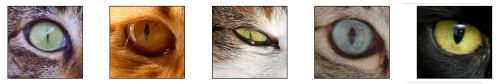
\includegraphics{img/eyes.png}
\caption{}
\end{figure}

\begin{center}\ding{67}\end{center}

Il est généralement préférable d'avoir une idée de départ sur ce que va
faire un programme avant de se mettre à l'écrire\ldots{} Voici le plan :

\begin{enumerate}
\item
  Commencer avec un ensemble de noms de chats ne comprenant que «~Spot
 ~».
\item
  Parcourir chaque e-mail dans l'archive dans l'ordre chronologique.
\item
  Chercher les paragraphes qui commencent par «~Est né le~» ou «~Décédé
  le~».
\item
  Ajouter les noms trouvés dans les paragraphes qui commencent par «~Est
  né le~» à l'ensemble de noms.
\item
  Supprimer les noms de chats trouvés dans les paragraphes qui
  commencent par «~Décédé le~» de notre ensemble.
\end{enumerate}
On extraira les noms d'un paragraphe de la façon suivante :

\begin{enumerate}
\item
  Trouver les deux-points (:) dans le paragraphe.
\item
  Prendre la partie après ce signe.
\item
  Dans cette partie, séparer les noms en cherchant les virgules.
\end{enumerate}
Cet énoncé d'exercice peut rendre nécessaire d'oublier quelques instants
les exceptions possibles et d'accepter aveuglément que tante Émilie
utilise toujours le même format d'écriture, qu'elle n'oublie jamais un
nom de chat, ni ne fait de faute de frappe. Mais votre tante est comme
ça et ça tombe bien pour nous.

\begin{center}\ding{67}\end{center}

D'abord, je vais vous expliquer les propriétés. Beaucoup de valeurs en
JavaScript ont d'autres valeurs qui leur sont associées. Ces
associations sont appelées propriétés. Chaque chaîne de caractères a une
propriété appelée \texttt{length}, (longueur), qui correspond à un
nombre, la quantité de caractères dans cette chaîne.

On peut accéder aux propriétés de deux manières :

\begin{lstlisting}
var texte = "brume pourpre";
show(texte["length"]);
show(texte.length);
\end{lstlisting}
La deuxième manière est un raccourci de la première et ne fonctionne que
lorsque le nom de la propriété s'écrit comme un nom de variable --
lorsqu'il n'y a pas d'espace ou de symbole et lorsqu'elle ne commence
pas par un chiffre.

Les valeurs \texttt{null} et \texttt{undefined} n'ont pas de propriété.
Essayez de lire des propriétés de ces valeurs donnera une erreur.
Essayez le code suivant, juste pour voir le type de message d'erreur que
votre navigateur va retourner dans ce cas de figure (dans certains
navigateurs, ce message sera assez mystérieux).

\begin{lstlisting}
var rienDuTout = null;
show(rienDuTout.length);
\end{lstlisting}
\begin{center}\ding{67}\end{center}

Les propriétés d'une chaîne de caractères ne peuvent pas être changées.
Elles sont plus nombreuses que la seule longueur \texttt{length}, comme
nous allons le voir, mais vous ne pouvez ajouter ni supprimer aucune
propriété.

C'est différent avec les valeurs du type object. Leur rôle principal est
de conserver d'autres valeurs. Ils ont, en quelque sorte, leur propre
jeu de «~tentacules~» sous forme de propriétés. Vous pouvez les
modifier, les supprimer ou en ajouter de nouvelles.

Un objet peut s'écrire de la façon suivante :

\begin{lstlisting}
var chat = {couleur: "gris", nom: "Spot", taille: 46};
chat.taille = 47;
show(chat.taille);
delete chat.taille;
show(chat.taille);
show(chat);
\end{lstlisting}
Comme les variables, chaque propriété attachée à un objet a un nom sous
forme d'une chaîne de caractères. La première instruction crée un objet
dans lequel la propriété \texttt{"couleur"} contient la chaîne
\texttt{"gris"}, la propriété \texttt{"nom"} est liée à la chaîne
\texttt{"Spot"}, et la propriété \texttt{"taille"} fait référence au
nombre \texttt{46}. La deuxième ligne modifie la propriété
\texttt{taille} en lui donnant une nouvelle valeur, ce qui se fait de la
même manière que pour la modification d'une variable.

Le mot-clé \texttt{delete} supprime les propriétés. Essayez de lire une
propriété qui n'existe pas donnera la valeur \texttt{undefined}.

Si une propriété qui n'existe pas encore est affectée avec l'opérateur
\texttt{=}, elle est ajoutée à l'objet.

\begin{lstlisting}
var vide = {};
vide.plusVraiment = 1000;
show(vide.plusVraiment);
\end{lstlisting}
Les propriétés dont le nom ne pourrait pas être une variable doivent
être mises entre guillemets au moment de la création de l'objet et
utilisées avec des parenthèses :

\begin{lstlisting}
var truc = {"gabba gabba": "hey", "5": 10};
show(truc["5"]);
truc["5"] = 20;
show(truc[2 + 3]);
delete truc["gabba gabba"];
\end{lstlisting}
Comme vous pouvez le voir, on peut mettre n'importe quelle expression
entre les parenthèses. Elle sera convertie dans une chaîne pour définir
le nom de la propriété. On peut aussi utiliser des variables pour donner
un nom à une propriété :

\begin{lstlisting}
var nomDePropriete = "length";
var texte = "grandeLigne";
show(texte[nomDePropriete]);
\end{lstlisting}
L'opérateur \texttt{in} peut servir à tester si un objet possède une
certaine propriété. Son résultat est un booléen.

\begin{lstlisting}
var poupeeRusse = {};
poupeeRusse.contenu = poupeeRusse;
show("contenu" in poupeeRusse);
show("contenu" in poupeeRusse.contenu);
\end{lstlisting}
\begin{center}\ding{67}\end{center}

Quand les valeurs d'un objet sont affichées sur la console, on peut
cliquer à la souris pour inspecter leurs propriétés. La fenêtre de
sortie devient une fenêtre «~inspecteur~». Le petit «~x~» en haut à
droite s'utilise pour retourner à la fenêtre de sortie et la flèche
gauche permet de retourner aux propriétés de l'objet inspecté.

\begin{lstlisting}
show(poupeeRusse);
\end{lstlisting}
\begin{center}\ding{67}\end{center}

Ex. 4.1

La solution pour le problème des chats passe par un ensemble de noms. Un
ensemble (ou «~set~») est un groupe de valeurs dans lequel aucune valeur
ne peut apparaître plus d'une fois. Si les noms de chats sont des
chaînes de caractères, pouvez-vous imaginer une façon pour qu'un objet
devienne un ensemble de noms ?

Écrivez maintenant la façon dont un nom peut être ajouté à cet ensemble,
comment on peut le supprimer et comment on peut vérifier si un certain
nom est bien présent dans l'ensemble.

Une solution consiste à mémoriser le contenu de l'ensemble sous la forme
de propriétés d'un objet. Pour ajouter un nom, on crée une propriété
avec ce nom en lui affectant une valeur, n'importe laquelle. Pour
supprimer un nom, on supprimera la propriété de l'objet. L'opérateur
\texttt{in} sera utilisé pour savoir si une certaine propriété fait
partie de l'ensemble\footnote{Il y a quelques problèmes subtils avec cette approche dont nous parlerons et que nous résoudrons dans le \href{chapter8.html}{chapitre 8}. On ne s'en occupera pas pour ce chapitre.}.

\begin{lstlisting}
var set = {"Spot": true};
// Ajoute "Croc Blanc" à l'ensemble
set["Croc Blanc"] = true;
// Supprime "Spot"
delete set["Spot"];
// Regarde si "Asoka" est dans l'ensemble
show("Asoka" in set);
\end{lstlisting}
\begin{center}\ding{67}\end{center}

Les valeurs des objets peuvent apparemment changer. Les types de valeurs
vues dans le \href{chapter2.html}{chapitre 2} sont toutes invariables,
il n'est pas possible de changer une valeur existante pour ces types de
données. Vous pouvez les associer ou en tirer de nouvelles valeurs, mais
lorsque vous prenez une chaîne de caractères particulière, le texte à
l'intérieur ne peut pas être modifié. Avec les objets, d'un autre côté,
le contenu d'une valeur peut être modifié en changeant ses propriétés.

Lorsque nous considérons deux nombres, \texttt{120} et \texttt{120}, il
est possible dans tous les cas pratiques de les considérer comme des
nombres identiques. Avec des objets, il y a une différence importante
entre avoir deux «~références~» du même objet et avoir deux objets
distincts qui possèdent les mêmes propriétés. Considérons le code
suivant :

\begin{lstlisting}
var objet1 = {valeur: 10};
var objet2 = objet1;
var objet3 = {valeur: 10};

show(objet1 == objet2);
show(objet1 == objet3);

objet1.valeur = 15;
show(objet2.valeur);
show(objet3.valeur);
\end{lstlisting}
\texttt{objet1} et \texttt{objet2} sont deux variables attachées à la
\emph{même} valeur. Il n'y a en fait qu'un seul objet, c'est pourquoi en
changeant \texttt{objet1} on change également la valeur de
\texttt{objet2}. La variable \texttt{objet3} pointe vers un autre objet
qui contient au départ la même propriété que \texttt{objet1} mais elle a
une existence distincte.

L'opérateur JavaScript \texttt{==}, lorsqu'il compare des objets, ne
retournera la valeur booléenne \texttt{true} que si chacune des valeurs
qu'on lui donne à comparer sont exactement les mêmes. Comparer des
objets différents ayant des contenus identiques donnera le résultat
\texttt{false}. C'est utile dans certaines situations, mais peu adapté à
d'autres.

\begin{center}\ding{67}\end{center}

Les valeurs d'un objet peuvent jouer de nombreux rôles. Se comporter
comme un ensemble n'est que l'un d'entre eux. Nous allons voir d'autres
utilisations dans ce chapitre et le \href{chapter8.html}{chapitre 8}
montrera d'autres façons importantes d'utiliser les objets.

Dans le plan d'action pour le problème des chats --- en fait,
appelons-le un \emph{algorithme} au lieu d'un plan, cela nous donne
l'impression qu'on sait de quoi on parle --- dans l'algorithme, on parle
de parcourir chaque e-mail contenu dans une archive. Mais comment se
présente cette archive ? Et d'où vient-elle ?

Ne vous inquiétez pas de la deuxième question pour le moment. Le
\href{chapter14.html}{chapitre 14} explique quelques-unes des
possibilités pour importer des données dans vos programmes. Pour
l'instant, on dira que les e-mails sont déjà là, comme par magie. La
magie est parfois très facile, avec les ordinateurs.

\begin{center}\ding{67}\end{center}

La façon dont l'archive est enregistrée reste une question pertinente.
Elle contient quantité d'e-mails. Un e-mail peut être vu comme une
chaîne de caractères, c'est évident. Toute l'archive pourrait être mise
dans une énorme chaîne de caractères mais ce ne serait pas pratique. Ce
qu'il nous faut, c'est une structure de chaînes de caractères
distinctes.

Les objets sont justement utilisés pour structurer des choses. On
pourrait très bien créer un objet comme celui-ci :

\begin{lstlisting}
var archiveDeMails = {"le premier e-mail": "Mon cher neveu, ...",
                   "le deuxième e-mail": "..."
                   /* et ainsi de suite... */};
\end{lstlisting}
Mais parcourir les e-mails du début à la fin serait difficile ---
comment le programme peut-il deviner le nom de ces propriétés ? La
solution est d'utiliser des noms de propriétés plus prévisibles :

\begin{lstlisting}
var archiveDeMails = {0: "Mon cher neveu, ... (mail numéro 1)",
                   1: "(mail numéro 2)",
                   2: "(mail numéro 3)"};

for (var courant = 0; courant in archiveDeMails; courant++)
  print("Traitement de l'e-mail #", courant, ": ", archiveDeMails[courant]);
\end{lstlisting}
La chance veut qu'il existe un type d'objet particulier qui corresponde
exactement à ce type de besoin. Ce sont les tableaux et ils fournissent
des commodités très utiles, comme par exemple \texttt{length}
(longueur), une propriété qui contient le nombre d'éléments dans le
tableau et bien d'autres fonctions utiles pour ce type de structure.

Pour créer de nouveaux tableaux on utilise des crochets (\texttt{{[}} et
\texttt{{]}}):

\begin{lstlisting}
var archiveDeMails = ["mail un", "mail deux", "mail trois"];

for (var courant = 0; courant < archiveDeMails.length; courant++)
  print("Traitement de l'e-mail #", courant, ": ", archiveDeMails[courant]);
\end{lstlisting}
Dans cet exemple, le nombre d'éléments n'est plus spécifié
explicitement. Le premier a automatiquement le numéro 0, le deuxième le
numéro 1 et ainsi de suite.

Pourquoi commencer à 0 ? Dans la vie courante on compte d'habitude à
partir de 1. Aussi étrange que cela paraisse, la numérotation à partir
de 0 est souvent plus pratique pour programmer. Faites avec pour
l'instant, vous allez vous y faire.

Commencer par l'élément 0 veut aussi dire que dans une structure qui a
\texttt{X} éléments, le dernier élément sera trouvé à la position
\texttt{X - 1}. C'est pourquoi la boucle \texttt{for} dans notre exemple
teste la valeur \texttt{current \textless{} archiveDeMails.length}. Il
n'y a pas d'élément à la position \texttt{archiveDeMails.length}, donc
dès que \texttt{current} atteint cette valeur, on arrête la boucle.

\begin{center}\ding{67}\end{center}

Ex. 4.2

Écrivez une fonction nommée \texttt{serie} qui prend un argument, un
nombre positif et retourne un tableau contenant chaque nombre de 0
jusqu'au nombre donné en paramètre inclus.

Un tableau vide peut être créé en tapant simplement \texttt{{[}{]}}.
Souvenez-vous que pour ajouter des propriétés à un tableau, comme pour
un objet, il suffit d'affecter une valeur à la propriété avec
l'opérateur \texttt{=}. La propriété \texttt{length} est mise à jour
automatiquement quand des éléments sont ajoutés.

\begin{lstlisting}
function serie(max) {
  var resultat = [];
  for (var i = 0; i <= max; i++)
    resultat[i] = i;
  return resultat;
}
show(serie(4));
\end{lstlisting}
Au lieu de nommer la variable de boucle \texttt{compteur} ou
\texttt{courant}, comme je l'ai fait jusqu'à présent, elle s'appelle
désormais simplement \texttt{i}. L'utilisation d'une seule lettre,
habituellement \texttt{i}, \texttt{j} ou \texttt{k} pour les variables
de boucle est une habitude très répandue en programmation. Son origine
tient presque à de la paresse : on préfère taper un caractère que sept
et des noms comme \texttt{compteur} et \texttt{courant} ne donnent pas
forcément plus d'informations sur la variable.

Si un programme utilise trop souvent des variables à un seul caractère,
sans explication, il peut devenir très difficile à comprendre. Dans mes
propres programmes, j'essaie de me limiter à quelques cas de figures
seulement. Les petites boucles font partie de ces cas. Si la boucle
contient une autre boucle et que celle-ci utilise aussi une variable
appelée \texttt{i}, la boucle intérieure va modifier la variable dont se
sert la première boucle, et rien ne va fonctionner. Ou pourrait utiliser
\texttt{j} pour la boucle intérieure, mais en général, lorsque le corps
d'une boucle est grand, vous devriez utiliser un nom de variable ayant
une signification utile pour la compréhension.

\begin{center}\ding{67}\end{center}

Les objets chaînes de caractères et tableaux contiennent tous deux,
outre la propriété \texttt{length}, un certain nombre d'autres
propriétés qui font référence à des fonctions.

\begin{lstlisting}
var doh = "Doh";
print(typeof doh.toUpperCase);
print(doh.toUpperCase());
\end{lstlisting}
Chaque chaîne de caractères a une propriété \texttt{toUpperCase}.
Lorsqu'elle est appelée, elle retourne une copie de la chaîne,
transformée avec chaque lettre en majuscule. Il y a aussi l'équivalent
\texttt{toLowerCase}. Devinez le résultat\ldots{}

Remarquez que même si l'appel de \texttt{toUpperCase} se fait sans
arguments, la fonction a malgré tout accès au contenu de la chaîne de
caractères \texttt{"Doh"}, la valeur dont elle est une propriété. La
façon dont cela fonctionne est décrite dans le
\href{chapter8.html}{chapitre 8}.

Les propriétés qui se comportent comme des fonctions sont généralement
appelées méthodes, ainsi, \texttt{toUpperCase} est une méthode des
objets chaînes de caractères.

\begin{lstlisting}
var flipper = [];
flipper.push("Flipper");
flipper.push("le");
flipper.push("dauphin");
show(flipper.join(" "));
show(flipper.pop());
show(flipper);
\end{lstlisting}
La méthode \texttt{push}, associée aux tableaux, peut être utilisée pour
ajouter des valeurs à ceux-ci. Nous aurions pu l'utiliser dans
l'exercice précédent, à la place de \texttt{resultat{[}i{]} = i}. Il y a
aussi la méthode \texttt{pop}, complémentaire de \texttt{push} : elle
supprime le dernier élément d'un tableau et retourne sa valeur.
\texttt{join} construit une seule chaîne de caractères à partir d'un
tableau de chaînes de caractères. Le paramètre utilisé avec cette
méthode sera inséré entre chaque valeur du tableau, avant l'assemblage
de la chaîne de caractères finale.

\begin{center}\ding{67}\end{center}

Revenons à nos chats : nous savons maintenant qu'utiliser un tableau
serait une bonne idée pour ranger les archives des e-mails. Sur cette
page, la fonction \texttt{recupererLesMails} sera utilisée pour
récupérer (magiquement) ce tableau. Parcourir les emails qu'il contient
pour les traiter un par un devient simple comme un jeu d'enfant :

\begin{lstlisting}
var archiveDeMails = recupererLesMails();

for (var i = 0; i < archiveDeMails.length; i++) {
  var email = archiveDeMails[i];
  print("Traitement de l'e-mail #", i);
  // Faire plus de choses...
}
\end{lstlisting}
Nous avons également décidé d'une manière de représenter un ensemble de
chats vivants. Le problème qui reste à traiter, cependant, est celui de
détecter des paragraphes d'un e-mail qui contiennent
\texttt{"Est né le"} ou \texttt{"Décédé le"}.

\begin{center}\ding{67}\end{center}

La première question qui vient à l'esprit est de savoir ce qu'est un
paragraphe au juste. Dans ce cas, la valeur de la chaîne elle-même n'est
pas d'une grande utilité : le concept du texte en JavaScript ne va guère
plus loin que l'idée de «~suite de caractères~», si bien que nous devons
définir les paragraphes de cette façon.

Nous avons vu plus haut qu'il existe une chose qui s'appelle un
caractère de fin de ligne. C'est ce que la plupart des gens utilisent
pour séparer les paragraphes. Nous considérons donc un paragraphe comme
une partie de mail qui commence par un caractère saut de ligne ou au
début du contenu du message et se termine au caractère saut de ligne
suivant ou bien à la fin du contenu.

Et nous n'avons même pas à écrire nous-mêmes l'algorithme pour scinder
une chaîne en paragraphes. Les chaînes ont déjà une méthode appelée
\texttt{split}, qui est (pratiquement) l'inverse de la méthode
\texttt{join} pour les tableaux. Elle découpe une chaîne en un tableau
en utilisant la chaîne fournie comme argument pour déterminer à quel
endroit opérer les divisions en paragraphes.

\begin{lstlisting}
var mots = "Les villes de l'arrière-pays";
show(mots.split(" "));
\end{lstlisting}
Ainsi, découper avec des caractères saut de ligne
(\texttt{"\textbackslash{}n"}) est une méthode utilisable pour diviser
un e-mail en paragraphes.

\begin{center}\ding{67}\end{center}

Ex. 4.3

\texttt{split} et \texttt{join} ne sont pas exactement l'inverse l'une
de l'autre. \texttt{string.split(x).join(x)} produit toujours la valeur
originale, mais pas \texttt{array.join(x).split(x)}. Pouvez-vous donner
un exemple de tableau dans lequel \texttt{.join(" ").split(" ")} produit
une valeur différente ?

\begin{lstlisting}
var tableau = ["a", "b", "c d"];
show(tableau.join(" ").split(" "));
\end{lstlisting}
\begin{center}\ding{67}\end{center}

Les paragraphes qui ne commencent ni par «~Né le~» ni par «~Décédé le~»
peuvent être ignorés par le programme. Comment peut-on tester si une
chaîne commence par un mot particulier ? On peut utiliser la méthode
\texttt{charAt} pour obtenir un caractère particulier dans une chaîne.
\texttt{x.charAt(0)} donne le premier caractère, \texttt{1} est le
deuxième et ainsi de suite. Voici une façon de vérifier si une chaîne
commence par «~Né le» :

\begin{lstlisting}
var paragraphe = "Est né le 15/11/2003 (mère, Spot) : Croc Blanc";
show(paragraphe.charAt(0) == "E" && paragraphe.charAt(1) == "s" &&
     paragraphe.charAt(2) == "t" && paragraphe.charAt(3) == " " &&
     paragraphe.charAt(4) == "n" && paragraphe.charAt(5) == "é" &&
     paragraphe.charAt(6) == " " && paragraphe.charAt(7) == "l" &&
     paragraphe.charAt(8) == "e");
\end{lstlisting}
Mais cela devient un peu pénible -- imaginez que vous devez vérifier la
présence d'un mot de 30 caractères. On peut cependant en tirer une leçon
utile : si une ligne est démesurément longue, on peut l'étendre sur
plusieurs lignes. Le résultat peut être plus facile à lire en alignant
le début d'une nouvelle ligne avec la ligne originale jouant le même
rôle

Les chaînes possèdent également une méthode nommée \texttt{slice}. Elle
permet de copier un morceau de la chaîne de caractères, en commençant
par le caractère à la position donnée par le premier argument, et se
terminant avant le caractère (non inclus) à la position donnée par le
second argument. Cela permet de vérifier une chaîne de caractères en peu
de lignes.

\begin{lstlisting}
show(paragraphe.slice(0, 9) == "Est né le");
\end{lstlisting}
\begin{center}\ding{67}\end{center}

Ex. 4.4

Écrivez une fonction nommée \texttt{chaineCommencePar} qui prend deux
arguments, tous les deux des chaînes de caractères. Elle renvoie
\texttt{true} quand le premier argument commence avec les caractères du
second arguments, sinon elle renvoie \texttt{false}.

\begin{lstlisting}
function chaineCommencePar(chaine, motif) {
  return chaine.slice(0, motif.length) == motif;
}

show(chaineCommencePar("rotation", "rot"));
\end{lstlisting}
\begin{center}\ding{67}\end{center}

Que se passe-t-il quand \texttt{charAt} ou \texttt{slice} sont utilisés
pour prendre un fragment de chaîne qui n'existe pas ? Est-ce que la
fonction \texttt{chaineCommencePar} que j'ai montrée va encore
fonctionner si la chaîne recherchée est plus longue que celle dans
laquelle on cherche ?

\begin{lstlisting}
show("Ouai".charAt(250));
show("Nan".slice(1, 10));
\end{lstlisting}
\texttt{charAt} va renvoyer \texttt{""} s'il n'existe pas de caractère à
la position donnée et \texttt{slice} va tout simplement laisser tomber
la partie de la nouvelle chaîne qui n'existe pas.

Cela confirme que cette version de \texttt{chaineCommencePar}
fonctionne. Quand la fonction
\texttt{chaineCommencePar("Idiots","Mes très chers collègues")} est
appelée, l'appel à \texttt{slice} renverra toujours une chaîne plus
courte que \texttt{motif}, parce que le premier argument,
\texttt{chaine} ne comporte pas assez de caractères. C'est pour cette
raison que la comparaison avec \texttt{==} renverra \texttt{false}, ce
qui est correct.

C'est une bonne idée de toujours consacrer un moment pour prendre en
considération les entrées aberrantes (mais valides) dans un programme.
On les appelle en général des cas imprévus et il est très fréquent qu'un
programme qui tourne à merveille avec toutes les entrées «~normales~» se
plante complètement avec des cas imprévus.

\begin{center}\ding{67}\end{center}

La seule partie de notre problème de chats qui ne soit pas encore
résolue est l'extraction des noms d'un paragraphe. L'algorithme était le
suivant :

\begin{enumerate}
\item
  Trouver le deux-points (:) dans le paragraphe.
\item
  Prendre la partie après ce signe.
\item
  Dans cette partie, séparer les noms en cherchant les virgules.
\end{enumerate}
Il faut reproduire cela à la fois pour les paragraphes qui commencent
par \texttt{Décés le} et ceux qui commencent par \texttt{Est né le}. Ce
serait une bonne idée de le mettre dans une fonction, de sorte que les
deux parties de code qui gèrent les différentes sortes de paragraphes
puissent l'utiliser.

\begin{center}\ding{67}\end{center}

Ex. 4.5

Savez-vous écrire une fonction \texttt{nomDesChats} qui prenne un
paragraphe comme argument et renvoie un tableau de noms ?

Les chaînes ont une méthode \texttt{indexOf}que l'on peut utiliser pour
trouver la (première) position d'un caractère ou une sous-chaîne à
l'intérieur d'une chaîne. De même si on ne donne qu'un seul argument à
\texttt{slice}, elle renverra la partie de la chaîne depuis la première
position jusqu'à son extrémité.

Il peut être pratique d'utiliser la console pour «~explorer~» les
fonctions. Par exemple, tapez \texttt{"foo: bar".indexOf(":")} et voyez
ce qui se passe. (NdT: les mots \texttt{foo} et \texttt{bar} n'ont pas
de signification précise, et illustrent parfois des exemples de code).

\begin{lstlisting}
function nomDesChats(paragraphe) {
  var deuxPoints = paragraphe.indexOf(":");
  return paragraphe.slice(deuxPoints + 2).split(", ");
}

show(nomDesChats("Est né le 20/09/2004 (mère, Bess la Jaune): " +
              "Docteur Hobbles II, Kaira"));
\end{lstlisting}
La partie la plus délicate qui est ignorée par la description originale
de l'algorithme, est le traitement des espaces après les deux-points et
les virgules. Le \texttt{+2}, utilisé pour le découpage de chaînes, est
nécessaire pour laisser de côté le deux-points lui-même et l'espace qui
le suit. L'argument pour \texttt{split} contient à la fois une virgule
et un espace, parce que ce sont les séparateurs de noms, plutôt que par
une simple virgule.

Cette fonction n'effectue aucune vérification de problèmes éventuels.
Nous faisons comme si, dans ce cas précis, l'entrée était toujours
correcte.

\begin{center}\ding{67}\end{center}

Tout ce qui nous reste à faire maintenant, c'est de rassembler les
pièces du puzzle. Voici une façon de s'y prendre :

\begin{lstlisting}
var archiveDeMails = recupererLesMails();
var chatsVivants = {"Spot": true};

for (var mail = 0; mail < archiveDeMails.length; mail++) {
  var paragraphes = archiveDeMails[mail].split("\n");
  for (var paragraphe = 0;
       paragraphe < paragraphes.length;
       paragraphe++) {
    if (chaineCommencePar(paragraphes[paragraphe], "Est né le")) {
      var noms = nomDesChats(paragraphes[paragraphe]);
      for (var nom = 0; nom < noms.length; nom++)
        chatsVivants[noms[nom]] = true;
    }
    else if (chaineCommencePar(paragraphes[paragraphe], "Décédé le")) {
      var noms = nomDesChats(paragraphes[paragraphe]);
      for (var nom = 0; nom < noms.length; noms++)
        delete chatsVivants[noms[nom]];
    }
  }
}

show(chatsVivants);
\end{lstlisting}
Voilà un bloc de code assez copieux et dense. Nous allons voir tout de
suite comment l'alléger un peu. Mais d'abord jetons un coup d'œil aux
résultats. Nous savons comment vérifier si un chat particulier a survécu
:

\begin{lstlisting}
if ("Spot" in chatsVivants)
  print("Spot est vivant !");
else
  print("Ce bon vieux Spot, qu'il repose en paix.");
\end{lstlisting}
Mais comment allons-nous faire pour dresser la liste de tous les chats
vivants ? Le mot-clé \texttt{in} a une signification légèrement
différente lorsqu'il est utilisé avec \texttt{for} :

\begin{lstlisting}
for (var chat in chatsVivants)
  print(chat);
\end{lstlisting}
Une boucle comme celle-là va parcourir les noms des propriétés d'un
objet, ce qui nous permettra d'énumérer tous les noms de notre ensemble.

\begin{center}\ding{67}\end{center}

Certaines parties de code ressemble à une jungle impénétrable. L'exemple
de solution pour le problème des chats souffre de ce défaut. Une façon
de ménager des clairières consiste tout simplement à ajouter des lignes
vides. Cela améliore la lisibilité, mais ne résout pas véritablement le
problème.

Ce qu'il nous faut ici, c'est casser le code. Nous avons déjà écrit deux
fonctions d'aide, \texttt{chaineCommencePar} et \texttt{nomDesChats},
qui toutes deux résolvent une petite partie du problème de façon
compréhensible. Continuons sur cette lancée.

\begin{lstlisting}
function ajouterAuSet(set, valeurs) {
  for (var i = 0; i < valeurs.length; i++)
    set[valeurs[i]] = true;
}

function enleverDuSet(set, valeurs) {
  for (var i = 0; i < valeurs.length; i++)
    delete set[valeurs[i]];
}
\end{lstlisting}
Ces deux fonctions traitent de l'ajout et de la suppression des noms
dans l'ensemble. Ce qui supprime déjà les deux plus importantes boucles
internes de la solution :

\begin{lstlisting}
var chatsVivants = {Spot: true};

for (var mail = 0; mail < archiveDeMails.length; mail++) {
  var paragraphes = archiveDeMails[mail].split("\n");
  for (var paragraphe = 0;
       paragraphe < paragraphes.length;
       paragraphe++) {
    if (chaineCommencePar(paragraphes[paragraphe], "Est né le"))
      ajouterAuSet(chatsVivants, nomDesChats(paragraphes[paragraphe]));
    else if (chaineCommencePar(paragraphes[paragraphe], "Décédé le"))
      enleverDuSet(chatsVivants, nomDesChats(paragraphes[paragraphe]));
  }
}
\end{lstlisting}
C'est un sacré progrès, si je peux me permettre. Pourquoi
\texttt{ajouterAuSet} et \texttt{enleverDuSet} prennent-ils l'ensemble
comme argument ? Ils pourraient utiliser la variable
\texttt{chatsVivants} directement, s'ils le voulaient. La raison, c'est
que de cette façon elles ne sont pas totalement liées à notre problème.
Si \texttt{ajouterAuSet} changeait directement \texttt{chatsVivants}, il
faudrait l'appeler \texttt{ajouterChatsDansEnsembleDeChats} ou quelque
chose comme ça. Tel que nous l'utilisons, c'est un outil utile pour des
cas plus généraux.

Même si nous ne devions jamais utiliser ces fonctions pour quoi que ce
soit d'autre, ce qui est très probable, il est utile de les décrire de
cette façon. Car elles se «~suffisent à elles-même~», on peut les lire
et les comprendre, sans avoir besoin de connaître une variable externe
nommée \texttt{chatsVivants}.

Ces fonctions ne sont pas pures : elles modifient l'objet \texttt{set}
qui a été passé en premier argument. Cela rend les choses un peu plus
délicates qu'avec des fonctions pures mais c'est déjà beaucoup moins
perturbant que des fonctions qui perdent les pédales et modifient les
valeurs de variables comme ça leur chante.

\begin{center}\ding{67}\end{center}

Nous continuons à découper l'algorithme en petites unités :

\begin{lstlisting}
function trouverChatsVivants() {
  var archiveDeMails = recupererLesMails();
  var chatsVivants = {"Spot": true};

  function traiterParagraphe(paragraphe) {
    if (chaineCommencePar(paragraphe, "Est né le"))
      ajouterAuSet(chatsVivants, nomDesChats(paragraphe));
    else if (chaineCommencePar(paragraphe, "Décédé le"))
      enleverDuSet(chatsVivants, nomDesChats(paragraphe));
  }

  for (var mail = 0; mail < archiveDeMails.length; mail++) {
    var paragraphes = archiveDeMails[mail].split("\n");
    for (var i = 0; i < paragraphes.length; i++)
      traiterParagraphe(paragraphes[i]);
  }
  return chatsVivants;
}

var combien = 0;
for (var chat in trouverChatsVivants())
  combien++;
print("Il y a ", combien, " chats.");
\end{lstlisting}
La totalité de l'algoritme est encapsulée dans une fonction. Cela
signifie qu'elle ne laisse rien traîner en vrac derrière elle après
exécution : \texttt{chatsVivants} est maintenant une variable locale
dans la fonction et non plus une variable globale, si bien qu'elle
n'existe que pendant que la fonction s'exécute. Le code qui a besoin de
cet ensemble peut appeler \texttt{trouverChatsVivants} et utiliser la
valeur qu'il renvoie.

Il me semble que faire de \texttt{traiterParagraphe} une fonction
distincte peut aussi clarifier les choses. Mais celle-ci est si
étroitement liée à l'algorithme-des-chats qu'elle n'aurait aucun sens
dans une autre situation. De plus, elle a besoin d'accéder à la variable
\texttt{chatsVivants}. C'est donc une candidate parfaite pour devenir
une fonction à l'intérieur d'une fonction. Quand elle existe à
l'intérieur de \texttt{trouverChatsVivants}, il est clair qu'elle n'est
pertinente que là et qu'elle a accès aux variables de sa fonction
parente.

Cette solution est en fait plus \emph{grande} que la précédente. Mais
elle est plus propre et j'espère que vous reconnaîtrez qu'elle est plus
lisible.

\begin{center}\ding{67}\end{center}

Le programme ignore encore un grand nombre d'informations qui sont
incluses dans les mails. Il s'agit des dates de naissance, de mort et
des noms des mères.

Commençons avec les dates : quelle pourrait être la meilleure façon de
stocker une date ? Nous pourrions créer un objet avec ces trois
propriétés, \texttt{year}, \texttt{month}, et \texttt{day} et stocker
ensuite des nombres à l'intérieur.

\begin{lstlisting}
var quand = {year: 1980, month: 2, day: 1};
\end{lstlisting}
Mais JavaScript fournit déjà une sorte d'objet pour cela. Un tel objet
peut être créé en utilisant le mot-clé \texttt{new}:

\begin{lstlisting}
var quand = new Date(1980, 1, 1);
show(quand);
\end{lstlisting}
Tout comme la notation avec les accolades et les deux-points que nous
avons déjà vue, \texttt{new} est une façon de créer des valeurs d'un
objet. Au lieu de préciser tous les noms de propriétés et les valeurs,
une fonction est utilisée pour créer l'objet. Cela rend possible de
définir une sorte de procédure standard pour créer des objets. Les
fonctions comme celle-là s'appellent constructeurs et nous verrons
comment les écrire dans \href{chapter8.html}{chapitre 8}.

Le constructeur \texttt{Date} peut être utilisé de différentes manières

\begin{lstlisting}
show(new Date());
show(new Date(1980, 1, 1));
show(new Date(2007, 2, 30, 8, 20, 30));
\end{lstlisting}
Comme vous pouvez le voir, ces objets peuvent enregistrer l'heure d'un
jour aussi bien qu'une date. Quand aucun argument n'est précisé, un
objet réprésentant l'heure et la date actuelles est créé. Des arguments
peuvent être précisés pour stocker une heure et une date précises.
L'ordre des arguments est l'année, le mois, le jour, l'heure, la minute,
la seconde puis la milliseconde. Les quatre derniers arguments sont
optionnels et définis à 0 s'il ne sont pas précisés.

Pour décrire les mois, on utilise la numérotation de 0 à 11, qui peut
provoquer une confusion. Surtout que les nombres définissant les jours
commencent eux à 1.

\begin{center}\ding{67}\end{center}

Le contenu de l'objet \texttt{Date} peut être inspecté avec un nombre de
méthodes \texttt{get\ldots{}}.

\begin{lstlisting}
var aujourdhui = new Date();
print("Année : ", aujourdhui.getFullYear(), ", mois : ",
      aujourdhui.getMonth(), ", jour : ", aujourdhui.getDate());
print("Heure : ", aujourdhui.getHours(), ", minutes : ",
      aujourdhui.getMinutes(), ", secondes: ", aujourdhui.getSeconds());
print("Jour de la semaine : ", aujourdhui.getDay());
\end{lstlisting}
Tous ces éléments, expecté la méthode \texttt{getDay}, ont une variable
\texttt{set...} qui peut être utilisée pour modifier la valeur de
l'objet date.

Dans l'objet, une date est représentée par la somme de millisecondes
cumulée depuis le 1er Janvier 1970. Vous pouvez imaginer que c'est un
nombre assez impressionnant.

\begin{lstlisting}
var aujourdhui = new Date();
show(aujourdhui.getTime());
\end{lstlisting}
Une chose très utile à faire avec les dates, c'est de les comparer.

\begin{lstlisting}
var chuteDuMur = new Date(1989, 10, 9);
var premiereGuerreDuGolf = new Date (1990, 6, 2);
show(chuteDuMur < premiereGuerreDuGolf);
show(chuteDuMur == chuteDuMur);
// mais
show(chuteDuMur == new Date(1989, 10, 9));
\end{lstlisting}
Comparer les dates avec \texttt{\textless{}}, \texttt{\textgreater{}},
\texttt{\textless{}=} et \texttt{\textgreater{}=} remplit exactement
l'office que nous voulons en faire. Quand un objet date est comparé avec
lui-même, le résultat est \texttt{true}, ce qui est bien également. Mais
quand \texttt{==} est utilisé pour comparer un objet date à un autre
objet date différent mais de même valeur, on obtient \texttt{false}.
Etrange, non ?

Comme précisé plus tôt, \texttt{==} retournera la valeur
\href{lors\%20de\%20la\%0Acomparaison\%20de\%20deux\%20éléments\%20différents,\%20même\%20si\%20ces\%20deux\%20éléments\%0Acontiennent\%20les\%20mêmes\%20propriétés.\%20Ceci\%20est\%20un\%20peu\%20maladroit\%20et\%20sujet\%0Aà\%20erreur,\%20puisqu''on\%20s'attendrait\%20à\%20ce\%20que\%20\textbar{}\textgreater{}=\textbar{}\%20et\%20\textbar{}==\textbar{}\%20aient\%20le\%20même\%0Acomportement.\%20Pour\%20tester\%20si\%20deux\%20dates\%20sont\%20égales,\%20peut\%20être\%20fait\%20de\%0Acette\%20manière\%A0:}{false}

\begin{lstlisting}
var chuteDuMur1 = new Date(1989, 10, 9),
chuteDuMur2 = new Date(1989, 10 ,9);
show(chuteDuMur1.getTime() == chuteDuMur2.getTime());
\end{lstlisting}
\begin{center}\ding{67}\end{center}

\begin{center}\ding{67}\end{center}

Au-delà de la date et l'heure, l'objet \texttt{Date} contient aussi des
informations sur le fuseau horaire. Quand il est une heure à Amsterdam,
en fonction de la période de l'année il peut être midi à Londres et sept
heures du matin à New York. De telles heures ne peuvent être rapprochées
que si vous prenez les fuseaux horaires en compte. La fonction
\texttt{getTimezoneOffset} d'une \texttt{Date} peut être utilisée pour
trouver de combien de minutes elle s'éloigne du GMT (Heure du méridien
de Greenwich)

\begin{lstlisting}
var maintenant = new Date();
print(maintenant.getTimezoneOffset());
\end{lstlisting}
\begin{center}\ding{67}\end{center}

Ex. 4.6

\begin{lstlisting}
"Décédé le 27/04/2006 : Black Leclère"
\end{lstlisting}
La partie date est toujours exactement à la même place du paragraphe.
Comme c'est pratique. Écrivez une fonction \texttt{extraireDate} qui
prend un tel paragraphe pour argument, extrait la date et la renvoit
sous la forme d'un objet date.

\begin{lstlisting}
function extraireDate(paragraphe) {
  function nombreEnPosition(position, longueur) {
    return Number(paragraphe.slice(position, position + longueur));
  }
  return new Date(nombreEnPosition(16, 4), nombreEnPosition(13, 2) - 1,
                  nombreEnPosition(10, 2));
}

show(extraireDate("Décédé le 27-04-2006 : Black Leclère"));
\end{lstlisting}
Cela marcherait sans les appels à \texttt{Number}, mais comme je l'ai
expliqué plus haut, je préfère ne pas utiliser de chaînes comme si elles
étaient des nombres. La fonction interne a été introduite pour éviter
d'avoir à répéter trois fois les parties \texttt{Number} et
\texttt{slice}.

Notez le \texttt{-1} pour le numéro du mois. Comme la plupart des gens,
tante Émilie compte les mois à partir de 1, nous devons donc ajuster
cette valeur avant de donner la \texttt{Date} au constructeur (le numéro
du jour ne relève pas du même problème, puisque les objets \texttt{Date}
compte les jours de la façon humaine habituelle).

Dans le \href{chapter10.html}{chapitre 10}, nous verrons une façon plus
pratique et plus sûre d'extraire des parties de chaînes qui ont une
structure déterminée.

\begin{center}\ding{67}\end{center}

Stocker des chats est une opération qui va se dérouler différemment à
partir de maintenant. Au lieu de simplement mettre la valeur
\texttt{true} sur l'ensemble, nous stockons un objet avec les
informations sur le chat. Lorsqu'un chat meurt, nous ne le supprimons
pas de l'ensemble, nous ajoutons simplement la propriété \texttt{deces}
à l'objet pour stocker la date à laquelle le pauvre animal a trépassé.

Cela signifie que nos fonctions \texttt{ajouterAuSet} et
\texttt{enleverDuSet} sont devenues inutiles. Quelque chose de
comparable est nécessaire, mais il s'agit de stocker aussi les dates de
naissance et par la suite, les noms des mères.

\begin{lstlisting}
function enregistrementChat(nom, dateNaissance, mere) {
  return {nom: nom, naissance: dateNaissance, mere: mere};
}

function ajouterChats(set, noms, dateNaissance, mere) {
  for (var i = 0; i < noms.length; i++)
    set[noms[i]] = enregistrementChat(noms[i], dateNaissance, mere);
}
function chatsDecedes(set, noms, dateDeces) {
  for (var i = 0; i < noms.length; i++)
    set[noms[i]].deces = dateDeces;
}
\end{lstlisting}
\texttt{enregistrementChat} est une fonction distincte pour créer ces
objets de stockage. Elle pourrait être utile dans d'autres situations,
telles que la création d'un objet pour Spot. «~Record~» («
enregistrement~» en français) est le terme qu'on emploie couramment pour
des objets de ce type, qui sont utilisés pour regrouper un nombre limité
de valeurs.

\begin{center}\ding{67}\end{center}

Essayons donc maintenant d'extraire les noms des mamans chats qui se
trouvent dans des paragraphes.

\begin{lstlisting}
"Est né le 15/11/2003 (mère, Spot): Croc Blanc"
\end{lstlisting}
Voici un moyen d'obtenir cela\ldots{}

\begin{lstlisting}
function extraireNomMere(paragraphe) {
  var start = paragraphe.indexOf("(mère, ") + "(mère, ".length;
  var end = paragraphe.indexOf(")");
  return paragraphe.slice(start, end);
}

show(extraireNomMere("Est né le 15/11/2003 (mère, Spot): Croc Blanc"));
\end{lstlisting}
Notez comment la position de départ a dû être ajustée à la longueur de
\texttt{"(mère, "}, parce que \texttt{indexOf} renvoie la position
initiale de la chaîne et non la finale.

\begin{center}\ding{67}\end{center}

Ex. 4.7

Ce que fait \texttt{extraireNomMere} peut être exprimé d'une façon plus
générale. Écrivez une fonction \texttt{extraireChaineEntre} qui prend
trois arguments, qui seront tous des chaînes. Elle renverra la partie du
premier argument qui apparaît entre les chaînes fournies par le deuxième
et le troisième argument.

Ainsi,
\texttt{extraireChaineEntre("Est né le 15/11/2003 (mère, Spot): Croc Blanc", "(mère, ", ")")}
donne \texttt{"Spot"}.

\texttt{extraireChaineEntre("bu {]} boo {[} bah {]} gzz", "{[} ", " {]}")}
renvoie \texttt{"bah"}.

Pour faire marcher ce deuxième exemple, il peut être utile de savoir
qu'on peut attribuer à \texttt{indexOf} un second paramètre facultatif
qui précise à partir de quel point doit commencer la recherche.

\begin{lstlisting}
function extraireChaineEntre(chaine, debut, fin) {
  var indexDebut = chaine.indexOf(debut) + debut.length;
  var indexFin = chaine.indexOf(fin, indexDebut);
  return chaine.slice(indexDebut, indexFin);
}
show(extraireChaineEntre("bu ] boo [ bah ] gzz", "[ ", " ]"));
\end{lstlisting}
\begin{center}\ding{67}\end{center}

Avoir la fonction \texttt{extraireChaineEntre} rend possible
l'expression de extraireNomMere de façon plus simple :

\begin{lstlisting}
function extraireNomMere(paragraphe) {
  return extraireChaineEntre(paragraphe, "(mère, ", ")");
}
\end{lstlisting}
\begin{center}\ding{67}\end{center}

Le nouvel algorithme à chats amélioré ressemble maintenant à ça :

\begin{lstlisting}
function trouverChats() {
  var archiveDeMails = recupererLesMails();
  var chats = {"Spot": enregistrementChat("Spot", new Date(1997, 2, 5),
              "inconnue")};

  function traiterParagraphe(paragraphe) {
    if (chaineCommencePar(paragraphe, "Est né le"))
      ajouterChats(chats, nomDesChats(paragraphe), extraireDate(paragraphe),
              extraireNomMere(paragraphe));
    else if (chaineCommencePar(paragraphe, "Décédé le"))
      chatsDecedes(chats, nomDesChats(paragraphe), extraireDate(paragraphe));
  }

  for (var mail = 0; mail < archiveDeMails.length; mail++) {
    var paragraphes = archiveDeMails[mail].split("\n");
    for (var i = 0; i < paragraphes.length; i++)
      traiterParagraphe(paragraphes[i]);
  }
  return chats;
}

var tousLesChats = trouverChats();
\end{lstlisting}
Avoir ces données supplémentaires nous permet d'avoir finalement une
idée plus précise des chats dont parle tante Émilie. Une fonction comme
celle-ci pourrait être utile :

\begin{lstlisting}
function formatDate(date) {
  return date.getDate() + "/" + (date.getMonth() + 1) +
         "/" + date.getFullYear();
}

function renseignementSurChat(data, nom) {
  if (!(nom in data))
    return "Aucun chat s'appelant " + nom + " n'a été trouvé.";

  var chat = data[nom];
  var message = nom + ", est né le " + formatDate(chat.naissance) +
                " de la mère " + chat.mere;
  if ("deces" in chat)
    message += ", décédé le " + formatDate(chat.deces);
  return message + ".";
}

print(renseignementSurChat(tousLesChats, "Gros Igor"));
\end{lstlisting}
La première instruction \texttt{return} dans
\texttt{renseignementSurChat} est utilisée comme issue de secours. Si
aucune donnée n'est fournie sur un chat particulier, le reste de la
fonction est dépourvu de sens, nous renvoyons donc immédiatement une
valeur qui empêche le reste du code de s'exécuter.

Dans le passé, certains groupes de programmeurs considéraient comme
malsaines les fonctions contenant de multiples instructions
\texttt{return}. Selon eux, cela rendait difficile de voir quel code
était exécuté et quel code ne l'était pas. D'autres techniques, qui
seront abordées dans le \href{chapter5.html}{chapitre 5}, ont rendu cet
argument plus ou moins obsolète, mais vous pouvez toujours tomber à
l'occasion sur quelqu'un qui critiquera l'utilisation de raccourcis avec
l'instruction \texttt{return}.

\begin{center}\ding{67}\end{center}

Ex. 4.8

La fonction \texttt{formatDate} utilisée par
\texttt{renseignementSurChat} n'ajoute pas de zéro avant la partie mois
et jour quand ce sont des nombres à un seul chiffre. Écrivez une
nouvelle version qui fera cela.

\begin{lstlisting}
function formatDate(date) {
  function pad(number) {
    if (number < 10)
      return "0" + number;
    else
      return number;
  }
  return pad(date.getDate()) + "/" + pad(date.getMonth() + 1) +
             "/" + date.getFullYear();
}
print(formatDate(new Date(2000, 0, 1)));
\end{lstlisting}
\begin{center}\ding{67}\end{center}

Ex. 4.9

Écrivez une fonction \texttt{lePlusVieuxChat} qui, étant donné un objet
ayant des chats comme arguments, renvoie le nom du plus vieux chat
vivant.

\begin{lstlisting}
function lePlusVieuxChat(data) {
  var lePlusVieux = null;

  for (var nom in data) {
    var chat = data[nom];
    if (!("deces" in chat) &&
        (lePlusVieux == null || lePlusVieux.naissance > chat.naissance))
      lePlusVieux = chat;
  }

  if (lePlusVieux == null)
    return null;
  else
    return lePlusVieux.nom;
}

print(lePlusVieuxChat(tousLesChats));
\end{lstlisting}
La condition donnée avec la commande \texttt{if} pourrait paraître un
peu intimidante. On peut la lire comme : «~ne stocker le chat en cours
dans la variable \texttt{lePlusVieux} que s'il n'est pas mort, et si
\texttt{lePlusVieux} est soit \texttt{null} soit un chat qui est né
après le chat en cours~».

Notez que cette fonction renvoie \texttt{null} quand il n'existe aucun
chat vivant dans \texttt{data}. Que devient notre solution dans cas ?

\begin{center}\ding{67}\end{center}

Maintenant que vous êtes familiarisé avec les tableaux, je peux vous
montrer quelque chose de lié. Quel que soit le nom d'une fonction, une
variable spéciale nommée \texttt{arguments} est ajoutée à
l'environnement dans lequel le corps de la fonction tourne. Cette
variable se réfère à un objet qui ressemble à un tableau. Il a la
propriété \texttt{0} pour le premier argument, \texttt{1} pour le
second, et ainsi de suite pour chaque argument donné par la fonction. Il
possède également une propriété \texttt{length}.

Cependant, cet objet n'est pas véritablement un tableau, il ne possède
pas de méthodes telles que \texttt{push} et il ne met pas pas à jour
automatiquement sa propriété \texttt{length} quand vous lui ajoutez
quelque chose. Pourquoi n'est-ce pas le cas ? Je n'ai jamais vraiment
compris l'utilité de tout cela, mais c'est quelque chose dont vous devez
avoir connaissance.

\begin{lstlisting}
function compteurArgument() {
print("Vous m'avez donné ", arguments.length, " arguments.");
}
compteurArgument("Mort", "Famine", "Fléau");
\end{lstlisting}
Certaines fonctions peuvent prendre un certain nombre d'arguments, comme
par exemple la fonction \texttt{print}. Cette fonction particulière
opére une boucle sur les valeurs des \texttt{arguments} d'un objet pour
en faire quelque chose. Les autres peuvent prendre des arguments de
manière optionnelle qui sont initialisés à une valeur par défaut sensée
si l'utilisateur ne fournit pas de valeur.

\begin{lstlisting}
function ajouter(nombre, combien) {
   if (arguments.length < 2)
     combien = 1;
   return nombre + combien ;
}

show(ajouter(6));
show(ajouter(6, 4));
\end{lstlisting}
\begin{center}\ding{67}\end{center}

Ex. 4.10

Étendez la fonction \texttt{serie} de
l'\href{chapter4.html\#exercise2}{exercice 4.2} pour prendre un second
argument, optionnel. Si un seul argument est donné à la fonction, elle
se comporte comme précédemment et produit une série commençant à 0
jusqu'au nombre donné. Si deux arguments sont donnés, le premier indique
le début de la série, le second la fin.

\begin{lstlisting}
function serie(debut, fin) {
  if (arguments.length < 2) {
    fin = debut;
    debut = 0;
  }
  var resultat = [];
  for (var i = debut; i <= fin; i++)
    resultat.push(i);
  return resultat;
}

show(serie(4));
show(serie(2, 4));
\end{lstlisting}
L'argument optionnel ne fonctionne pas exactement comme le premier, dans
l'exemple \texttt{ajouter} ci-dessus. Quand il n'est pas précisé, le
premier argument prend le rôle de \texttt{fin} et \texttt{debut} devient
\texttt{0}.

\begin{center}\ding{67}\end{center}

Ex. 4.11

Vous devez vous rappeler de la ligne de code cité en introduction :

\begin{lstlisting}
print(somme(serie(1, 10)));
\end{lstlisting}
Nous avons la fonction \texttt{serie} maintenant. Tout ce que nous avons
besoin pour faire fonctionner cette ligne est une fonction
\texttt{somme}. Cette fonction prend un tableau de nombre en arguments
et retourne leur somme. Écrivez-la, ce devrait être simple.

\begin{lstlisting}
function somme(nombres) {
  var total = 0;
  for (var i = 0; i < nombres.length; i++)
    total += nombres[i];
  return total;
}

print(somme(serie(1, 10)));
\end{lstlisting}
\begin{center}\ding{67}\end{center}

Le \href{chapter2.html}{chapitre 2} nous a permis d'étudier les
fonctions \texttt{Math.max} et \texttt{Math.min}. Avec ce que vous
connaissez maintenant, vous pourrez noter que \texttt{max} et
\texttt{min} sont déjà les propriétés d'un objet enregistré sous le nom
de \texttt{Math}. Voici un autre rôle que les objets peuvent jouer :
celui d'entrepôt pour un grand nombre de valeurs liées.

Il y a beaucoup de valeurs dans \texttt{Math}, si elles avaient été
placées directement dans l'environnement global, elles l'auraient, comme
on dit, pollué. Plus il y a de noms utilisés, plus il est probable
d'écraser par accident la valeur d'une variable. Par exemple, il n'est
pas incongru de vouloir nommer une variable \texttt{max}.

La plupart des langages vous arrêteront, ou du moins vous alerteront,
quand vous définirez une variable avec un nom déjà utilisé par
l'environnement. Pas JavaScript.

Dans tous les cas, on peut trouver tout un ensemble de fonctions
mathématiques et de constantes dans \texttt{Math}. Toutes les fonctions
trigonométriques sont présentes : \texttt{cos}, \texttt{sin},
\texttt{tan}, \texttt{acos}, \texttt{asin} et \texttt{atan}. $\pi$ et e, qui sont écrits en capitales (\texttt{PI} et \texttt{E}), ce qui était à une époque une façon très à la mode d'indiquer que quelque chose est une
constante. \texttt{pow} est un bon moyen de substitution des fonctions
\texttt{puissance} que nous avons écrites, il accepte les exposants
négatifs et fractionnels. \texttt{sqrt} extrait la racine carrée d'un
nombre. \texttt{max} et \texttt{min} peuvent donner le maximum ou le
minimum de deux valeurs. \texttt{round}, \texttt{floor}, et
\texttt{ceil} vont respectivement arrondir un nombre à l'entier le plus
proche, à l'entier inférieur et supérieur le plus proche.

Il existe un grand nombre d'autres valeurs dans \texttt{Math}, mais ce
texte est une introduction, pas une référence. Les références sont ce
que vous consultez lorsque vous soupçonnez qu'il existe quelque chose
dans un langage, mais avez besoin de savoir comment ça s'appelle ou
comment ça marche au juste. Malheureusement, il n'existe aucune
référence totalement exhaustive pour le JavaScript. C'est
essentiellement parce que sa forme courante est la résultante d'un
processus chaotique pendant lequel différents navigateurs lui ont ajouté
diverses extensions à différentes périodes. Le document standard ECMA,
mentionné dans l'introduction, fournit une solide documentation du
langage de base, mais il est plus ou moins lisible. Pour la plupart de
vos questions, vous pouvez compter sur le
\href{https://developer.mozilla.org/fr/JavaScript/}{Mozilla Developer
Network}.

\begin{center}\ding{67}\end{center}

Vous avez peut-être déjà pensé à un moyen de découvrir ce qui est
disponible avec l'objet \texttt{Math} :

\begin{lstlisting}
for (var nom in Math)
  print(nom);
\end{lstlisting}
Mais hélas, rien n'apparaît. De même, quand vous faites ceci :

\begin{lstlisting}
for (var nom in ["Huey", "Dewey", "Loui"])
  print(nom);
\end{lstlisting}
Vous ne voyez que \texttt{0}, \texttt{1}, et \texttt{2}, pas
\texttt{length}, ni \texttt{push}, ou \texttt{join}, qui s'y trouvent
pourtant bel et bien. Apparemment, certaines propriétés des objets sont
cachées. Il y a une bonne raison à ça : tous les objets ont quelques
méthodes, par exemple \texttt{toString} qui convertit l'objet en une
sorte de chaîne pertinente, mais vous ne souhaiterez sûrement pas les
voir quand vous êtes par exemple, à la recherche des chats que vous avez
stockés dans l'objet.

Pourquoi les propriétés de \texttt{Math} sont-elles cachées ? Ce n'est
pas très clair pour moi. Il y a sûrement quelqu'un qui a voulu en faire
un type d'objet mystérieux.

Toutes les propriétés que vos programmes ajoutent aux objets sont
visibles. Il n'y a pas moyen de les cacher, ce qui est regrettable parce
que, comme vous le verrez dans le \href{chapter8.html}{chapitre 8}, il
serait sympa d'ajouter des méthodes aux objets sans avoir à les rendre
visibles dans des boucles \texttt{for}/\texttt{in}.

\begin{center}\ding{67}\end{center}

Certaines propriétés sont en lecture seule, vous pouvez récupérer leur
valeur mais pas la modifier. Par exemple, les propriétés d'une valeur de
chaîne sont toutes en lecture seule.

D'autres propriétés sont `actives'. Modifier leur valeur a des
conséquences. Par exemple, le fait de diminuer la longueur d'un tableau
provoque la disparition des éléments en trop:

\begin{lstlisting}
var tableau = ["Ciel", "Terre", "Homme"];
tableau.length = 2;
show(tableau);
\end{lstlisting}

\chapter{Gestion des erreurs}

Écrire des programmes qui fonctionnent quand tout se passe comme prévu,
c'est un bon point de départ. Mais vous arranger pour que vos programmes
se comportent de façon acceptable dans des circonstances inattendues,
cela devient un véritable défi.

Les situations problématiques qu'un programme peut rencontrer se
classent en deux catégories : les erreurs du développeur et les réels
problèmes. Si quelqu'un oublie de passer un argument requis à une
fonction, c'est un exemple de la première catégorie. En revanche, si un
programme demande à l'utilisateur de saisir un nom et qu'il obtient en
retour une chaîne vide, il s'agit d'un problème que le développeur ne
peut pas empêcher.

En général, on traite les erreurs du développeur en les cherchant et en
les corrigeant, et pour les erreurs réelles, en faisant en sorte que le
code les vérifie et effectue l'action appropriée pour y remédier (par
exemple en redemandant le nom de l'utilisateur), ou au moins en échouant
de façon bien définie et propre.

\begin{center}\ding{67}\end{center}

Il est important de décider de quelle catégorie un certain problème peut
relever. Par exemple, reprenons notre ancienne fonction
\texttt{puissance} :

\begin{lstlisting}
function puissance(base, exposant) {
  var resultat = 1;
  for (var compteur = 0; compteur < exposant; compteur++)
    resultat *= base;
  return resultat;
}
\end{lstlisting}
Quand un geek essaie d'appeler \texttt{puissance("Lapin", 4)}, c'est de
toute évidence une erreur du développeur, mais qu'en est-il de
\texttt{power(9, 0.5)} ? La fonction ne sait pas manipuler des exposant
sous forme de fraction, mais mathématiquement parlant, élever un nombre
à la puissance 1/2 est parfaitement raisonnable (\texttt{Math.pow} sait
le faire). Dans des situations où le type de saisie que peut accepter
une fonction n'est pas totalement clair, il est préférable de préciser
explicitement le type d'arguments acceptables dans un commentaire.

\begin{center}\ding{67}\end{center}

Si une fonction rencontre un problème qu'elle ne peut résoudre par
elle-même, que doit-elle faire ? Dans le \href{chapter4.html}{chapitre
4}, nous avons écrit la fonction \texttt{extraireChaineEntre} :

\begin{lstlisting}
function extraireChaineEntre(chaine, debut, fin) {
  var indexDebut = chaine.indexOf(debut) + debut.length;
  var indexFin = chaine.indexOf(fin, indexDebut);
  return chaine.slice(indexDebut, indexFin);
}
\end{lstlisting}
Si le \texttt{start} et le \texttt{end} donnés n'apparaissent pas dans
la chaîne, \texttt{indexOf} renverra \texttt{-1} et cette version de
\texttt{extraireChaineEntre} retournera des absurdités :
\texttt{extraireChaineEntre("Île déserte", "\{-", "-\}")} renvoie
\texttt{"le désert"}.

Quand le programme s'exécute et que la fonction est appelée ainsi, le
code qui l'a appelé obtiendra une chaîne, comme prévu, et continuera
joyeusement à la manipuler. Mais la valeur est erronée, donc quel que
soit le résultat obtenu, il sera faux. Et si vous êtes malchanceux,
cette erreur ne provoquera de problème qu'après avoir été passée à une
vingtaine d'autres fonctions. Dans des cas comme celui-ci, il est
extrêmement difficile de trouver où le problème a débuté.

Dans certains cas, vous ne serez absolument pas concerné par ce genre de
problème et vous n'aurez que faire du mauvais comportement de la
fonction lorsqu'elle reçoit un mauvais type d'argument. Par exemple, si
vous êtes sûr qu'une fonction ne sera appelée qu'à quelques endroits et
que vous pouvez prouver que ces endroits ne fournissent que le bon type
d'argument, ça ne vaut alors généralement pas le coup de faire grossir
la fonction et de la rendre plus moche pour qu'elle puisse traiter des
cas problématiques.

Mais la plupart du temps, les fonctions qui échouent «~silencieusement~»
sont difficiles à utiliser, et même dangereuses. Que se passe-t-il si le
code appelant \texttt{extraireChaineEntre} veut savoir si tout s'est
bien passé ? Sur le moment, il ne peut le dire, sauf à refaire tout le
travail qu'a effectué \texttt{extraireChaineEntre} et à vérifier le
résultat de \texttt{extraireChaineEntre} par rapport au sien. Ce qui
n'est pas bien. Une solution serait de faire renvoyer par
\texttt{extraireChaineEntre} une valeur spéciale telle que
\texttt{false} ou \texttt{undefined} quand elle échoue.

\begin{lstlisting}
function extraireChaineEntre(chaine, debut, fin) {
  var indexDebut = chaine.indexOf(debut);
  if (indexDebut == -1)
    return undefined;
  indexDebut += debut.length;
  var indexFin = chaine.indexOf(fin, indexDebut);
  if (indexFin == -1)
    return undefined;

  return chaine.slice(indexDebut, indexFin);
}
\end{lstlisting}
Vous pouvez voir que les vérifications d'erreurs ne rendent généralement
pas les fonctions plus jolies. Mais maintenant, le code qui appelle
\texttt{extraireChaineEntre} peut faire quelque chose comme :

\begin{lstlisting}
var saisie = prompt("Dites-moi quelque chose", "");
var entreParentheses = extraireChaineEntre(saisie, "(", ")");
if (entreParentheses != undefined)
  print("Vous avez mis entre parenthèses '", entreParentheses, "'.");
\end{lstlisting}
\begin{center}\ding{67}\end{center}

Dans beaucoup de cas, renvoyer une valeur spéciale est une façon tout à
fait appropriée pour indiquer une erreur. Il y a malheureusement un
revers à la médaille. D'abord, que se passe-t-il si la fonction peut
déjà renvoyer toutes sortes de valeurs possibles ? Par exemple, prenons
cette fonction qui récupère le dernier élément d'un tableau :

\begin{lstlisting}
function dernierElement(tableau) {
  if (tableau.length > 0)
    return tableau[tableau.length - 1];
  else
    return undefined;
}

show(dernierElement([1, 2, undefined]));
\end{lstlisting}
Le tableau avait-il un dernier élément ? En regardant la valeur que
renvoie \texttt{dernierElement}, c'est impossible à dire.

Le second problème quand on renvoie des valeurs spéciales, c'est que
cela peut conduire à créer pas mal de bazar. Si une partie de code
appelle \texttt{extraireChaineEntre} dix fois, elle doit vérifier dix
fois si \texttt{undefined} a été retourné. De même, si une fonction
appelle \texttt{extraireChaineEntre}, mais n'a pas de stratégie pour
gérer un éventuel échec, elle devra vérifier la valeur renvoyée par
\texttt{extraireChaineEntre}, et si c'est \texttt{undefined}, cette
fonction peut alors renvoyer \texttt{undefined} ou une autre valeur
spéciale à sa fonction appelante, qui à son tour vérifiera cette valeur.

Des fois, quand quelque chose de bizarre se passe, il serait pratique de
juste arrêter ce que l'on est en train de faire, et de revenir
immédiatement à un endroit où le problème peut être réglé.

Nous avons de la chance. Beaucoup de langages de programmation
fournissent de tels mécanismes. C'est ce qu'on appelle généralement la
gestion des exceptions.

\begin{center}\ding{67}\end{center}

La théorie derrière la gestion des exceptions fonctionne ainsi : il est
possible pour le code de lever (ou lancer) une exception, qui est une
valeur. Quand on lève une exception, cela ressemble parfois à un retour
de fonction boosté aux stéroïdes : on ne sort pas simplement de la
fonction en cours, mais aussi des fonctions appellantes, en remontant à
la fonction appellante de plus haut niveau qui a initié l'exécution
actuelle. Cela s'appelle dépiler. Vous vous rappelez peut-être que la
pile des appels de fonction qui avait été abordée au
\href{chapter3.html}{chapitre 3}. Une exception descend dans cette pile,
en renvoyant tous les contextes des appels qu'elle rencontre.

Si elles descendaient sans s'arrêter jusqu'au bas de la pile, les
exceptions ne seraient pas d'un grand intérêt, elles fourniraient juste
un moyen original de détruire le programme. Heureusement, il est
possible de dresser des obstacles aux exceptions le long de la pile.
Ceux-ci «~interceptent~» l'exception quand elle descend, et ils peuvent
s'en charger, après quoi le programme continue de fonctionner
normalement à partir du point où l'exception a été attrapée.

Un exemple :

\begin{lstlisting}
function dernierElement(tableau) {
  if (tableau.length > 0)
    return tableau[tableau.length - 1];
  else
    throw "Impossible de prendre le dernier élément d'un tableau vide.";
}

function dernierElementPlusDix(tableau) {
  return dernierElement(tableau) + 10;
}

try {
  print(dernierElementPlusDix([]));
}
catch (erreur) {
  print("Une erreur est survenue : ", erreur);
}
\end{lstlisting}
\texttt{throw} est le mot-clé qui est utilisé pour lever l'exception. Le
mot-clé \texttt{try} lève un obstacle pour les exceptions : quand une
exception est levée dans le code du bloc suivant ce \texttt{try}, le
bloc \texttt{catch} sera exécuté. La variable nommée entre parenthèses
après le mot \texttt{catch} est le nom donné à la valeur d'exception à
l'intérieur du bloc.

On remarque que la fonction \texttt{dernierElementPlusDix} ignore
complètement la possibilité que \texttt{dernierElement} puisse ne pas
fonctionner. C'est là le grand avantage des exceptions, un code pour
s'occuper de l'erreur n'est nécessaire qu'au moment où l'erreur
survient, et à l'endroit où on s'en occupe. Les fonctions sur le chemin
peuvent tout ignorer à ce sujet.

Enfin, presque.

\begin{center}\ding{67}\end{center}

Réfléchissez un instant à ceci : une fonction \texttt{faireDesTrucs}
veut déclarer une variable globale \texttt{trucEnCours} pour pointer
vers quelque chose de spécifique pendant que son corps exécute, de
manière à ce que d'autres fonctions puissent également y avoir accès.
Normalement, vous passeriez simplement cette chose comme un argument,
mais imaginons l'espace d'un instant que ce n'est pas possible en
pratique. Quand la fonction se termine, \texttt{trucEnCours} devrait
être redéfinie avec une valeur \texttt{null}.

\begin{lstlisting}
var trucEnCours = null;

function faireDesTrucs(unTruc) {
  if (trucEnCours != null)
    throw "Oh non ! Nous sommes déjà en train d'exécuter quelque chose !";

  trucEnCours = unTruc;
  /* faire des choses compliqués... */
  trucEnCours = null;
}
\end{lstlisting}
Mais que ce se passerait-il si cette opération compliquée lève une
exception ? Dans ce cas, l'appel à \texttt{faireDesTrucs} sera rejeté en
dehors de la pile par l'exception, et \texttt{trucEnCours} n'aura pas de
valeur redéfinie comme \texttt{null}.

Les instructions \texttt{try} peuvent aussi être suivies par un mot-clé
\texttt{finally}, ce qui veut dire «~quoi qu'il arrive, exécutez ce code
après avoir essayé d'exécuter ce code dans un bloc \texttt{try}~». Si
une fonction doit nettoyer quelque chose, le code qui effectue ce
nettoyage doit en général être inséré dans un bloc \texttt{finally} :

\begin{lstlisting}
function faireDesTrucs(unTruc) {
  if (trucEnCours != null)
    throw "Oh non ! Nous sommes déjà en train d'exécuter quelque chose !";

  trucEnCours = unTruc;
  try {
    /* faire des choses compliqués... */
  }
  finally {
    trucEnCours = null;
  }
}
\end{lstlisting}
\begin{center}\ding{67}\end{center}

Beaucoup d'erreurs de programmation obligent l'environnement JavaScript
à lever des exceptions. Par exemple :

\begin{lstlisting}
try {
  print(Yeti);
}
catch (erreur) {
  print("Intercepté : " + erreur.message);
}
\end{lstlisting}
Dans des cas comme celui-là, des objets spéciaux de type erreur sont
levés. Ils ont toujours une propriété \texttt{message} contenant une
description du problème. Vous pouvez lever des objets similaires en
utilisant le mot-clé \texttt{new} et le constructeur \texttt{error} :

\begin{lstlisting}
throw new Error("Au feu !");
\end{lstlisting}
\begin{center}\ding{67}\end{center}

Quand une exception descend tout en bas de la pile sans être traitée,
elle est prise en charge par l'environnement. Ce que cela signifie
diffère selon les différents navigateurs, quelquefois une description de
l'erreur est écrite sous la forme d'une entrée de journal, d'autres fois
une fenêtre décrivant l'erreur apparaît.

Les erreurs générées par le code entré dans la console sur cette page
sont toujours attrapée par la console, et sont affichées avec les autres
sorties de la console.

\begin{center}\ding{67}\end{center}

La plupart des programmeurs considèrent les exceptions uniquement comme
un mécanisme de gestion des erreurs. Par essence, pourtant, elles
représentent juste une autre manière d'influer sur le contrôle du flux
d'un programme. Par exemple, elles peuvent être utilisées comme une
sorte d'instruction \texttt{break} dans une fonction récursive. Voici
une fonction un peu bizarre qui détermine si un objet, ainsi que les
autres objets stockés à l'intérieur, contiennent au moins sept valeurs
\texttt{true} :

\begin{lstlisting}
var SeptValeursTrue = {};

function contientSeptValeursTrue(objet) {
  var compte = 0;

  function compter(objet) {
    for (var nom in objet) {
      if (objet[nom] === true) {
        compte++;
        if (compte == 7)
          throw SeptValeursTrue;
      }
      else if (typeof objet[nom] == "object") {
        compter(objet[nom]);
      }
    }
  }

  try {
    compter(objet);
    return false;
  }
  catch (exception) {
    if (exception != SeptValeursTrue)
      throw exception;
    return true;
  }
}
\end{lstlisting}
La fonction interne \texttt{compter} est appelée récursivement pour
chaque objet qui fait partie d'un argument. Quand la variable
\texttt{compte} atteint sept, il n'y a aucun intérêt à continuer de
compter, mais se contenter de remonter de l'appel courant à
\texttt{compter} ne va pas nécessairement arrêter l'énumération, car il
pourrait y avoir plusieurs appels derrière. Donc ce que l'on fait c'est
juste lever une exception, ce qui obligera le contrôleur à rejeter tout
appel, et à se rendre au bloc \texttt{catch}.

Mais se contenter de retourner \texttt{true} dans le cas d'une exception
n'est pas correct. Quelque chose peut mal se passer, donc on vérifie
d'abord si l'exception est l'objet \texttt{SeptValeursTrue}, créé
spécifiquement dans ce but. Si ce n'est pas le cas, ce bloc
\texttt{catch} ne sait pas comment s'en occuper, donc il la lève encore.

On a ici un modèle qui est également habituel lorsqu'on s'occupe de
conditions d'erreur : vous devez vous assurez que votre bloc
\texttt{catch} s'occupe seulement des exceptions qu'il sait traiter.
Lever des exceptions de type chaîne de caractères, comme certains
exemples de ce chapitre le font, est rarement une bonne idée, car cela
rend difficile de reconnaître le type de l'exception. Une meilleure idée
consiste à utiliser des valeurs uniques, comme l'objet
\texttt{SeptValeursTrue}, ou d'introduire un nouveau type d'objets,
comme décrit dans le \href{chapter8.html}{chapitre 8}.

\chapter{Programmation fonctionnelle}

Au fur et à mesure que les programmes prennent de l'ampleur, ils
deviennent plus complexes et plus durs à comprendre. Nous nous
considérons tous comme étant plutôt intelligents, bien sûr, mais nous ne
sommes que des êtres humains et même une petite dose de chaos peut nous
laisser perplexes. Et ensuite cela devient infernal. Travailler sur
quelque chose que vous ne maîtrisez pas vraiment, c'est un peu comme
couper des fils au hasard sur une de ces bombes à retardement que vous
voyez dans les films. Si vous avez de la chance, vous couperez le bon,
particulièrement si vous êtes le héros du film et que vous prenez une
attitude héroïque, mais il y a toujours une possibilité de tout faire
sauter.

Je vous le concède, la plupart du temps, casser un programme ne va pas
causer une grosse explosion. Mais quand un programme qui a été
trifouillé par quelqu'un d'ignorant, dégénère en un ramassis d'erreurs,
remettre de l'ordre dans le code est un travail de longue haleine,
parfois il est aussi simple de recommencer depuis le début.

Ainsi, le développeur recherche toujours les moyens de faire un code
aussi simple que possible. Une manière importante d'y arriver c'est de
rendre le code plus abstrait. Quand on fait du code pour un programme,
on se perd très facilement dans des petits détails. Vous butez sur un
petit problème, vous vous penchez dessus et puis vous vous occupez du
problème d'après et ainsi de suite. Au final, on lit le code à la façon
d'une recette de grand-mère.

\begin{quote}
Oui, mon cher, pour faire de la soupe aux pois, vous aurez besoin de
petits pois, de type sec. Et vous devez les laisser tremper pour au
moins une nuit, ou vous devrez les faire cuire pendant des heures. Je me
souviens une fois quand mon idiot de fils a essayé de faire de la soupe
de pois. Me croirez-vous si je vous dis qu'il n'a pas fait tremper ses
pois ? Nous nous sommes presque cassés les dents, tout le monde. Bref,
quand vous aurez trempé les pois, et vous en voulez à peu près une tasse
par personne, faites attention car ils prendront un peu de volume quand
ils seront trempés, donc si vous ne prenez pas garde, ils déborderont du
contenant que vous avez choisi pour ce faire, faites attention également
d'utiliser beaucoup d'eau. Mais comme je vous l'ai dit, il en faut à peu
près une tasse et quand ils sont trempés, vous les faites cuire avec 4
tasses d'eau pour une tasse de pois. Laissez les mijoter pendant deux
heures, ce qui sous-entend que vous mettiez un couvercle et que vous
chauffiez à peine, et ensuite ajoutez des oignons coupés en dés, des
tiges de céleri, peut-être une ou deux carottes et un peu de jambon.
Laissez encore cuire pendant quelques minutes et après c'est prêt à être
servi.
\end{quote}
Une autre façons de décrire la recette :

\begin{quote}
Ingrédients par personne : une tasse de petits pois, un oignon coupé en
morceaux, une demie carotte, une tige de céleri et éventuellement du
jambon.\\\\Faites tremper les pois une nuit, faites les mijoter pendant
deux heures dans 4 tasses d'eau (par personne), ajoutez les légumes et
le jambon, faites cuire pendant dix minutes supplémentaires.
\end{quote}
C'est plus court, mais si vous ne savez pas comment faire tremper les
pois, vous raterez sûrement et les ferez tremper dans trop peu d'eau.
Mais on peut rechercher comment tremper les pois, et c'est ça la clé. Si
vous partez du principe que le public a des connaissances de base, vous
pouvez recourir à un langage pour mentionner des concepts plus larges et
vous exprimez d'une manière plus concise et plus claire. C'est plus ou
moins ce que l'on veut dire quand on parle d'abstraction.

En quoi est-ce que cette recette tirée par les cheveux a un lien avec la
programmation ? Et bien, évidemment, la recette est un programme. De
surcroît, la connaissance minimale que le cuisinier est supposé avoir
correspond aux fonctions et autres concepts qui sont accessibles aux
codeurs. Si vous vous rappelez de l'introduction à ce livre, des choses
telles que \texttt{while} rendent la construction de boucles plus
faciles. Dans le \href{chapter4.html}{chapitre 4}, nous avons écrit des
fonctions simples afin d'avoir des fonctions plus courtes et plus
directes. De tels outils, dont certains sont fournis par le langage
lui-même et d'autres conçus par le programmeur, sont utilisés de manière
à réduire le nombre de détails inutiles dans le reste du programme. Ce
qui rend le programme plus abordable pour travailler dessus.

\begin{center}\ding{67}\end{center}

La programmation fonctionnelle, qui est le sujet qui nous intéresse dans
ce chapitre, produit des abstractions en combinant de manière astucieuse
des fonctions. Un codeur équipé d'un répertoire de fonctions
fondamentales et, plus important, maîtrisant les manières de les
utiliser est bien plus efficace que quelqu'un qui commence à partir de
zéro. Malheureusement, un environnement JavaScript de base ne fournit
que peu de fonctions essentielles, donc nous devons les écrire nous
mêmes, ou, ce qui est souvent préférable, utiliser le code de quelqu'un
d'autre (plus de détails dans le \href{chapter9.html}{chapitre 9}).

Il y a d'autres approches plus populaires de l'abstraction,
particulièrement la programmation orientée objet, qui est le sujet du
\href{chapter8.html}{chapitre 8}.

Il y a un détail fâcheux, si vous avez un peu de goût, qui doit
commencer à vous embêter, c'est la répétition incessante de boucles
\texttt{for} dans certaines matrices :
\texttt{for (var i = 0; i \textless{} quelqueChose.length; i++) ...}.
Est-ce qu'on peut en faire une abstraction ?

Le problème, c'est que si beaucoup de fonctions prennent juste des
valeurs, les combinent et donnent un résultat, une telle boucle contient
un bout de code qu'elle doit exécuter. Il est facile d'écrire une
fonction qui s'occupe d'une matrice et affiche chaque élément :

\begin{lstlisting}
function printArray(tableau) {
  for (var i = 0; i < tableau.length; i++)
    print(tableau[i]);
}
\end{lstlisting}
Mais qu'est-ce qu'on fait si on veut faire autre chose qu'afficher ?
Puisque «~faire quelque chose~» peut être représenté par une fonction,
et que les fonctions sont aussi des valeurs, on peut fournir notre
action comme une valeur de type fonction :

\begin{lstlisting}
function forEach(tableau, action) {
  for (var i = 0; i < tableau.length; i++)
    action(tableau[i]);
}

forEach(["Wampeter", "Foma", "Granfalloon"], print);
\end{lstlisting}
Et en utilisant une fonction anonyme, quelque chose comme une boucle
\texttt{for} peut être écrite avec moins de détails inutiles.

\begin{lstlisting}
function somme(nombres) {
  var total = 0;
  forEach(nombres, function (nombre) {
     total += nombre;
  });
  return total;
}
show(somme([1, 10, 100]));
\end{lstlisting}
Remarquez que la variable \texttt{total} est visible à l'intérieur de la
fonction anonyme, à cause des règles de portée des variables. Remarquez
également que cette version n'est pas vraiment plus courte que celle
avec une boucle \texttt{for} et nécessite l'écriture peu commode
\texttt{\});} à sa fin : l'accolade ferme le corps de la fonction
anonyme, la parenthèse ferme l'appel à la fonction \texttt{forEach} et
le point virgule est nécessaire car cet appel est une instruction.

Vous obtenez une variable liée à l'élément en cours dans le tableau,
\texttt{nombre}, aussi vous n'avez plus besoin d'utiliser
\texttt{nombres{[}i{]}}. Et quand ce tableau est créé par l'évaluation
d'une expression quelconque, il n'y a pas besoin de le stocker dans une
variable car cette expression peut être passé à \texttt{forEach}
directement.

Le programme sur les chats dans le \href{chapter4.html}{chapitre 4}
contient le morceau de code suivant:

\begin{lstlisting}
var paragraphes = archiveDeMails[mail].split("\n");
for (var i = 0; i < paragraphes.length; i++)
  traiterParagraphe(paragraphes[i]);
\end{lstlisting}
Il peut maintenant être écrit de la façon suivante :

\begin{lstlisting}
 forEach(archiveDeMails[mail].split("\n"), traiterParagraphe);
\end{lstlisting}
Au final, une construction plus abstraite (ou «~de plus haut niveau~»)
correspond à plus d'informations et à moins de bruits parasites : Le
code dans la fonction \texttt{somme} se lit «~\emph{pour chaque nombre
dans la liste des nombres, ajouter ce nombre au total}~», plutôt que : «
\emph{il y a une variable qui commence à 0, et elle compte un par un
jusqu'à atteindre le nombre d'élément d'un tableau de nombres et à
chaque valeur de cette variable, nous examinons l'élément correspondant
dans ce tableau et l'ajoutons au total}~».

\begin{center}\ding{67}\end{center}

Ce que fait \texttt{forEach} est de prendre un algorithme, ici «
parcourir un tableau~» et de rendre celui-ci abstrait. Les «~trous~»
dans cet algorithme (ici : que faire pour chacun des éléments du
tableau), sont comblés par des fonctions passées à la fonction
algorithme.

Les fonctions qui opèrent sur d'autres fonctions sont appelées fonctions
d'ordre supérieur. En opérant sur d'autres fonctions, elles peuvent
décrire des actions à un niveau supérieur. La fonction
\texttt{creerFonctionAjouter} dans le \href{chapter3.html}{chapitre 3}
est aussi une fonction d'ordre supérieur. Au lieu de prendre une valeur
de fonction comme argument, elle construit une nouvelle fonction.

Les fonctions d'ordre supérieur peuvent être utilisées pour généraliser
de nombreux algorithmes que des fonctions classiques ne peuvent pas
facilement décrire. Quand vous avez à votre disposition de telles
fonctions, elles peuvent vous aider à concevoir votre code avec une plus
grande clarté : au lieu d'une combinaison complexe de variables et de
boucles, vous pouvez décomposer les algorithmes en algorithmes plus
fondamentaux, qui sont appelés par leur nom et ne doivent pas être
ré-écrits sans cesse.

Etre en mesure d'écrire \emph{ce que} nous voulons faire au lieu de
\emph{comment} nous le faisons, c'est travailler à un niveau
d'abstraction supérieur. En pratique, cela implique un code plus concis,
plus clair et plus agréable à lire.

\begin{center}\ding{67}\end{center}

Une autre catégorie utile de fonctions d'ordre supérieur \emph{modifie}
la fonction qui lui est fournie :

\begin{lstlisting}
function negate(func) {
  return function(x) {
    return !func(x);
  };
}
var isNotNaN = negate(isNaN);
show(isNotNaN(NaN));
\end{lstlisting}
La fonction renvoyée par la fonction \texttt{negate} reçoit un argument
qu'elle fournit à la fonction initiale \texttt{func} et inverse son
résultat. Mais si la fonction que vous voulez inverser reçoit plus d'un
argument ? Vous pouvez accéder à n'importe quels arguments passés à une
fonction à l'aide du tableau \texttt{arguments}, mais comment appeler
une fonction quand vous ne savez pas combien d'arguments vous avez ?

Les fonctions ont une méthode nommée \texttt{apply}, utilisée dans les
situations de ce type. Elle prend deux arguments. Le rôle du premier
argument sera détaillé dans le \href{chapter8.html}{chapitre 8}, pour le
moment nous utiliserons \texttt{null} pour cet argument. Le second
argument est un tableau qui contient tous les arguments devant
s'appliquer à la fonction.

\begin{lstlisting}
show(Math.min.apply(null, [5, 6]));

function negate(func) {
  return function() {
    return !func.apply(null, arguments);
  };
}
\end{lstlisting}
Malheureusement, dans le navigateur Internet Explorer, différentes
fonctions comme \texttt{alert}, ne sont pas \emph{vraiment} des
fonctions\ldots{} ni quoi que ce soit. Elles indiquent un type
\texttt{"object"} quand s'appliquent sur elles l'opérateur
\texttt{typeof} et n'ont pas de méthode \texttt{apply}. Vos propres
fonctions n'ont pas cet inconvénient, ce sont toujours de vraies
fonctions.

\begin{center}\ding{67}\end{center}

Jetons un œil maintenant à quelques algorithmes plus simples qui sont
reliés aux tableaux. La fonction \texttt{somme} est en fait une variante
d'un algorithme qui est habituellement appelé \texttt{reduce} ou
\texttt{fold} :

\begin{lstlisting}
function reduce(combiner, base, tableau) {
  forEach(tableau, function (element) {
    base = combiner(base, element);
  });
  return base;
}

function ajouter(a, b) {
  return a + b;
}

function somme(nombres) {
  return reduce(ajouter, 0, nombres);
}
\end{lstlisting}
\texttt{reduce} convertit un tableau en une seule valeur en ayant
recours de manière répétée à une fonction qui combine un élément du
tableau avec une valeur de base. C'est exactement ce que fait la
fonction \texttt{somme}, donc elle peut être raccourcie par
l'utilisation de \texttt{reduce}\ldots{} sauf que l'addition est un
opérateur et non une fonction dans JavaScript, donc on doit d'abord la
mettre dans une fonction.

La raison pour laquelle \texttt{reduce} accepte cette fonction comme
premier argument et non comme dernier (comme dans \texttt{forEach})
c'est en partie par tradition (d'autres langages ont ce fonctionnement)
et en partie parce que cela permet une astuce particulière, dont on
discutera plus tard à la fin de ce chapitre. Cela veut dire que lorsque
l'on appelle \texttt{reduce}, écrire la fonction de réduction comme une
fonction anonyme semble un peu bizarre. Car maintenant les arguments
viennent après la fonction et on perd totalement la ressemblance avec un
bloc \texttt{for} normal.

\begin{center}\ding{67}\end{center}

Ex. 6.1

Écrivez une fonction \texttt{compterLesZeros} qui prend un tableau de
nombres en argument et qui renvoie le nombre de zéro qui sont
rencontrés. Utilisez \texttt{reduce}.

Puis, écrivez une fonction \texttt{count} de plus haut niveau qui
accepte un tableau et une fonction de tests en tant qu'arguments, et qui
donne en retour le nombre d'éléments dans le tableau pour lesquels la
fonction de test a renvoyé \texttt{true}. Ecrivez de nouveau
\texttt{compterLesZeros} en utilisant cette fonction.

\begin{lstlisting}
function compterLesZeros(tableau) {
  function compteur(total, element) {
    return total + (element === 0 ? 1 : 0);
  }
  return reduce(compteur, 0, tableau);
}
\end{lstlisting}
La partie bizarre, celle avec le point d'interrogation et les deux
points, utilise un nouvel opérateur. Dans le
\href{chapter2.html}{chapitre 2}, nous avons vu les opérateurs unaires
et binaires. Celui-ci est ternaire : il agit sur trois valeurs. Son
fonctionnement ressemble à celui de \texttt{if}/\texttt{else}, sauf que
là où \texttt{if} exécute de manière conditionnelle des instructions,
celui-ci choisit ses expressions en fonction d'une condition. La
première partie avant le point d'interrogation est la condition. Si
cette condition est \texttt{true}, l'expression après le point
d'interrogation est choisie, ici \texttt{1}. Si c'est \texttt{false}, la
partie après la virgule, ici \texttt{0}, est choisie.

L'utilisation de cet opérateur peut raccourcir efficacement des portions
de code. Quand les expressions à l'intérieur deviennent vraiment
énormes, ou que vous devez prendre plus de décisions à l'intérieur des
portions pour les conditions, la simple utilisation de \texttt{if} et
\texttt{else} est habituellement plus lisible.

Voici la solution qui utilise une fonction \texttt{count}, avec une
fonction qui inclut des tests d'égalité afin d'avoir au final une
fonction \texttt{compterLesZeros} encore plus courte.

\begin{lstlisting}
function count(test, tableau) {
  return reduce(function(total, element) {
    return total + (test(element) ? 1 : 0);
  }, 0, tableau);
}

function equals(x) {
  return function(element) {return x === element;};
}

function compterLesZeros(tableau) {
  return count(equals(0), tableau);
}
\end{lstlisting}
\begin{center}\ding{67}\end{center}

Un autre «~algorithme fondamental~» généralement utile en lien avec les
tableaux porte le nom de \texttt{map}. Il balaye un tableau, en
exécutant une fonction sur chaque élément, tout comme \texttt{forEach}.
Mais au lieu de rejeter les valeurs de retour de la fonction, il
construit un nouveau tableau pour chacune de ses valeurs.

\begin{lstlisting}
function map(func, tableau) {
  var resultat = [];
  forEach(tableau, function (element) {
    resultat.push(func(element));
  });
  return resultat;
}

show(map(Math.round, [0.01, 2, 9.89, Math.PI]));
\end{lstlisting}
On remarque que le premier argument est appelé \texttt{func}, pas
\texttt{function}. En effet, \texttt{function} est un mot-clé et n'est
par conséquent pas un nom de variable recevable.

\begin{center}\ding{67}\end{center}

Il était une fois un ermite vivant dans les forêts reculées des
montagnes de Transylvanie. La plupart du temps, il ne faisait que se
promener autour de sa montagne pour parler aux arbres et rigoler avec
les oiseaux. Mais de temps en temps, quand la pluie torrentielle
s'abattait sur sa petite hutte et que le vent rugissant le faisait
sentir intolérablement trop petit, l'ermite ressentait le besoin
pressant d'écrire quelque chose, il voulait coucher ses pensées sur du
papier, là où elles pourraient peut-être devenir beaucoup plus grandes
que lui.

Après avoir échoué misérablement dans ses tentatives d'écrire de la
poésie, de la fiction, de la philosophie, l'ermite décida finalement
d'écrire un livre technique. Dans sa jeunesse, il avait fait de la
programmation et il pensa que s'il pouvait juste écrire un bon livre sur
ce sujet, la célébrité et la reconnaissance arriveraient sans doute
après.

Donc il écrivit. D'abord il utilisa des morceaux d'écorce d'arbre, mais
il s'avéra que ce n'était pas pratique. Il descendit au village le plus
proche, et s'acheta un ordinateur portable. Après quelques chapitres, il
réalisa qu'il voulait convertir son livre au format HTML, afin de le
télécharger vers sa page personnelle en ligne\ldots{}

\begin{center}\ding{67}\end{center}

Est-ce que vous connaissez le HTML ? C'est la méthode utilisée pour
ajouter du formattage sur les pages des sites web et on l'utilisera de
temps en temps dans ce livre, donc ce serait bien si vous saviez comment
cela fonctionne, au moins de manière générale. Si vous êtes un bon
étudiant, vous pourriez rechercher sur internet une introduction au HTML
maintenant et revenir quand vous l'aurez lu. La plupart d'entre vous
sont sans doute des étudiants médiocres, donc je vais juste donner une
petite explication et j'espère que ce sera suffisant.

HTML veut dire «~HyperText Mark-up Language~» (Langage à Balise Hyper
Texte). Un document HTML est entièrement en texte. Parce qu'il doit être
capable d'exprimer la structure de ce texte et de spécifier quelle
donnée du texte est un titre, quelle partie du texte est en violet et
ainsi de suite, quelques caractères ont un sens spécial, un peu comme
les antislash (\textbackslash{}) dans les chaînes JavaScript. Les signes
«~inférieur~» et «~supérieur~» sont utilisés pour créer des «~balises~»
(NdT: ou tags). Une balise apporte de l'information supplémentaire sur
le document. Elle peut fonctionner de manière autonome par exemple pour
indiquer où doit apparaître une image sur la page, ou elle peut contenir
du texte et d'autres balises, par exemple pour marquer le début et la
fin des paragraphes.

Certaines balises sont obligatoires, un document HTML intégral doit
toujours tenir entre deux balises \texttt{html}. Voici un example d'un
document HTML :

\begin{lstlisting}
<html>
  <head>
    <title>Une citation</title>
  </head>
  <body>
    <h1>Une citation</h1>
    <blockquote>
      <p>La connexion entre le langage dans lequel nous
pensons/programmons et les problèmes et solutions que nous pouvons
imaginer est très proche. Pour cette raison, restreindre les
capacités du langage dans l'intention d'éliminer les erreurs des
programmeurs est au mieux dangereuse.</p>
      <p>-- Bjarne Stroustrup</p>
    </blockquote>
    <p>M. Stroustrup est l'inventeur du langage de programmation
C++, mais il est malgré tout une personne des plus perspicaces.</p>
    <p>Aussi, voici une photo d'une autruche:</p>
    <img src="img/autruche.png"/>
  </body>
</html>
\end{lstlisting}
Des éléments qui contiennent du texte ou d'autres balises sont d'abord
ouverts avec \texttt{\textless{}tagname\textgreater{}}, et après ils
sont terminés par \texttt{\textless{}/tagname\textgreater{}}. L'élément
\texttt{html} contient toujours deux enfants : \texttt{head} et
\texttt{body}. Le premier contient des informations \emph{sur} le
document, le second contient le document en lui-même.

La plupart des noms de balise sont des abbréviations cryptiques.
\texttt{h1} veut dire «~heading 1~» (titre 1), le plus gros titre qu'il
y ait. Il y a aussi \texttt{h2} jusqu'à \texttt{h6} pour des titres de
plus en plus petits. \texttt{p} veut dire «~paragraphe~», et
\texttt{img} veut dire «~image~». L'élément \texttt{img} ne contient pas
de texte ou de balise, mais il contient une information supplémentaire
(\texttt{src="img/autruche.png"}) qui est appelée un «~attribut~». Dans
ce cas, il contient une information sur le fichier image qui devrait
être affichée ici.

Parce que \texttt{\textless{}} et \texttt{\textgreater{}} ont un sens
spécial dans les documents HTML, ils ne peuvent être écrits directement
dans le texte du document. Si vous voulez dire «~5 \textless{} 10~» dans
un document HTML, vous devez écrire «~\texttt{5 \&lt;~10}~», où «
\texttt{lt}~» veut dire «~moins que~». «~\texttt{\&gt;}~» est utilisé
pour «~\texttt{\textgreater{}}~» et parce que ces codes donnent aussi à
l'esperluette un sens spécial, un simple «~\texttt{\&}~» est écrit «
\texttt{\&amp;}~».

Maintenant, ce ne sont que les bases de l'HTML, mais elles devraient
être suffisantes pour pouvoir suivre les explications dans ce chapitre,
ainsi que les chapitres suivants qui traitent des documents HTML, sans
trop se perdre en chemin.

\begin{center}\ding{67}\end{center}

La console JavaScript a une fonction \texttt{viewHTML} qui peut être
utilisée pour voir des documents HTML. J'ai stocké le document de
l'exemple ci-dessus dans \texttt{citationDeBjarneStroustrup}, on peut
donc le voir en exécutant ce code :

\begin{lstlisting}
viewHTML(citationDeBjarneStroustrup);
\end{lstlisting}
Si vous avez un genre de bloqueur de fenêtres pop-up installé ou intégré
dans votre navigateur, il interférera probablement avec
\texttt{viewHTML}, qui essayera de montrer le document HTML dans une
nouvelle fenêtre ou un nouvel onglet. Essayez de configurer votre
bloqueur pour autoriser les pop-ups de ce site.

\begin{center}\ding{67}\end{center}

Donc, pour en revenir à notre histoire, l'ermite voulait avoir son livre
au format HTML. D'abord il a juste écrit toutes les balises directement
dans le manuscrit, mais taper tous ces signes inférieur et supérieur lui
ont donné mal aux doigts à la fin et il oubliait sans arrêt d'écrire
\texttt{\&amp;} quand il avait besoin d'un \texttt{\&}. Celui lui donna
mal à la tête. Ensuite il essaya d'écrire son livre dans Microsoft Word
et de le sauver en HTML. Mais le HTML qui était produit était quinze
fois plus gros et plus compliqué que ce qu'il devait être. Et en plus
Microsoft Word lui donnait mal au crâne.

La solution sur laquelle il s'arrêta était finalement celle-ci : il
écrirait ce livre en texte simple, en suivant quelques règles simples
pour la façon dont les paragraphes devraient être séparés et l'aspect
que devrait avoir les titres. Puis il écrirait un programme pour
convertir le texte en HTML précisément comme il le souhaitait.

Les règles sont celles-ci :

\begin{enumerate}
\item
  Les paragraphes sont séparés par des lignes vides.
\item
  Un paragraphe qui commence par le symbole «~\%~» est un titre. Plus il
  y a de symboles «~\%~», plus le titre est petit.
\item
  À l'intérieur des paragraphes, des morceaux de texte peuvent être mis
  en emphase en les encadrant par des astérisques.
\item
  Les notes de bas de page sont entre accolades.
\end{enumerate}
\begin{center}\ding{67}\end{center}

Après qu'il ait lutté durement avec son livre pendant six mois, l'ermite
avait seulement finit quelques paragraphes. À ce moment là, sa cabane
fut frappée par un éclair, le tuant et mettant fin à jamais à ses
ambitions d'écrivain. Dans les débris carbonisés de son ordinateur
portable, j'ai pu récupérer le fichier suivant :

\begin{lstlisting}
% Le livre de la programmation

%% Les deux points de vue

Sous la surface de la machine, le programme évolue. Sans effort, il
prend de l'ampleur et se contracte. Avec beaucoup d'harmonie, les
électrons se dispersent et se regroupent. Les formes sur le moniteur
ne sont que l'écume de la vague.

Quand les créateurs ont construit la machine, ils y ont mis un
processeur et de la mémoire. À partir de là surgissent les deux
points de vue sur le programme.

Du côté du processeur, l'élément actif est appelé Contrôle. Du côté
de la mémoire, l'élément passif est appelé Données.

Les données sont faites de simples bits, et pourtant elles prennent
des formes complexes. Le contrôle consiste en de simples instructions
et pourtant il exécute des tâches difficiles, de la plus petite et la
plus triviale, à la plus grande et la plus compliquée.

Le programme source est la donnée. Le Contrôle y naît. Le Contrôle va
ensuite s'employer à créer de nouvelles données. L'un naît de
l'autre, l'un ne sert à rien sans l'existence de l'autre. C'est le
cycle harmonieux des Données et du Contrôle.

Par nature, les Données et le Contrôle sont sans structure. Les
programmeurs de la vieille école mijotaient leurs programmes à partir
de cette soupe primitive. Le temps passant, les Données amorphes se
sont cristallisées en de nouveaux types de données et le Contrôle
chaotique a été restreint aux structures de contrôle et aux
fonctions.

%% Petits proverbes

Quand un étudiant a questionné Fu-Tzu sur la nature du cycle des
Données et du Contrôle, Fu-Tzu répondit «~Pensez à un
compileur en train d'essayer de se compiler.~»

Un étudiant demanda : «~Les programmeurs de la vieille école
utilisaient des machines simples et pas de langages de programmation
et pourtant ils concevaient de beaux programmes. Pourquoi
utilisons-nous des machines compliquées et des langages de
programmation ?~» Fu-Tzu répondit : «~Les bâtisseurs d'autrefois
utilisaient seulement des bâtons et de l'argile et pourtant ils
faisaient des cabanes magnifiques.~»

Un ermite passa dix ans à écrire un programme. «~Mon programme peut
calculer le mouvement des étoiles sur un ordinateur 286 qui fait
tourner MS DOS~» annonça t-il fièrement. «~Personne ne possède un
ordinateur 286 ou ne l'utilise aujourd'hui~» répondit-il.

Fu-Tzu avait écrit un petit programme qui était plein de variables
globales et de raccourcis douteux. En le lisant, un étudiant demanda
«~Vous nous avez mis en garde contre ces techniques, et pourtant je
les ai trouvées dans ce programme. Comment cela se fait-il ?~» Fu-Tzu
répondit : «~Il n'y a pas besoin d'aller chercher un tuyau d'arrosage
quand la maison n'est pas en feu.~» {Cela ne doit pas se lire comme
un encouragement à faire du code de mauvaise qualité, mais comme un
avertissement contre une adhésion servile à la règle d'or.}

%% Sagesse

Un étudiant se plaignait des valeurs numériques. «~Quand je prend
la racine de deux et que je veux de nouveau son carré, le résultat est
inexact !~».
En entendant cela, Fu-Tzu rit. «~Voici une feuille de papier.
Écrivez-moi la valeur précise de la racine de deux.~»

Fu-Tzu dit : «~Quand vous sciez du bois contre le fil, beaucoup
d'huile de coude est nécessaire. Quand vous programmez contre le
sens, beaucoup de code est nécessaire.~»

Tzu-li et Tzu-ssu se vantaient de la taille de leur programmes.
«~Deux cents mille lignes~», dit Tzu-li, «~sans compter les
commentaires !~». «~Psah~», dit Tzu-ssu, «~le mien fait presque
un *million* de lignes déjà.~» Fu-tzu dit «~Mon meilleur
programme fait cinq cents lignes.~» En entendant cela, Tzu-li
et Tzu-ssu furent éclairés.

Un étudiant était resté assis immobile derrière son ordinateur
pendant des heures, en ruminant furieusement. Il était en train
d'essayer de concevoir une solution élégante en réponse à un
problème difficile, mais il ne pouvait pas trouver le bon moyen
de le faire. Fu-tzu le frappa sur l'arrière de la tête, et cria
«~tape quelque chose !~» L'étudiant se mit à écrire un code
dégueulasse. Quand il eut terminé, il comprit tout à coup quelle
était la solution simple.

%% Progression

Un programmeur débutant écrit un programme à la manière d'une
fourmis qui construit sa fourmilière, sans même penser à la
structure finale. Ses programmes seront comme des grains de
sable fin. Ils peuvent tenir un moment, mais en devenant plus
gros ils tombent {en référence aux dangers d'une
incompatibilité interne et aux structures dupliquées dans un
code en désordre.}.

En prenant conscience de ce problème, le codeur commencera à
passer plus de temps à réfléchir à la structure. Ses programmes
seront structurés rigidement, à la manière
de sculptures de pierre. Ils sont solides, mais quand ils doivent
changer, on doit leur faire violence {en référence au fait
que la structure a tendance à brider l'évolution du
programme.}.

Le programmeur expérimenté sait quand la structure est
importante, et quand il doit laisser les choses telles quel.
Ses programmes sont comme de l'argile, à la fois solide et
malléable.

%% Langage

Quand un langage de programmation est créé, on lui donne une
syntaxe et des règles sémantiques. La syntaxe décrit la
forme du programme, la sémantique décrit la fonction. Quand
la syntaxe est belle et que les règles sont claires, le
programme sera un arbre majestueux. Quand la syntaxe est
maladroite et que les règles sont confuses, le programme
sera comme un tas de ronces.

On demanda à Tzu-ssu d'écrire un programme dans un langage
appelé Java qui adopte une approche vraiment primitive avec
les fonctions. Tous les matins, au moment où il s'asseyait
en face de son ordinateur, il commençait à se plaindre.
Toute la journée il jurait, accusant le langage pour tout
ce qui se passait mal. Fu-tzu écouta pendant un moment,
puis lui fit des reproches en lui disant «~Chaque langage
a sa philosophie. Suis son dessein, n'essaye pas de coder
comme si tu  utilisais un autre langage de programmation.»
\end{lstlisting}
\begin{center}\ding{67}\end{center}

Afin d'honorer la mémoire de notre vénérable ermite, j'aimerais finir
son programme de génération HTML pour lui. Une bonne approche à ce
problème ressemble à ce qui suit :

\begin{enumerate}
\item
  Découper le fichier en paragraphes en le découpant à chaque fin de
  ligne.
\item
  Supprimer les caractères «~\%~» des paragraphes d'entête et marquer
  ceux-ci comme entête.
\item
  Traiter le texte des paragraphes proprement dit, les découper en corps
  de texte, textes en emphase et notes de bas de page.
\item
  Déplacer les notes de bas de page en fin de document, mettre des
  numéros à leur place.
\item
  Entourer chaque élément d'une balise HTML adéquate.
\item
  Regrouper le tout en un unique document HTML.
\end{enumerate}
Cette approche ne permet pas les notes de bas de page à l'intérieur des
textes en emphase et inversement. C'est un choix arbitraire mais il
permet de rester sur un exemple assez simple. Si, à la fin du chapitre,
vous voulez vous lancer un défi, essayer de modifier le programme pour
qu'il prenne en charge les marquages «~imbriqués~».

Le manuscrit complet, sous forme de chaîne, est disponible sur cette
page en appelant la fonction \texttt{fichierDeErmite}.

\begin{center}\ding{67}\end{center}

La première étape de cet algorithme est triviale. Une ligne blanche est
le résultat de deux retours-chariots consécutifs et, si vous vous
rappelez que les chaînes disposent d'une méthode \texttt{split}, comme
vu dans \href{chapter4.html}{chapitre 4}, vous comprendrez que cela fera
l'affaire :

\begin{lstlisting}
var paragraphes = fichierDeErmite().split("\n\n");
print("Trouvé ", paragraphes.length, " paragraphes.");
\end{lstlisting}
\begin{center}\ding{67}\end{center}

Ex. 6.2

Ecrire une fonction \texttt{transformeParagraphe} qui, recevant un
paragraphe sous forme de chaîne en argument, détermine si ce paragraphe
est un entête. S'il l'est, enlever les caractères «~\%~» et les compter.
Cette fonction renvoie un objet doté de 2 propriétés, \texttt{contenu}
contenant le texte du paragraphe, et \texttt{type}, qui contient le tag
qui devra entourer le paragraphe, \texttt{"p"} pour des paragraphes
proprement dit, \texttt{"h1"} pour les entêtes avec un seul «~\%~», et
\texttt{"hX"} pour les entêtes avec \texttt{X} «~\%~» caractères.

Rappelez-vous que les chaînes possèdent une méthode \texttt{charAt}
permettant de rechercher un caractère précis dans les caractères qui la
composent.

\begin{lstlisting}
function transformeParagraphe(paragraphe) {
  var entete = 0;
  while (paragraphe.charAt(0) == "%") {
    paragraphe = paragraphe.slice(1);
    entete++;
  }

  return {type: (entete == 0 ? "p" : "h" + entete),
          contenu: paragraphe};
}

show(transformeParagraphe(paragraphes[0]));
\end{lstlisting}
\begin{center}\ding{67}\end{center}

C'est là que nous pouvons essayer la fonction \texttt{map} citée
précédemment.

\begin{lstlisting}
var paragraphes = map(transformeParagraphe,
                     fichierDeErmite().split("\n\n"));
\end{lstlisting}
Et \emph{boum}, nous avons un tableau de paragraphes proprement triés.
Nous sommes allés un peu vite, nous avons oublié l'étape 3 de
l'algorithme:

\begin{quote}
Traiter le texte des paragraphes proprement dit, séparer en texte
normal, xte en emphase, notes de bas de page.
\end{quote}
Ce qui se décompose en :

\begin{enumerate}
\item
  Si le paragraphe commence par un astérisque, retirer la partie mise en
  emphase et la stocker.
\item
  Si le paragraphe commence par une accolade ouvrante, retirer la note
  de page et la stocker.
\item
  Dans les autres cas, retirer le morceau de texte jusqu'à la première
  mise en exergue, mise en bas de page, sinon jusqu'à la fin de la
  chaîne, et l'enregistrer comme texte normal.
\item
  S'il reste encore quelque chose dans le paragraphe, reprendre à
  nouveau en 1.
\end{enumerate}
\begin{center}\ding{67}\end{center}

Ex. 6.3

Écrire une fonction \texttt{decoupeParagraphe} qui, recevant une chaîne
de caractères représentant un paragraphe, renvoie un tableau de morceaux
du texte. Réfléchir à la façon de bien représenter les morceaux du
texte.

La méthode \texttt{indexOf}, qui recherche un caractère ou une
sous-chaîne de caractères dans une chaîne de caractères et renvoie sa
position, ou \texttt{-1} si elle ne trouve pas, sera utile ici.

C'est un algorithme astucieux, et il y a différentes façons
approximatives ou trop longues pour l'expliquer. En cas de difficulté,
n'y passer qu'une minute. Essayer d'écrire des sous-fonctions qui
effectuent une partie des actions qui composent l'algorithme.

Voici une solution possible :

\begin{lstlisting}
function decoupeParagraphe(texte) {
  function indexOuFin(caractere) {
    var index = texte.indexOf(caractere);
    return index == -1 ? texte.length : index;
  }

  function extraitTexteNormal() {
    var fin = reduce(Math.min, texte.length,
                     map(indexOuFin, ["*", "{"]));
    var extraction = texte.slice(0, fin);
    texte = texte.slice(fin);
    return extraction;
  }

  function extraitJusquA(caractere) {
    var fin = texte.indexOf(caractere, 1);
    if (fin == -1)
      throw new Error("Manque '" + caractere + "' fermant");
    var extraction = texte.slice(1, fin);
    texte = texte.slice(fin + 1);
    return extraction;
  }

  var fragments = [];

  while (texte != "") {
    if (texte.charAt(0) == "*")
      fragments.push({type: "enEmphase",
                      contenu: extraitJusquA("*")});
    else if (texte.charAt(0) == "{")
      fragments.push({type: "noteBasDePage",
                      contenu: extraitJusquA("}")});
    else
      fragments.push({type: "normal",
                      contenu: extraitTexteNormal()});
  }
  return fragments;
}
\end{lstlisting}
Remarquez l'utilisation abrupte de \texttt{map} et \texttt{reduce} dans
la fonction \texttt{extraitTexteNormal}. Ceci est un chapitre sur la
programmation fonctionnelle, donc c'est de la programmation
fonctionnelle que nous ferons ! Voyez-vous comment cela fonctionne ? La
fonction \texttt{map} renvoie un tableau des positions où les caractères
indiqués ont été trouvés, ou bien renvoie la fin de la chaîne si aucun
n'a été trouvé, et la fonction \texttt{reduce} prend le minimum de ces
positions, qui est la prochain position dans la chaîne où nous allons
regarder.

Si vous voulez écrire cela sans \texttt{map} et \texttt{reduce}, vous
obtiendrez à peu près ceci :

\begin{lstlisting}
var prochainAsterisque = texte.indexOf("*");
var prochaineAccolade = texte.indexOf("{");
var fin = texte.length;
if (prochainAsterisque != -1)
  fin = prochainAsterisque;
if (prochaineAccolade != -1 && prochaineAccolade < fin)
  fin = prochaineAccolade;
\end{lstlisting}
Ce qui est encore plus moche. La plupart du temps, quand il faut prendre
une décision basée sur plusieurs critères, ne serait-ce que deux,
l'écrire sous forme d'une opération dans un tableau est plus lisible que
de décrire chaque critère dans une instruction \texttt{if}.
(Heureusement, dans le \href{chapter10.html}{chapitre 10}, il y a une
description simple de la façon de déterminer la première occurrence de
`ceci ou cela' dans une chaîne).

Si vous avez écrit une fonction \texttt{decoupeParagraphe} qui
enregistre les morceaux de texte d'une façon différente de la solution
ci-dessus, vous devriez la modifier, car les fonctions du reste de ce
chapitre supposent que les morceaux de texte sont des objets dotés des
propriétés \texttt{type} et \texttt{contenu}.

\begin{center}\ding{67}\end{center}

Nous pouvons maintenant faire le lien avec \texttt{transformeParagraphe}
pour découper également le texte à l'intérieur des paragraphes, ma
version peut être modifiée de la façon suivante :

\begin{lstlisting}
function transformeParagraphe(paragraphe) {
  var entete = 0;
  while (paragraphe.charAt(0) == "%") {
    paragraphe = paragraphe.slice(1);
    entete++;
  }

  return {type: (entete == 0 ? "p" : "h" + entete),
          contenu: decoupeParagraphe(paragraphe)};
}
\end{lstlisting}
L'exécution de cette fonction sur le tableau des objets paragraphes nous
renvoie un nouveau tableau d'objets paragraphe, qui contiennent des
tableaux d'objet. Chacun de ces objets contient une fraction de
paragraphe. La chose à faire ensuite est d'extraire les notes de bas de
page, et mettre des références vers celles-ci à leur place. Comme ceci :

\begin{lstlisting}
function extraitNotesBasDePage(paragraphes) {
  var notesBasDePage = [];
  var noteEnCours = 0;

  function remplaceNoteBasDePage(fragment) {
    if (fragment.type == "noteBasDePage") {
      noteEnCours++;
      notesBasDePage.push(fragment);
      fragment.numero = noteEnCours;
      return {type: "reference", numero: noteEnCours};
    }
    else {
      return fragment;
    }
  }

  forEach(paragraphes, function(paragraphe) {
    paragraphe.contenu = map(remplaceNoteBasDePage,
                            paragraphe.contenu);
  });

  return notesBasDePage;
}
\end{lstlisting}
La fonction \texttt{remplaceNoteBasDePage} est appelée sur chaque
morceau. Quand elle reçoit un morceau qui doit rester où il est, elle ne
fait que renvoyer ce morceau, mais si elle reçoit une note de bas de
page, elle stocke celui-ci dans le tableau \texttt{notesBasDePage}, et
renvoie une référence vers celui-ci à la place. Dans le même temps,
chaque note de bas de page et sa référence sont numérotées.

\begin{center}\ding{67}\end{center}

Nous avons suffisamment d'outils pour extraire les informations du
fichier. Il nous reste à générer un fichier HTML correct.

De nombreuses personnes pensent que la concaténation de chaînes de
caractère est un bon moyen de construire du HTML. Quand elles veulent,
par exemple, un lien vers un site où l'on peut jouer au jeu de Go, elles
font ceci :

\begin{lstlisting}
var url = "http://www.gokgs.com/";
var texte = "Jouez au Go !";
var texteLien = "<a href=\"" + url + "\">" + texte + "</a>";
print(texteLien);
\end{lstlisting}
(Où \texttt{a} est la balise utilisée pour créer des liens dans les
documents HTML)\ldots{} Ceci est non seulement maladroit, mais, quand la
chaîne \texttt{texte} se trouve contenir un chevron (caractère
`\textless{}' ou `\textgreater{}') ou une esperluette (caractère `\&'),
cela provoque une erreur. Des choses bizarres vont se passer sur votre
site web, et vous passerez pour un amateur. Nous ne voulons pas que cela
se produise. Il est facile d'écrire quelques fonctions simples de
génération de HTML. Alors, écrivons-les.

\begin{center}\ding{67}\end{center}

Le secret d'une génération HTML réussie est de traiter votre document
comme une structure de données plutôt qu'un simple texte plat. Les
objets en JavaScript permettent de modéliser cela facilement :

\begin{lstlisting}
var objetLien= {nom: "a",
                  attributs: {href: "http://www.gokgs.com/"},
                  contenu: ["Jouez au Go !"]};
\end{lstlisting}
Chaque élément HTML possède une propriété \texttt{nom}, contenant le nom
de la balise qu'il représente. Quand il a des attributs, il possède
également une propriété \texttt{attributs}, qui est un objet contenant
ces attributs. Quand il a un contenu, il possède une propriété
\texttt{contenu} contenant un tableau des autres éléments qu'il englobe.
Des chaînes de caractères contiennent les portions de texte de notre
document HTML, ainsi, le tableau \texttt{{[}"Jouer au Go!"{]}} signifie
que ce lien n'a qu'un élément englobé, cet élément étant un simple
morceau de texte.

Taper tout ces objets à la main serait pénible, mais nous n'allons pas
faire comme ça. Une fonction utilitaire fera cela pour nous:

\begin{lstlisting}
function tag(nom, contenu, attributs) {
  return {nom: nom, attributs: attributs, contenu: contenu};
}
\end{lstlisting}
Remarquez que du fait que nous autorisons que les propriétés
\texttt{attributs} et \texttt{contenu} d'un élément soient indéfinis
s'il ne s'appliquent pas, le second et troisième élément de cette
fonction peuvent être ignorés s'il ne sont pas nécessaires.

La fonction \texttt{tag} est cependant assez simpliste, c'est pourquoi
nous écrivons quelques fonctions utilitaires pour des éléments
fréquemment utilisés, comme les liens, ou la structure générale d'un
document simple :

\begin{lstlisting}
function lien(cible, texte) {
  return tag("a", [texte], {href: cible});
}

function documentHtml(titre, contenu) {
  return tag("html", [tag("head", [tag("title", [titre])]),
                      tag("body", contenu)]);
}
\end{lstlisting}
\begin{center}\ding{67}\end{center}

Ex. 6.4

En reprenant, si nécessaire, l'exemple de document HTML donné
précédemment, écrire une fonction \texttt{image} qui, recevant un
fichier d'image, créé un élément HTML \texttt{img}.

\begin{lstlisting}
function image(src) {
  return tag("img", [], {src: src});
}
\end{lstlisting}
\begin{center}\ding{67}\end{center}

Quand nous aurons créé un document, il devra être mis à plat sous forme
de chaîne. Mais construire cette chaîne a partir des structures de
données que nous aurons construites sera facile. L'aspect important dont
il faut se souvenir est de transformer les caractères spéciaux de notre
document\ldots{}

\begin{lstlisting}
function escapeHTML(texte) {
  var remplacements = [[/&/g, "&amp;"], [/"/g, "&quot;"],
                      [/</g, "&lt;"], [/>/g, "&gt;"]];
  forEach(remplacements, function(remplacement) {
    texte = texte.replace(remplacement[0], remplacement[1]);
  });
  return texte;
}
\end{lstlisting}
La méthode \texttt{replace} des objets chaînes créé une nouvelle chaîne
dans laquelle toutes les occurrences du motif passé en premier en
premier argument sont remplacées par le second argument, ainsi
\texttt{"Borobudur".replace(/r/g, "k")} donne \texttt{"Bokobuduk"}. Ne
vous souciez pas ici de la syntaxe des motifs, cela sera vu au
\href{chapter10.html}{chapitre 10}. La fonction \texttt{escapeHTML}
stocke les différents motifs à remplacer dans un tableau, aussi, il
suffit d'énumérer à l'aide d'une boucle chacun de ces motifs pour les
appliquer un par un.

Les guillemets sont également remplacés, car nous utiliserons cette
fonction pour le texte à l'intérieur des attributs des balises HTML. Ces
attributs seront encadrés par des guillements, et par conséquent ne
pourront en contenir eux-mêmes.

Appeler quatre fois la méthode replace signifie que l'ordinateur devra
balayer quatre fois la totalité de la chaîne à convertir. Ce n'est pas
très efficace. Avec plus de soin, nous pourrions écrire une version plus
complexe de cette fonction, qui ressemblerait à la fonction
\texttt{decoupeParagraphe} vue précédemment, pour ne parcourir cette
chaîne qu'une seule fois. Pour le moment, nous sommes trop paresseux
pour cela. De toute façon, nous verrons au
\href{chapter10.html}{chapitre 10} une bien meilleure façon de faire
tout cela.

\begin{center}\ding{67}\end{center}

Pour transformer un élément HTML en une chaîne, nous pouvons utiliser
une fonction récursive comme celle-ci :

\begin{lstlisting}
function renduHTML(element) {
  var pieces = [];

  function renduAttributs(attributs) {
    var resultat = [];
    if (attributs) {
      for (var nom in attributs)
        resultat.push(" " + nom + "=\"" +
                    escapeHTML(attributs[nom]) + "\"");
    }
    return resultat.join("");
  }

  function rendu(element) {
    // Element texte
    if (typeof element == "string") {
      pieces.push(escapeHTML(element));
    }
    // Balise vide
    else if (!element.contenu || element.contenu.length == 0) {
      pieces.push("<" + element.nom +
                  renduAttributs(element.attributs) + "/>");
    }
    // Balise avec du contenu
    else {
      pieces.push("<" + element.nom +
                  renduAttributs(element.attributs) + ">");
      forEach(element.contenu, rendu);
      pieces.push("</" + element.nom + ">");
    }
  }

  rendu(element);
  return pieces.join("");
}
\end{lstlisting}
Remarquez la boucle avec \texttt{in} qui extrait les propriétés d'un
objet JavaScript dans le but de créer les attributs d'une balise HTML en
se basant sur ces propriétés. Remarquez également qu'à deux reprises,
des tableaux sont utilisés pour stocker des chaînes, qui sont finalement
regroupées pour ne former qu'une seule chaîne. Pourquoi n'avons-nous pas
simplement commencé avec une chaîne vide à laquelle nous aurions ajouté
d'autres chaînes, à l'aide de l'opérateur \texttt{+=} ?

Il se trouve que la création des chaînes, en particulier quand elles
sont de grande taille, représente un certain travail. Rappelez-vous que
le contenu des chaînes JavaScript est immuable. Si vous concaténez une
chaîne à une autre, une nouvelle chaîne est créée, les deux premières ne
changeant pas. Si nous construisons une très grande chaîne en
concaténant de nombreuses chaînes, une nouvelle chaîne doit être créée à
chacun des ajouts, et sera supprimée après l'ajout suivant. Si, d'un
autre côté, nous stockons toutes les chaînes dans un tableau pour les
rassembler à la fin, une seule grande chaîne sera créée.

\begin{center}\ding{67}\end{center}

Ainsi, essayons notre outil de génération de HTML\ldots{}

\begin{lstlisting}
print(renduHTML(lien("http://www.nedroid.com", "Des dessins !")));
\end{lstlisting}
Cela semble fonctionner.

\begin{lstlisting}
var corps = [tag("h1", ["Le Test"]),
            tag("p", ["Voici un paragraphe, et une image..."]),
            image("img/sheep.png")];
var doc = documentHtml("Le Test", corps);
viewHTML(renduHTML(doc));
\end{lstlisting}
Je devrais maintenant vous prévenir que cette approche n'est pas
parfaite. Ce qu'elle génère est en fait du XML, qui est proche du HTML,
mais plus structuré. Dans les cas les plus simple, cela n'engendre pas
de problème. Cependant, il existe des séquences correctes en XML, qui ne
sont pas correctes en HTML, et peuvent embrouiller un navigateur
lorsqu'il va vouloir afficher notre document. Si par exemple vous avez
un jeu de balises \texttt{script} vides (on les utilise pour insérer du
JavaScript dans une page) dans votre document, les navigateurs ne vont
pas s'en apercevoir et penser que tout ce qui suit est du JavaScript
(dans ce cas, le problème peut être réglé en mettant une espace unique
entre les balises ouvrante et fermante pour que la balise ne soit pas
vide, et ainsi avoir une balise fermante).

\begin{center}\ding{67}\end{center}

Ex. 6.5

Écrivez une fonction \texttt{renduFragment}, et utilisez-la pour
implémenter une autre fonction, \texttt{renduParagraphe}, qui prend un
objet paragraphe (en ne tenant pas compte des notes de bas de page) et
produit l'élement HTML correct (qui peut être un paragraphe ou un
en-tête, en fonction du \texttt{type} de l'objet paragraphe).

Cette fonction pourrait s'avérer utile pour produire les liens vers les
références de bas de page :

\begin{lstlisting}
function basDePage(numero) {
  return tag("sup", [lien("#note" + numero,
                          String(numero))]);
}
\end{lstlisting}
Une balise \texttt{sup} affiche son contenu en «~exposant~», ce qui
signifie que ce contenu sera plus petit et un peu plus haut sur la ligne
que le reste du texte. La cible du lien prendra une forme telle que
\texttt{"\#note1"}. Les liens contenant un caractère «~\#~» font
référence aux «~ancres~» à l'intérieur d'une page, et ici nous les
utiliserons pour renvoyer le lecteur à la fin de la page, où seront les
notes de bas de page.

La balise pour générer des parties mises en emphase est \texttt{em} ; un
texte normal peut être fourni avec n'importe quelle balise
supplémentaire.

\begin{lstlisting}
function renduParagraphe(paragraphe) {
  return tag(paragraphe.type, map(renduFragment,
                                 paragraphe.contenu));
}

function renduFragment(fragment) {
  if (fragment.type == "reference")
    return basDePage(fragment.numero);
  else if (fragment.type == "enEmphase")
    return tag("em", [fragment.contenu]);
  else if (fragment.type == "normal")
    return fragment.contenu;
}
\end{lstlisting}
\begin{center}\ding{67}\end{center}

Nous y sommes presque. Le dernier élément pour lequel nous ne disposons
pas de fonction de génération HTML sont les notes de bas de page. Pour
que les liens \texttt{"\#note1"} fonctionnent, une ancre doit être
incluse dans chaque note de bas de page. En HTML, les ancres sont
décrites à l'aide d'une balise \texttt{a}, également utilisé pour les
liens. Dans ce cas, la balise prend un attribut \texttt{name} au lieu de
\texttt{href}.

\begin{lstlisting}
function renduNoteBasDePage(noteBasDePage) {
  var ancre = tag("a", [], {name: "note" + noteBasDePage.numero});
  var numero = "[" + noteBasDePage.numero + "] ";
  return tag("p", [tag("small", [ancre, numero,
                                 noteBasDePage.contenu])]);
}
\end{lstlisting}
Enfin, voici une fonction qui, recevant un fichier correctement formaté
et un titre de document, renvoie un document HTML.

\begin{lstlisting}
function renduFichier(fichier, titre) {
  var paragraphes = map(transformeParagraphe, fichier.split("\n\n"));
  var notesBasDePage = map(renduNoteBasDePage,
                      extraitNotesBasDePage(paragraphes));
  var corps = map(renduParagraphe, paragraphes).concat(notesBasDePage);
  return renduHTML(documentHtml(titre, corps));
}

viewHTML(renduFichier(fichierDeErmite(), "Le livre de la programmation"));
\end{lstlisting}
La méthode \texttt{concat} des objets de type tableau sert à concaténer
un tableau avec un autre, tout comme l'opérateur \texttt{+} le fait avec
les chaînes de caractère.

\begin{center}\ding{67}\end{center}

Dans les chapitres suivant, les fonctions élémentaires d'ordre supérieur
comme \texttt{map} et \texttt{reduce} seront toujours disponibles et
utilisées dans les exemples. Ici et là, on leur ajoutera d'autres outils
qui nous sembleront utiles. Dans le \href{chapter9.html}{chapitre 9},
nous verrons une approche plus structurée pour gérer ce jeu de fonctions
de base.

\begin{center}\ding{67}\end{center}

Lorsqu'on utilise des fonctions d'ordre supérieur, il est souvent
agaçant que les opérateurs ne soient pas des fonctions en JavaScript.
Nous avons eu besoin des fonctions \texttt{ajouter} ou \texttt{equals} à
différents endroits. Les réécrire à chaque fois est fastidieux, n'est-ce
pas ? Aussi, à partir de maintenant, nous supposons l'existence d'un
objet nommé \texttt{op}, qui contient ces fonctions :

\begin{lstlisting}
var op = {
  "+": function(a, b){return a + b;},
  "==": function(a, b){return a == b;},
  "===": function(a, b){return a === b;},
  "!": function(a){return !a;}
  /* et ainsi de suite */
};
\end{lstlisting}
Nous pouvons donc écrire
\texttt{reduce(op{[}"+"{]}, 0, {[}1, 2, 3, 4, 5{]})} pour faire la somme
d'un tableau. Mais que se passe-t-il si nous avons besoin de quelque
chose comme \texttt{equals} ou \texttt{creerFonctionAjouter}, dans
lequel un des arguments a déjà cette valeur ? Dans ce cas nous voilà
revenus à l'écriture d'une nouvelle fonction.

Dans les cas comme ceux-là, l'utilisation d'une «~application partielle
» est intéressante. Vous voulez créer une nouvelle fonction qui connaît
déjà un certain nombre de ces arguments et traite des arguments
supplémentaires passés après ces arguments fixes. Vous pourrez le faire
en utilisant de façon créative la méthode \texttt{apply} d'une fonction
:

\begin{lstlisting}
function asArray(quasimentUnTableau, debut) {
  var resultat = [];
  for (var i = (debut || 0); i < quasimentUnTableau.length; i++)
    resultat.push(quasimentUnTableau[i]);
  return resultat;
}

function partial(func) {
  var argumentsFixes = asArray(arguments, 1);
  return function(){
    return func.apply(null, argumentsFixes.concat(asArray(arguments)));
  };
}
\end{lstlisting}
Nous voulons autoriser la combinaison de plusieurs arguments en même
temps, donc la fonction \texttt{asArray} est nécessaire pour constituer
des tableaux normaux avec les objets \texttt{arguments}. Elle copie leur
contenu dans un vrai tableau, si bien que la méthode \texttt{concat}
peut lui être appliquée. Elle peut prendre aussi un deuxième argument
facultatif, permettant d'ignorer le ou les premiers arguments.

Notez également qu'il faut stocker les \texttt{arguments} de la fonction
externe (\texttt{partial}) dans une variable avec un autre nom, sinon la
fonction interne ne peut pas les voir (elle a sa propre variable
\texttt{arguments}, qui masque celle de la fonction externe).

Maintenant \texttt{equals(10)} pourrait s'écrire
\texttt{partial(op{[}"=="{]}, 10)}, sans nécessiter de fonction
\texttt{equals} particulière. Et vous pouvez faire ceci :

\begin{lstlisting}
show(map(partial(op["+"], 1), [0, 2, 4, 6, 8, 10]));
\end{lstlisting}
La raison pour laquelle \texttt{map} prend son argument de fonction
avant l'organisation du tableau est qu'il est souvent utile d'appliquer
partiellement map en lui attribuant une fonction. Ce qui donne à la
fonction davantage de puissance, elle n'opère plus sur une seule valeur
mais sur un tableau de valeurs. Par exemple, si vous avez un tableau de
tableaux de nombres, et que vous voulez les mettre tous au carré, vous
procédez ainsi :

\begin{lstlisting}
function nombreAuCarre(x) {return x * x;}

show(map(partial(map, nombreAuCarre), [[10, 100], [12, 16], [0, 1]]));
\end{lstlisting}
\begin{center}\ding{67}\end{center}

Une dernière astuce qui peut être utile quand vous voulez combiner des
fonctions est la composition de fonctions. Au début de ce chapitre j'ai
montré une fonction \texttt{negate}, qui applique l'opérateur booléen
\emph{not} au résultat de l'appel d'une fonction :

\begin{lstlisting}
function negate(func) {
  return function() {
    return !func.apply(null, arguments);
  };
}
\end{lstlisting}
C'est un cas particulier d'une structure plus générale : appeler la
fonction A, puis appliquer la fonction B au résultat. La composition est
un concept usuel en mathématiques. Elle peut être utilisée dans une
fonction de haut niveau de la façon suivante :

\begin{lstlisting}
function compose(func1, func2) {
  return function() {
    return func1(func2.apply(null, arguments));
  };
}

var isUndefined = partial(op["==="], undefined);
var isDefined = compose(op["!"], isUndefined);
show(isDefined(Math.PI));
show(isDefined(Math.PIE));
\end{lstlisting}
Nous voilà en train de définir de nouvelles fonctions sans utiliser du
tout le mot-clé \texttt{function}. Cela peut être utile si vous avez
besoin de créer une fonction simple à passer, par exemple, à
\texttt{map} ou \texttt{reduce} . Toutefois, quand une fonction devient
plus complexe que ces exemples, il est généralement plus rapide (sans
parler du gain en efficacité) de l'écrire avec \texttt{function}.


\chapter{Recherche}

Ce chapitre n'introduit pas de nouveaux concepts spécifiques à
JavaScript. À la place, nous allons étudier les solutions de deux
problèmes, et discuter de techniques et d'algorithmes intéressants tout
au long du chapitre. Si cela ne vous semble pas intéressant, il est
possible de sauter ce chapitre.

\begin{center}\ding{67}\end{center}

Laissez-moi introduire notre premier problème. Jetez un coup d'œil à ce
plan. Il montre Hiva Oa, une petite île tropicale de l'océan Pacifique.

\begin{figure}[htbp]
\centering
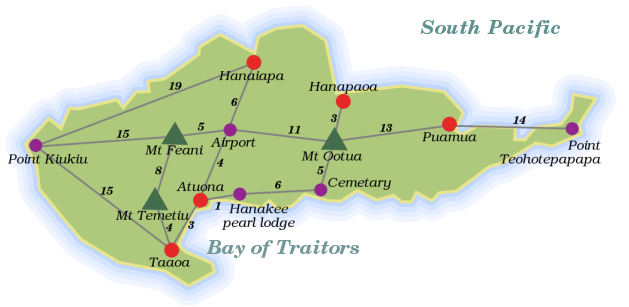
\includegraphics{img/Hiva Oa.png}
\caption{}
\end{figure}

Les lignes grises sont des routes, et les nombres à côté représentent la
longueur de ces routes. Imaginez que l'on ait besoin de connaître le
chemin le plus court pour relier deux endroits sur Hiva Oa. Quelle
approche pourrait-on adopter ?

Non, vraiment, ne lisez pas le paragraphe en diagonale. Essayez de
réfléchir sérieusement aux manières de le faire, et réfléchissez aux
problèmes que vous pourriez rencontrer. Quand vous lisez un livre
technique, il est bien trop facile de parcourir le texte très
rapidement, d'acquiescer solennellement et de s'empresser d'oublier ce
que l'on a lu. Si vous faites sérieusement un effort pour résoudre un
problème, il devient votre problème, et sa solution aura vraiment sens.

\begin{center}\ding{67}\end{center}

Le premier aspect de ce problème est, de nouveau, de représenter nos
informations. Les informations contenues dans l'image n'ont pas beaucoup
de sens pour l'ordinateur. On pourrait essayer de coder un programme qui
étudierait l'image et en extrairait des informations\ldots{} Mais cela
pourrait devenir compliqué. Si on avait vingt milles cartes à
interpréter, ce serait une bonne idée. En l'occurrence, on se chargera
de faire l'interprétation nous-mêmes, et on convertira les données du
plan pour qu'elles soient exploitables en langage informatique.

Que doit savoir notre programme ? Il doit être capable de trouver quel
lieux sont connectés, et quelle distance font les routes qui les
relient. Les lieux et les routes sur l'île forment un graphe, comme les
mathématiciens l'appellent. Il y a plusieurs possibilités pour
enregistrer les graphes. Une solution simple consiste à enregistrer dans
un tableau des objets de type route, chacun étant doté de propriétés
désignant ses deux extrémités et sa longueur.

\begin{lstlisting}
var routes = [{point1: "Point Kiukiu", point2: "Hanaiapa", length: 19},
             {point1: "Point Kiukiu", point2: "Mont Feani", length: 15}
             /* et ainsi de suite */];
\end{lstlisting}
Cependant, il s'avère que lorsque le programme essaiera de déterminer
une route, il aura très souvent besoin de consulter une liste de tous
les routes commençant à un point donné, tout comme une personne qui se
situe à un carrefour aura besoin de regarder les panneaux de direction
et lire «~Hanaiapa : 19 km, Mont Feani : 15 km~». Ce serait sympa si
c'était facile (et rapide) à faire.

Avec la représentation donnée au-dessus, nous devons éplucher tous les
noms de route en gardant ceux qui sont utiles chaque fois que nous
voulons ces panneaux de direction. Une meilleure technique serait
d'enregistrer cette liste directement. Par exemple, utiliser un objet
qui associe les noms de lieux avec la liste des panneaux :

\begin{lstlisting}
var routes = {"Point Kiukiu": [{to: "Hanaiapa", distance: 19},
                              {to: "Mont Feani", distance: 15},
                              {to: "Taaoa", distance: 15}],
             "Taaoa": [/* et cetera */]};
\end{lstlisting}
Quand nous avons cet objet, obtenir les routes qui partent du «~Point
Kiukiu~» revient juste à jeter un œil à
\texttt{routes{[}"Point Kiukiu"{]}}.

\begin{center}\ding{67}\end{center}

Toutefois, cette nouvelle représentation contient des données dupliquées
: la route reliant A à B est listée à la fois dans A et dans B. La
première représentation demandait déjà beaucoup de travail pour rentrer
les données, avec celle-là c'est encore pire.

Heureusement, nous avons à notre disposition le talent de notre
ordinateur pour la répétition des tâches. On peut indiquer les routes
une fois, et faire générer par l'ordinateur la bonne structure de
données. D'abord, définissez un objet initial vide appelé
\texttt{routes}, et écrivez une fonction \texttt{ajouterRoute} :

\begin{lstlisting}
var routes = {};
function creerRoute(depart, arrivee, distance) {
  function ajouterRoute(depart, arrivee) {
    if (!(depart in routes))
      routes[depart] = [];
    routes[depart].push({arrivee: arrivee, distance: distance});
  }
  ajouterRoute(depart, arrivee);
  ajouterRoute(arrivee, depart);
}
\end{lstlisting}
Sympa, n'est-ce pas ? Remarquez comment la fonction interne
(\texttt{ajouterRoute}) utilise les mêmes noms (\texttt{depart} et
\texttt{arrivee}) pour ses paramètres que ceux de la fonction externe.
Ils ne vont pas interférer : à l'intérieur de \texttt{ajouterRoute}, ils
corresdpondent aux paramètre de \texttt{ajouterRoute}, et à l'extérieur,
ils correspondent aux paramètres de \texttt{creerRoute}.

L'instruction \texttt{if} dans \texttt{ajouterRoute} s'assure qu'il y a
un tableau de destinations associées avec le lieu nommé par
\texttt{depart}, et s'il n'y en a pas encore, il ajoute une entrée vide.
De cette façon, à la ligne suivante il peut supposer que le tableau
existe déjà et entrer la nouvelle route dedans.

Maintenant, les informations de la carte ressemblent à ceci :

\begin{lstlisting}
creerRoute("Point Kiukiu", "Hanaiapa", 19);
creerRoute("Point Kiukiu", "Mont Feani", 15);
creerRoute("Point Kiukiu", "Taaoa", 15);
// ...
\end{lstlisting}
\begin{center}\ding{67}\end{center}

Ex. 7.1

Dans la description ci-dessus, on a encore trois fois l'occurrence de la
chaîne de caractères \texttt{"Point Kiukiu"} à la suite. Nous pourrions
générer une description encore plus succincte en permettant à des routes
multiples d'être définies sur une seule ligne.

Écrivez une fonction \texttt{creerRoutes} qui accepte un nombre variable
d'arguments. Le premier argument est toujours le point de départ des
routes, et chaque paire d'arguments qui suit donne le point d'arrivée et
une distance.

Ne dupliquez pas la fonctionnalité de \texttt{creerRoute}, mais demandez
à \texttt{creerRoutes} d'appeler \texttt{creerRoute} pour réaliser la
véritable création de route.

\begin{lstlisting}
function creerRoutes(depart) {
  for (var i = 1; i < arguments.length; i += 2)
    creerRoute(depart, arguments[i], arguments[i + 1]);
}
\end{lstlisting}
Cette fonction utilise un paramètre nommé, \texttt{depart}, et récupère
les autres paramètres dans le (presque-) tableau \texttt{arguments} .
\texttt{i} démarre à \texttt{1} car il doit ignorer le premier
paramètre. \texttt{i += 2} est la simplification de l'équation
\texttt{i = i + 2}, comme vous vous rappelez sans doute.

\begin{lstlisting}
var routes = {};
creerRoutes("Point Kiukiu", "Hanaiapa", 19,
          "Mont Feani", 15, "Taaoa", 15);
creerRoutes("Airport", "Hanaiapa", 6, "Mont Feani", 5,
          "Atuona", 4, "Mont Ootua", 11);
creerRoutes("Mont Temetiu", "Mont Feani", 8, "Taaoa", 4);
creerRoutes("Atuona", "Taaoa", 3, "Hanakee pearl lodge", 1);
creerRoutes("Cemetery", "Hanakee pearl lodge", 6, "Mont Ootua", 5);
creerRoutes("Hanapaoa", "Mont Ootua", 3);
creerRoutes("Puamua", "Mont Ootua", 13, "Point Teohotepapapa", 14);

show(routes["Airport"]);
\end{lstlisting}
\begin{center}\ding{67}\end{center}

Nous avons réussi à réduire considérablement notre description des
informations sur les routes en définissant quelques opérations
pratiques. On pourrait dire que nous avons exprimé l'information de
façon plus succincte en élargissant notre vocabulaire. Définir un `petit
langage' comme ceci est une technique très puissante --- quand, à tout
moment, vous vous retrouvez à écrire du code répétitif et inutile,
arrêtez-vous et essayez de réduire ce code avec du vocabulaire qui le
raccourcira et le condensera.

Le code redondant est non seulement ennuyeux à écrire mais aussi
potentiellement générateur d'erreurs. Les gens font moins attention
quand ils font des choses qui ne requiert pas de la réflexion de leur
part. En plus de cela, le code répétitif est dur à modifier, parce
qu'une structure, qui répète le même motif un millier de fois, doit
également être modifiée un millier de fois si elle s'avère incorrecte ou
suboptimale.

\begin{center}\ding{67}\end{center}

Si vous exécutez tous les morceaux de code ci-dessus, vous devriez avoir
une variable nommée \texttt{routes} qui contient toutes les routes de
l'île. Quand nous avons besoin de la liste des routes qui partent d'un
certain lieu, nous pouvons juste faire \texttt{routes{[}lieu{]}}. Mais
alors, si quelqu'un fait une coquille dans le nom d'un endroit, ce qui
est fort probable avec des noms pareils, il récupèrera un
\texttt{undefined} à la place du tableau qu'il attendait, et des erreurs
étranges peuvent survenir. À la place, nous allons utiliser une fonction
qui permet de récupérer les tableaux de routes et qui nous hurle dessus
si nous lui donnons un nom de lieu inconnu :

\begin{lstlisting}
function routesDepuis(lieu) {
  var trouve = routes[lieu];
  if (trouve == undefined)
    throw new Error("Auncun lieu nommé '" + lieu + "' n'a été trouvé.");
  else
    return trouve;
}

show(routesDepuis("Puamua"));
\end{lstlisting}
\begin{center}\ding{67}\end{center}

Voici un premier jet pour un algorithme de recherche de chemin, la
méthode du joueur :

\begin{lstlisting}
function routeDuJoueur(depart, arrivee) {
  function entierAuHasard(seuil) {
    return Math.floor(Math.random() * seuil);
  }
  function directionAuHasard(depart) {
    var options = routesDepuis(depart);
    return options[entierAuHasard(options.length)].arrivee;
  }

  var chemin = [];
  while (true) {
    chemin.push(depart);
    if (depart == arrivee)
      break;
    depart = directionAuHasard(depart);
  }
  return chemin;
}

show(routeDuJoueur("Hanaiapa", "Mont Feani"));
\end{lstlisting}
À chaque branche de la route, le joueur lance son dé pour décider quelle
route il va prendre. Si le dé le renvoie à son lieu de départ, ainsi
soit-il. Tôt ou tard, il arrivera à destination, du moment que tous les
endroits de l'île sont connectés par des routes.

La ligne la plus déroutante est surement celle contenant
\texttt{Math.random}. Cette fonction renvoie un nombre
pseudo-aléatoire\footnote{Les ordinateurs sont des machines déterministes : elles réagissent tout le temps de la même manière aux données qu'elles reçoivent, et ne peuvent pas produire de réelles valeurs aléatoires. Par conséquent, nous devons nous accommoder d'une série de nombres qui semblent aléatoires, mais qui dans les faits sont le résultat de quelques calculs complexes et déterministes.} entre 0 et 1. Essayez de l'appeler un certain nombre de fois à la console, vous verrez qu'il vous donnera (fort probablement) un nombre différent à chaque fois. La fonction
\texttt{randomInteger} multiplie ce nombre par l'argument qui lui est donné et arrondie le résultat au chiffre inférieur avec
\texttt{Math.floor}. Ainsi par exemple, \texttt{entierAuHasard(3)}
renverra les chiffres \texttt{0}, \texttt{1} ou \texttt{2}.

\begin{center}\ding{67}\end{center}

La méthode du joueur est la manière de faire pour ceux qui abhorrent la
structuration et la planification, qui cherchent désespéremment
l'aventure. Nous avons décidé d'écrire un programme qui peut trouver le
chemin \emph{le plus court} pour aller d'un point à un autre, il nous
faut donc utiliser une autre méthode.

Une approche très simple est de résoudre un tel problème par la méthode
dite «~essais et erreurs~». Il faut :

\begin{enumerate}
\item
  Générer toutes les routes possibles.
\item
  Dans cet ensemble, trouver le plus court chemin qui connecte le point
  de départ au point d'arrivée.
\end{enumerate}
L'étape 2 n'est pas difficile. L'étape 1 est un peu plus problématique.
Si vous acceptez des routes avec des boucles, il existe une infinité de
routes. Bien sûr, il est peu probable que les routes avec des boucles
soient les chemins les plus courts pour aller d'un point à un autre, et
les routes qui ne commencent pas au point de départ ne doivent pas non
plus être prises en compte. Pour un petit graphe telle que Hiva Oa, il
devrait être possible de générer des routes non cycliques (exemptes de
boucles) démarrant d'un lieu donné.

\begin{center}\ding{67}\end{center}

Mais d'abord, nous avons besoin de nouveaux outils. Le premier est une
fonction nommée \texttt{member}, qui est utilisée pour déterminer si un
élément est présent dans un tableau. L'itinéraire (que l'on appellera
également route par la suite) sera conservé comme un tableau de noms, et
quand le voyageur arrivera à un nouveau lieu, l'algorithme appellera
\texttt{member} pour vérifier si le voyageur est déjà passé par cet
endroit. Cela peut ressembler à ça :

\begin{lstlisting}
function member(tableau, valeur) {
  var trouve = false;
  forEach(tableau, function(element) {
    if (element === valeur)
      trouve = true;
  });
  return trouve;
}

print(member([6, 7, "Bordeaux"], 7));
\end{lstlisting}
Toutefois, ceci va parcourir la totalité du tableau, même si la valeur
est trouvée immédiatement en première position. Quel gâchis. Quand vous
utilisez une boucle \texttt{for}, vous pouvez en sortir avec
l'instruction \texttt{break}, mais dans une structure \texttt{forEach}
ceci ne fonctionnera pas, parce que le cœur de la boucle est une
fonction et l'instruction \texttt{break} n'interrompt pas une fonction.
Une solution pour être d'adapter \texttt{forEach} pour qu'il
reconnaissse certains types d'exceptions comme une un signal pour un
arrêt (similaire à \texttt{break} dans les boucles \texttt{for})

\begin{lstlisting}
var Break = {toString: function() {return "Break";}};

function forEach(tableau, action) {
  try {
    for (var i = 0; i < tableau.length; i++)
      action(tableau[i]);
  }
  catch (exception) {
    if (exception != Break)
      throw exception;
  }
}
\end{lstlisting}
\begin{center}\ding{67}\end{center}

Maintenant, si la fonction \texttt{action} lance un \texttt{Break},
\texttt{forEach} absorbera l'exception et interrompra la boucle. L'objet
stocké dans la variable \texttt{Break} est utilisé exclusivement comme
un élément de comparaison. La seule raison pour laquelle je lui ai donné
une propriété \texttt{toString} est qu'il pourrait être très utile de
trouver à quelle étrange valeur vous avez à faire si vous finissez par
récupérer une exception \texttt{Break} en-dehors d'un \texttt{forEach}.

\begin{center}\ding{67}\end{center}

Disposer d'un moyen de sortir de boucles \texttt{forEach} peut être très
utile, mais dans le cas de la fonction \texttt{member} le résultat
demeure assez moche, parce que vous avez besoin de stocker ce résultat
particulier et de le retourner plus tard. Nous pourrions encore ajouter
une autre sorte d'exception, \texttt{Return}, à laquelle on peut
attribuer une propriété \texttt{value}, et faire en sorte que
\texttt{forEach} renvoie cette valeur lorsqu'une exception de ce genre
est lancée, mais ce serait vraiment spécifique à notre problème et
plutôt confus. Ce dont nous avons vraiment besoin c'est d'une nouvelle
fonction de haut niveau, appelée \texttt{any} (ou quelquefois
\texttt{some}). Elle ressemble à ceci :

\begin{lstlisting}
function any(test, tableau) {
  for (var i = 0; i < tableau.length; i++) {
    var trouve = test(tableau[i]);
    if (trouve)
      return trouve;
  }
  return false;
}

function member(tableau, valeur) {
  return any(partial(op["==="], valeur), tableau);
}

print(member(["Peur", "Répugnance"], "Rejet"));
\end{lstlisting}
\texttt{any} parcourt tous les éléments d'un tableau, de gauche à
droite, et les soumet à une fonction de test. La première fois qu'elle
renvoie une valeur comme \texttt{true}, cette valeur est renvoyée.
Sinon, elle retourne \texttt{false}. Appeler \texttt{any(test, tableau)}
est plus ou moins équivalent à
\texttt{test(tableau{[}0{]}) \textbar{}\textbar{} test(tableau{[}1{]}) \textbar{}\textbar{} \ldots{}}
et cætera.

\begin{center}\ding{67}\end{center}

Tout comme \texttt{\&\&} est le pendant de
\texttt{\textbar{}\textbar{}}, \texttt{any} a son pendant, appelé
\texttt{every}:

\begin{lstlisting}
function every(test, tableau) {
  for (var i = 0; i < tableau.length; i++) {
    var trouve = test(tableau[i]);
    if (!trouve)
      return trouve;
  }
  return true;
}

show(every(partial(op["!="], 0), [1, 2, -1]));
\end{lstlisting}
\begin{center}\ding{67}\end{center}

Une autre fonction dont nous aurons besoin est \texttt{flatten}. Cette
fonction prend un tableau de tableaux et met les éléments des tableaux
dans un unique grand tableau.

\begin{lstlisting}
  function flatten(tableaux) {
    var resultat = [];
    forEach(tableaux, function (tableau) {
      forEach(tableau, function (element){resultat.push(element);});
    });
    return resultat;
  }
\end{lstlisting}
La même chose pourrait être faite en utilisant la méthode
\texttt{concat} et un genre de \texttt{reduce}, mais ceci serait moins
efficace. De la même manière, concaténer ensemble des chaînes de
caractères à de nombreuses reprises est plus lent que les mettre dans un
tableau puis appeler la méthode \texttt{join}. Concaténer ensemble des
tableaux de manière répétée produit beaucoup de tableaux intermédiaires
et inutiles.

\begin{center}\ding{67}\end{center}

Ex. 7.2

Avant de commencer à générer des routes, nous avons besoin d'une
fonction d'ordre supérieur supplémentaire. Celle-ci est appelée
\texttt{filter}. Tout comme \texttt{map}, elle prend une fonction et un
tableau en arguments, et produit un nouveau tableau, mais au lieu de
placer le résultat de la fonction appelée dans le nouveau tableau, elle
produit un tableau avec seulement les valeurs de l'ancien tableau pour
lequel la fonction donnée retourne \texttt{true} (ou une valeur
considérée équivalente a \texttt{true}). Écrivez cette fonction.

\begin{lstlisting}
function filter(test, tableau) {
  var resultat = [];
  forEach(tableau, function (element) {
    if (test(element))
      resultat.push(element);
  });
  return resultat;
}

show(filter(partial(op[">"], 5), [0, 4, 8, 12]));
\end{lstlisting}
(Si le résultat de cette utilisation de \texttt{filter} vous surprend,
souvenez-vous que l'argument donné à \texttt{partial} est utilisé comme
le \emph{premier} argument de la fonction, de manière à ce qu'il finisse
à la gauche de \texttt{\textgreater{}}.)

\begin{center}\ding{67}\end{center}

Imaginez à quoi un algorithme permettant de générer des itinéraires
pourrait ressembler --- il commence au point de départ et génére un
itinéraire pour chaque route qui quitte ce lieu. À la fin de chaque
route, il continue à générer des itinéraires supplémentaires. Il ne
parcourt pas un simple itinéraire, il se ramifie. À cause de cela, la
récursion est une manière normale de modéliser ce phénomène.

\begin{lstlisting}
function itinerairesPossibles(depart, arrivee) {
  function trouverItineraires(itineraire) {
    function pasParcouru(route) {
      return !member(itineraire.lieux, route.arrivee);
    }
    function continueItineraire(route) {
      return trouverItineraires({lieux: itineraire.lieux.concat([route.arrivee]),
                         length: itineraire.length + route.distance});
    }

    var fin = itineraire.lieux[itineraire.lieux.length - 1];
    if (fin == arrivee)
      return [itineraire];
    else
      return flatten(map(continueItineraire, filter(pasParcouru,
                                               routesDepuis(fin))));
  }
  return trouverItineraires({lieux: [depart], length: 0});
}

show(itinerairesPossibles("Point Teohotepapapa", "Point Kiukiu").length);
show(itinerairesPossibles("Hanapaoa", "Mont Ootua"));
\end{lstlisting}
La fonction renvoie un tableau d'objets itinéraire, chacun contenant un
tableau de lieux parcourus par l'itinéraire et une longueur.
\texttt{trouverItineraires} continue un itinéraire récursivement,
renvoyant un tableau avec toutes les extensions possibles de cette
route. Quand la fin de l'intinéraire est le lieu défini comme lieu de
fin, il retourne juste l'itinéraire, sachant que continuer l'itinéraire
serait absurde. Si c'est un autre lieu, il faut donc continuer. La ligne
contenant \texttt{flatten}/\texttt{map}/\texttt{filter} est probablement
la plus dure à appréhender. Voilà ce qu'elle dit : «~Prend toutes les
routes partant de ce lieu, en te débarrassant de celles qui vont à des
endroits que nous avons déjà visités. Continue chacune de ces routes, ce
qui donnera pour chacune d'entre elles un tableau d'itinéraires finis,
puis met toutes ces routes dans un grand tableau renvoyé en résultat~».

Cette ligne fait beaucoup de choses. C'est pourquoi une bonne
abstraction de la chose peut aider : elle vous permet de dire des choses
compliquées sans taper un écran entier de code.

Ceci ne risque-t-il pas de se répéter indéfiniment, en continuant à
s'appeler lui-même (via \texttt{continueItineraire}) ? Non, à un certain
moment, toutes les routes iront à des lieux déjà traversés par
l'itinéraire, et le résultat de \texttt{filter} sera un tableau vide.
Cartographier un tableau vide renvoie un tableau vide, l'écraser renvoie
également un tableau vide. Donc appeler \texttt{trouverItineraires} dans
une impasse entraîne un tableau vide, qui signifie «~il n'y a aucun
moyen de continuer cet itinéraire~».

Veuillez noter que les lieux sont ajoutés à des itinéraires en utilisant
\texttt{concat} et non \texttt{push}. La méthode \texttt{concat} crée un
nouveau tableau, alors que \texttt{push} modifie le tableau existant.
Parce que cette fonction risque de faire bifurquer divers itinéraires à
partir d'une seule portion de route, il ne faut pas modifier le tableau
qui représente l'itinéraire original, parce qu'il doit être utilisé
plusieurs fois.

\begin{center}\ding{67}\end{center}

Ex. 7.3

Maintenant que nous avons toutes les itinéraires possibles, essayons de
trouver le plus court. Écrivez une fonction
\texttt{itineraireLePlusCourt} qui, tout comme
\texttt{itinerairesPossibles}, prend les noms des lieux de début et de
fin en arguments. Elle retournera un simple objet itinéraire, du même
type que ce que \texttt{itinerairesPossibles} produit.

\begin{lstlisting}
function itineraireLePlusCourt(depart, arrivee) {
  var itineraireLePlusCourtTrouve = null;
  forEach(itinerairesPossibles(depart, arrivee), function(itineraire) {
    if (!itineraireLePlusCourtTrouve || itineraireLePlusCourtTrouve.length > itineraire.length)
      itineraireLePlusCourtTrouve = itineraire;
  });
  return itineraireLePlusCourtTrouve;
}
\end{lstlisting}
Le point épineux dans les algorithmes de «~minimisation~» ou de «
maximisation~» est qu'il ne faut pas tout massacrer quand un tableau
vide est passé à un tel algorithme. Dans notre cas, on sait qu'il y aura
au moins une route entre 2 lieux donnés, donc nous pouvons simplement
ignorer ce problème. Mais ce raisonnement est un peu léger. Que faire si
la route entre Puamua et le Mont Ootua, qui est escarpée et boueuse, est
emportée par une pluie torrentielle ? Ce serait dommage que cela
engendre une erreur dans notre fonction, donc il faut que la fonction
renvoie une valeur \texttt{null} quand aucun itinéraire n'est trouvé.

Voici donc une approche très ``programmation fonctionnelle'', aussi
abstraite que possible :

\begin{lstlisting}
function minimise(func, tableau) {
  var plusPetitScore = null;
  var trouve = null;
  forEach(tableau, function(element) {
    var score = func(element);
    if (plusPetitScore == null || score < plusPetitScore) {
      plusPetitScore = score;
      trouve = element;
    }
  });
  return trouve;
}

function getProperty(nomDePropriete) {
  return function(objet) {
    return objet[nomDePropriete];
  };
}

function itineraireLePlusCourt(depart, arrivee) {
  return minimise(getProperty("length"), itinerairesPossibles(depart, arrivee));
}
\end{lstlisting}
Malheureusement, cette version est trois fois plus longue que l'autre.
Dans les programmes où vous voulez minimiser un certain nombre de
choses, il peut être intéressant d'écrire un algorithme générique comme
celui-ci, que vous pourrez réutiliser. Dans la plupart des cas, la
première version suffira.

Notez toutefois la fonction \texttt{getProperty}, elle est souvent utile
quand on fait de la programmation fonctionnelle avec des objets.

\begin{center}\ding{67}\end{center}

Voyons à quel trajet aboutit notre algorithme entre la pointe Kiukiu et
la pointe Teohotepapapa\ldots{}

\begin{lstlisting}
show(itineraireLePlusCourt("Point Kiukiu", "Point Teohotepapapa").lieux);
\end{lstlisting}
\begin{center}\ding{67}\end{center}

Sur une petite île comme Hiva Oa, ce n'est pas une tâche insurmontable
de générer tous les itinéraires possibles. Si vous essayez de faire ça
sur une carte raisonnablement détaillée de la Belgique, par exemple,
cela va prendre un temps ridiculement long, sans parler d'une quantité
de mémoire démentielle. Pourtant, vous avez sans doute déjà vu de tels
planificateurs d'itinéraires en ligne. Ils vous indiquent un trajet plus
ou moins idéal parmi un énorme labyrinthe de routes possibles en
quelques secondes à peine. Comment font-ils ça ?

Si vous êtes attentif, vous avez peut-être remarqué qu'il n'est pas
nécessaire de générer tous les itinéraires jusqu'au bout. Si nous
comparons les itinéraires \emph{pendant} que nous les élaborons, nous
pouvons cesser le calcul de ces itinéraires et dès que nous avons trouvé
un premier itinéraire pour notre destination, nous pouvons cesser
l'extension des autres itinéraires plus longs que celui-ci.

\begin{center}\ding{67}\end{center}

Pour essayer, nous utiliserons une grille de 20 sur 20 en guise de carte
:

\begin{figure}[ht!]
\centering
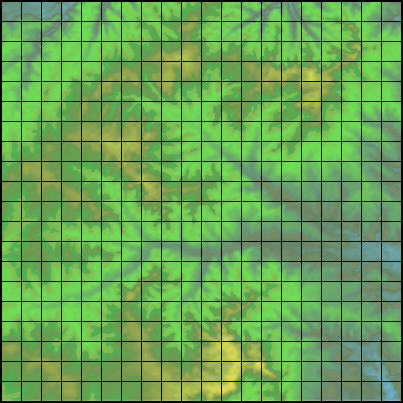
\includegraphics{img/height.png}
\caption{}
\end{figure}

Ce que vous voyez là est une carte en relief d'un terrain montagneux.
Les points jaunes représentent les pics, et les zones bleues, les
vallées. La zone est divisée en carrés de 100 mètres de côté. Nous
disposons d'une fonction \texttt{altitudeEn}, qui peut nous donner
l'altitude en mètres, de n'importe quel carré de cette carte, dans
laquelle les carrés sont représentés par des objets avec des propriétés
\texttt{x} et \texttt{y}.

\begin{lstlisting}
print(altitudeEn({x: 0, y: 0}));
print(altitudeEn({x: 11, y: 18}));
\end{lstlisting}
\begin{center}\ding{67}\end{center}

Nous voulons traverser ce territoire à pied, en partant en haut à gauche
pour arriver en bas à droite. Une grille peut être assimilée à un
graphe. Chaque carré est un nœud connecté aux carrés qui l'entourent.

Nous n'aimons pas gaspiller l'énergie, donc nous préférons prendre le
chemin le plus facile. Monter est plus pénible que descendre, et
descendre plus pénible que marcher sur un terrain
plat\footnote{Si si, je vous assure.}. Cette fonction calcule le «~dénivelé~» entre
deux carrés adjacents, qui représente l'intensité de la fatique que vous
éprouvez à marcher ou grimper de l'un à l'autre. On considère que monter
est deux fois plus pénible que descendre.

\begin{lstlisting}
function distancePonderee(pointA, pointB) {
  var differenceHauteur = altitudeEn(pointB) - altitudeEn(pointA);
  var facteurElevation = (differenceHauteur < 0 ? 1 : 2);
  var distanceaPlat = (pointA.x == pointB.x || pointA.y == pointB.y ? 100 : 141);
  return distanceaPlat + facteurElevation * Math.abs(differenceHauteur);
}
\end{lstlisting}
Notez le calcul de \texttt{distanceaPlat}. Si les deux points sont sur
la même ligne ou colonne, ils sont contigus, et la distance qui les
sépare est cent mètres. Sinon, on considère qu'ils sont adjacents en
diagonale, et la distance en diagonale entre deux carrés de cette taille
est cent fois la racine carrée de deux, ce qui fait à peu près
\texttt{141}. Cette fonction n'est pas autorisée à être appelée pour des
carrés qui sont éloignés de plus d'une unité (elle pourrait faire une
double vérification \ldots{} mais elle est trop paresseuse).

\begin{center}\ding{67}\end{center}

Les points sur la carte sont représentés par des objets contenant des
propriétés \texttt{x} et \texttt{y}. Ces trois fonctions sont utiles
quand on travaille sur de tels objets :

\begin{lstlisting}
function point(x, y) {
  return {x: x, y: y};
}

function ajouterPoints(a, b) {
  return point(a.x + b.x, a.y + b.y);
}

function pointsIdentiques(a, b) {
  return a.x == b.x && a.y == b.y;
}

show(pointsIdentiques(ajouterPoints(point(10, 10), point(4, -2)),
               point(14, 8)));
\end{lstlisting}
\begin{center}\ding{67}\end{center}

Ex. 7.4

Si nous nous mettons à chercher des trajets sur cette carte, nous aurons
encore besoin de créer des «~panneaux~», des listes de directions que
l'on peut prendre à un point donné. Écrivez une fonction
\texttt{directionsPossible} qui prend un objet point comme argument et
renvoie un tableau des points qui l'environnent. Nous pouvons nous
déplacer seulement vers des points adjacents, à la fois en ligne droite
et en diagonale, si bien que les carrés ont au maximum huit carrés
voisins. Prenez garde à ne pas renvoyer des carrés qui se trouveraient
en-dehors de la carte. Pour autant qu'on sache, le bord de la carte
pourrait bien être le bord du monde.

\begin{lstlisting}
function directionsPossible(depart) {
  var dimensionCarte = 20;
  function dansLaCarte(point) {
    return point.x >= 0 && point.x < dimensionCarte &&
           point.y >= 0 && point.y < dimensionCarte;
  }

  var directions = [point(-1, 0), point(1, 0), point(0, -1),
                    point(0, 1), point(-1, -1), point(-1, 1),
                    point(1, 1), point(1, -1)];
  return filter(dansLaCarte, map(partial(ajouterPoints, depart),
                               directions));
}

show(directionsPossible(point(0, 0)));
\end{lstlisting}
J'ai créé une variable \texttt{dimensionCarte}, dans le seul but de ne
pas avoir à écrire deux fois \texttt{20}. Si, à un autre moment, nous
voulons utiliser la même fonction pour une autre carte, ce serait
laborieux avec un code farci de \texttt{20}, qu'il faudrait tous
remplacer un à un. Nous pourrions même aller jusqu'à utiliser
\texttt{dimensionCarte} comme argument de \texttt{directionsPossible},
pour pouvoir utiliser la fonction pour différentes cartes sans les
modifier. J'ai estimé que ce n'était pas nécessaire dans ce cas, de
telles choses peuvent toujours être modifiées quand le besoin s'en fait
sentir.

Alors, pourquoi n'ai-je pas ajouté une variable pour stocker \texttt{0},
qui apparaît également à plusieurs reprises ? J'ai fait comme si les
cartes commençaient toujours à \texttt{0}, donc il est peu probable que
cela change, et utiliser une variable pour cela ne fait qu'ajouter du
bruit.

\begin{center}\ding{67}\end{center}

Pour trouver une route sur cette carte sans que notre navigateur
n'interrompe le programme parce qu'il prend trop de temps à se terminer,
nous devons arrêter de faire de l'amateurisme et mettre en œuvre un
algorithme sérieux. Beaucoup de travail a été consacré à de tels
problèmes dans le passé, et beaucoup de solutions ont été conçues
(certaines brillantes, d'autres inutiles). Une solution très populaire
et efficace est nommé A* (prononcé A étoile). Nous allons consacrer le
reste de ce chapitre à intégrer une fonction de recherche d'itinéraire
A* pour notre carte.

Avant que je me penche sur l'algorithme en lui-même, laissez-moi vous en
dire un peu plus sur le problème qu'il résout. Le problème avec la
recherche de routes par l'intermédiaire de graphes, c'est que dans les
grands graphes, il y a énormément de routes. Notre chercheur de route
Hiva Oa nous a montré que quand le graphe est petit, tout ce que l'on
avait besoin de faire c'était de s'assurer que nos itinéraires ne
repassaient pas par des points où ils étaient déjà passés. Sur notre
nouvelle carte, ceci ne suffit plus.

Le problème fondamental, c'est qu'il y a trop de possibilités pour aller
dans la mauvaise direction. À moins de savoir comment nous diriger vers
la destination pendant l'exploration des chemins, un choix que nous
faisons pour poursuivre une route donnée va plus probablement nous faire
emprunter le mauvais chemin que le bon. Si vous continuez à générer des
itinéraires de cette façon, et même si l'un d'entre eux atteint la cible
de manière accidentelle, vous ne savez pas si c'est le chemin le plus
court.

Donc ce que vous voulez faire, c'est explorer les directions
susceptibles de vous amener à la destination finale en premier. Sur une
grille comme sur une carte, vous pouvez avoir une petite estimation de
l'optimisation d'un tracé en vérifiant sa longueur et la proximité de sa
destination avec la cible. En ajoutant la longueur et l'estimation de la
distance restante, vous pouvez vous faire une bonne idée des itinéraires
qui sont prometteurs. Si vous prolongez les itinéraires prometteurs en
premier, vous avez moins de risques de perdre du temps avec ceux qui
sont inutiles.

\begin{center}\ding{67}\end{center}

Mais cela ne suffit pas encore. Si notre carte était celle d'un monde
parfaitement plat, le chemin qui semble prometteur serait presque
toujours le meilleur, et nous pourrions utiliser la méthode ci-dessus
pour nous rendre directement au but. Mais nous avons des vallées et des
collines sur notre chemin, donc il est difficile de prédire à l'avance
quel itinéraire sera le plus direct. À cause de cela, nous finissons
toujours pas explorer beaucoup trop de possibilités différentes.

Pour y remédier, nous pouvons tirer parti du fait que nous recherchons
sans arrêt l'itinéraire le plus prometteur. Une fois que l'on a
déterminé que le chemin A est le meilleur moyen de se rendre au point X,
nous pouvons nous en souvenir. Quand plus tard le chemin B se rend aussi
au point X, nous savons que ce n'est pas la meilleure route, donc nous
n'avons pas à faire plus de recherches dessus. Ceci peut éviter à notre
programme de tracer beaucoup d'itinéraires inutiles.

\begin{center}\ding{67}\end{center}

Donc, l'algorithme ressemble à quelque chose comme ça :

Il y a deux ensembles de données pour garder un historique. Le premier
est appelé la liste ouverte, elle contient des itinéraires partiels qui
doivent toujours être explorés. Chaque chemin a une note, qui est
calculée en additionnant sa longueur à la distance estimée qui sépare du
but. Cette estimation doit toujours être optimiste, elle ne doit jamais
exagérer la longueur. Le second est un ensemble de nœuds que nous avons
parcouru, avec l'itinéraire partiel qui nous y a amené. Celui-ci, nous
l'appellerons la liste des nœuds atteints. On commence en ajoutant à la
liste ouverte un itinéraire qui contient uniquement le nœud de départ et
on l'enregistre dans la liste des nœuds atteints.

Puis, tant qu'il y a des nœuds dans la liste ouverte, nous prenons celui
qui a le plus petit score (donc le meilleur), et nous trouvons les
directions dans lesquels il peut continuer (en appelant
\texttt{directionsPossible}). Pour chaque nœud obtenu en retour, nous
créons un nouveau chemin en le rattachant à notre route initiale et en
ajustant la longueur du chemin par l'intermédiaire de
\texttt{distancePonderee}. L'extrémité de chacun de ces itinéraires est
ensuite recherchée dans la liste des nœuds atteints.

Si le nœud n'est pas dans la liste des nœuds atteints, cela veut dire
que nous ne l'avons pas encore rencontré avant, nous ajoutons le nouveau
chemin à la liste ouverte, et nous l'enregistrons dans la liste des
nœuds parcourus. Si nous l'\emph{avons} vu avant, nous comparons la note
du nouvel itinéraire aux notes des autres itinéraires de la liste des
nœuds parcourus. Si le nouveau chemin est plus court, on remplace la
route existante avec la nouvelle. Autrement, on se débarrasse du nouvel
itinéraire puisque on a déjà une manière plus rapide de se rendre à ce
point.

On continue ainsi jusqu'à ce que l'itinéraire que nous sortons de la
liste des nœuds parcourus atteigne le nœud correspondant au but ultime,
auquel cas nous avons trouvé notre itinéraire, ou jusqu'à ce que la
liste des nœuds parcourus soit vide, auquel cas nous nous sommes rendus
compte qu'il n'y a pas de route. Dans notre cas, la carte ne contient
pas d'obstacles insurmontables, donc il y a toujours un chemin.

Comment savons-nous que le premier itinéraire complet que nous obtenons
de la liste des nœuds parcourus est le plus direct ? C'est la
conséquence du fait que nous nous intéressons seulement à un chemin
quand il fait le score le plus bas. Le score d'un itinéraire est sa
longueur actuelle additionnée d'un estimation \emph{optimiste} de sa
longueur restante. Cela veut dire que si un itinéraire obtient la note
la plus basse dans la liste ouverte, c'est toujours le chemin le plus
direct vers sa destination finale, c'est impossible pour un autre
itinéraire de trouver plus tard une meilleure route vers ce point, car
si elle était meilleure, son score serait plus bas.

\begin{center}\ding{67}\end{center}

Essayez de ne pas vous énerver lorsque les subtilités de ce
fonctionnement vous échappent. Quand on réfléchit à des algorithmes tels
que ceux là, avoir vu avant «~quelque chose qui y ressemble~» aide
beaucoup, cela vous donne un point de repère pour comparer les
approches. Les programmeurs débutants doivent faire sans de tels points
de repères, ce qui peut les amener facilement à s'égarer. Ayez
simplement conscience que ce travail est d'un niveau assez avancé,
faites une lecture globale du reste du chapitre, et revenez-y plus tard
quand vous vous sentirez de taille à relever le défi.

\begin{center}\ding{67}\end{center}

Je suis désolé de vous l'annoncer, mais pour une partie de l'algorithme,
je vais encore devoir invoquer la magie. La liste ouverte nécessite de
pouvoir disposer d'une grande quantité de routes, et de trouver
rapidement celle qui fait le plus petit score. Les enregistrer dans un
tableau normal et parcourir ce tableau chaque fois est beaucoup trop
lent, je vous donne donc une structure de données appelée tas binaire.
Vous les créez avec \texttt{new}, tout comme les objets \texttt{Date},
en leur donnant une fonction qui est utilisée pour «~donner un score~»
aux éléments passés en argument. L'objet résultant possède les méthodes
\texttt{push} et \texttt{pop}, tout comme un tableau, mais \texttt{pop}
donne toujours l'élément avec le plus petit score, au lieu de donner
celui qui a été ajouté (avec la méthode \texttt{push}) en dernier.

\begin{lstlisting}
function identity(x) {
  return x;
}

var tasBinaire = new BinaryHeap(identity);
forEach([2, 4, 5, 1, 6, 3], function(nombre) {
  tasBinaire.push(nombre);
});
while (tasBinaire.size() > 0)
  show(tasBinaire.pop());
\end{lstlisting}
L'\href{appendix2.html}{appendice 2} traite de l'implémentation de la
structure de données, ce qui est assez intéressant. Après avoir lu le
\href{chapter8.html}{chapitre 8}, vous pourriez vouloir jeter un œil
dessus.

\begin{center}\ding{67}\end{center}

Les nécessités de l'optimisation peut avoir un autre effet. L'algorithme
d'Hiva Oa utilisait des tableaux de destination pour enregistrer les
routes, et copiait celles-ci avec la méthode \texttt{concat} quand il
allongeait ces routes. Cette fois, nous ne pouvons pas nous permettre de
copier des tableaux puisque nous explorerons des tonnes de chemins. À la
place, nous allons utiliser une «~chaîne~» d'objets pour stocker une
route. Chaque objet dans la chaîne possède des propriétés, notamment la
position sur la carte et la longueur de la route déjà effectuée, mais
garde également en mémoire une propriété qui pointe vers l'objet
précédent de la chaîne. Ça donne quelque chose comme ça :

\begin{figure}[ht!]
\centering
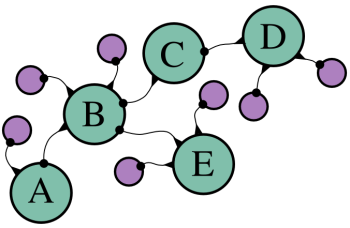
\includegraphics{img/objectchain.png}
\caption{}
\end{figure}

Les cercles couleur cyan sont les objet utiles, et les lignes sont les
propriétés. L'objet \texttt{A} est le début de la route ici. L'objet
\texttt{B} est utilisé pour construire un nouveau tracé qui se prolonge
après \texttt{A}. Quand on doit plus tard reconstruire une route, on
peut se reposer sur ces propriétés pour trouver tous les points par où
la route est passée. On remarque que l'objet \texttt{B} appartient à
deux routes, une qui se termine en \texttt{D}, et une autre qui se
termine en \texttt{E}. Quand il y a beaucoup de routes, cela peut nous
sauver beaucoup d'espace mémoire, chaque nouvelle route nécessite
seulement un nouvel objet pour elle même, le reste est partagé avec les
autres routes qui ont commencé de la même manière.

\begin{center}\ding{67}\end{center}

Ex. 7.5

Écrivez une fonction \texttt{distanceEstimee} qui donne une estimation
optimiste de la distance séparant deux emplacements. Elle n'a pas besoin
de s'intéresser aux données d'altitude, mais peut supposer que le
terrain est plat. Rappelez-vous que l'on se déplace seulement tout droit
et en diagonale, et que l'on compte les déplacements en diagonale entre
deux carrés comme valant \texttt{141}.

\begin{lstlisting}
function distanceEstimee(pointA, pointB) {
  var dx = Math.abs(pointA.x - pointB.x),
      dy = Math.abs(pointA.y - pointB.y);
  if (dx > dy)
    return (dx - dy) * 100 + dy * 141;
  else
    return (dy - dx) * 100 + dx * 141;
}
\end{lstlisting}
Ces formules étranges sont utilisées pour décomposer le trajet en une
partie rectiligne et une partie en diagonale. Si vous avec un trajet tel
que celui-là :

\begin{figure}[ht!]
\centering
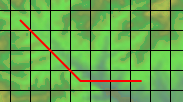
\includegraphics{img/diagonalpath.png}
\caption{}
\end{figure}

\ldots{} le chemin fait \texttt{8} cases de larges et \texttt{4} de
haut, donc vous avez \texttt{8 - 4 = 4} déplacements rectilignes et
\texttt{4} déplacements en diagonales.

Si vous écriviez une fonction qui calcule la distance «~pythagoricienne
» directe entre ces points, cela fonctionnerait aussi. Ce dont nous
avons besoin est d'une estimation optimiste, et supposer que nous
pouvons aller tout droit vers notre but est certainement optimiste. Quoi
qu'il en soit, plus notre estimation est correcte, moins notre programme
essaiera des itinéraires inutiles.

\begin{center}\ding{67}\end{center}

Ex. 7.6

Nous allons utiliser un tas binaire pour stocker la liste ouverte.
Quelle structure serait la bonne pour la liste des nœuds atteints ?
Cette liste sera utilisée pour chercher des routes, en lui passant un
couple \texttt{x}, \texttt{y} de coordonnées. Rapidement de préférence.
Ecrivez trois fonctions \texttt{creerListePointsParcourus},
\texttt{stockerPointsParcourus}, et \texttt{trouverPointsParcourus}. La
première crée la structure de données ; la seconde, étant donnée une
liste de nœuds atteints, un point, et une route, stocke cette route; la
dernière, étant donné une liste de nœuds atteints et un point, retourne
une route ou \texttt{undefined} pour indiquer qu'aucune route n'a été
trouvée pour ce point.

Une idée raisonnable serait d'utiliser un objet avec des objets à
l'intérieur. Une des coordonnées des points, par exemple \texttt{x}, est
utilisé comme nom de propriété pour l'objet extérieur, et l'autre,
\texttt{y}, pour l'objet intérieur. Cela va nécessiter un peu de tenue
de compte pour gérer le fait que, parfois, l'objet intérieur que nous
recherchons n'existe pas (encore).

\begin{lstlisting}
function creerListePointsParcourus() {
  return {};
}

function stockerPointsParcourus(liste, point, itineraire) {
  var listeInterne = liste[point.x];
  if (listeInterne == undefined) {
    listeInterne = {};
    liste[point.x] = listeInterne;
  }
  listeInterne[point.y] = itineraire;
}

function trouverPointsParcourus(liste, point) {
  var listeInterne = liste[point.x];
  if (listeInterne == undefined)
    return undefined;
  else
    return listeInterne[point.y];
}
\end{lstlisting}
Une autre possiblité est de fusionner les \texttt{x} et \texttt{y} du
point en un nom unique de propriété, et de l'utiliser pour stocker les
itinéraires dans un objet unique.

\begin{lstlisting}
function pointID(point) {
  return point.x + "-" + point.y;
}

function creerListePointsParcourus() {
  return {};
}

function stockerPointsParcourus(liste, point, itineraire) {
  liste[pointID(point)] = itineraire;
}

function trouverPointsParcourus(liste, point) {
  return liste[pointID(point)];
}
\end{lstlisting}
\begin{center}\ding{67}\end{center}

Définir un type de structure données en fournissant un ensemble de
fonctions pour créer et manipuler de telles structures est une technique
utile. Cela permet «~d'isoler~» le code qui utilise la structure, des
détails de la structure elle-même. Remarquez que, peu importe laquelle
des deux implémentations ci-dessus est utilisée, le code qui a besoin
d'une liste des nœuds atteints fonctionne exactement de la même façon.
Il ne se préoccupe pas du type d'objet utilisé, tant qu'il reçoit le
résultat qu'il attend.

On discutera plus en détail de cela au \href{chapter8.html}{chapitre 8},
où nous apprendrons à faire des types d'objet comme \texttt{BinaryHeap}
(tas binaire), qui sont créés en utilisant \texttt{new} et qui ont des
méthodes pour les manipuler.

\begin{center}\ding{67}\end{center}

Nous avons donc enfin notre vrai fonction de recherche de chemin :

\begin{lstlisting}
function trouverItineraire(depart, arrivee) {
  var listeOuverte = new BinaryHeap(scoreItineraire);
  var pointsParcourus = creerListePointsParcourus();

  function scoreItineraire(itineraire) {
    if (itineraire.score == undefined)
      itineraire.score = distanceEstimee(itineraire.point, arrivee) +
                    itineraire.longueur;
    return itineraire.score;
  }
  function ajouterItineraireOuvert(itineraire) {
    listeOuverte.push(itineraire);
    stockerPointsParcourus(pointsParcourus, itineraire.point, itineraire);
  }
  ajouterItineraireOuvert({point: depart, longueur: 0});

  while (listeOuverte.size() > 0) {
    var itineraire = listeOuverte.pop();
    if (pointsIdentiques(itineraire.point, arrivee))
      return itineraire;

    forEach(directionsPossible(itineraire.point), function(direction) {
      var itineraireConnu = trouverPointsParcourus(pointsParcourus, direction);
      var nouvelleLongueur = itineraire.longueur +
                      distancePonderee(itineraire.point, direction);
      if (!itineraireConnu || itineraireConnu.longueur > nouvelleLongueur){
        if (itineraireConnu)
          listeOuverte.remove(itineraireConnu);
        ajouterItineraireOuvert({point: direction,
                      from: itineraire,
                      longueur: nouvelleLongueur});
      }
    });
  }
  return null;
}
\end{lstlisting}
Premièrement, il crée les structures de données dont il a besoin : une
liste ouverte et une liste des nœuds atteints. \texttt{scoreItineraire}
est la fonction de calcul de score passée au tas binaire. Remarquez
comment il stocke ses résultats dans l'objet route, pour éviter d'avoir
à le recalculer plusieurs fois.

\texttt{ajouterItineraireOuvert} est une fonction commode pour ajouter
une nouvelle route à la fois à la liste ouverte et à la liste des nœuds
atteints. On l'utilise immédiatement pour ajouter le début de la route.
Remarquez que les objets route ont roujours une propriétés
\texttt{point}, qui stocke le point d'arrivée de la route, et
\texttt{longueur}, qui stocke la longueur courante de la route. Les
routes qui ont plus d'une case de longueur, ont aussi une propriété
\texttt{depart}, qui pointe sur leurs prédécesseurs.

La boucle \texttt{while}, comme décrit dans l'algorithme, prend
constamment la route de plus faible score dans la liste ouverte et
vérifie si cela nous mène au but. Si ce n'est pas le cas, on doit
continuer en l'étendant. C'est ce dont s'occupe \texttt{forEach}. Il
cherche si ce nouveau point est dans la liste des nœuds atteints. S'il
ne le trouve pas, ou si le nœud trouvé a une route plus longue que la
nouvelle route, un nouveau objet route est créé et ajouté à la liste
ouverte et la liste des nœuds atteints, et la route existante (s'il y en
a une) est supprimée de la liste ouverte.

Que se passe-t-il si la route dans \texttt{itineraireConnu} n'est pas
dans la liste ouverte ? Cela peut arriver, car les routes ne sont
supprimés de la liste ouverte que lorsqu'on a déterminé qu'elles étaient
la route optimale pour atteindre leur destination. Si nous essayons de
supprimer du tas binaire, une valeur qui n'y ait pas, cela va lever une
exception, donc si mon raisonnement est faux, nous verrons probablement
un exception au moment d'exécuter la fonction.

Quand le code devient suffisamment complexe pour vous faire douter de
certaines choses à son propos, c'est une bonne idée d'ajouter quelques
vérifications qui lèvent une exception quand quelque chose se passe mal.
De cette façon, vous savez qu'il ne se passe rien de bizarre «
silencieusement~», et quand vous cassez quelque chose, vous saurez
immédiatement ce que vous avez cassé.

\begin{center}\ding{67}\end{center}

Remarquez que cette algorithme n'utilise pas la récursion, mais réussit
quand même à explorer toutes les branches. La liste ouverte remplace
plus ou moins le rôle qu'avait la pile d'appel de fonction dans la
solution récursive du problème Hiva Oa : il garde une trace des chemins
qui doivent encore être parcourus. Chaque algorithme récursif peut être
réécrit d'une façon non-récursive et utilisant une structure de données
qui stocke les «~choses encore à faire~».

\begin{center}\ding{67}\end{center}

Bien, essayons notre recherche de route :

\begin{lstlisting}
var route = trouverItineraire(point(0, 0), point(19, 19));
\end{lstlisting}
Si vous avez exécuter tout le code depuis le début du chapitre, et que
vous n'avez pas introduit d'erreurs, cet appel, même si cela peut
prendre quelques secondes à s'exécuter, devrait vous donner un objet
route. Cet objet est plutôt difficile à lire. On peut le faire en
utilisant la fonction \texttt{showRoute} qui, si votre console est assez
grande, vous montrera une route sur une carte.

\begin{lstlisting}
showRoute(route);
\end{lstlisting}
Vous pouvez également passer plusieurs routes à \texttt{showRoute}, ce
qui peut être utile si, par exemple, vous voulez planifier un itinéraire
touristique, qui doit inclure le magnifique point de vue en \texttt{11},
\texttt{17}.

\begin{lstlisting}
showRoute(trouverItineraire(point(0, 0), point(11, 17)),
          trouverItineraire(point(11, 17), point(19, 19)));
\end{lstlisting}
\begin{center}\ding{67}\end{center}

Les variations sur le thème chercher un itinéraire optimal dans un
graphe peut être appliqué à de nombreux problèmes, dont beaucoup ne sont
pas liés au fait de trouver un chemin physique. Par exemple, un
programme qui résout le problème de faire rentrer un nombre donné de
blocs dans un espace limité, peut être résolu en explorant les
différents `chemins' possibles qu'il obtient en essayant de positionner
un certain bloc à une certaine place. Les chemins se terminant avec un
manque de place pour les derniers blocs sont des culs-de-sac, et le
chemin qui permet de faire rentrer tous les blocs dans l'espace est la
solution.


\chapter{Programmation orientée objet}

Au début des années 90, une chose appelée programmation orientée objet
souffla un vent nouveau sur l'industrie du logiciel. La plupart des
idées derrière ce concept n'étaient pas vraiment nouvelles, mais elles
avaient enfin suffisamment d'élan pour décoller, et devenir «~à la mode
». Des livres furent écrits sur le sujet, des cours furent organisés,
des langages de programmation développés. Tout d'un coup, tout le monde
se mit à vanter les mérites de la programmation orientée objet,
appliquant ses recettes à tous les problèmes avec enthousiasme, se
convainquant qu'on avait enfin trouvé \emph{la bonne façon d'écrire des
programmes}.

Ces choses arrivent souvent. Quand un problème est compliqué. Les gens
cherchent toujours une solution magique. Quand arrive quelque chose qui
ressemble à cette solution, ils sont prêts à s'y jeter corps et âme.
Pour de nombreux programmeurs, encore aujourd'hui, l'orientation objet
(ou du moins la vision qu'ils en ont) est la panacée. Si un programme
n'est pas «~en pur objet~», quel que soit le sens de cette expression,
il est considéré comme résolument inférieur.

Toutefois, peu d'engouements ont duré si longtemps. La longévité de la
programmation orientée objet peut sûrement s'expliquer par le fait que
les idées centrales de concept sont utiles et simples. Dans ce chapitre,
nous allons parler de ces idées et de leur application, plutôt
excentrique, au JavaScript. Les paragraphes précédents n'étaient
absolument pas destinés à discréditer ces idées. Mon objectif était
juste d'éviter qu'on ne jure plus que par elles.

\begin{center}\ding{67}\end{center}

Comme son nom l'indique, la programmation orientée objet est centrée sur
la notion d'objet. Depuis le début, nous avons utilisé les objets comme
des espèces de fourre-tout plein de valeurs, où l'on ajoute ou modifie
des propriétés à notre guise. En fait, dans une approche orientée objet,
les objets sont vus comme des microcosmes indépendants, qui ne
communiquent avec l'extérieur qu'à travers un nombre limité
d'interfaces, un ensemble de méthodes et propriétés spécifiques. La «
liste des nœuds atteints~» utilisée à la fin du
\href{chapter7.html}{chapitre 7} en est un exemple : nous avons utilisé
trois fonctions, \texttt{creerListePointsParcourus},
\texttt{stockerPointsParcourus} et \texttt{trouverPointsParcourus} pour
interagir avec elle. Ces trois fonctions forment une interface pour
cette sorte d'objets.

Les objets \texttt{Date}, \texttt{Error} et \texttt{BinaryHeap} que nous
avons vus fonctionnent également comme cela. Au lieu de fournir des
fonctions classiques pour travailler avec ces objets, ils fournissent
une manière d'être créés, via le mot-clé \texttt{new}, et un certain
nombre de méthodes et propriétés qui forment le reste de l'interface.

\begin{center}\ding{67}\end{center}

Pour faire une méthode d'objet, il suffit de définir une variable qui
contiendra une fonction.

\begin{lstlisting}
var lapin = {};
lapin.parler = function(tirade) {
  print("Le lapin dit '", tirade, "'");
};

lapin.parler("Eh bien, maintenant c'est vous qui me le demandez.");
\end{lstlisting}
Dans la plupart des cas, la méthode aura besoin de savoir sur \emph{qui}
elle doit s'appliquer. Par exemple, s'il y a plusieurs lapins, la
méthode \texttt{parler} doit pouvoir indiquer quel est le lapin qui
parle. Pour ce faire, il y a une variable spéciale appelée
\texttt{this}, qui est toujours définie à l'intérieur d'une fonction et
qui pointe vers l'objet sur lequel la fonction s'applique. Une fonction
est appelée comme une méthode quand elle est définie en tant que
propriété d'un objet, et appelée directement comme ceci :
\texttt{objet.methode()}.

\begin{lstlisting}
function parler(tirade) {
  print("Le lapin ", this.adjectif, " dit « ", tirade, " »");
}
var lapinBlanc = {adjectif: "blanc", parler: parler};
var grosLapin = {adjectif: "gras", parler: parler};

lapinBlanc.parler("Par ma moustache et mes oreilles, comme il se fait tard !");
grosLapin.parler("J'ai bien envie d'une carotte, maintenant.");
\end{lstlisting}
\begin{center}\ding{67}\end{center}

Je peux maintenant clarifier la présence du mystérieux premier argument
de la méthode \texttt{apply}, pour lequel nous avons toujours mis
\texttt{null} dans le \href{chapter6.html}{chapitre 6}. Cet argument
peut être utilisé pour spécifier un objet sur lequel la fonction
s'appliquera, qui prendra donc le rôle de \texttt{this}. Toutefois, pour
les fonctions qui ne sont pas des méthodes, cela n'a pas de sens, d'où
le \texttt{null}.

\begin{lstlisting}
parler.apply(grosLapin, ["Miam."]);
\end{lstlisting}
Les fonctions ont également une méthode \texttt{call}, qui se comporte
comme \texttt{apply}, à l'exception du fait que les arguments peuvent
être fournis séparéments, et non dans un tableau :

\begin{lstlisting}
parler.call(grosLapin, "Rot.");
\end{lstlisting}
\begin{center}\ding{67}\end{center}

Le mot-clé \texttt{new} fournit un bon moyen de créer de nouveaux
objets. Quand une fonction est appelée avec le mot \texttt{new} devant,
sa variable \texttt{this} pointe sur un \emph{nouvel} objet, qui sera
automatiquement retourné (à moins que la fonction ne retourne
explicitement autre chose). Les fonctions utilisées pour créer de
nouveaux objets comme ça sont appelées des constructeurs. En voici un
pour les lapins :

\begin{lstlisting}
function Lapin(adjectif) {
  this.adjectif = adjectif;
  this.parler = function(tirade) {
    print("Le lapin ", this.adjectif, " dit '", tirade, "'");
  };
}

var lapinTueur = new Lapin("tueur");
lapinTueur.parler("GRAAAAAAAAAH !");
\end{lstlisting}
Il y a une convention, parmis les programmeurs JavaScript, qui consiste
à faire débuter les noms de constructeurs par une lettre majuscule. Cela
permet de mieux les reconnaîtres au milieu des autres fonctions.

Mais pourquoi le mot clés \texttt{new} est-il nécessaire ? Après tout,
nous aurions pu écrire simplement :

\begin{lstlisting}
function creerLapin(adjectif) {
  return {
    adjectif: adjectif,
    parler: function(tirade) {/*etc.*/}
  };
}

var lapinNoir = creerLapin("noir");
\end{lstlisting}
Mais ce n'est pas exactement la même chose. \texttt{new} en fait
discrètement plus. En fait, notre fonction \texttt{lapinTueur} a une
propriété appelée \texttt{constructor}, qui pointe vers la fonction
\texttt{Lapin} l'ayant créée. \texttt{lapinNoir} a également cette
propriété, mais elle pointe vers la fonction \texttt{Object}.

\begin{lstlisting}
show(lapinTueur.constructor);
show(lapinNoir.constructor);
\end{lstlisting}
\begin{center}\ding{67}\end{center}

D'où vient la propriété \texttt{constructor} ? Elle fait partie du
prototype d'un lapin. Les prototypes sont une partie importante du
fonctionnement des objets en JavaScript. Chaque objet est basé sur un
prototype, qui lui confère un ensemble de propriétés. Les objets simples
que nous avons utilisés jusque là sont tous basés sur le plus
élémentaires des prototypes, celui associé au constructeur
\texttt{Object}. En fait, taper \texttt{\{\}} est équivalent à taper
\texttt{new Object()}.

\begin{lstlisting}
var objetSimple = {};
show(objetSimple.constructor);
show(objetSimple.toString);
\end{lstlisting}
\texttt{toString} est une méthode qui fait partie du prototype
\texttt{Object}. Ça signifie que tous les objets de base ont une méthode
\texttt{toString}, qui les converti en chaîne de caractères. Nos objets
lapin sont basés sur le prototype associé au constructeur
\texttt{Lapin}. Il est possible d'utiliser la propriété
\texttt{prototype} d'un constructeur pour accéder à\ldots{} leur
prototype :

\begin{lstlisting}
show(Lapin.prototype);
show(Lapin.prototype.constructor);
\end{lstlisting}
Chaque fonction est automatiquement munie d'une propriété
\texttt{prototype}, dont la propriété \texttt{constructor} renvoie à la
fonction. Puisque que le prototype «~lapin~» est lui-même un objet, il
est basé sur le prototype \texttt{Object}, et partage sa méthode
\texttt{toString}.

\begin{lstlisting}
show(lapinTueur.toString == objetSimple.toString);
\end{lstlisting}
\begin{center}\ding{67}\end{center}

Même si les objets semblent partager des propriétés avec leur prototype,
ce partage n'est qu'à sens unique. Les propriétés des prototypes
influencent les objets basés dessus, mais les propriétés de cet objet ne
changent jamais le prototype.

Les règles sont précisément les suivantes : pour trouver la valeur d'une
propriété, JavaScript cherche d'abord parmis les propriétés de l'objet
\emph{lui-même}. S'il y a une propriété qui porte le nom de l'on
recherche, c'est sa valeur que l'on obtient. S'il n'y en a pas, la
recherche se poursuit à travers le prototype de l'objet, et ensuite à
travers le prototype du prototype, et ainsi de suite. Si aucune
propriété n'est trouvée, c'est la valeur \texttt{undefined} qui est
renvoyée. À l'inverse, lorsqu'on \emph{défini} la valeur d'une
propriété, JavaScript ne remonte jamais au prototype, il attribue
directement la valeur à une propriété de l'objet lui-même.

\begin{lstlisting}
Lapin.prototype.dents = "petites";
show(lapinTueur.dents);
lapinTueur.dents = "longues, pointues et sanglantes";
show(lapinTueur.dents);
show(Lapin.prototype.dents);
\end{lstlisting}
Cela signifie que le prototype peut être utilisé pour ajouter des
propriétés et des méthodes à tous les objets basés dessus. Par exemple,
il se peut que nos lapins aient soudainement besoin de danser.

\begin{lstlisting}
Lapin.prototype.danser = function() {
  print("Le lapin ", this.adjectif, " danse une jigue.");
};

lapinTueur.danser();
\end{lstlisting}
Et, comme vous vous en doutez, le prototype de lapin est le meilleur
endroit où ajouter des éléments communs à tous les lapins, comme la
méthode \texttt{parler}. Voici donc une nouvelle approche pour notre
constructeur de \texttt{Lapin} :

\begin{lstlisting}
function Lapin(adjectif) {
  this.adjectif = adjectif;
}
Lapin.prototype.parler = function(tirade) {
  print("Le lapin ", this.adjectif, " dit '", tirade, "'");
};

var noisetteLeLapin = new Lapin("noisette");
noisetteLeLapin.parler("Good Frith!");
\end{lstlisting}
\begin{center}\ding{67}\end{center}

Le fait que tous les objets aient leur prototype et reçoivent des
propriétés de ce prototype peut apporter quelques complications. Ça
signifie qu'utiliser un objet pour stocker des trucs, comme les chats du
\href{chapter4.html}{chapitre 4}, peut mal se passer. Par exemple, si
nous nous étions demandé s'il y a un chat nommé «~\texttt{constructor}
», nous aurions implémenté le test suivant :

\begin{lstlisting}
var pasUnSeulChat = {};
if ("constructor" in pasUnSeulChat)
  print("Oui, il y a sans aucun doute un chat appelé « constructor ».");
\end{lstlisting}
C'est problématique. Un autre problème tient au fait qu'il est souvent
pratique d'étendre les prototypes des constructeurs standards comme
\texttt{Object} ou \texttt{Array} avec de nouvelles fonctions. Par
exemple, nous pouvons donner à tous les objets une méthode nommée
\texttt{properties}, qui retourne un tableau contenant le nom des
propriétés (non cachées) d'un objet.

\begin{lstlisting}
Object.prototype.properties = function() {
  var resultat = [];
  for (var property in this)
    resultat.push(property);
  return resultat;
};

var test = {x: 10, y: 3};
show(test.properties());
\end{lstlisting}
Et cela met tout de suite le problème en évidence. Maintenant que le
prototype \texttt{Object} a une propriété appelée \texttt{properties},
parcourir les propriétés de n'importe quel objet, en utilisant
\texttt{for} et \texttt{in}, renverra également cette propriété
partagée, ce qui n'est généralement pas ce que nous souhaitons. Nous
sommes seulement intéressés par les propriétés que l'objet a lui-même.

Heureusement, il y a un moyen de trouver si une propriété appartient à
un objet lui-même, ou à l'un de ses prototypes. Malheureusement, cela
complique un peu le parcours des propriétés d'un objet. Tout objet a une
méthode appelée \texttt{hasOwnProperty}, qui nous indique si l'objet a
une propriété de ce nom. En se basant sur ce mécanisme, nous pouvons
ré-écrire notre méthode \texttt{properties} de la manière suivante :

\begin{lstlisting}
Object.prototype.properties = function() {
  var resultat = [];
  for (var property in this) {
    if (this.hasOwnProperty(property))
      resultat.push(property);
  }
  return resultat;
};

var test = {"Gros Igor": true, "Boule de Feu": true};
show(test.properties());
\end{lstlisting}

Et bien sûr, nous pouvons abstraire cela dans une fonction de haut
niveau. Notez que la fonction \texttt{action} est appelée avec à la fois
le nom de la propriété et la valeur qu'elle a dans l'objet.

\begin{lstlisting}
function forEachIn(objet, action) {
  for (var property in objet) {
    if (objet.hasOwnProperty(property))
      action(property, objet[property]);
  }
}

var chimere = {visage: "lion", corps: "chèvre", derrière: "serpent"};
forEachIn(chimere, function(nom, valeur) {
  print("Un ", nom, " de ", valeur, ".");
});
\end{lstlisting}

Mais, que se passe-t-il si on rencontre un chat nommé
\texttt{hasOwnProperty} ? (on ne sait jamais.) Il sera stocké dans
l'objet, et la tentative suivante de parcourir la collection de chats,
utilisant \texttt{objet.hasOwnProperty}, sera un échec, car cette
propriété ne pointera plus vers la fonction. Une façon d'éviter ce
problème est d'agir encore plus salement :

\begin{lstlisting}
function forEachIn(objet, action) {
   for (var property in objet) {
       if (Object.prototype.hasOwnProperty.call(objet, property))
           action(property, objet[property]);
   }
}

var test = {name: "Mardochée", hasOwnProperty: "Oh-oh"};
forEachIn(test, function (nom, valeur) {
   print ("Property ", nom, " = ", valeur);
});
\end{lstlisting}

(Note : Cet exemple ne fonctionne pas pour l'instant correctement dans
Internet Explorer 8, qui a semble-t-il des problèmes avec la
redéfinition des propriétés intégrées.)

Ici, au lieu d'utiliser la méthode trouvée dans l'objet lui-même, nous
prenons la méthode fournie par le prototype \texttt{Object}, et
l'appliquons en utilisant \texttt{call} sur le bon objet. À moins que
quelqu'un n'ait joué avec la méthode de \texttt{Object.prototype} (et ne
faîtes pas ça), le programme devrait fonctionner correctement.

\begin{center}\ding{67}\end{center}

\texttt{hasOwnProperty} peut également être utilisée dans les situations
où l'on utilise l'opérateur \texttt{in} pour savoir si un objet contient
une propriété particulière. Mais il y a encore une subtilité. Nous avons
vu dans le \href{chapter4.html}{chapitre 4} que certaines propriétés,
comme \texttt{toString}, sont `cachées', et ne sont donc pas considérées
lors du parcours des éléments d'un objet via une instruction
\texttt{for}/\texttt{in}. Il s'avère que les navigateurs de la famille
Gecko (Firefox principalement) donnent à chaque objet une propriété
cachée nommée \texttt{\_\_proto\_\_}, qui pointe vers le prototype de
cet objet. \texttt{hasOwnProperty} retourne \texttt{true}, pour cette
propriété, même si le programme ne l'a pas explicitement ajoutée. Avoir
accès au prototype d'un objet peut être très pratique, mais en faire une
propriété comme ça n'était pas une très bonne idée. Toutefois, Firefox
est un navigateur web très utilisé, et il convient de faire attention à
cela quand vous écrivez des programmes pour le web. Il y a une méthode
\texttt{propertyIsEnumerable}, qui retourne \texttt{false}, pour les
propriétés cachées, et peut donc être utilisé pour filtrer les
étrangetés comme \texttt{\_\_proto\_\_}. Pour contourner ce problème de
manière fiable, on peut utiliser une expression comme :

\begin{lstlisting}
var objet = {foo: "bar"};
show (Object.prototype.hasOwnProperty.call(objet, "foo") &&
   Object.prototype.propertyIsEnumerable.call(objet, "foo"));
\end{lstlisting}
Simple et agréable n'est-ce pas ? C'est l'un des aspects de JavaScript
qui ne sont pas-si-bien-conçus-que-ça. Les objets jouent à la fois le
rôle de «~valeurs avec méthodes~», qui fonctionnent très bien avec les
prototypes, et «~d'ensemble de propriétés~», pour lesquels les
prototypes ne font que déranger.

\begin{center}\ding{67}\end{center}

Écrire l'expression ci-dessus à chaque fois qu'on a besoin de vérifier
la présence d'une propriété dans un objet n'est pas viable. Nous
pourrions le mettre dans une fonction, mais une meilleur approche est
encore d'écrire un constructeur et un prototype dédié aux situations où
nous voulons utiliser un objet simplement comme un ensemble propriétés.
Puisqu'il est prévu pour pouvoir y chercher des choses par leurs noms,
nous l'appellerons \texttt{Dictionary} (dictionnaire).

\begin{lstlisting}
function Dictionary(valeursInitiales) {
  this.valeurs = valeursInitiales || {};
}
Dictionary.prototype.store = function(nom, valeur) {
  this.valeurs[nom] = valeur;
};
Dictionary.prototype.lookup = function(nom) {
  return this.valeurs[nom];
};
Dictionary.prototype.contains = function(nom) {
  return Object.prototype.hasOwnProperty.call(this.valeurs, nom) &&
    Object.prototype.propertyIsEnumerable.call(this.valeurs, nom);
};
Dictionary.prototype.each = function(action) {
  forEachIn(this.valeurs, action);
};

var couleurs = new Dictionary({Grover: "bleu",
                              Elmo: "orange",
                              Bart: "jaune"});
show(couleurs.contains("Grover"));
show(couleurs.contains("constructor"));
couleurs.each(function(nom, couleur) {
  print(nom, " est ", couleur);
});
\end{lstlisting}
Désormais, tous les inconvénients de l'utilisation des objets en tant
qu'ensemble de propriétés sont «~cachés~» derrière une interface
pratique : un constructeur et quatre méthodes. Notez que la propriété
\texttt{valeurs} d'un objet \texttt{Dictionary} ne fait pas partie de
son interface, ce n'est qu'un détail interne, et quand vous utilisez des
objets \texttt{Dictionary}, vous n'avez pas besoin de l'utiliser
directement.

Chaque fois que vous écrivez une interface, il est utile d'y ajouter un
commentaire retraçant rapidement ce qu'elle fait et comment l'utiliser.
De cette manière, quand quelqu'un (éventuellement vous dans trois mois),
souhaite travailler avec cette interface, il peut se faire rapidement
une idée de comment l'utiliser, et n'a alors pas besoin d'étudier tout
le programme.

La plupart du temps, quand vous concevez une nouvelle interface, vous
êtes rapidement confrontés à des problèmes et des limitations dans ce
que vous aviez prévu. En conséquence, vous changez votre interface. Pour
éviter de perdre du temps, il est conseillé de ne documenter vos
interfaces \emph{qu'après} les avoir expérimentées un certain temps sur
des cas concrets, et qu'elles se soient révélées efficaces. -- Bien sûr,
cela pourrait augmenter la tentation de ne pas documenter du tout. Mais
personnellement, je considère la documentation comme une «~touche finale
», à ajouter au système. Quand ça donne l'impression d'être prêt, c'est
qu'il est temps d'écrire un peu sur le sujet, et de voir si ça sonne
aussi bien en français (ou n'importe quelle autre langue vivante), qu'en
JavaScript (où n'importe quel autre langage de programmation).

\begin{center}\ding{67}\end{center}

La distinction entre l'interface d'un objet et ses détails de
fonctionnement internes est importante pour deux raisons. D'abord, avoir
une petite interface bien décrite rend un objet plus facile à utiliser.
Il suffit de garder l'interface en tête, sans plus se préoccuper du
reste, à moins d'avoir à changer l'objet lui-même.

Ensuite, il arrive régulièrement d'avoir à changer quelque chose dans le
fonctionnement interne d'un type\footnote{Ces types sont souvent appelés des «~classes~» dans d'autres langages de programmation.} d'objet, pour le rendre plus efficace par exemple, ou pour corriger un problème. Si le
code extérieur a accès à toutes les propriétés d'un objet, il est
difficile de changer le moindre détail sans avoir à mettre à jour tout
le reste du code. Si le code extérieur utilise une petite interface,
vous pouvez changer le fonctionnement interne de l'objet comme bon vous
semble, tant que l'interface ne change pas.

Certaines personnes vont assez loin avec ce concept. Ils n'incluent, par
exemple, aucune propriété dans l'interface d'un objet, et n'y autorisent
que des méthodes -- si leur type d'objet a une longueur, elle sera
accessible via une méthode \texttt{getLength}, et pas directement comme
une propriété \texttt{length}. De cette manière, si jamais ils décident
de modifier leur objet de telle manière qu'il n'a plus de propriété
\texttt{length}, par exemple parce que la longueur à retourner devient
celle d'un tableau, ils peuvent mettre la fonction à jour, sans changer
l'interface.

D'après mon point de vue personnel, dans la plupart des cas cela n'en
vaut pas la peine. Ajouter une méthode \texttt{getLength} ne contenant
que \texttt{return this.length;} est essentiellement un ajout de code
inutile. En règle générale, je considère le code inutile plus
problématique que la nécessité de modifier de temps à autre l'interface
de mes objets.

\begin{center}\ding{67}\end{center}

Ajouter de nouvelles méthodes à des prototypes existants peut être très
utile. En particulier les prototypes de \texttt{Array} et
\texttt{String} en JavaScript peuvent recevoir quelques méthodes
basiques supplémentaires. Nous pouvons, par exemple, remplacer
\texttt{forEach} et \texttt{map} par des méthodes sur les tableaux, et
transformer la fonction \texttt{chaineCommencePar} que nous avons écrite
au \href{chapter4.html}{chapitre 4} en méthode sur les chaînes de
caractère.

De plus, si votre programme doit fonctionner sur la même page web qu'un
autre programme (qu'il soit de vous ou non) qui utilise naïvement
\texttt{for}/\texttt{in} -- comme nous l'avons vu jusque là -- alors
ajouter des choses aux prototypes, et précisément à ceux
d'\texttt{Object} et \texttt{Array} aura toutes les chances de casser
quelque chose, vu que ces boucles vont d'un coup se mettre à inclure les
nouvelles propriétés. Du coup, certaines personnes préfèrent ne pas
toucher du tout à ces prototypes. Mais bien sûr, si vous êtes prudent,
et qu'il n'y a aucune raison que votre code cohabite avec un code mal
écrit, ajouter des méthodes aux prototypes standards est une très bonne
technique.

\begin{center}\ding{67}\end{center}

Dans ce chapitre, nous allons fabriquer un terrarium virtuel, une boîte
en verre avec des insectes vivant dedans. Ça impliquera de jouer avec
des objets (ce qui tombe assez bien vu le nom du chapitre). Nous allons
adopter une approche assez simple, en modélisant le terrarium par une
grille à deux dimensions, comme la deuxième carte du
\href{chapter7.html}{chapitre 7}. Sur cette grille, il y a un certain
nombre de bestioles. Quand le terrarium est actif, toutes les bébêtes
ont une opportunité d'agir (comme d'effectuer un déplacement) toutes les
demi-secondes.

Du coup, on découpe l'espace et le temps en unités de taille fixe -- des
cases pour l'espace et des demi-secondes pour le temps. Ça rend
généralement les choses plus simple à modéliser dans un programme, mais
ça a bien sûr l'inconvénient d'être largement imprécis. Heureusement, ce
simulateur de terrarium n'a pas besoin d'être précis et nous pouvons
donc faire avec.

\begin{center}\ding{67}\end{center}

Un terrarium peut être représenté comme un «~plan~», défini comme étant
un tableau de chaînes de caractères. Nous aurions pu n'utiliser qu'une
seule chaîne de caractères, mais comme les chaînes de caractères
JavaScript ne doivent comporter qu'une seule ligne, ça aurait été
beaucoup plus compliqué à taper.

\begin{lstlisting}
var lePlan =
  ["############################",
   "#      #    #      o      ##",
   "#                          #",
   "#          #####           #",
   "##         #   #    ##     #",
   "###           ##     #     #",
   "#           ###      #     #",
   "#   ####                   #",
   "#   ##       o             #",
   "# o  #         o       ### #",
   "#    #                     #",
   "############################"];
\end{lstlisting}
Les caractères \texttt{"\#"} sont utilisés pour représenter les murs du
terrarium (et les éléments de décors, comme les rochers au sol), les
\texttt{"o"} représentent les bêtes et les espaces, comme vous vous en
êtes sûrement doutés, représentent les espaces vides.

Un plan-tableau de ce type est approprié pour représenter un objet
terrarium. Cet objet garde trace de la forme et du contenu du terrarium,
et permet aux insectes à l'intérieur de bouger. Il a quatre méthodes :
tout d'abord \texttt{toString}, qui converti le terrarium en une chaîne
de caractères affichable, permettant d'avoir un aperçu de ce qui se
passe dedans. Ensuite, il y a \texttt{step}, qui permet à toutes les
bêtes du terrarium de se déplacer d'une case si elles le veulent. Et
enfin il y a \texttt{start} et \texttt{stop}, qui contrôlent l'activité
du terrarium. Lorsqu'il fonctionne, \texttt{step} est appelé
automatiquement toutes les demi-secondes, et donc les insectes se
déplacent.

\begin{center}\ding{67}\end{center}

Ex. 8.1

Les points sur la grille représenteront également des objets. Dans le
\href{chapter7.html}{chapitre 7} nous avons utilisé trois fonctions :
\texttt{point}, \texttt{ajouterPoints} et \texttt{pointsIdentiques} pour
travailler avec les points. Cette fois, nous utiliserons un constructeur
et deux méthodes. Écrire le constructeur \texttt{Point}, qui prend deux
arguments, les coordonnées x et y du point, et produit un objet avec des
propriétés \texttt{x} et \texttt{y}. Ajoutez au prototype de ce
constructeur une méthode \texttt{add}, qui prends un autre point en
argument et retourne un \emph{nouveau} point dont les \texttt{x} et
\texttt{y} sont la somme des \texttt{x} et \texttt{y} des deux points
donnés. Ajoutez également une méthode \texttt{isEqualTo}, qui prend un
point et renvoit un booléen, indiquant si le point local (\texttt{this})
a les mêmes coordonnées que le point donné.

En dehors des deux méthodes, les propriétés \texttt{x} et \texttt{y}
font également partie de l'interface de ce type d'objets : le code
utilisant des objets de type point pourra lire et modifier librement les
\texttt{x} et \texttt{y}.

\begin{lstlisting}
function Point(x, y) {
  this.x = x;
  this.y = y;
}
Point.prototype.add = function(autre) {
  return new Point(this.x + autre.x, this.y + autre.y);
};
Point.prototype.isEqualTo = function(autre) {
  return this.x == autre.x && this.y == autre.y;
};

show((new Point(3, 1)).add(new Point(2, 4)));
\end{lstlisting}
Assurez-vous que votre version de \texttt{add} laisse le point local
(\texttt{this}) intact et produise bien un nouvel objet Point. Une
méthode qui change le point courant serait similaire à l'opérateur
\texttt{+=}, alors qu'on la veut équivalente à l'opérateur \texttt{+}.

\begin{center}\ding{67}\end{center}

Quand on écrit des objets pour développer un programme, on ne sait pas
toujours quelle fonctionnalité va où. Certaines choses sont mieux
implémentées sous forme de méthodes de l'objet, d'autres mieux rangées
dans des fonctions et d'autres encore mieux modélisées par de nouveaux
types d'objets. Pour garder l'organisation limpide, il est important de
garder le nombre de méthodes et de responsabilités des objets aussi
petit que possible. Quand un objet en fait trop, il devient un gros
bazar de fonctionnalités et une formidable source de confusions.

J'ai dit plus haut que l'objet terrarium serait responsable du stockage
de son contenu et de permettre aux insectes de bouger. Tout d'abord,
précisons qu'il ne fait que \emph{permettre} aux insectes de bouger. Les
bébêtes seront elles-mêmes des objets, et ces objets seront responsables
de leur propres décisions. Le terrarium ne fournit en gros que
l'infrastructure qui leur demande quoi faire chaque demi-seconde. Et
s'il décident de bouger, il s'assure que ça se fasse.

Stocker la grille sur laquelle le contenu du terrarium prend place peut
vite se compliquer. Il faut définir une représentation, des moyens
d'accéder à cette représentation, d'initialiser la grille depuis le «
plan~» (fourni sous forme de tableau) et de restituer le contenu de la
grille sous la forme d'une chaîne de caractères pour la méthode
\texttt{toString}, sans oublier le mouvement des insectes sur la grille.

\begin{center}\ding{67}\end{center}

Lorsque vous vous retrouvez à mélanger représentations de données et
code spécifique à un problème donné dans un seul objet, c'est une bonne
idée d'essayer de mettre la représentation des données dans un type
d'objet séparé. Dans ce cas, nous avons besoin de représenter une grille
de valeurs, j'ai donc écrit un type \texttt{Grille}, qui supporte les
opérations dont ce terrarium aura besoin.

Pour stocker les valeurs de la grille, il y a deux options. L'une peut
utiliser un tableau de tableaux :

\begin{lstlisting}
var grille = [["0,0", "1,0", "2,0"],
             ["0,1", "1,1", "2,1"]];
show(grille[1][2]);
\end{lstlisting}
Ou alors les valeurs peuvent toutes être mises dans un seul tableau.
Dans ce cas, on retrouve l'élément \texttt{x}/\texttt{y} en cherchant
dans le tableau l'élément en position \texttt{x + y * largeur}, où
\texttt{largeur} est la largeur de la grille.

\begin{lstlisting}
var grille = ["0,0", "1,0", "2,0",
              "0,1", "1,1", "2,1"];
show(grille[2 + 1 * 3]);
\end{lstlisting}
J'ai choisi la seconde représentation, car elle simplifie
l'initialisation du tableau. \texttt{new Array(x)} produit un nouveau
tableau de longueur \texttt{x}, rempli de valeurs \texttt{undefined}
(indéfinies).

\begin{lstlisting}
function Grille(largeur, hauteur) {
  this.largeur = largeur;
  this.hauteur = hauteur;
  this.cellules = new Array(largeur * hauteur);
}
Grille.prototype.valeurEn = function(point) {
  return this.cellules[point.y * this.largeur + point.x];
};
Grille.prototype.ecritValeurEn = function(point, valeur) {
  this.cellules[point.y * this.largeur + point.x] = valeur;
};
Grille.prototype.estDedans = function(point) {
  return point.x >= 0 && point.y >= 0 &&
         point.x < this.largeur && point.y < this.hauteur;
};
Grille.prototype.deplaceElement = function(depuis, vers) {
  this.ecritValeurEn(vers, this.valeurEn(depuis));
  this.ecritValeurEn(depuis, undefined);
};
\end{lstlisting}
\begin{center}\ding{67}\end{center}

Ex. 8.2

Nous allons également avoir besoin de parcourir tous les éléments de la
grille, pour trouver les insectes qui ont besoin de bouger, ou pour
convertir l'ensemble en une chaîne de caractères. Pour simplifier la
chose, nous pouvons utiliser une fonction de haut niveau qui prend une
action en argument. Ajouter une méthode \texttt{each} au prototype de
\texttt{Grille}, qui prend en argument une fonction à deux arguments.
Elle appelle cette fonction pour chaque point de la grille, lui donnant
l'objet point comment premier argument, et la valeur du point sur la
grille comme deuxième argument.

Parcourir les points depuis \texttt{0}, \texttt{0}, une ligne à la fois,
de manière à ce que le point \texttt{1}, \texttt{0} soit parcouru avant
\texttt{0}, \texttt{1}. Cela simplifiera l'écriture de la fonction
\texttt{toString} du terrarium après. (Indice : mettre une boucle
\texttt{for} pour la coordonnée \texttt{x} à l'intérieur de la boucle
for de la coordonnée \texttt{y}.)

Il est conseillé de ne pas mettre son nez directement dans la propriété
\texttt{cellules} de la grille, mais d'utiliser \texttt{valeurEn}, pour
récupérer ces valeurs. De cette manière, si nous décidons (pour une
raison ou pour une autre) d'utiliser une méthode différente pour pour
stocker les valeurs, nous n'aurons qu'à ré-écrire la fonction
\texttt{valeurEn} et \texttt{ecritValeurEn}, et les autres méthodes
resterons intactes.

\begin{lstlisting}
Grille.prototype.each = function(action) {
  for (var y = 0; y < this.hauteur; y++) {
    for (var x = 0; x < this.largeur; x++) {
      var point = new Point(x, y);
      action(point, this.valeurEn(point));
    }
  }
};
\end{lstlisting}
\begin{center}\ding{67}\end{center}

Enfin, pour tester l'objet grille :

\begin{lstlisting}
var testGrille = new Grille(3, 2);
testGrille.ecritValeurEn(new Point(1, 0), "#");
testGrille.ecritValeurEn(new Point(1, 1), "o");
testGrille.each(function(point, valeur) {
  print(point.x, ",", point.y, ": ", valeur);
});
\end{lstlisting}
\begin{center}\ding{67}\end{center}

Avant d'écrire un nouveau constructeur \texttt{Terrarium}, nous devons
être plus précis à propos de ces «~objets insectes~» qui évolueront à
l'intérieur. Précédemment, j'ai dit que le terrarium demandera aux
insectes quelle action ils veulent effectuer. Cela fonctionnera de la
fonction suivante : chaque insecte aura une méthode \texttt{agit} qui,
appellée, renverra une «~action~». Une action est un objet doté d'une
propriété \texttt{type}, nommant le type d'action que l'insecte
souhaitera effectuer. Par exemple \texttt{"déplacement"}. La plupart des
actions porteront d'autres informations, par exemple la direction
souhaitée par l'insecte qui voudra se déplacer.

Les insectes sont terriblement myopes, ils ne peuvent voir que les cases
à côté d'eux sur la grille. Mais ils peuvent s'en servir pour déterminer
leurs actions. Quand la méthode \texttt{agit} est appelée, il lui est
fourni un objet avec des informations sur l'environnement de l'insecte
en question. Il porte une propriété pour chacune des huit directions
autour de l'insecte. La propriété indiquant ce qu'il y a au-dessus de
l'insecte est appellé \texttt{"n"}, pour Nord, pour ce qu'il y a
au-dessus à droite \texttt{"ne"}, pour Nord-Est, et ainsi de suite. Pour
savoir quelle direction explorer selon le nom de la direction, l'objet
dictionnaire suivant sera utile :

\begin{lstlisting}
var directions = new Dictionary(
  {"n":  new Point( 0, -1),
   "ne": new Point( 1, -1),
   "e":  new Point( 1,  0),
   "se": new Point( 1,  1),
   "s":  new Point( 0,  1),
   "so": new Point(-1,  1),
   "o":  new Point(-1,  0),
   "no": new Point(-1, -1)});

show(new Point(4, 4).add(directions.lookup("se")));
\end{lstlisting}
Quand un insecte décide de se déplacer, il indique dans quelle direction
il veut aller en renvoyant un objet action dont la propriété
\texttt{direction} nomme laquelle de ces directions. Nous pouvons
programmer un insecte primitif et idiot qui va toujours vers le sud, «
vers la lumière~», comme ceci :

\begin{lstlisting}
function InsecteStupide() {};
InsecteStupide.prototype.agit = function(alentours) {
  return {type: "déplacement", direction: "s"};
};
\end{lstlisting}
\begin{center}\ding{67}\end{center}

Nous pouvons maintenir construire le type d'objet \texttt{Terrarium}
lui-même. Commençons par son constructeur, qui reçoit un plan (un
tableau de chaîne) comme argument, et initialise son objet grille.

\begin{lstlisting}
var mur = {};

function Terrarium(plan) {
  var grille = new Grille(plan[0].length, plan.length);
  for (var y = 0; y < plan.length; y++) {
    var ligne = plan[y];
    for (var x = 0; x < ligne.length; x++) {
      grille.ecritValeurEn(new Point(x, y),
                      elementdApresCaractere(ligne.charAt(x)));
    }
  }
  this. grille= grille;
}

function elementdApresCaractere(caractere) {
  if (caractere == " ")
    return undefined;
  else if (caractere == "#")
    return mur;
  else if (caractere == "o")
    return new InsecteStupide();
}
\end{lstlisting}
\texttt{mur} est un objet utilisé pour repérer la position des murs sur
la grille. Comme un vrai mur, il ne fait pas grand-chose, juste être
quelque part et occuper une partie de l'espace.

\begin{center}\ding{67}\end{center}

La méthode la plus évidente de l'objet terrarium est \texttt{toString},
qui transforme un terrarium en chaîne de caractères. Pour faciliter
cette tâche, nous donnons à \texttt{mur} et au prototype de
\texttt{InsecteStupide} une propriété \texttt{caractere}, contenant la
réprésentation sous forme de caractère de ceux-ci.

\begin{lstlisting}
mur.caractere = "#";
InsecteStupide.prototype.caractere = "o";

function caracteredApresElement(element) {
  if (element == undefined)
    return " ";
  else
    return element.caractere;
}

show(caracteredApresElement(mur));
\end{lstlisting}
\begin{center}\ding{67}\end{center}

Ex. 8.3

Maintenant, nous pouvons utiliser la méthode \texttt{each} de l'objet
\texttt{Grille} pour construire une chaîne de caractères. Pour que le
résultat soit lisible, il est préférable d'avoir un retour chariot à
chaque ligne. La coordonnée \texttt{x} de chaque case de la grille sera
utilisé pour déterminer si la fin d'une ligne est atteinte. En ajoutant
une méthode \texttt{toString} qui ne prend pas d'argument et renvoie une
chaîne de caractères, et en passant cette chaîne à \texttt{print}, nous
obtenons une vue bi-dimensionnelle convenable du terrarium.

\begin{lstlisting}
Terrarium.prototype.toString = function() {
  var caracteres = [];
  var finDeLigne = this.grille.largeur - 1;
  this.grille.each(function(point, valeur) {
    caracteres.push(caracteredApresElement(valeur));
    if (point.x == finDeLigne)
      caracteres.push("\n");
  });
  return caracteres.join("");
};
\end{lstlisting}
Et pour l'essayer \ldots{}

\begin{lstlisting}
var terrarium = new Terrarium(lePlan);
print(terrarium.toString());
\end{lstlisting}
\begin{center}\ding{67}\end{center}

Il est possible qu'en essayant de résoudre l'exercice précédent, vous
ayez voulu accéder à \texttt{this.grille} dans le corps de la fonction
passé en argument de la méthode \texttt{each} de l'objet grille. Cela ne
peut pas fonctionner, car l'appel à une fonction a pour conséquence qu'à
l'intérieur de cette fonction, \texttt{this} prend une nouvelle valeur,
même si elle n'est pas utilisée en tant que méthode. Ainsi, aucune
variable \texttt{this} à l'extérieur d'une fonction ne peut être
visible.

Parfois, il est nécessaire de contourner ceci en stockant les
informations dont on a besoin dans une variable, par exemple
\texttt{finDeLigne}, qui elle \emph{est} visible dans la fonction
imbriquée. Si vous avez besoin d'accéder à la variable \texttt{this}
d'un objet, vous pouvez la stocker dans une autre variable. Le nom
\texttt{self} (ou \texttt{that}) est souvent utilisée pour une telle
variable.

Mais l'utilisation de ces variables en plus peut être source de
confusion. Une autre bonne solution est d'utiliser une fonction proche
de \texttt{partial} décrite dans le \href{chapter6.html}{chapitre 6}. Au
lieu d'ajouter un argument à la fonction, celle-ci passe l'objet
\texttt{this}, par l'intermédiaire du premier argument de la méthode
\texttt{apply} dont disposent toutes les fonctions :

\begin{lstlisting}
function bind(func, objet) {
  return function(){
    return func.apply(objet, arguments);
  };
}

var tableauTest = [];
var ajouterDansTest = bind(tableauTest.push, tableauTest);
ajouterDansTest("A");
ajouterDansTest("B");
show(tableauTest);
\end{lstlisting}
De cette façon, vous pouvez lier la variable \texttt{this} d'une
fonction imbriquée à la variable \texttt{this} de la fonction appelante,
les deux \texttt{this} seront identiques.

\begin{center}\ding{67}\end{center}

Ex. 8.4

Dans l'expression \texttt{bind(tableauTest.push, tableauTest)} le nom
\texttt{tableauTest} est encore utilisé deux fois. Pouvez-vous concevoir
une fonction \texttt{method}, qui permet de lier un objet à une de ses
méthodes \emph{sans} nommer deux fois l'objet ?

Il est possible de passer à un objet une chaîne de caractères contenant
le nom d'une de ses méthodes. De cette façon, la fonction
\texttt{method} peut connaître le nom de la fonction à appliquer à
l'objet.

\begin{lstlisting}
function method(objet, nom) {
  return function() {
    objet[nom].apply(objet, arguments);
  };
}

var ajouterDansTest = method(tableauTest, "push");
\end{lstlisting}
\begin{center}\ding{67}\end{center}

Nous aurons besoin de \texttt{bind} (ou \texttt{method}) quand nous
écrirons la méthode \texttt{step} de l'objet terrarium. Cette méthode
devra parcourir tous les insectes de la grille, en leur demandant quelle
action ils veulent effectuer, et en effectuant pour eux cette action.
Vous pourriez être tenté d'utiliser \texttt{each} sur l'objet grille, et
traiter les insectes un par un au fur et à mesure que vous les
rencontriez. Mais ce faisant, si un insecte se déplaçait vers le sud ou
l'est, vous le rencontriez à nouveau dans le même tour, et il serait à
nouveau déplacé.

A la place, nous allons extraire tous les insectes vers un tableau, et
partant de là, les traiter un par un. La méthode ci-dessous extrait les
insectes, et même tout objet qui possède une méthode \texttt{agit}, et
enregistre ces objets, et leurs positions respectives avant déplacement,
dans un tableau d'objets.

\begin{lstlisting}
Terrarium.prototype.listeCreaturesEnAction = function() {
  var trouves = [];
  this.grille.each(function(point, valeur) {
    if (valeur != undefined && valeur.agit)
      trouves.push({object: valeur, point: point});
  });
  return trouves;
};
\end{lstlisting}
\begin{center}\ding{67}\end{center}

Ex. 8.5

Lorsque l'on demande à un insecte quel déplacement veut-il faire, il
faut lui passer un objet lui décrivant les cases alentours. Cet objet
utilisera les noms de direction que nous avons vu précédemment
(\texttt{"n"}, \texttt{"ne"}, et cætera) comme noms de propriétés.
Chaque propriété contiendra une chaîne d'un caractère tel que renvoyé
par \texttt{caracteredApresElement}, indiquant ce que peut voir
l'insecte dans cette direction.

Ajouter une méthode \texttt{listeAlentours} au prototype de
\texttt{Terrarium}. Elle prend un argument, le point où l'insecte se
trouve, et renvoie un objet décrivant l'entourage de ce point. Quand un
point se trouve à une bordure de la grille, utiliser \texttt{"\#"} pour
les directions qui débordent de la grille, ainsi l'insecte ne pourra s'y
rendre.

Conseil : ne pas décrire chacune des directions, mais utiliser la
méthode \texttt{each} sur le dictionnaire \texttt{directions}.

\begin{lstlisting}
Terrarium.prototype.listeAlentours = function(centre) {
  var resultat = {};
  var grille = this.grille;
  directions.each(function(nom, direction) {
    var place = centre.add(direction);
    if (grille.estDedans(place))
      resultat[nom] = caracteredApresElement(grille.valeurEn(place));
    else
      resultat[nom] = "#";
  });
  return resultat;
};
\end{lstlisting}
Remarquez l'utilisation de la variable \texttt{grille} pour passer outre
les difficultés liées à l'usage de \texttt{this}.

\begin{center}\ding{67}\end{center}

Les deux méthodes ci-dessus ne font pas partie de l'interface externe de
l'objet \texttt{Terrarium}, mais sont des détails internes à l'objet.
Certains langages de programmation permettent de déclarer explicitement
certaines méthodes et propriétés comme `privées', et provoquent une
erreur si on accède à celles-ci en dehors de l'objet. Ce n'est pas le
cas de JavaScript, c'est pourquoi vous pourriez utiliser des
commentaires pour décrire l'interface d'un objet. Parfois il est utile
d'utiliser des conventions de nommage pour distinguer les propriétés
externes et internes, par exemple en préfixant les propriétés internes
avec un caractère souligné ('\_'). Cela permet de répérer plus
facilement les utilisations accidentelles des propriétés qui ne font pas
partie de l'interface des objets.

\begin{center}\ding{67}\end{center}

Voici encore une méthode interne, celle qui va demander à un insecte ce
qu'il veut faire, et l'effectuer. Elle prend en argument un objet avec
les propriétés \texttt{object} et \texttt{point}, comme le renvoie
\texttt{listeCreaturesEnAction}. Pour le moment, elle ne reconnait que
l'action \texttt{"déplacement"} :

\begin{lstlisting}
Terrarium.prototype.actionnerUneCreature = function(creature) {
  var alentours = this.listeAlentours(creature.point);
  var action = creature.object.agit(alentours);
  if (action.type == "déplacement" && directions.contains(action.direction)) {
    var to = creature.point.add(directions.lookup(action.direction));
    if (this.grille.estDedans(to) && this.grille.valeurEn(to) == undefined)
      this.grille.deplaceElement(creature.point, to);
  }
  else {
    throw new Error("Action invalide : " + action.type);
  }
};
\end{lstlisting}
Remarquez que la méthode vérifie si la direction choisie amène bien à
une case vide, dans le cas contraire, la méthode ignore le déplacement.
De cette façon, les insectes peuvent bien demander tout ce qu'ils
veulent -- l'action ne sera effectuée que si elle est possible. Ce
mécanisme agit comme une couche d'isolation entre les insectes et le
terrarium, et nous autorise quelques approximations dans l'écriture des
méthodes \texttt{agit} des insectes -- par exemple
\texttt{InsecteStupide} ne se déplace que vers le sud, sans se demander
si un mur se trouve sur son chemin.

\begin{center}\ding{67}\end{center}

Ces trois méthodes internes vont nous permettre enfin d'écrire la
méthode \texttt{step}, qui permettra aux insectes de faire quelque chose
(et même tout élément doté d'une méthode \texttt{agit} -- nous pourrions
tout aussi bien donner une telle méthode à l'objet \texttt{mur} et les
murs se déplaceraient).

\begin{lstlisting}
Terrarium.prototype.step = function() {
  forEach(this.listeCreaturesEnAction(),
          bind(this.actionnerUneCreature, this));
};
\end{lstlisting}
Maintenant, construisons un terrarium et voyons les insectes se
déplacer.

\begin{lstlisting}
var terrarium = new Terrarium(lePlan);
print(terrarium);
terrarium.step();
print(terrarium);
\end{lstlisting}
\begin{center}\ding{67}\end{center}

Examinons un instant l'instruction ci-dessus \texttt{print(terrarium)},
comment fait-elle pour renvoyer le contenu de notre méthode
\texttt{toString} ? \texttt{print} transfome les arguments qui lui sont
passés en chaîne de caractères, en utilisant la fonction
\texttt{String}. Les objets sont transformés en chaîne de caractères par
l'appel de leur méthode \texttt{toString}, aussi, écrire une méthode
\texttt{toString} dans nos propres objets est un bon moyen de les rendre
lisible lors de l'appel de \texttt{print}.

\begin{lstlisting}
Point.prototype.toString = function() {
  return "(" + this.x + "," + this.y + ")";
};
print(new Point(5, 5));
\end{lstlisting}
\begin{center}\ding{67}\end{center}

Comme prévu, l'objet \texttt{Terrarium} sera doté de méthode
\texttt{start} et \texttt{stop} pour démarrer et arrêter la simulation.
Pour cela, nous utiliserons deux fonctions fournies par le navigateur
web, appelées \texttt{setInterval} et \texttt{clearInterval}. La
première est utilisé dans le but que son premier argument (une fonction
ou une chaîne de caractères contenant du code JavaScript) soit exécuté
périodiquement. Son deuxième argument est la durée en millisecondes
(1/1000 de seconde) entre les exécutions. La fonction renvoie une valeur
qui pourra servir d'argument à \texttt{clearInterval} pour arrêter les
exécutions périodiques.

\begin{lstlisting}
var pénible = setInterval(function() {print("Quoi?");}, 400);
\end{lstlisting}
Et\ldots{}

\begin{lstlisting}
clearInterval(pénible);
\end{lstlisting}
Il existe des fonctions proches pour exécuter une action une seule fois
après un laps de temps. \texttt{setTimeout} exécute une fonction ou une
chaîne de caractères après un délai exprimé en millisecondes, et
\texttt{clearTimeout} permet d'annuler une telle action.

\begin{center}\ding{67}\end{center}

\begin{lstlisting}
Terrarium.prototype.start = function() {
  if (!this.running)
    this.running = setInterval(bind(this.step, this), 500);
};

Terrarium.prototype.stop = function() {
  if (this.running) {
    clearInterval(this.running);
    this.running = null;
  }
};
\end{lstlisting}
\begin{center}\ding{67}\end{center}

A ce stade, nous avons un terrarium avec des insectes très simplistes,
que nous pouvons faire fonctionner. Mais pour voir ce qu'il s'y passe,
il nous faut constamment exécuter \texttt{print(terrarium)}. Ce n'est
pas très pratique. Ce serait agréable que le contenu s'affiche
automatiquement. Ce serait encore mieux si, au lieu d'afficher par
milliers les images successives des terraria, nous n'ayons qu'une seule
image que nous mettrions à jour. Pour ce dernier problème, cette page
offre une fonction nommé \texttt{inPlacePrinter}. Elle renvoie une
fonction comme \texttt{print} qui, au lieu d'effectuer un nouvel
affichage, remplace l'affichage précédent.

\begin{lstlisting}
var printHere = inPlacePrinter();
printHere("Actuellement vous voyez ceci.");
setTimeout(partial(printHere, "Plus maintenant."), 1000);
\end{lstlisting}
Pour que le terrarium s'affiche à chaque changement, nous modifions la
méthode \texttt{step} comme suit:

\begin{lstlisting}
Terrarium.prototype.step = function() {
  forEach(this.listeCreaturesEnAction(),
          bind(this.actionnerUneCreature, this));
  if (this.onStep)
    this.onStep();
};
\end{lstlisting}
En faisant cela, si une propriété \texttt{onStep} est présente dans
l'objet terrarium, elle est appelée à chaque étape.

\begin{lstlisting}
var terrarium = new Terrarium(lePlan);
terrarium.onStep = partial(inPlacePrinter(), terrarium);
terrarium.start();
\end{lstlisting}
Remarquez l'utilisation de \texttt{partial} -- cette méthode
\texttt{partial} renvoie une fonction d'affichage appliquée à l'objet
terrarium. La fonction d'affichage ne demandant qu'un seul argument,
après application partielle, nous obtenons une fonction sans argument.
C'est exactement ce dont nous avons besoin pour la propriété
\texttt{onStep}.

N'oubliez pas d'arrêter la simulation du terrarium, quand il perd de son
intérêt (ce qui ne devrait pas tarder), pour éviter de consommer les
ressources de votre ordinateur inutilement :

\begin{lstlisting}
terrarium.stop();
\end{lstlisting}
\begin{center}\ding{67}\end{center}

Qui voudrait d'une simulation de terrarium avec une seule sorte
d'insecte, stupide qui plus est ? Pas moi. Ce serait judicieux si nous
pouvions ajouter différentes sortes d'insectes. Heureusement, il nous
suffit pour cela de rendre la fonction \texttt{elementdApresCaractere}
plus générale. Pour le moment, elle décrit trois possibilités «~codés en
dur~», c'est à dire de façon linéaire et sans flexibilité :

\begin{lstlisting}
function elementdApresCaractere(caractere) {
  if (caractere == " ")
    return undefined;
  else if (caractere == "#")
    return mur;
  else if (caractere == "o")
    return new InsecteStupide();
}
\end{lstlisting}
Les deux premiers cas reste tels quels, le dernier étant trop
spécifique. Une meilleure approche serait de stocker les constructeurs
des objets insectes et les caractères qui leur correspondent dans un
dictionnaire, et de rechercher dans ce dictionnaire ces caractères :

\begin{lstlisting}
var typesDeCreature = new Dictionary();
typesDeCreature.enregistre = function(constructeurDeInsecte) {
  this.store(constructeurDeInsecte.prototype.caractere, constructeurDeInsecte);
};

function elementdApresCaractere(caractere) {
  if (caractere == " ")
    return undefined;
  else if (caractere == "#")
    return mur;
  else if (typesDeCreature.contains(caractere))
    return new (typesDeCreature.lookup(caractere))();
  else
    throw new Error("Caractère inconnu: " + caractere);
}
\end{lstlisting}
Remarquez qu'une méthode \texttt{enregistre} est ajoutée à l'objet
\texttt{typesDeCreature} -- celui-ci est de de type dictionnaire, ce qui
n'empêche en rien de lui ajouter une méthode. Cette fonction extrait le
caractère associé au constructeur de l'insecte, et stocke ce caractère
dans le dictionnaire. Cette méthode ne doit être appelée que sur des
objets dont le prototype possède une propriété \texttt{caractere}.

La fonction \texttt{elementdApresCaractere} est modifiée pour rechercher
le caractère présent dans \texttt{typesDeCreature}, et provoque une
exception si elle tombe sur un caractère inconnu.

\begin{center}\ding{67}\end{center}

Voici une nouvelle sorte d'insecte, ainsi que les instructions pour
enregistrer son caractère dans \texttt{typesDeCreature}:

\begin{lstlisting}
function InsecteaRebond() {
  this.direction = "ne";
}
InsecteaRebond.prototype.agit = function(alentours) {
  if (alentours[this.direction] != " ")
    this.direction = (this.direction == "ne" ? "so" : "ne");
  return {type: "déplacement", direction: this.direction};
};
InsecteaRebond.prototype.caractere = "%";

typesDeCreature.enregistre(InsecteaRebond);
\end{lstlisting}
Pouvez-vous comprendre ce qu'il fait ?

\begin{center}\ding{67}\end{center}

Ex. 8.6

Créer un insecte nommé \texttt{InsecteIvre} qui essaie de se déplacer
dans une direction quelconque à chaque tour, peu importe s'il y a un mur
en face de lui. Rappelez-vous le fonctionnement de \texttt{Math.random}
dans le \href{chapter7.html}{chapitre 7}.

Pour déterminer une direction de façon aléatoire, nous avons besoin d'un
tableau avec la liste des directions. Nous pourrions juste écrire un
tableau de cette façon : \texttt{{[}"n", "ne", ...{]}}, mais cela
dupliquerait des informations, et les duplications d'information me
rendent nerveux. Nous pourrions également utiliser la méthode
\texttt{each} sur le dictionnaire \texttt{directions} pour construire un
nouveau tableau, ce serait déjà mieux.

Mais vous devez comprendre qu'il y a, ici, une façon bien plus générale
de procéder. Récupérer la liste des noms de propriété d'un dictionnaire
est un outil utile, aussi, ajoutons le ou prototype de l'objet
\texttt{Dictionary}.

\begin{lstlisting}
Dictionary.prototype.names = function() {
  var noms = [];
  this.each(function(nom, valeur) {noms.push(nom);});
  return noms;
};

show(directions.names());
\end{lstlisting}
Un programmeur vraiment névrosé voudrait immédiatement rétablir la
symétrie en ajoutant une méthode \texttt{values} qui retournerait la
liste des valeurs d'un dictionnaire. Mais je suppose que nous pouvons
attendre d'en avoir
\href{http://www.c2.com/cgi/wiki?YouArentGonnaNeedIt}{vraiment besoin}.

Voici une façon de prendre un élément d'un tableau au hasard :

\begin{lstlisting}
function elementAuHasard(tableau) {
  if (tableau.length == 0)
    throw new Error("Le tableau est vide.");
  return tableau[Math.floor(Math.random() * tableau.length)];
}

show(elementAuHasard(["face", "pile"]));
\end{lstlisting}
Et l'insecte lui-même :

\begin{lstlisting}
function InsecteIvre() {};
InsecteIvre.prototype.agit = function(alentours) {
  return {type: "déplacement",
          direction: elementAuHasard(directions.names())};
};
InsecteIvre.prototype.caractere = "~";

typesDeCreature.enregistre(InsecteIvre);
\end{lstlisting}
\begin{center}\ding{67}\end{center}

Essayons maintenant ces nouveaux insectes :

\begin{lstlisting}
var nouveauPlan =
  ["############################",
   "#                      #####",
   "#    ##                 ####",
   "#   ####     ~ ~          ##",
   "#    ##       ~            #",
   "#                          #",
   "#                ###       #",
   "#               #####      #",
   "#                ###       #",
   "# %        ###        %    #",
   "#        #######           #",
   "############################"];

var terrarium = new Terrarium(nouveauPlan);
terrarium.onStep = partial(inPlacePrinter(), terrarium);
terrarium.start();
\end{lstlisting}
Vous voyez comment les insectes à rebond rebondissent sur les insectes
en état d'ébriété ? Dramatique. De toute façon, quand vous en aurez
assez de regarder ce spectacle fascinant, vous pourrez y mettre fin :

\begin{lstlisting}
terrarium.stop();
\end{lstlisting}
\begin{center}\ding{67}\end{center}

Nous avons maintenant deux sortes d'objets possédant chacun une méthode
\texttt{agit} et une propriété \texttt{caractere}. Comme ils partagent
ces caractéristiques, le terrarium peut dialoguer avec eux d'une façon
commune. Ceci nous autorise à avoir toutes sortes d'insectes, sans rien
changer au code de l'objet terrarium. Cette technique est appelée
polymorphisme, et c'est sûrement l'un des aspects les plus puissants de
la programmation orientée objet.

L'idée de base du polymorphisme est que lorsque qu'un morceau de
programme est écrit pour manipuler des objets ayant une certaine
interface, n'importe quel objet qui présente cette interface pourra être
raccordé à ce morceau de programme, et le tout fonctionne. Nous avons
déjà vu un exemple de cela, à savoir la méthode \texttt{toString} de
nombreux objets. Tous les objets ayant une méthode \texttt{toString}
pertinente peuvent être passés à la fonction \texttt{print}, ou tout
autre fonction qui aura besoin de convertir un objet en chaîne de
caractères, peu importe la façon dont cette dernière est produite.

De la même façon, \texttt{forEach} travaille sur de véritable objets
tableau ou sur des objets similaires aux tableaux, \texttt{forEach}
recevant cet objet tableau dans sa variable \texttt{arguments}, car tout
ce dont cette fonction a besoin, ce sont des propriétés numérotées
\href{,\%20\textbar{}1\textbar{},\%20et\%20ainsi\%20de\%20suite\%20pour\%20tous\%0Ales\%20éléments\%20du\%20tableau.}{0}

\begin{center}\ding{67}\end{center}

Pour rendre la vie dans le terrarium plus réelle, nous allons y ajouter
les concepts de nourriture et de reproduction. Chaque créature vivante
du terrarium reçoit une nouvelle propriété, \texttt{énergie}, qui est
diminuée lorsqu'elle effectue une action, et augmentée lorsqu'elle mange
quelque chose. Lorsqu'elle a suffisament d'énergie, un chose vivante
peut se reproduire\footnote{Pour rendre les choses plus simples, les créatures de notre terrarium se reproduiront de façon asexuée, d'elles-mêmes.}, engendrant une nouvelle
créature du même type.

S'il n'y avait que des insectes, les dépenses d'énergie de leurs
déplacements, et le fait qu'ils se mangeraient entre eux, feraient que
notre terrarium succomberait rapidement sous l'effet de l'entropie,
serait à court d'énergie, et deviendrait un lieu abandonné et sans vie.
Pour empêcher que ceci se produise (au moins, que cela ne se produise
pas trop vite), nous ajoutons du lichen au terrarium. Les lichens ne se
déplacent pas, ils utilisent la photosynthèse pour produire de l'énergie
et se reproduire.

Pour que cela fonctionne, nous aurons besoin d'un terrarium avec une
méthode \texttt{actionnerUneCreature} différente. Nous pourrions
simplement changer cette méthode dans le prototype de
\texttt{Terrarium}, mais nous sommes très attachés à la simulation des
insectes sauteurs et des insectes en état d'ébriété, et ne voulons pas
casser ce premier terrarium.

Ce que nous pouvons faire est écrire un nouveau constructeur,
\texttt{TerrariumPlusVivant}, dont le prototype est basé sur le
prototype de \texttt{Terrarium}, mais qui possède une méthode
\texttt{actionnerUneCreature} différente.

\begin{center}\ding{67}\end{center}

Il existe plusieurs façon de faire cela. Nous pourrions énumérer les
propriétés de \texttt{Terrarium.prototype}, et les ajouter une à une
dans \texttt{TerrariumPlusVivant.prototype}. Ce serait simple à faire,
et dans certains cas la meilleure solution. Mais ici nous avons une
façon plus propre de faire. Si nous faisons du prototype du premier
objet terrarium le prototype du nouveau terrarium (prenez le temps de
bien comprendre cette phrase), ce nouveau Terrarium en aurait toutes les
propriétés.

Malheureusement, JavaScript ne propose pas de moyen direct de créer un
objet dont le prototype est celui d'un autre objet. Il est possible
d'écrire une fonction qui fait cela, en utilisant l'astuce suivante :

\begin{lstlisting}
function clone(objet) {
  function ConstructeurNouveauPourChaqueClone(){}
  ConstructeurNouveauPourChaqueClone.prototype = objet;
  return new ConstructeurNouveauPourChaqueClone();
}
\end{lstlisting}
Cette fonction clone déclare un constructeur nommé
ConstructeurNouveauPourChaqueClone qui est vide et unique, dont le
prototype est l'objet passé en argument. En appelant \texttt{new} sur ce
constructeur, un nouvel objet est crée, basé sur l'objet passé en
argument.

\begin{lstlisting}
function TerrariumPlusVivant(plan) {
  Terrarium.call(this, plan);
}
TerrariumPlusVivant.prototype = clone(Terrarium.prototype);
TerrariumPlusVivant.prototype.constructor = TerrariumPlusVivant;
\end{lstlisting}
Le nouveau constructeur n'a pas besoin de faire quoi que ce soit de plus
que l'ancien, donc il se contente d'appeler l'ancien sur l'objet
\texttt{this}. Il nous faut également restaurer la propriété
\texttt{constructor} du nouveau prototype, sinon il clamerait que son
constructeur est \texttt{Terrarium} (ce qui, bien sûr, n'est un problème
que si on se sert de cette propriété, ce qui n'est pas notre cas).

\begin{center}\ding{67}\end{center}

Il est maintenant possible de remplacer certaines méthodes de l'objet
\texttt{TerrariumPlusVivant}, et d'en ajouter d'autres. Nous avons un
type d'objet basé sur un autre, ce qui nous épargne le travail de
récrire toutes les méthodes communes à \texttt{Terrarium} et
\texttt{TerrariumPlusVivant}. Cette technique est appelée «~héritage~».
Le nouveau type hérite des propriétés de l'ancien type. Dans la plupart
des cas, cela signifie que le nouveau type possèdera toujours
l'interface de l'ancien, bien qu'il puisse posséder des méthodes en
plus, que l'ancien n'a pas. De cette façon, les objets du nouveau type
pourraient prendre la place (selon le polymorphisme) des objets de
l'ancien type.

Dans les langages de programmation avec un support explicite de
l'orientation objet, l'héritage est une chose très simple à mettre en
oeuvre. JavaScript n'a pas de moyen simple de le faire. A cause de cela,
les programmeurs en JavaScript ont inventé différentes approches pour le
faire. Malheureusement, aucune d'entre elles n'est parfaite.

A la fin de ce chapitre, je vous montrerai d'autres façons de mettre en
œuvre l'héritage, et leurs inconvénients.

\begin{center}\ding{67}\end{center}

Voici une nouvelle méthode \texttt{actionnerUneCreature}. Elle est
volumineuse :

\begin{lstlisting}
TerrariumPlusVivant.prototype.actionnerUneCreature = function(creature) {
  var alentours = this.listeAlentours(creature.point);
  var action = creature.object.agit(alentours);

  var cible = undefined;
  var elementDansCible = undefined;
  if (action.direction && directions.contains(action.direction)) {
    var direction = directions.lookup(action.direction);
    var directionSouhaitee = creature.point.add(direction);
    if (this.grille.estDedans(directionSouhaitee )) {
      cible = directionSouhaitee ;
      elementDansCible = this.grille.valeurEn(cible);
    }
  }

  if (action.type == "déplacement") {
    if (cible && !elementDansCible) {
      this.grille.deplaceElement(creature.point, cible);
      creature.point = cible;
      creature.object.energie -= 1;
    }
  }
  else if (action.type == "manger") {
    if (elementDansCible && elementDansCible.energie) {
      this.grille.ecritValeurEn(cible, undefined);
      creature.object.energie += elementDansCible.energie;
    }
  }
  else if (action.type == "photosynthese") {
    creature.object.energie += 1;
  }
  else if (action.type == "reproduction") {
    if (cible && !elementDansCible) {
      var espece = caracteredApresElement(creature.object);
      var nouvelleCreature = elementdApresCaractere(espece);
      //la créature parente perd 2 fois la quantité d'énergie de la créature naissante
      creature.object.energie -= nouvelleCreature.energie * 2;
      if (creature.object.energie > 0)
        this.grille.ecritValeurEn(cible, nouvelleCreature);
    }
  }
  else if (action.type == "attente") {
    creature.object.energie -= 0.2;
  }
  else {
    throw new Error("Action invalide : " + action.type);
  }

  if (creature.object.energie <= 0)
    this.grille.ecritValeurEn(creature.point, undefined);
};
\end{lstlisting}
La fonction commence toujours par interroger les créatures pour une
action. Ensuite, si l'action possède une propriété \texttt{direction},
la fonction détermine immédiatement à quel endroit de la grille cette
direction amène, et ce qu'il y a à cet endroit. Trois des cinq actions
implantées dans notre simulation ont besoin de savoir cela, et le code
serait encore plus difficile à comprendre si ces calculs étaient faits à
part. Si l'action n'a pas de propriété \texttt{direction}, ou si
celle-ci est incorrecte, les variables \texttt{cible} et
\texttt{elementDansCible} restent à leur valeur undefined.

Après cela, toutes les actions sont passées en revue. Certaines actions
demandent des vérifications supplémentaires avant leur exécution, ce qui
est fait en utilisant un \texttt{if} distinct pour que si une créature
cherche, par exemple, à passer à travers un mur, une exception
\texttt{"Action invalide"} ne soit pas générée.

Remarquez que dans l'action \texttt{"reproduction"}, la créature parente
perd deux fois la quantité d'énergie reçue par la nouvelle créature (la
procréation n'est pas une chose facile), et la nouvelle créature n'est
placée sur la grille que si son parent a suffisant d'énergie pour
l'engendrer.

Après qu'une action a été effectuée, nous regardons si la créature a
encore de l'énergie. Si elle n'en a plus, elle meurt, et nous la
supprimons.

\begin{center}\ding{67}\end{center}

Le lichen n'est pas un organisme très complexe. Nous allons utiliser le
caractère \texttt{"*"} pour le représenter. Vérifiez que vous avez bien
défini la fonction \texttt{elementAuHasard} pour
l'\href{chapter8.html\#exercise6}{exercice 8.6}, car elle sera utilisée
de nouveau ici.

\begin{lstlisting}
function Lichen() {
  this.energie = 5;
}
Lichen.prototype.agit = function(alentours) {
  var espaceVide = trouverDirections(alentours, " ");
  if (this.energie >= 13 && espaceVide.length > 0)
    return {type: "reproduction", direction: elementAuHasard(espaceVide)};
  else if (this.energie < 20)
    return {type: "photosynthese"};
  else
    return {type: "attente"};
};
Lichen.prototype.caractere = "*";

typesDeCreature.enregistre(Lichen);

function trouverDirections(alentours, directionSouhaite) {
  var trouve = [];
  directions.each(function(name) {
    if (alentours[name] == directionSouhaite)
      trouve.push(name);
  });
  return trouve;
}
\end{lstlisting}
Les lichens ne grandissent jamais au delà de 20 unités d'énergie, sinon
ils seraient trop imposants, quand, encerclés par d'autre lichens, ils
n'ont plus de place pour se reproduire.

\begin{center}\ding{67}\end{center}

Ex. 8.7

Créez une créature dévoreuse de lichens, \texttt{MangeuseLichen}. Elle
commence avec \texttt{10} unités d'énergie, et agit de la façon suivante
:

\begin{itemize}
\item
  Quand elle a 30 ou plus d'énergie et une case vide près d'elle, elle
  se reproduit.
\item
  Sinon, s'il y a du lichen près d'elle, elle en mange un, choisi
  aléatoirement.
\item
  Sinon, s'il y a la place de se bouger, elle va vers une cases vides
  aléatoire.
\item
  Sinon elle attend.
\end{itemize}
Utiliser les fonctions \texttt{trouverDirections} et
\texttt{elementAuHasard} pour déterminer le contenu de l'entourage de la
créature, et faire des choix aléatoires. Donner à cette créature le
caractère \texttt{"c"} (pour faire penser à pac-man).

\begin{lstlisting}
function MangeuseLichen() {
  this.energie = 10;
}
MangeuseLichen.prototype.agit = function(alentours) {
  var espaceVide = trouverDirections(alentours, " ");
  var lichen = trouverDirections(alentours, "*");

  if (this.energie >= 30 && espaceVide.length > 0)
    return {type: "reproduction", direction: elementAuHasard(espaceVide)};
  else if (lichen.length > 0)
    return {type: "manger", direction: elementAuHasard(lichen)};
  else if (espaceVide.length > 0)
    return {type: "déplacement", direction: elementAuHasard(espaceVide)};
  else
    return {type: "attente"};
};
MangeuseLichen.prototype.caractere = "c";

typesDeCreature.enregistre(MangeuseLichen);
\end{lstlisting}
\begin{center}\ding{67}\end{center}

Et pour l'essayer.

\begin{lstlisting}
var lichenPlan =
  ["############################",
   "#                     ######",
   "#    ***                **##",
   "#   *##**         **  c  *##",
   "#    ***     c    ##**    *#",
   "#       c         ##***   *#",
   "#                 ##**    *#",
   "#   c       #*            *#",
   "#*          #**       c   *#",
   "#***        ##**    c    **#",
   "#*****     ###***       *###",
   "############################"];

var terrarium = new TerrariumPlusVivant(lichenPlan);
terrarium.onStep = partial(inPlacePrinter(), terrarium);
terrarium.start();
\end{lstlisting}
La plupart du temps, vous devriez voir le lichen envahir rapidement le
terrarium, cette abondance de nourriture provoquera une abondance de
créatures voraces, si nombreuses qu'elle finiront par épuiser les
ressources en lichen, et enfin s'épuiser elles-mêmes. La nature est si
tragique.

\begin{lstlisting}
terrarium.stop();
\end{lstlisting}
\begin{center}\ding{67}\end{center}

Constater que les occupants de votre terrarium disparaissent après
quelques minutes est un peu déprimant. Pour y faire face, nous allons
éduquer nos créatures dévoreuses de lichen au principe de l'agriculture
raisonnée. En faisant qu'elles ne mangent du lichen que si elles sont à
proximité de deux d'entre eux, quel que soit l'état de leur faim, elles
ne pourront plus exterminer le lichen. Cela demande de la discipline,
mais le résultat est un biotope qui ne s'autodétruit pas. Voici une
nouvelle méthode \texttt{agit} -- le seul changement est que l'action de
manger ne se fait que si \texttt{lichen.length} est au moins égal à 2.

\begin{lstlisting}
MangeuseLichen.prototype.agit = function(alentours) {
  var espaceVide = trouverDirections(alentours, " ");
  var lichen = trouverDirections(alentours, "*");

  if (this.energie >= 30 && espaceVide.length > 0)
    return {type: "reproduction", direction: elementAuHasard(espaceVide)};
  else if (lichen.length > 1)
    return {type: "manger", direction: elementAuHasard(lichen)};
  else if (espaceVide.length > 0)
    return {type: "déplacement", direction: elementAuHasard(espaceVide)};
  else
    return {type: "attente"};
};
\end{lstlisting}
Faites fonctionner la simulation du terrarium \texttt{lichenPlan} à
nouveau et constatez son évolution. A moins d'être très chanceux, vous
allez probablement constater l'extinction des créatures dévoreuses au
bout d'un certain temps, parce que lorsque survient la famine, ces
créatures se déplacent de façon désordonnée, au lieu de rechercher le
lichen qui n'est pas très loin d'elles.

\begin{center}\ding{67}\end{center}

Ex. 8.8

Chercher un moyen de rendre la créature \texttt{MangeuseLichen} plus
apte à la survie. Ne trichez pas -- une instruction
\texttt{this.energie += 100} serait de la triche. Si vous ré-écrivez le
constructeur, n'oubliez pas de l'enregistrer à nouveau dans le
dictionnaire \texttt{typesDeCreature}, sinon le terrarium continuerait
d'utiliser l'ancien constructeur.

Une approche serait de restreindre le caractère aléatoire des
déplacements. En choisissant systématiquement une direction aléatoire,
elles reviennent très souvent sur leurs pas, sans rien trouver à manger.
En se rappelant de la direction d'où elles viennent, et en privilégiant
cette direction, elles dépenseraient moins de temps et trouveraient plus
facilement de la nourriture.

\begin{lstlisting}
function MangeuseLichenHabile() {
  this.energie = 10;
  this.direction = "ne";
}
MangeuseLichenHabile.prototype.agit = function(alentours) {
  var espaceVide = trouverDirections(alentours, " ");
  var lichen = trouverDirections(alentours, "*");

  if (this.energie >= 30 && espaceVide.length > 0) {
    return {type: "reproduction",
            direction: elementAuHasard(espaceVide)};
  }
  else if (lichen.length > 1) {
    return {type: "manger",
            direction: elementAuHasard(lichen)};
  }
  else if (espaceVide.length > 0) {
    if (alentours[this.direction] != " ")
      this.direction = elementAuHasard(espaceVide);
    return {type: "déplacement",
            direction: this.direction};
  }
  else {
    return {type: "attente"};
  }
};
MangeuseLichenHabile.prototype.caractere = "c";

typesDeCreature.enregistre(MangeuseLichenHabile);
\end{lstlisting}
Essayez-la avec le plan de terrarium précédent.

\begin{center}\ding{67}\end{center}

Ex. 8.9

Une chaîne alimentaire à un seul maillon est un peu rudimentaire.
Pouvez-vous écrire une nouvelle créature, nommée
\texttt{MangeuseMangeuseLichen}, (avec un caractère \texttt{"@"}), qui
survit en mangeant des dévoreuses de lichens ? Trouver également un
moyen pour cette nouvelle créature de s'intégrer dans l'écosystème sans
qu'elles ne s'éteignent trop vite. Modifiez le tableau
\texttt{lichenPlan} pour inclure quelques-unes d'entre elles, et essayez
le tout.

C'est maintenant à vous de jouer, je n'ai pas trouvé de moyen
véritablement efficace d'empêcher ces créatures de s'éteindre
immédiatement ou d'engloutir tous les dévoreuses de lichen, et de
s'éteindre ensuite. L'astuce qui consiste à autoriser une créature à ne
manger que lorsque deux unités de nourriture sont à proximité ne
fonctionnent pas très bien pour elles, car, leur nourriture étant
souvent en déplacement, il est rare d'en trouver deux à proximité l'une
de l'autre. Rendre les dévoreuses de dévoreuses très grasses (avec
beaucoup d'énergie) à quelque efficacité, car elles peuvent survivre
lorsque les dévoreuses de lichen se font rare et se reproduisent
doucement, ce qui empêche une raréfaction trop rapide de leur
nourriture.

Les lichens et les créatures qui les mangent sont dans un mouvement
périodique -- parfois les lichens sont abondants, ce qui provoque
beaucoup de naissance de mangeurs de lichen, ce qui provoque ensuite une
rareté du lichen, puis la rareté des mangeurs de lichen, enfin le lichen
prospère à nouveau, et ainsi de suite. Vous pouvez essayer de faire
`hiberner' les mangeurs de mangeurs de lichen (utiliser l'action
\texttt{"attente"} un certain temps), quand ils n'ont rien à manger pour
quelques tours. Une stratégie serait de trouver la bonne durée
d'hibernation, en nombre de tours, ou de leur donner un moyen de se
réveiller lorsqu'ils sentent beaucoup de nourriture.

\begin{center}\ding{67}\end{center}

Ceci termine notre discussion sur les terraria. Le reste de ce chapitre
est dédié à une exploration en profondeur du concept d'héritage, et les
problèmes liés à l'héritage en JavaScript.

\begin{center}\ding{67}\end{center}

Maintenant, un peu de théorie. Les étudiants qui abordent la
programmation orientée objet sont souvent confrontés à des discussions
longues et pleines de subtilité sur les façons correctes et incorrectes
d'utiliser l'héritage. Il est important de garder à l'esprit qu'au bout
du compte, l'héritage est un moyen pour des programmeurs
paresseux\footnote{La paresse, pour un programmeur, n'est pas forcement un péché. Les personnes qui, laborieusement, font et refont toujours les mêmes choses tendent à être de bon travailleurs à la chaîne et de mauvais programmeurs.} d'écrire moins de code. Ainsi, la
question de savoir si l'héritage est correctement utilisé se résume à la
question de savoir si le code produit fonctionne correctement et n'a pas
de répétition inutile. Pour autant, les principes discutés par ces
étudiants sont aussi une bonne façon d'aborder l'héritage.

L'héritage est la création de nouveaux types d'objet, les «~sous-types
», basés sur des types existants, les «~super-types~». Le sous-type
commence avec la totalité des propriétés et des méthodes du super-type,
il hérite de lui, ensuite, il en modifie quelques uns, éventuellement en
ajoute. L'héritage est mieux utilisé quand les objets décrit par le
sous-type peuvent être considéré comme \emph{étant} également des objets
du super-type.

Ainsi, un type \texttt{Piano} peut être un sous-type du type
\texttt{Instrument}, parce qu'un piano \emph{est} un instrument. Comme
un piano a un tableau de touches, on peut être tenté de faire de
\texttt{Piano} un sous-type de \texttt{Array}, mais un piano \emph{n'est
pas} un tableau de touches, et l'implémenter de cette façon entrainerait
plein de choses idiotes. Par exemple, un piano a aussi des pédales.
Pourquoi \texttt{piano{[}0{]}} me renvoie la première touche, et pas la
première pédale ? La situation est que, évidemment, le piano
\emph{possède} des touches, il est donc meilleur de lui donner une
propriété \texttt{touches}, et éventuellement une autre propriété
\texttt{pédales}, ces deux propriétés étant des tableaux.

Il est possible pour un sous-type d'être le super-type d'un autre
sous-type. Certains problèmes sont mieux résolus en construisant un
arbre complexe de types. Prenez garde à ne pas être trop enthousiaste
avec l'héritage. Une utilisation abusive de l'héritage est un bon moyen
de transformer un programme en un bazar monstrueux.

\begin{center}\ding{67}\end{center}

Le fonctionnement du mot-clé \texttt{new} et la propriété
\texttt{prototype} d'un constructeur suggèrent une certaine façon
d'utiliser les objets. Pour des objets simple, comme les créatures du
terrarium, cette façon fonctionne bien. Malheureusement, quand un
programme utilise l'héritage de façon plus développé, cette approche de
la programmation objet devient pesante. Ajouter des fonctions pour
prendre en charge les opérations les plus courantes peut rendre les
choses plus fluides. De nombreuses personnes définissent, par exemple,
des méthodes \texttt{inherit} et \texttt{method} sur les objets.

\begin{lstlisting}
Object.prototype.inherit = function(constructeurDeBase) {
  this.prototype = clone(constructeurDeBase.prototype);
  this.prototype.constructor = this;
};
Object.prototype.method = function(nom, func) {
  this.prototype[nom] = func;
};

function TableauEtrange(){}
TableauEtrange.inherit(Array);
TableauEtrange.method("push", function(valeur) {
  Array.prototype.push.call(this, valeur);
  Array.prototype.push.call(this, valeur);
});

var etrange = new TableauEtrange();
etrange.push(4);
show(etrange);
\end{lstlisting}
Si vous chercher sur internet les mots «~JavaScript~» et «~héritage~»,
vous trouverez de nombreuses variantes de ces fonctions, certaines sont
plus complexes et plus subtiles que celles ci-dessus.

Remarquez comment la méthode \texttt{push} écrite ici utilise la méthode
\texttt{push} du prototype de son type parent. C'est quelque chose qui
se fait fréquemment lors de l'utilisation de l'héritage -- une méthode du
sous-type utilise en interne une méthode du super-type, mais en la
modifiant d'une manière ou d'une autre.

\begin{center}\ding{67}\end{center}

La plus grande difficulté dans cette approche simpliste est la dualité
entre les constructeurs et les prototypes. Les constructeurs ont un rôle
vraiment central, ils sont le moyen par lequel les objets prennent leur
nom, et quand vous avez besoin d'accéder à un prototype, vous devez
passer par le constructeur et sa propriété prototype.

Cela ajoute \emph{beaucoup} de frappes au clavier (\texttt{"prototype"}
prend 9 lettres), de plus, c'est déroutant. Nous avons eu besoin
d'écrire un constructeur vide et inutile pour \texttt{TableauEtrange}
dans l'exemple précédent. Quelquefois, il m'est arrivé d'ajouter par
erreur des méthodes à un constructeur au lieu de son prototype, ou
d'essayer d'appeler \texttt{Array.slice} alors que je voulais appeler
\texttt{Array.prototype.slice}. Autant que je sache, le prototype
lui-même est l'aspect le plus important d'un type d'objet, et le
constructeur n'est qu'une extension de cela, une méthode spéciale.

\begin{center}\ding{67}\end{center}

En ajoutant quelques méthodes simples d'aide à
\texttt{Object.prototype}, il devient possible de créer une approche
alternative aux objets et à l'héritage. Dans cette approche, un type est
représenté par son prototype, et nous allons utiliser des variables en
majuscule pour stocker ces prototypes. Quand il faut faire un peu de
travail de «~construction~», cela est réalisé par une méthode appelée
\texttt{construct}. Nous ajoutons une méthode appelée \texttt{create} au
prototype \texttt{Object}, qui est utilisée à la place du mot-clé
\texttt{new}. Elle clone l'objet, et appelle sa méthode
\texttt{construct}, si une telle méthode existe, en lui passant en
argument ceux qui ont été passés à \texttt{create}.

\begin{lstlisting}
Object.prototype.create = function() {
  var objet = clone(this);
  if (typeof objet.construct == "function")
    objet.construct.apply(objet, arguments);
  return objet;
};
\end{lstlisting}
L'héritage peut être réalisé en clonant un objet prototype et en
ajoutant ou remplaçant certaines de ses propriétés. Nous fournissons
également une aide pratique pour réaliser cela, une méthode
\texttt{extend}, qui clone l'objet sur lequel on l'appelle et qui ajoute
à ce clone les propriétés de l'objet qui lui est donné en argument.

\begin{lstlisting}
Object.prototype.extend = function(properties) {
  var resultat = clone(this);
  forEachIn(properties, function(nom, valeur) {
    resultat[nom] = valeur;
  });
  return resultat;
};
\end{lstlisting}
Dans le cas où il n'est pas prudent de tripoter le prototype
\texttt{Object}, cela peut bien évidemment être implémenté avec des
fonctions classiques (pas des méthodes).

\begin{center}\ding{67}\end{center}

Voici un exemple, si vous êtes suffisamment vieux, vous avez peut-être
déjà joué à un jeu d'aventure en mode texte, où vous vous déplaciez dans
un monde virtuel en tapant au clavier des commandes, et obteniez des
réponses sous forme de texte décrivant ce qu'il y avait autour de vous
et les actions que vous effectuiez. Ces jeux ont eu leur temps.

Nous pouvons écrire un prototype pour un élément d'un jeu de ce type.

\begin{lstlisting}
var Produit = {
  construct: function(nom) {
    this.nom = nom;
  },
  examiner: function() {
    print("C'est ", this.nom, ".");
  },
  frapper: function() {
    print("Blang !");
  },
  prendre: function() {
    print("Vous ne pouvez pas soulever ", this.nom, ".");
  }
};

var lanterne = Produit.create("La lanterne en laiton");
lanterne.frapper();
\end{lstlisting}
Héritons de ce type de cette façon\ldots{}

\begin{lstlisting}
var ProduitDetaille = Produit.extend({
  construct: function(nom, details) {
    Produit.construct.call(this, nom);
    this.details = details;
  },
  examiner: function() {
    print("vous voyez ", this.nom, ", ", this.details, ".");
  }
});

var paresseuxGeant = ProduitDetaille.create(
  "le paresseux géant",
  "il s'accroche tranquillement sur un arbre en grignotant des feuilles");
paresseuxGeant.examiner();
\end{lstlisting}
Laisser de côté l'utilisation de \texttt{prototype} rend les choses un
peu plus simple, comme l'appel à \texttt{Produit.construct} depuis le
constructeur de \texttt{ProduitDetaille}. Remarquez que ce serait une
mauvaise idée d'écrire simplement \texttt{this.nom = nom} dans
\texttt{ProduitDetaille.construct}. Cela duplique une ligne. Bien sûr,
dupliquer cette ligne est plus court qu'appeler la fonction
\texttt{Produit.construct} mais si on se retrouve à ajouter plus tard
quelque chose dans le constructeur, nous devrons l'ajouter à deux
endroits différents.

\begin{center}\ding{67}\end{center}

La plupart du temps, le constructeur d'un sous-type commencera par
appeler le constructeur du super-type. De cette façon, il démarre avec
un objet valide du super-type, qu'il peut alors étendre. Dans cette
nouvelle approche des prototypes, les types qui n'ont pas besoin de
constructeurs peuvent les laisser tomber. Ils hériteront automatiquement
du constructeur de leur super-type.

\begin{lstlisting}
var PetitProduit = Produit.extend({
  frapper: function() {
    print(this.nom, " vole à travers la pièce.");
  },
  prendre: function() {
    // (imaginer ici du code qui déplace l'objet dans votre poche)
    print("vous prenez ", this.nom, ".");
  }
});

var stylo = PetitProduit.create("le stylo rouge");
stylo.prendre();
\end{lstlisting}
Même si \texttt{PetitProduit} ne définit pas son propre constructeur, le
créer avec un argument \texttt{nom} fonctionne, car il hérite du
constructeur du prototype \texttt{Produit}.

\begin{center}\ding{67}\end{center}

JavaScript possède un opérateur appelé \texttt{instanceof}, qui peut
être utilisé pour déterminer si un objet est basé sur un certain
prototype. Vous lui donnez l'objet du côté gauche, et le constructeur du
côté droit, et il renvoie un booléen, \texttt{true} si la propriété
\texttt{prototype} du constructeur est le prototype direct ou indirect
de l'objet, et \texttt{false} sinon.

Lorsque vous utilisez des constructeurs normaux, utiliser cet opérateur
devient plutôt maladroit : il attend la fonction constructeur comme
deuxième argument, mais nous avons seulement des prototypes. Une astuce
similaire à la fonction \texttt{clone} peut être utilisée pour éviter
cela . Nous utilisons un «~faux constructeur~», et nous lui appliquons
\texttt{instanceof}.

\begin{lstlisting}
Object.prototype.hasPrototype = function(prototype) {
  function FauxConstructeur() {}
  FauxConstructeur.prototype = prototype;
  return this instanceof FauxConstructeur;
};

show(stylo.hasPrototype(Produit));
show(stylo.hasPrototype(ProduitDetaille));
\end{lstlisting}
\begin{center}\ding{67}\end{center}

Ensuite, nous voulons créer un petit élément qui posséde une description
détaillée. Il semblerait que cet élément devrait hériter à la fois de
\texttt{ProduitDetaille} et \texttt{PetitProduit}. JavaScript ne permet
pas à un objet d'avoir plusieurs prototypes, et même s'il le permettait,
le problème ne serait pas simple à résoudre. Par exemple, si
\texttt{PetitProduit} voulait, pour une raison quelconque, définir aussi
une méthode \texttt{examiner}, quelle méthode \texttt{examiner} ce
nouveau prototype devrait-il utiliser ?

Dériver un type d'objet de plus d'un type parent est appelé héritage
multiple. Certains langages se dégonflent et l'interdisent totalement,
d'autres définissent des systèmes compliqués pour le faire marcher d'une
manière pratique et bien définie. Il est possible d'implémenter un
framework de multi-héritage décent en JavaScript. En fait, il y a, comme
d'habitude, de nombreuses bonnes façons pour réaliser cela. Mais elles
sont toutes trop compliquées pour en discuter ici. À la place, je vais
vous montrer une approche très simple qui est suffisante dans la plupart
des cas.

\begin{center}\ding{67}\end{center}

Un mix-in est un type spécifique de prototype qui peut être «~incorporé
» à l'intérieur d'autres prototypes. \texttt{PetitProduit} peut être
considéré comme un de ces prototypes. En copiant ses méthodes
\texttt{frapper} et \texttt{prendre} dans un autre prototype, nous
allons incorporer la petitesse dans ce prototype.

\begin{lstlisting}
function mixInto(object, mixIn) {
  forEachIn(mixIn, function(nom, valeur) {
    object[nom] = valeur;
  });
};

var PetitProduitDetaille = clone(ProduitDetaille);
mixInto(PetitProduitDetaille, PetitProduit);

var sourisMorte = PetitProduitDetaille.create(
  "Fred la souris",
  "il est mort");
sourisMorte.examiner();
sourisMorte.frapper();
\end{lstlisting}
Rappelez-vous que \texttt{forEachIn} parcourt uniquement les
\emph{propres} propriétés de l'objet, il copiera donc \texttt{frapper}
et \texttt{prendre}, mais pas le constructeur que \texttt{PetitProduit}
a hérité de \texttt{Produit}.

\begin{center}\ding{67}\end{center}

Mélanger les prototypes devient plus complexe quand le mix-in a un
constructeur, ou quand certaines de ses méthodes entre en «~collision~»
avec les méthodes du prototype dans lequel il est incorporé. Parfois, il
est possible de faire un mix-in «~manuellement~». Disons que nous avons
un prototype \texttt{Monstre}, qui a son propre constructeur, et nous
voulons le mélanger avec \texttt{ProduitDetaille}.

\begin{lstlisting}
var Monstre = Produit.extend({
  construct: function(nom, estDangereux) {
    Produit.construct.call(this, nom);
    this.estDangereux = estDangereux;
  },
  frapper: function() {
    if (this.estDangereux)
      print(this.nom, " arrache votre tête avec ses dents.");
    else
      print(this.nom, " fuit en pleurant.");
  }
});

var MonstreDetaille = ProduitDetaille.extend({
  construct: function(nom, description, estDangereux) {
    ProduitDetaille.construct.call(this, nom, description);
    Monstre.construct.call(this, nom, estDangereux);
  },
  frapper: Monstre.frapper
});

var paresseuxGeant = MonstreDetaille.create(
  "le paresseux géant",
  "il s'accroche tranquillement sur un arbre en grignotant des feuilles",
  true);
paresseuxGeant.frapper();
\end{lstlisting}
Mais remarquez que cela conduit à appeler deux fois le constructeur de
\texttt{Produit} lorsqu'on crée un \texttt{MonstreDetaille} : une fois à
travers le constructeur de \texttt{ProduitDetaille}, et une fois à
travers le constructeur de \texttt{Monstre}. Dans ce cas, il n'y a pas
trop de dégâts, mais il existe des situations dans lesquelles cela
pourrait poser problème.

\begin{center}\ding{67}\end{center}

Mais ne laissez pas ces complications vous décourager d'utiliser
l'héritage. Les héritages multiples, même s'ils sont très utiles dans
certaines situations, peuvent être ignorés sans problème la plupart du
temps. C'est la raison pour laquelle certains langages comme Java s'en
sortent en interdisant les héritages multiples. Et si, à un moment, vous
pensez que vous en avez vraiment besoin, vous pouvez chercher sur
Internet, faire quelques recherches, et trouver une approche qui
fonctionne dans votre situation.

Maintenant que j'y pense, JavaScript serait probablement un fabuleux
environnement de développement pour les aventures en mode texte. Cette
capacité à modifier le comportement des objets à volonté, qui est ce que
nous offre l'héritage par prototype, est très bien adapté à cela. Si
vous avez un objet \texttt{herisson}, qui a la capacité unique de rouler
quand on lui tape dedans, vous pouvez simplement changer sa méthode
\texttt{frapper}.

Malheureusement, les aventures en mode texte ont suivi le même chemin
que les disques vinyls, alors qu'ils étaient populaires à une époque,
ils ne sont joués de nos jours que par une petite population
d'\href{http://groups.google.com/group/rec.arts.int-fiction/topics}{enthousiates}.


\chapter{Modularité}

Ce chapitre concerne les méthodes d'organisation des programmes. Pour
ceux dont la taille est modeste, la question de l'organisation est
rarement un problème. Mais quand un programme grandit, il peut atteindre
une taille conséquente qui rend difficile le contrôle de sa structure et
de son interprétation. Un tel programme commence assez facilement à
ressembler à un plat de spaghettis, une masse informe dans laquelle tout
semble relié à tout le reste.

Lorsque nous structurons un programme, nous faisons deux choses. Nous le
divisons en plus petites parties appelées modules, chacune ayant un rôle
spécifique, et nous spécifions les relations entre ces parties.

Dans le \href{chapter8.html}{chapitre 8}, en développant un terrarium,
nous avons utilisé un grand nombre de fonctions décrites dans le
\href{chapter6.html}{chapitre 6}. Ce chapitre définissait également
quelques nouveaux concepts qui n'avaient rien de spécifique aux
terrariums, comme les types \texttt{clone} et \texttt{Dictionary}.
Toutes ces choses ont été ajoutées à l'environnement sans être
organisées. Une façon de découper ce programme en modules pourrait être
:

\begin{itemize}
\item
  Pour commencer, un module \texttt{FunctionalTools} qui inclut les
  fonctions du \href{chapter6.html}{chapitre 6} et n'a pas de
  dépendance.
\item
  Ensuite, \texttt{ObjectTools}, contenant des choses comme
  \texttt{clone} et \texttt{create}, qui dépend de
  \texttt{FunctionalTools}.
\item
  \texttt{Dictionary} qui contient le type dictionaire et dépend de
  \texttt{FunctionalTools}.
\item
  Enfin, le module \texttt{Terrarium} qui dépend de \texttt{ObjectTools}
  et \texttt{Dictionary}.
\end{itemize}
Quand un module dépend d'un autre module, il utilise des fonctions ou
des variables de ce module et fonctionne uniquement si le premier module
est chargé.

C'est une bonne idée de s'assurer que les dépendances ne forment jamais
une boucle. Non seulement les dépendances circulaires créent un problème
technique (si les modules \texttt{A} et \texttt{B} dépendent l'un de
l'autre, lequel doit être chargé en premier ?) mais elles rendent aussi
les relations entre les modules moins évidentes et peuvent aboutir à une
version modulaire de type spaghetti dont je parlais plus tôt.

\begin{center}\ding{67}\end{center}

La plupart des langages de programmation modernes ont un système de
modules intégrés. Ce n'est pas le cas de JavaScript. Une fois encore, il
nous faut inventer quelque chose nous-mêmes. Le plus évident pour
commencer est de mettre chaque module dans un fichier différent. Cela
permet de voir précisément à quel module appartient le code.

Les navigateurs chargent des fichiers JavaScript quand ils rencontrent
une balise \texttt{\textless{}script\textgreater{}} avec un attribut
\texttt{src} dans le HTML de la page web. L'extension \texttt{.js} est
utilisée habituellement pour les fichiers contenant du code JavaScript.
Dans la console, on fournit un raccourci pour charger des fichiers grâce
à la fonction \texttt{load}.

\begin{lstlisting}
load("FunctionalTools.js");
\end{lstlisting}
\begin{center}\ding{67}\end{center}

Dans certains cas, lancer des commandes dans le mauvais ordre provoquera
des erreurs. Si un module essaie de créer un objet \texttt{Dictionary}
alors que le module \texttt{Dictionary} n'a pas encore été chargé, il
sera incapable de trouver le constructeur et échouera.

On pourrait croire que ça se règle facilement. On ajoute simplement
quelques appels à \texttt{load} en haut du fichier d'un module pour
charger tous les modules dont il dépend. Malheureusement, compte-tenu du
fonctionnement des navigateurs, appeler \texttt{load} ne provoque pas
immédiatement le chargement d'un fichier donné. Le fichier sera chargé
\emph{après} l'exécution complète du fichier courant. C'est généralement
trop tard.

Dans la plupart des cas, la solution pragmatique consiste à gérer les
dépendances à la main : placez les balises \texttt{script} de vos
documents HTML dans le bon ordre.

\begin{center}\ding{67}\end{center}

Il existe deux moyens d'automatiser (partiellement) la gestion des
dépendances. Le premier consiste à conserver dans un fichier distinct
les informations concernant les dépendances entre les modules. Ce
fichier peut être chargé en premier et utilisé pour déterminer dans quel
ordre charger les autres. Le seconde moyen consiste à ne pas utiliser de
balise \texttt{script} (\texttt{load} crée et ajoute une telle balise
par un mécanisme interne) mais à aller chercher le contenu du fichier
directement (voir le \href{chapter14.html}{chapitre 14}) puis à utiliser
la fonction \texttt{eval} afin de l'exécuter. Le chargement des scripts
est alors instantané et donc plus facile à gérer.

\texttt{eval}, abrégé pour «~evaluate~» ou «~évaluer~», est une fonction
intéressante. Si vous lui attribuez une valeur de chaîne de caractères,
elle exécutera le contenu de cette chaîne en tant que code JavaScript.

\begin{lstlisting}
eval("print(\"je suis une chaîne à l'intérieur d'une chaîne !\");");
\end{lstlisting}
Comme vous pouvez l'imaginer facilement, \texttt{eval} peut servir à
faire des choses intéressantes. Du code peut créer du code et
l'exécuter. La plupart du temps, cependant, les problèmes qui peuvent
être résolus en utilisant astucieusement \texttt{eval} peuvent aussi
l'être avec un usage astucieux de fonctions anonymes, lesquelles ont
moins de chances de causer des problèmes bizarres.

Quand \texttt{eval} est appelé à l'intérieur d'une fonction, toutes les
nouvelles variables deviennent des variables locales de cette fonction.
Ainsi, quand une variation du \texttt{load} utilise \texttt{eval} en
interne, le chargement du module \texttt{Dictionary} crée un
constructeur \texttt{Dictionary} à l'intérieur de la fonction
\texttt{load}, qui sera perdu dès que la fonction se termine. Il existe
des contournements pour éviter ce problème mais ils sont plutôt mal
fichus.

\begin{center}\ding{67}\end{center}

Survolons rapidement la première variante de gestion de dépendances.
Elle nécessite un fichier spécifique pour les informations de
dépendances, qui peut ressembler à ceci :

\begin{lstlisting}
var dependances =
  {"ObjectTools.js": ["FunctionalTools.js"],
   "Dictionary.js":  ["ObjectTools.js"],
   "TestModule.js":  ["FunctionalTools.js", "Dictionary.js"]};
\end{lstlisting}
L'objet \texttt{dependances} contient une propriété pour chaque fichier
qui dépend d'autres fichiers. Les valeurs des propriétés sont des
tableaux de noms de fichier. Notez que nous ne pourrions pas utiliser
ici un objet \texttt{Dictionary}, parce que nous ne pouvons pas être
sûrs que le module \texttt{Dictionary} ait déjà été chargé. Comme toutes
les propriétés dans cet objet finiront en «~\texttt{.js}~», il y a peu
de risques qu'elles interfèrent avec des propriétés cachées telles que
\texttt{\_\_proto\_\_} ou \texttt{hasOwnProperty} et un objet normal
fonctionnera très bien.

Le gestionnaire de dépendances doit faire deux choses. D'abord il doit
s'assurer que les fichiers sont chargés dans le bon ordre, en chargeant
le fichier de dépendances avant les fichiers eux-mêmes. Et ensuite il
doit vérifier qu'aucun fichier n'est chargé plusieurs fois, ce qui
pourrait causer des problèmes et une sérieuse perte de temps.

\begin{lstlisting}
var fichiersCharges = {};

function require(fichier) {
  if (dependances[fichier]) {
    var fichiers = dependances[fichier];
    for (var i = 0; i < fichiers.length; i++)
      require(fichiers[i]);
  }
  if (!fichiersCharges[fichier]) {
    fichiersCharges[fichier] = true;
    load(fichier);
  }
}
\end{lstlisting}
La fonction \texttt{require} peut maintenant être utilisée pour charger
un fichier et toutes ses dépendances. Notez qu'il s'appelle lui-même de
façon récursive pour gérer une dépendance (et les dépendances possibles
de cette dépendance).

\begin{lstlisting}
require("TestModule.js");
\end{lstlisting}
\begin{lstlisting}
test();
\end{lstlisting}
\begin{center}\ding{67}\end{center}

Créer un programme sous la forme d'un jeu de petits modules bien conçus,
cela implique souvent que ce programme va utiliser beaucoup de fichiers
différents. Quand on programme pour le Web, avoir un tas de petits
fichiers JavaScript sur une page tend à allonger son temps de
chargement. Mais cela ne doit pas être un problème. Vous pouvez écrire
et tester votre programme sous forme d'une série de petits fichiers,
puis les réunir dans un seul et unique fichier plus gros au moment de «
publier~» le programme sur le Web.

\begin{center}\ding{67}\end{center}

Exactement comme un type d'objet, un module a une interface. Dans de
simples modules consistant uniquement en une collection de fonctions,
tel que \texttt{FunctionalTools}, l'interface est généralement
constituée de toutes les fonctions qui sont définies dans le module.
Dans d'autres cas, l'interface du module n'est qu'une petite partie des
fonctions définies à l'intérieur. Par exemple, notre système de
manuscrit-vers-HTML dans le \href{chapter6.html}{chapitre 6} n'a besoin
d'interface que pour une seule fonction, \texttt{renduFichier} (le
sous-système pour créer le HTML serait un module distinct).

Pour les modules qui ne définissent qu'un seul type d'objet, comme
\texttt{Dictionary}, l'interface de l'objet est identique à l'interface
du module.

\begin{center}\ding{67}\end{center}

En JavaScript, les variables globales existent toutes ensemble en un
seul endroit. Dans les navigateurs, cet endroit est un objet que l'on
peut trouver sous le nom de \texttt{window}. Ce nom est un peu étrange,
\texttt{environment} ou \texttt{top} auraient été de meilleurs choix
mais puisque les navigateurs associent l'environnement JavaScript à une
fenêtre (ou un cadre), quelqu'un a dû décider que \texttt{window} était
un nom logique.

\begin{lstlisting}
show(window);
show(window.print == print);
show(window.window.window.window.window);
\end{lstlisting}
Comme on le voit dans la troisième ligne, le nom \texttt{window} est
juste une propriété de cet objet d'environnement et il pointe vers
lui-même.

\begin{center}\ding{67}\end{center}

Si un volume de code important est chargé dans un environnement, il
utilisera beaucoup de noms de variables globales. Une fois que la masse
de code devient trop importante pour être supervisée dans tous ses
détails, il est très facile d'employer accidentellement un nom qui a
déjà été utilisé pour autre chose. Ce qui cassera le code qui utilisait
la valeur d'origine. La prolifération de variables globales est appelée
pollution d'espace de noms et elle peut causer de sérieux problèmes en
JavaScript -- le langage ne vous avertira pas si vous redéfinissez une
variable déjà existante.

Il n'existe pas de moyen de se débarrasser entièrement de ce problème
mais il peut être en grande partie résolu si l'on prend soin de
provoquer le moins de pollution possible. Pour commencer, les modules ne
devraient pas utiliser de variables globales pour des valeurs qui ne
font pas partie de leur interface externe.

\begin{center}\ding{67}\end{center}

Si vous ne pouvez définir aucune fonction interne ni variable dans vos
modules, ce n'est évidemment pas très pratique. Heureusement il existe
une astuce pour contourner le problème. Nous écrivons tout le code du
module à l'intérieur d'une fonction, et ajoutons finalement à l'objet
\texttt{window} les variables qui font partie de son interface. Comme
elles ont été créées dans la même fonction parente, toutes les fonctions
du module peuvent se voir mutuellement mais le code extérieur au module
ne le peut pas.

\begin{lstlisting}
function moduleConstruitLeNomDuMois() {
  var noms = ["Janvier", "Février", "Mars", "Avril",
               "Mai", "Juin", "Juillet", "Août", "Septembre",
               "Octobre", "Novembre", "Décembre"];
  function getNomDuMois(numero) {
    return noms[numero];
  }
  function getNumeroDuMois(nom) {
    for (var numero = 0; numero < noms.length; numero++) {
      if (noms[numero] == nom)
        return numero;
    }
  }

  window.getNomDuMois = getNomDuMois;
  window.getNumeroDuMois = getNumeroDuMois;
}
moduleConstruitLeNomDuMois();

show(getNomDuMois(11));
\end{lstlisting}
Ce programme crée un module très simple qui traduit les noms de mois en
leur valeur numérique (comme on le fait avec \texttt{Date}, où Janvier
est \texttt{0}). Mais remarquez que \texttt{moduleConstruitLeNomDuMois}
est encore une variable globale qui ne fait pas partie de l'interface du
module. Par ailleurs nous devons répéter trois fois les noms de
fonctions de l'interface. Pas génial.

\begin{center}\ding{67}\end{center}

On peut résoudre le premier problème en rendant la fonction du module
anonyme et en l'appelant directement.Pour cela, nous devons ajouter une
paire de parenthèses autour de la valeur de la fonction, sinon
JavaScript va estimer que c'est une définition de fonction normale qui
ne peut pas être appelée directement.

Le deuxième problème peut être réglé avec une fonction auxiliaire,
\texttt{provide}, à laquelle on peut attribuer un objet qui contient les
valeurs devant être exportées dans l'objet \texttt{window}.

\begin{lstlisting}
function provide(valeurs) {
  forEachIn(valeurs, function(nom, valeur) {
    window[nom] = valeur;
  });
}
\end{lstlisting}
Grâce à cela, nous pouvons écrire un module comme celui-ci :

\begin{lstlisting}
(function() {
  var noms = ["Lundi", "Mardi", "Mercredi", "Jeudi",
               "Vendredi", "Samedi", "Dimanche"];
  provide({
    getNomDuJour: function(numero) {
      return noms[numero];
    },
    getNumeroDuJour: function(nom) {
      for (var numero = 0; numero < noms.length; numero++) {
        if (noms[numero] == nom)
          return numero;
      }
    }
  });
})();

show(getNumeroDuJour("Mercredi"));
\end{lstlisting}
Je ne conseille pas d'écrire des modules comme celui-ci dès le début.
Pendant que vous êtes encore en train d'écrire du code, il est plus
facile d'adopter la méthode plus simple que nous avons utilisée jusqu'à
présent et de tout mettre au niveau supérieur. En faisant ainsi, vous
pourrez vérifier les valeurs internes du module dans votre navigateur et
les tester. Une fois qu'un module est plus ou moins terminé, il n'est
pas très difficile de l'insérer dans une fonction.

\begin{center}\ding{67}\end{center}

Il existe des cas dans lesquels un module exportera tellement de
variables que c'est une mauvaise idée de toutes les mettre dans un
environnement de haut niveau en les rendant globales. Dans de tels cas,
vous pouvez faire ce que fait l'objet standard \texttt{Math} et
représenter le module en tant que simple objet dont les propriétés sont
les fonctions et les valeurs qu'il exporte. Par exemple\ldots{}

\begin{lstlisting}
var HTML = {
  tag: function(nom, contenu, proprietes) {
    return {name: nom, properties: proprietes, content: contenu};
  },
  lien: function(cible, texte) {
    return HTML.tag("a", [texte], {href: cible});
  }
  /* ... beaucoup d'autres fonctions produisant du HTML ... */
};
\end{lstlisting}
Lorsque vous avez besoin du contenu d'un tel module si souvent que cela
devient pénible de devoir taper constamment du \texttt{HTML}, vous
pouvez toujours le déplacer dans un environnement de plus haut niveau en
utilisant \texttt{provide}.

\begin{lstlisting}
provide(HTML);
show(lien("http://download.oracle.com/docs/cd/E19957-01/816-6408-10/object.htm",
          "Voilà comment fonctionnent les objets."));
\end{lstlisting}
Vous pouvez même combiner les approches par fonction et par objet, en
mettant les variables internes du module dans une fonction et en faisant
en sorte que cette fonction retourne un objet qui contienne son
interface externe.

\begin{center}\ding{67}\end{center}

Quand on ajoute des méthodes à des prototypes standards comme ceux des
\texttt{Array} et \texttt{Object}, un problème similaire à celui de la
pollution des espaces de noms apparaît. Si deux modules décident
d'ajouter une méthode \texttt{map} à \texttt{Array.prototype}, vous
pourriez avoir un problème. Si ces deux versions de \texttt{map} ont
exactement le même effet, les choses vont continuer à marcher mais
seulement si vous avez de la chance.

\begin{center}\ding{67}\end{center}

Concevoir une interface pour un module ou un type d'objet est l'un des
aspects les plus subtils de la programmation. D'un côté, vous ne voulez
pas exposer trop de détails. Ils représenteraient une gêne lors de
l'utilisation du module. D'un autre côté, vous ne voulez pas être
\emph{trop} simple et général, car cela pourrait rendre impossible
l'utilisation du module dans des situations complexes ou spécialisées.

Parfois la solution consiste à fournir deux interfaces, l'une détaillée
et de bas niveau pour les choses complexes, l'autre de haut niveau pour
les cas les plus simples. Cette dernière peut habituellement être
construite sans peine en utilisant les outils élaborés par la première.

Dans d'autres cas, il vous suffit de chercher un peu pour trouver la
bonne idée sur laquelle vous allez bâtir votre interface. Comparez cela
aux diverses approches de procédures héritées que nous avons vues dans
le \href{chapter8.html}{chapitre 8}. En choisissant les prototypes comme
le concept de base plutôt que les constructeurs, nous nous sommes
arrangés pour rendre les choses bien plus faciles.

Le meilleur moyen de comprendre l'intérêt d'une bonne interface, c'est,
malheureusement, d'utiliser de mauvaises interfaces. Lorsque vous en
aurez marre de les subir, vous trouverez un moyen de les améliorer et
vous apprendrez beaucoup en le faisant. Évitez de prétendre qu'une
interface minable est «~comme ça et puis c'est tout~». Réparez-la ou
bien incluez-la dans une nouvelle interface meilleure (vous en trouverez
un exemple dans le \href{chapter12.html}{chapitre 12}).

\begin{center}\ding{67}\end{center}

Il existe des fonctions qui réclament beaucoup d'arguments. Parfois cela
veut simplement dire qu'elles sont mal conçues et on peut facilement y
remédier en les scindant en plusieurs fonctions plus modestes. Mais dans
d'autres cas, il n'y a pas de contournement possible. En particulier si
ces arguments ont une valeur «~par défaut~» significative. Nous
pourrions par exemple écrire encore une version étendue de
\texttt{serie}.

\begin{lstlisting}
function serie(debut, fin, pas, longueur) {
  if (pas == undefined)
    pas = 1;
  if (fin == undefined)
    fin = debut + pas * (longueur - 1);

  var resultat = [];
  for (; debut <= fin; debut += pas)
    resultat.push(debut);
  return resultat;
}

show(serie(0, undefined, 4, 5));
\end{lstlisting}
Il peut être difficile de se rappeler quel argument va à quel endroit,
sans compter l'embêtement d'avoir à passer \texttt{undefined} comme
second argument quand un argument \texttt{longueur} est utilisé. Nous
pouvons rendre plus facile le passage d'arguments dans cette fonction en
les incluant dans un objet.

\begin{lstlisting}
function defaultTo(objet, valeurs) {
  forEachIn(valeurs, function(nom, valeur) {
    if (!objet.hasOwnProperty(nom))
      objet[nom] = valeur;
  });
}

function serie(args) {
  defaultTo(args, {debut: 0, pas: 1});
  if (args.fin == undefined)
    args.fin = args.debut + args.pas * (args.longueur - 1);

  var resultat = [];
  for (; args.debut <= args.fin; args.debut += args.pas)
    resultat.push(args.debut);
  return resultat;
}

show(serie({pas: 4, longueur: 5}));
\end{lstlisting}
La fonction \texttt{defaultTo} est utile pour ajouter des valeurs par
défaut à un objet. Elle copie les propriétés du deuxième argument dans
le premier, en ignorant celles qui ont déjà une valeur.

\begin{center}\ding{67}\end{center}

Un module ou groupe de modules qui peut être utile dans plus d'un seul
programme s'appelle généralement une bibliothèque. Pour de nombreux
langages de programmation, un vaste choix de bibliothèques de qualité
est disponible. Cela signifie que les programmeurs n'ont pas à tout
recommencer depuis zéro à chaque fois, ce qui les rendrait moins
productifs. Pour le JavaScript, malheureusement, le volume de
bibliothèques disponibles n'est pas très important.

Cependant les choses s'améliorent depuis peu. Il existe un certain
nombre de bonnes bibliothèques avec des outils «~de base~», des choses
comme \texttt{map} et \texttt{clone}. D'autres langages ont tendance à
fournir de telles choses, dont l'utilité est évidente, en tant que
fonctionnalités standard intégrée au langage, mais pour le JavaScript
vous devrez soit vous en créer une collection vous-même soit utiliser
une bibliothèque. Il est recommandé d'utiliser une bibliothèque : c'est
moins de travail et le code d'une bibliothèque a généralement été testé
plus rigoureusement que ce que vous auriez écrit vous-même.

Pour s'occuper de ces outils de base, on trouve entre autres des
bibliothèques «~légères~» :
\href{http://www.prototypejs.org/}{prototype},
\href{http://mootools.net}{mootools}, \href{http://jquery.com}{jQuery},
et \href{http://mochikit.com}{MochiKit}. Il existe aussi de plus gros
frameworks disponibles, qui font bien plus que de fournir des outils de
base. \href{http://developer.yahoo.com/yui/}{YUI} (par Yahoo), et
\href{http://dojotoolkit.org/}{Dojo} semblent être les plus populaires
dans cette catégorie. On peut les télécharger et les utiliser
gratuitement. Mon favori est MochiKit mais c'est une question de goût
personnel. Quand vous vous lancez sérieusement dans la programmation en
JavaScript, c'est une bonne idée de jeter un coup d'œil sur la
documentation de chacun d'eux, pour avoir une idée générale de la façon
dont ils fonctionnent et de ce qu'ils permettent de faire.

Le fait qu'une boîte à outils de base soit presque indispensable pour
faire des programmes un peu élaborés et qu'il en existe, par ailleurs,
tellement de différentes, suscite un dilemme chez ceux qui écrivent des
bibliothèques. Soit vous devez écrire une bibliothèque qui dépend d'une
des boîtes à outils, soit vous écrivez vous-même les outils de base et
les incluez dans une bibliothèque. La première option rend la
bibliothèque difficile à utiliser pour ceux qui utilisent une boîte à
outils différente. Et la seconde ajoute un bon paquet de code pas
indispensable à la bibliothèque. Ce dilemme pourrait bien être une des
raisons pour lesquelles il existe assez peu de bibliothèques JavaScript
de bonne qualité et dont l'utilisation est répandue. Il est possible
qu'à l'avenir de nouvelles versions d'ECMAScript et des modifications
dans les navigateurs rendent les boîtes à outils moins nécessaires, ce
qui résoudrait partiellement ce problème.

\chapter{Expressions régulières}

À diverses occasions dans les chapitres précédents, nous avons dû jeter
un coup d'œil aux structures des valeurs de chaînes. Dans le
\href{chapter4.html}{chapitre 4} nous avons extrait des valeurs de
chaînes en notant les positions exactes dans lesquelles on peut trouver
les nombres qui indiquent une partie de la date. Plus loin, dans le
\href{chapter6.html}{chapitre 6}, nous avons vu des bouts de code assez
laids destinés à chercher certains types de caractères dans une chaîne,
par exemple ceux qui devaient être échappés en HTML.

Les expressions régulières constituent un langage qui décrit les
structures des chaînes. Il s'agit d'un petit langage spécifique mais qui
est inclus dans le JavaScript (comme dans beaucoup d'autres langages de
programmation, d'une façon ou d'une autre). Il n'est pas très lisible --
les expressions régulières volumineuses finissent par devenir
complètement illisibles. C'est pourtant un outil très utile qui peut
vraiment simplifier les programmes qui traitent les chaînes.

\begin{center}\ding{67}\end{center}

Tout comme on écrit les chaînes entre guillemets, les expressions
régulières sont écrites entre des slash(\texttt{/}). Ce qui implique que
des slash à l'intérieur de l'expression devront être échappés.

\begin{lstlisting}
var slash = /\//;
show("AC/DC".search(slash));
\end{lstlisting}
La méthode \texttt{search} ressemble à la méthode \texttt{indexOf}, mais
elle cherche une expression régulière et non une chaîne. Les structures
indiquées dans les expressions régulières peuvent effectuer quelques
petites choses que les chaînes ne peuvent pas faire. Pour commencer
elles permettent à certains de leurs éléments de coïncider sur plus d'un
seul caractère. Dans le \href{chapter6.html}{chapitre 6}, quand nous
avons extrait les balises pour un document, nous avons eu besoin de
trouver la première astérisque ou accolade ouvrante dans une chaîne.
Nous pouvions faire ainsi :

\begin{lstlisting}
var asterisqueOuAccoladeOuvrante = /[\{\*]/;
var histoire =
  "Nous avons remarqué le *paresseux géant*, pendu à une énorme branche.";
show(histoire.search(asterisqueOuAccoladeOuvrante));
\end{lstlisting}
Les caractères \texttt{{[}} et \texttt{{]}} ont une signification
particulière dans les expressions régulières. Lorsqu'ils encadrent
d'autres caractères, ils signifient n'importe lequel de ces caractères.
Comme la plupart des caractères non alphanumériques ont une
signification particulière dans les expressions régulières, c'est une
bonne idée de les échapper systématiquement avec un
antislash\footnote{Dans cet exemple, les antislash ne sont pas vraiment nécessaires, car il s'agit de caractères encadrés par \texttt{{[}} et \texttt{{]}} mais il est plus facile de les échapper tout de même et de ne plus avoir à y penser.} pour qu'ils soient compris comme de
simples caractères.

\begin{center}\ding{67}\end{center}

Il y a quelques raccourcis pour des ensembles de caractères souvent
utilisés. Le point (\texttt{.}) peut être utilisé pour n'importe quel
caractère autre que le retour chariot, un «~d~» échappé
(\texttt{\textbackslash{}d}) signifie un chiffre, un «~w~» échappé
(\texttt{\textbackslash{}w}) correspond à n'importe quel caractère
alphanumérique (y compris un souligné, pour certaines raisons) et un «~s
» échappé (\texttt{\textbackslash{}s}) est équivalent aux caractères
d'espaces (tabulation, retour chariot, espace).

\begin{lstlisting}
var chiffreEncadreeParDesEspaces = /\s\d\s/;
show("1a 2 3d".search(chiffreEncadreeParDesEspaces));
\end{lstlisting}
Les caractères «~d~», «~w~» et «~s~» echappés peuvent être remplacés par
la lettre capitale correspondante pour avoir la signification contraire.
Par exemple, \texttt{\textbackslash{}S} correspond à n'importe quel
caractère qui n'est pas un espace. Lorsqu'on utilise \texttt{{[}} et
\texttt{{]}}, un motif peut être inversé en commençant par un caractère
\texttt{\^{}} :

\begin{lstlisting}
var pasABC = /[^ABC]/;
show("ABCBACCBBADABC".search(pasABC));
\end{lstlisting}
Comme vous pouvez le voir, la façon dont les expressions régulières
utilisent des caractères pour construire des motifs les rend a) très
courts, et b) très difficiles à lire.

\begin{center}\ding{67}\end{center}

Ex. 10.1

Écrivez une expression régulière qui retrouve une date au format
\texttt{"XX/XX/XXXX"}, dans laquelle les \texttt{X} sont des chiffres.
Essayez sur cette chaîne
\texttt{"Est né le 15/11/2003 (mère, Spot): Croc Blanc"}.

\begin{lstlisting}
var motifDate = /\d\d\/\d\d\/\d\d\d\d/;
show("Est né le 15/11/2003 (mère, Spot): Croc Blanc".search(motifDate));
\end{lstlisting}
\begin{center}\ding{67}\end{center}

Vous aurez parfois besoin de vous assurer qu'un motif démarre au début
d'une chaîne ou s'achève à son extrémité. Pour cela, on peut utiliser
les caractères spéciaux \texttt{\^{}} et \texttt{\$}. Le premier
coïncide avec le début de la chaîne, le deuxième avec la fin.

\begin{lstlisting}
show(/a+/.test("blah"));
show(/^a+$/.test("blah"));
\end{lstlisting}
La première expression régulière retrouve toute chaîne qui contient un
caractère \texttt{a}, la seconde seulement les chaînes qui sont
entièrement constituées de caractères \texttt{a}.

Notez que les expressions régulières sont des objets et qu'elles ont des
méthodes. Leur méthode \texttt{test} renvoie un booléen qui indique si
une chaîne donnée correspond avec l'expression.

Le code \texttt{\textbackslash{}b} correspond à une «~limite de mot~»,
qui peut être une ponctuation, une espace ou le début ou la fin d'une
chaîne de caractères.

\begin{lstlisting}
show(/cat/.test("concatener"));
show(/\bcat\b/.test("concatener"));
\end{lstlisting}
\begin{center}\ding{67}\end{center}

On peut autoriser des parties d'un motif à se répéter un certain nombre
de fois. Mettre un astérisque (\texttt{*}) après un élément l'autorise à
être répété autant de fois qu'on veut, y compris zéro fois. Un plus
(\texttt{+}) se comporte de la même façon mais a besoin que le motif
apparaisse au moins une fois. Un point d'interrogation (\texttt{?}) rend
l'élément facultatif -- il peut apparaître une fois ou aucune.

\begin{lstlisting}
var texteEntreParentheses = /\(.*\)/;
show("Ses (celles du paresseux) griffes étaient gigantesques!".search(texteEntreParentheses));
\end{lstlisting}
Lorsque c'est nécessaire, des accolades peuvent être utilisées pour
préciser le nombre de fois où un élément peut apparaître. Un nombre
entre accolades (\texttt{\{4\}}) donne la quantité exacte de fois. Deux
nombres séparés par une virgule indiquent que le motif doit apparaître
au moins le nombre de fois indiqué par le premier nombre et au maximum
le nombre de fois indiqué par le deuxième. De manière similaire,
\texttt{\{2,\}} signifie deux occurrences ou plus tandis que
\texttt{\{,4\}} signifie quatre occurrences ou moins.

\begin{lstlisting}
var motifDate = /\d{1,2}\/\d\d?\/\d{4}/;
show("Est né le 15/11/2003 (mère, Spot): Croc Blanc".search(motifDate));
\end{lstlisting}
Les parties \texttt{/\textbackslash{}d\{1,2\}/} et
\texttt{/\textbackslash{}d\textbackslash{}d?/} signifient toutes deux «
un ou deux chiffres~».

\begin{center}\ding{67}\end{center}

Ex. 10.2

Écrivez un motif qui correspond avec les adresses email. Pour
simplifier, considérez que les parties avant et après le \texttt{@}
peuvent contenir seulement des caractères alphanumériques et des
caractères \texttt{.} et \texttt{-} (point et tiret), tandis que la
dernière partie de l'adresse, le code du pays après le dernier point,
peut contenir des caractères alphanumériques et doit être long de deux
ou trois caractères.

\begin{lstlisting}
var adresseEmail = /\b[\w\.-]+@[\w\.-]+\.\w{2,3}\b/;

show(adresseEmail.test("kenny@test.net"));
show(adresseEmail.test("J'ai envyoé un mail à kenny@tets.nets, mais ça marche pas !"));
show(adresseEmail.test("le_paresseux_geant@gmail.com"));
\end{lstlisting}
Les \texttt{\textbackslash{}b} au début et à la fin du motif permettent
de s'assurer que la deuxième chaîne de caractères ne correspond pas.

\begin{center}\ding{67}\end{center}

Des parties d'une expression régulière peuvent être rassemblées en les
mettant entre parenthèses. Ce qui nous permet d'utiliser \texttt{*} et
autres sur plus d'un caractère. Par exemple :

\begin{lstlisting}
var criFaconCartoon = /boo(hoo+)+/i;
show("Il s'exclama alors « Boohoooohoohooo »".search(criFaconCartoon));
\end{lstlisting}
D'où vient le \texttt{i} à la fin de cette expression régulière ? Après
le slash fermant, une option peut être ajoutée à une expression
régulière. Un \texttt{i} ici signifie que l'expression est insensible à
la casse, ce qui permet d'utiliser un B minuscule dans le motif pour
correspondre à celui en majuscule dans la chaîne de caractères.

Un caractère barre verticale (\texttt{\textbar{}}) est utilisé pour
permettre à un motif d'avoir le choix entre deux éléments. Par exemple :

\begin{lstlisting}
var vacheSacree = /(vache|boeuf|taureau) (sacré|sacrée|saint|sainte)/i;
show(vacheSacree.test("Vache sacrée !"));
\end{lstlisting}
\begin{center}\ding{67}\end{center}

Souvent, chercher un motif n'est que la première étape dans l'extraction
d'un élément dans une chaîne. Dans les chapitres précédents, cette
extraction était effectuée en appelant beaucoup les méthodes
\texttt{indexOf} et \texttt{slice} de l'objet string. Maintenant que
nous sommes conscients de l'existence des expressions régulières, nous
pouvons utiliser plutôt la méthode \texttt{match}. Quand on teste la
correspondance d'une chaîne à une expression régulière, le résultat sera
\texttt{null} si la correspondance échoue ou un tableau de chaînes si
des correspondances sont trouvées.

\begin{lstlisting}
show("Non".match(/Oui/));
show("... oui".match(/oui/));
show("Grand singe".match(/grand (\w+)/i));
\end{lstlisting}
Le premier élément dans le tableau renvoyé est toujours la partie de la
chaîne qui correspond au motif. Comme on le voit dans le dernier
exemple, lorsqu'il y a des parties du motif entre parenthèses, celles
qui correspondent sont également ajoutées au tableau. Souvent, cela
facilite grandement l'extraction de fragments de chaînes.

\begin{lstlisting}
var entreParentheses = prompt("Dites-moi quelque chose", "").match(/\((.*)\)/);
if (entreParentheses != null)
  print("Vous avez mis entre parenthèses '", entreParentheses[1], "'");
\end{lstlisting}
\begin{center}\ding{67}\end{center}

Ex. 10.3

Réécrivez la fonction \texttt{extraireDate} que nous avons écrite dans
le \href{chapter4.html}{chapitre 4}. Lorsqu'on lui donne une chaîne à
traiter, cette fonction cherche quelque chose qui suit le format de date
que nous avons vu précédemment. Si elle peut retrouver une telle date,
elle met la valeur dans l'objet \texttt{Date}. Sinon, elle lève une
exception. Faites en sorte qu'elle accepte les dates dans lesquelles le
jour ou le mois sont écrits avec un seul chiffre.

\begin{lstlisting}
function extraireDate(chaine) {
  var trouves = chaine.match(/(\d\d?)\/(\d\d?)\/(\d{4})/);
  if (trouves == null)
    throw new Error("Aucune date trouvée dans '" + chaine + "'.");
  return new Date(Number(trouves[3]), Number(trouves[2]) - 1,
                  Number(trouves[1]));
}

show(extraireDate("Est né le 5/2/2007 (mère, Kaira): Johnson Longues Oreilles"));
\end{lstlisting}
Cette version est légèrement plus longue que la précédente mais elle a
l'avantage de vérifier effectivement ce qui est fait et de faire
retentir la sirène d'alarme quand une entrée illogique est faite.
C'était beaucoup plus difficile sans expression régulière -- cela aurait
nécessité beaucoup d'appels à \texttt{indexOf} pour déterminer si les
nombres avaient un ou deux chiffres et si les tirets étaient à la bonne
place.

\begin{center}\ding{67}\end{center}

La méthode \texttt{replace} des valeurs de chaîne, que nous avons vue
dans le \href{chapter6.html}{chapitre 6}, peut être employée comme
premier argument d'une expression régulière.

\begin{lstlisting}
print("Borobudur".replace(/[ou]/g, "a"));
\end{lstlisting}
Remarquez le caractère \texttt{g} après l'expression régulière. Elle
signifie «~global~» et veut dire que toute partie de chaîne qui coïncide
avec le motif devrait être remplacée. Quand le \texttt{g} est omis, seul
le premier \texttt{"o"} doit être remplacé.

Il est parfois nécessaire de conserver des parties de chaînes
remplacées. Par exemple, nous avons une longue chaîne qui contient des
noms de personnes, un nom par ligne, au format «nom, prénom~». Nous
voulons inverser l'ordre des informations et supprimer la virgule, pour
obtenir un simple format «~prénom, nom~»

\begin{lstlisting}
var noms = "Picasso, Pablo\nGauguin, Paul\nVan Gogh, Vincent";
print(noms.replace(/([\w ]+), ([\w ]+)/g, "$2 $1"));
\end{lstlisting}
Le \texttt{\$1} et le \texttt{\$2} de la chaîne de remplacement, font
référence aux parties entre parenthèses dans le motif. \texttt{\$1} est
remplacée par le texte correspondant à la première paire de parenthèses
du motif, \texttt{\$2} par la deuxième et ainsi de suite jusqu'à
\texttt{\$9}.

Si vous avez plus de 9 parties entre parenthèses, cela ne fonctionnera
plus. Cependant, il existe un autre moyen de remplacer des parties de
chaînes de caractères, qui peut être utile dans certaines situations
délicates. Lorsque le second argument donné à la méthode
\texttt{replace} est une valeur fonction au lieu d'une chaîne de
caractères, cette fonction est appelée à chaque fois qu'une
correspondance est trouvée ; le texte correspondant est alors remplacé
par ce que la fonction renvoie. Les arguments donnés à la fonction sont
les éléments qui correspondent, similaires aux valeurs trouvées dans les
tableaux renvoyés par \texttt{match} : le premier est la correspondance
complète, puis vient un argument pour chaque partie entre parenthèses du
motif.

\begin{lstlisting}
function mangeUnDeChaque(correspondance, quantite, unite) {
  quantite = Number(quantite) - 1;
  if (quantite == 1) {
    unite = unite.slice(0, unite.length - 1);
  }
  else if (quantite == 0) {
    unite = unite + "s";
    quantite = "aucun";
  }
  return quantite + " " + unite;
}

var stock = "1 citron, 2 carottes, et 101 oeufs";
stock = stock.replace(/(\d+) (\w+)/g, mangeUnDeChaque);

print(stock);
\end{lstlisting}
\begin{center}\ding{67}\end{center}

Ex. 10.4

Cette dernière astuce peut être utilisée pour rendre plus efficace la
fonction d'échappement HTML vu dans le \href{chapter6.html}{chapitre 6}.
Vous vous souvenez peut-être qu'elle ressemblait à cela :

\begin{lstlisting}
function escapeHTML(texte) {
  var remplacements = [[/&/g, "&amp;"], [/"/g, "&quot;"],
                      [/</g, "&lt;"], [/>/g, "&gt;"]];
  forEach(remplacements, function(remplacement) {
    texte = texte.replace(remplacement[0], remplacement[1]);
  });
  return texte;
}
\end{lstlisting}
Écrivez une nouvelle fonction \texttt{escapeHTML}, qui fasse la même
chose, mais qui n'appelle \texttt{replace} qu'une seule fois.

\begin{lstlisting}
function escapeHTML(texte) {
  var remplacements = {"<": "&lt;", ">": "&gt;",
                      "&": "&amp;", "\"": "&quot;"};
  return texte.replace(/[<>&"]/g, function(caractere) {
    return remplacements[caractere];
  });
}

print(escapeHTML("Le tag pour le pré-formatage s'écrit \"<pre>\"."));
\end{lstlisting}
L'objet \texttt{remplacements} est un moyen rapide d'associer chaque
caractère à sa version échappée. L'utiliser ainsi ne pose pas de
problème (c'est-à-dire aucun objet \texttt{Dictionary} n'est nécessaire)
parce que les seules propriétés qui seront utilisées sont celles qui
correspondent avec l'expression
\texttt{/{[}\textless{}\textgreater{}\&"{]}/}.

\begin{center}\ding{67}\end{center}

Il y des cas où les motifs avec lesquels doivent correspondre les
chaînes ne sont pas connus au moment où le code est écrit. Par exemple,
si nous écrivons un filtre à obscénités (simpliste) pour un forum de
discussions. Nous voulons autoriser uniquement les messages qui ne
contiennent pas de mot obscène. L'administrateur du forum peut spécifier
une liste de mots qu'il ou elle considère comme inacceptables.

Le moyen le plus efficace de vérifier un fragment du texte pour un
ensemble de mots est d'utiliser une expression régulière. Si nous
mettons notre liste de mots dans un tableau, nous pourrons construire
l'expression régulière de la façon suivante :

\begin{lstlisting}
var motsInterdits = ["primate", "singe", "simien", "gorille", "evolution"];
var motif = new RegExp(motsInterdits.join("|"), "i");
function estAcceptable(texte) {
  return !motif.test(texte);
}

show(estAcceptable("Henry Kissinger a reçu le prix Nobel de la paix en 1973."));
show(estAcceptable("Ça suffit avec ces histoires de singes."));
\end{lstlisting}
Nous pourrions ajouter des motifs \texttt{\textbackslash{}b} autour des
mots, pour que les choses à propos de Henry Kissinger ne soient pas
considérées comme irrecevables. Cependant, cela rendrait aussi le
deuxième acceptable, ce qui n'est probablement pas correct. Les filtres
parentaux sont difficiles à concevoir et à paramétrer (et la plupart du
temps sont bien trop agaçant pour être une bonne idée).

Le premier argument pour le constructeur \texttt{RegExp} est une chaîne
contenant le motif, le deuxième argument peut être utilisé pour ajouter
l'insensibilité à la casse ou la globalité. Quand on élabore une chaîne
pour contenir le motif, on doit faire très attention aux antislashs. En
effet, en principe, les antislashs sont supprimés quand une chaîne est
interprétée, tous les antislashs qui doivent se trouver dans
l'expression régulière elle-même doivent donc être échappés :

\begin{lstlisting}
var chiffres = new RegExp("\\d+");
show(chiffres.test("101"));
\end{lstlisting}
\begin{center}\ding{67}\end{center}

Le plus important à savoir à propos des expressions régulières est
qu'elles existent et peuvent augmenter de façon significative la
puissance de votre code altérateur de chaînes. Elles sont tellement
alambiquées qu'il vous faudra probablement regarder de très près leur
détail les dix premières fois où vous voudrez les utiliser. Persévérez
et vous écrirez vite sans les mains des expressions qui auront l'air de
formules cabalistiques.

\begin{figure}[ht!]
\centering
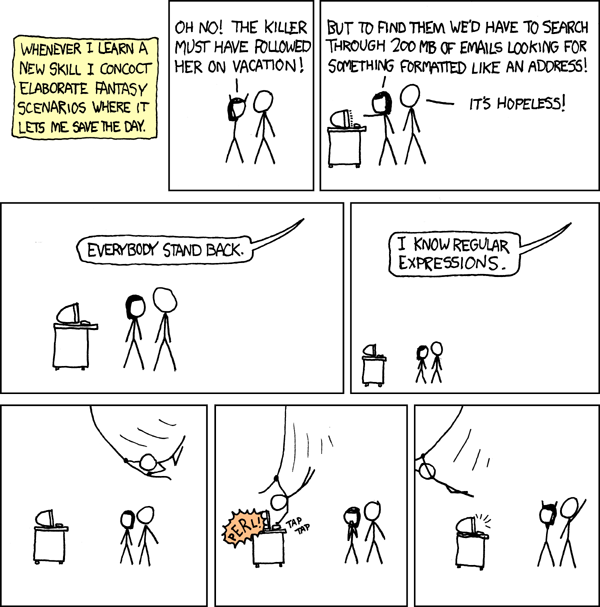
\includegraphics{img/xkcd_regular_expressions.png}
\caption{}
\end{figure}

(Bande dessinée de \href{http://xkcd.com}{Randall Munroe}.)


\chapter{Programmation Web : un cours condensé}

Vous lisez probablement ceci dans un navigateur web, donc vous êtes
susceptible d'être au moins un peu familier avec le World Wild Web. Ce
chapitre contient une rapide et superficielle introduction aux
différents éléments qui font fonctionner la toile, et la manière dont
ils sont liés au JavaScript. Les trois suivants sont plus pratiques et
présentent certaines des manières avec lesquelles JavaScript peut-être
utilisé pour inspecter et changer une page web.

\begin{center}\ding{67}\end{center}

L'Internet est fondamentalement un simple réseau d'ordinateurs couvrant
l'essentiel du monde. Les réseaux d'ordinateurs permettent aux
ordinateurs de s'envoyer des messages les uns aux autres. Les techniques
qui sont à la base de la mise en réseau sont un sujet intéressant mais
pas le propos de ce livre. Tout ce que vous avez à savoir est que,
généralement, un ordinateur, que nous appellerons serveur, attend que
d'autres ordinateurs se mettent à lui parler. Une fois qu'un autre
ordinateur, le client, ouvre une communication avec ce serveur, ils vont
échanger ce qui a besoin d'être échangé en utilisant un langage
spécifique, un protocole.

L'Internet est utilisé pour transporter des messages pour \emph{nombre}
de différents protocoles. Il y a des protocoles pour chatter, des
protocoles pour l'échange de fichiers, des protocoles utilisés par des
logiciels malicieux afin de contrôler l'ordinateur du pauvre schnock qui
l'a installé et ainsi de suite. Le protocole qui nous intéresse est
celui qu'on utilise pour le World Wide Web. Il s'appelle HTTP, ce qui
signifie Hyper Text Transfer Protocol (Protocole de Transfert Hyper
Texte) et il sert à retrouver des pages web et les fichiers qui leur
sont associés.

En communication HTTP, le serveur est l'ordinateur sur lequel la page
web est conservée. Le client est un ordinateur, comme le vôtre, qui
demande une page au serveur, afin de pouvoir l'afficher. Demander une
page ainsi s'appelle une «~requête HTTP~».

\begin{center}\ding{67}\end{center}

Les pages web et autres fichiers qui sont accessibles à travers
l'Internet sont identifiés par des «~URL~», ce qui est une abréviation
pour Universal Resource Locators (Localisateurs de Ressource Universel).
Une URL ressemble à ceci:

\begin{lstlisting}
http://acc6.its.brooklyn.cuny.edu/~phalsall/texts/taote-v3.html
\end{lstlisting}
Elle est composée de trois parties. Le début, \texttt{http://}, indique
que cette URL utilise le protocole HTTP. Il y a d'autres protocoles,
comme le FTP (File Transfer Protocol ou Protocole de Transfert de
Fichiers), qui utilisent eux aussi des URL. La partie suivante,
\texttt{acc6.its.brooklyn.cuny.edu}, nomme le serveur sur lequel cette
page peut-être trouvée. La fin de l'URL, \texttt{/\ensuremath{\sim}},
nomme le fichier spécifique sur ce serveur.

La plupart du temps, le World Wide Web est accessible grâce à un
navigateur. Après avoir tapé une URL ou cliqué un lien, le navigateur
fait la requête HTTP appropriée au serveur adéquat. Si tout se passe
bien, le serveur répond en renvoyant un ficher au navigateur, qui le
montre à l'utilisateur d'une façon ou d'une autre.

Quand, comme dans l'exemple, le fichier retrouvé est un document HTML,
il sera affiché comme une page web. Nous avons brièvement discuté d'HTML
dans le \href{chapter6.html}{chapitre 6}, où nous avons vu qu'il pouvait
référencer des fichiers image. Dans le \href{chapter9.html}{chapitre 9},
nous avons trouvé que les pages HTML peuvent contenir la balise
\texttt{\textless{}script\textgreater{}} pour charger des fichiers de
code JavaScript. Quand un document HTML s'affiche, un navigateur
récupére tous ces fichiers supplémentaires depuis leur serveur, de
manière à les ajouter au document.

\begin{center}\ding{67}\end{center}

Bien qu'une URL soit supposée pointer sur un fichier, il est possible
qu'un serveur web fasse quelque chose de plus compliqué que simplement
rechercher un ficher et l'envoyer au client. -- Il peut traiter ce
fichier d'une certaine manière en premier, ou peut-être n'y a-t-il pas
du tout de fichier, mais seulement un programme qui, quand on lui donne
une URL, a une façon de générer le document pertinent pour elle.

Des programmes qui transforment ou génèrent des documents sur un serveur
sont une façon populaire de rendre les pages web moins statiques. Quand
un fichier est juste un fichier, il est toujours le même, mais quand il
y a un programme pour le fabriquer chaque fois qu'il est demandé, il
peut être fait pour sembler différent à chaque utilisateur, en fonction
de son identification et de sss préférences. Cela peut aussi rendre la
gestion de contenu sur les pages web bien plus simple -- au lieu
d'ajouter un nouveau fichier HTML chaque fois que quelque chose de
nouveau est placé sur un site web, un nouveau document est stocké dans
un entrepôt central et le programme sait où le trouver et comment le
montrer aux clients.

Ce type de programmation web s'appelle programmation côté serveur. Cela
affecte le document avant qu'il ne soit envoyé à l'utilisateur. Dans
certains cas, il est pratique d'avoir un programme qui tourne
\emph{après} que la page a été envoyée, quand l'utilisateur la regarde.
Ceci s'appelle programmation côté client, car le programme tourne sur
l'ordinateur du client. La programmation web côté client est ce pour
quoi JavaScript a été inventé.

\begin{center}\ding{67}\end{center}

Faire tourner des programmes côté client comporte un problème implicite.
Vous ne pouvez jamais vraiment savoir à l'avance quels genres de
programmes la page que vous visitez va faire fonctionner. Si elle peut
envoyer des informations de votre ordinateur vers d'autres, endommager
quelque chose ou infiltrer votre système, surfer sur la toile pourrait
être une activité bien hasardeuse.

Pour résoudre ce dilemme, les navigateurs limitent sévèrement les choses
qu'un programme JavaScript peut faire. Il n'est pas permis de consulter
vos fichiers ou de modifier quoi que ce soit d'étranger à la page web
dont il provient. Isoler un environnement de programmation comme cela,
se nomme sand-boxing (jouer dans le bac à sable). Offrir aux programmes
suffisamment de place pour être utiles et en même temps les restreindre
suffisamment pour les empêcher de faire du mal, n'est pas une chose
simple à faire. Tous les quelques mois, un programmeur JavaScript
découvre une nouvelle façon de contourner les limitations, de faire
quelque chose de mal ou de transgresser les barrières qui entourent la
vie privée. Les responsables des navigateurs répondent en modifiant
leurs programmes pour rendre cette astuce impossible et tout va bien à
nouveau -- jusqu'à ce que le prochain problème soit découvert.

\begin{center}\ding{67}\end{center}

Une des premières astuces de JavaScript qui devint largement utilisée
est la méthode \texttt{open} de l'objet \texttt{window}. Elle prend une
URL comme argument et ouvrira une nouvelle fenêtre affichant cette URL.

\begin{lstlisting}
var perry = window.open("http://www.pbfcomics.com");
\end{lstlisting}
A moins que vous n'ayez désactivé le bloqueur de pop-up dans le
\href{chapter6.html}{chapitre 6}, il y a une chance que cette nouvelle
fenêtre soit bloquée. Il y a une bonne raison pour que les bloqueurs de
pop-up existent. Les programmeurs web, particulièrement ceux qui
essayent d'attirer l'attention des gens sur les publicités, ont
tellement abusé de cette pauvre méthode \texttt{window.open} qu'à
présent, la plupart des utilisateurs la détestent avec passion. Elle a
son utilité pourtant et dans ce livre nous l'utiliserons pour afficher
certains exemples de page. D'une manière générale, vos scripts ne
devraient pas ouvrir de nouvelle fenêtre sauf quand l'utilisateur le
demande.

Notez que, cp \texttt{open} (tout comme \texttt{setTimeout} et
compagnie) est une méthode de l'objet \texttt{window}, la partie
\texttt{window.} peut être enlevée. Quand une fonction est appelée «
normalement~», elle est appelée comme une méthode sur l'objet de plus
haut niveau, ce qu'est \texttt{window}. Personnellement, je pense que
\texttt{open} semble un peu générique, donc généralement je tape
\texttt{window.open}, qui indique clairement que c'est une fenêtre qui
est en cours d'ouverture.

La valeur retournée par \texttt{window.open} est une nouvelle fenêtre.
C'est l'objet global pour le script tournant dans cette fenêtre, et il
contient toutes les choses standards comme le constructeur
\texttt{Object} et l'objet \texttt{Math}. Mais si vous essayez d'y jeter
un oeil, la plupart des navigateurs ne vont (probablement) pas vous
laisser faire\ldots{}

\begin{lstlisting}
show(perry.Math);
\end{lstlisting}
C'est la partie du sand-boxing que j'ai mentionnée plus tôt. Les pages
ouvertes par votre navigateur peuvent afficher des informations qui vous
sont seulement destinées, par exemple sur des sites où vous vous êtes
identifiés, et il serait donc mauvais que n'importe quel script au
hasard puisse y aller et les lire. L'exception à cette règle, ce sont
les pages ouvertes pour le même domaine : quand un script tournant sur
une page de \texttt{eloquentjavascript.net} ouvre une autre page de ce
même domaine, il peut faire tout ce qu'il veut sur cette page.

Une fenêtre ouverte peut être fermée avec sa méthode \texttt{close}. Si
vous ne l'avez pas déjà fermée vous même\ldots{}

\begin{lstlisting}
perry.close();
\end{lstlisting}
D'autres types de sous-documents, comme les frames (documents dans un
document) sont aussi des fenêtres du point de vue d'un programme
JavaScript et ont leur propre environnement JavaScript. En fait,
l'environnement auquel vous avez accédé dans la console appartient à une
petite frame invisible quelque part dans cette page -- de cette manière,
il est un petit peu plus difficile pour vous d'accidentellement mettre
la pagaille dans toute la page.

\begin{center}\ding{67}\end{center}

Chaque objet fenêtre a une propriété \texttt{document}, qui contient un
objet représentant le document affiché dans la fenêtre. Cet objet
contient, par exemple, une propriété \texttt{location}, avec des
informations sur l'URL du document.

\begin{lstlisting}
show(document.location.href);
\end{lstlisting}
Mettre \texttt{document.location.href} à une nouvelle URL peut être
utilisé pour demander au navigateur de charger un autre document. Une
autre application de l'objet \texttt{document} est sa méthode
\texttt{write}. Cette méthode, quand on lui donne un argument texte,
écrit du HTML dans le document. Quand c'est utilisé dans un document
totalement chargé, cela remplacera le document complet par le HTML
donné, ce qui n'est généralement pas ce que vous voulez. L'idée est
d'avoir un script l'appelant pendant que le document est en cours de
chargement, dans ce cas le HTML écrit sera inséré dans le document à
l'endroit où la balise \texttt{script} l'a déclenché. C'est une manière
simple d'ajouter des éléments dynamiques à une page. Par exemple, voici
un document carrément simple affichant l'heure courante.

\begin{lstlisting}
print(horlogeParlante);
var temps = viewHTML(horlogeParlante);
\end{lstlisting}
\begin{lstlisting}
temps.close();
\end{lstlisting}
Souvent, la technique affichée dans le \href{chapter12.html}{chapitre
12} fournit une manière plus propre et plus souple de modifier un
document, mais occasionnellement, \texttt{document.write} est la manière
la plus belle et la plus simple de le faire.

\begin{center}\ding{67}\end{center}

Une autre application populaire du JavaScript dans les pages web tourne
autour des formulaires. Dans les cas où vous ne seriez pas tout à fait
sûr du rôle des «~formulaires~», laissez moi vous présenter un résumé
rapide.

Une requête HTTP élémentaire est une simple requête pour un fichier.
Quand ce fichier n'est pas vraiment un fichier passif, mais un programme
côté serveur, il peut devenir utile d'inclure des informations autres
qu'un nom de fichier dans la requête. Pour cela, les requêtes HTTP sont
autorisées à contenir des «~paramètres~» additionnels. Voici un exemple:

\begin{lstlisting}
http://www.google.com/search?q=empire%20aztec
\end{lstlisting}
Après le fichier (\texttt{/search}), l'URL continue avec un point
d'interrogation, suivi de paramètres. Cette requête a un paramètre,
nommé \texttt{q} (vraisemblablement pour `query', c'est à dire requête),
dont la valeur est \texttt{empire aztec}. La partie \texttt{\%20}
correspond à un espace. Il y a nombre de caractères qui peuvent
apparaître dans ces valeurs, comme les espaces, les esperluettes ou les
points d'interrogation. Ceux-ci sont remplacés par un \texttt{\%} suivi
par une valeur numérique \footnote{La valeur qu'un caractère prend est décidée par le standard ASCII, qui assigne les nombres 0 à 127 à un ensemble de lettres et symboles utilisés par l'alphabet Latin. Ce standard est un précurseur du standard Unicode mentionné dans le \href{chapter2.html}{chapitre 2}.}, ce qui a la même
fonction que les antislash utilisés dans les textes et expressions
régulières, mais est encore plus illisible.

JavaScript fournit les fonctions \texttt{encodeURIComponent} et
\texttt{decodeURIComponent} pour ajouter ces codes aux textes et
également les enlever.

\begin{lstlisting}
var encode = encodeURIComponent("empire aztec");
show(encode);
show(decodeURIComponent(encode));
\end{lstlisting}
Quand une requête contient plus d'un paramètre, ils sont séparés par une
esperluette, comme dans\ldots{}

\begin{lstlisting}
http://www.google.com/search?q=empire%20aztec&lang=fr
\end{lstlisting}
\begin{center}\ding{67}\end{center}

Un formulaire, essentiellement, est une manière de rendre facile aux
utilisateurs des navigateurs la création de ces URL paramétrées. Il
contient un nombre de champs, comme des boîtes d'entrée de texte, des
cases à cocher qui peuvent être «~cochées~» et «~décochées~» ou des
bidules permettant de choisir parmi un ensemble de valeurs. Il contient
en général aussi un bouton de «~soumission~» et, invisible à
l'utilisateur, une URL «~action~» à laquelle il sera envoyé. Quand on
clique sur le bouton «~soumettre~» ou qu'on appuie sur la touche Entrée,
les informations qui ont été saisies dans les champs sont ajoutées comme
paramètres à cette URL action, et le navigateur va demander cette URL.

Voici le HTML pour un formulaire simple :

\begin{lstlisting}
<form name="info_utilisateur" method="get" action="info.html">
  <p>S'il vous plaît donnez-nous vos informations, afin que nous puissions vous envoyer du spam.</p>
  <p>Nom: <input type="text" name="nom"/></p>
  <p>E-Mail: <input type="text" name="email"/></p>
  <p>Sexe: <select name="sexe">
            <option>Homme</option>
            <option>Femme</option>
            <option>Autre</option>
          </select></p>
  <p><input name="envoyer" type="submit" value="Envoyer !"/></p>
</form>
\end{lstlisting}
Le nom du formulaire peut être utilisé pour y accéder avec JavaScript,
comme nous allons le voir dans un moment. Les noms des champs
déterminent les noms des paramètres HTTP qui sont utilisés afin de
stocker leurs valeurs. Envoyer ce formulaire peut produire une URL comme
ceci:

\begin{lstlisting}
http://planetspam.com/info.html?nom=Ted&email=ted@zork.com&sexe=Homme
\end{lstlisting}
Il y a nombre d'autres tags et propriétés qui peuvent être utilisés dans
les formulaires mais dans ce livre nous nous en tiendrons aux plus
simples, afin de nous concentrer sur JavaScript.

\begin{center}\ding{67}\end{center}

La propriété \texttt{method="get"} du formulaire d'exemple ci-dessus
indique que ce formulaire doit encoder les valeurs qu'on lui donne en
tant que paramètres d'URL, comme montré avant. Il existe une méthode
alternative pour envoyer les paramètres, qui s'appelle \texttt{post}.
Une requête HTTP utilisant la méthode \texttt{post} contient, en plus
d'une URL, un bloc de données. Un formulaire utilisant la méthode
\texttt{post} met les valeurs de ses paramètres dans ce bloc de données
plutôt que dans l'URL.

Quand on envoie de grandes quantités de données, la méthode \texttt{get}
va générer des URL d'un kilomètre de long, donc \texttt{post} est
généralement plus pratique. Mais la différence entre les deux méthodes
n'est pas juste une question de convenance. Traditionnellement, les
requêtes \texttt{get} sont utilisées pour demander un document au
serveur, alors que les requêtes \texttt{post} sont utilisées pour
déclencher une action qui change quelque chose sur le serveur. Par
exemple, obtenir une liste des messages récents d'un forum Internet
serait une requête \texttt{get}, alors qu'ajouter un nouveau message
serait une requête \texttt{post}. Il y a une bonne raison pour laquelle
la plupart des pages suivent cette distinction -- les programmes qui
explorent automatiquement le web, comme ceux utilisés par les moteurs de
recherche, vont généralement seulement faire des requêtes \texttt{get}.
Si des changements sur un site peuvent être faits par une requête
\texttt{get}, ces robots d'exploration bien intentionnés pourraient
faire pas mal de dégâts.

\begin{center}\ding{67}\end{center}

Quand le navigateur affiche une page contenant un formulaire, les
programmes JavaScript peuvent inspecter et modifier les valeurs qui sont
entrées dans les champs du formulaire. Cela ouvre des possibilités pour
toutes sortes d'astuces, comme vérifier les valeurs avant qu'elles ne
soient envoyées au serveur ou remplir automatiquement certains champs.

Le formulaire affiché ci-dessus peut être trouvé dans le fichier
\texttt{example\_getinfo.html}. Ouvrez-le.

\begin{lstlisting}
var formulaire = window.open("example_getinfo.html");
\end{lstlisting}
Quand une URL ne contient pas un nom de serveur, elle est appelée URL
relative. Les URL relatives sont interprétées par le navigateur pour
référencer des fichiers sur le même serveur que le document en cours. A
moins qu'il ne commence avec un slash, le chemin (ou répertoire) du
document en cours est aussi conservé et le chemin donné lui est ajouté.

Nous ajouterons une vérification de validité au formulaire, afin qu'il
soumette seulement si le champ nom n'est pas laissé vide et si le champ
e-mail contient quelque chose qui ressemble à une addresse e-mail
valide. Parce que nous ne voulons plus que le formulaire soit soumis
immédiatement quand le bouton «~Envoyer !~» est cliqué. Sa propriété
\texttt{type} a été changée de \texttt{"submit"} à \texttt{"button"}, ce
qui le change en un bouton ordinaire sans aucun effet. -- Le
\href{chapter13.html}{chapitre 13} montrera une \emph{bien} meilleure
manière de faire ceci, mais pour l'instant, nous utilisons la méthode
naïve.

\begin{center}\ding{67}\end{center}

Afin de travailler avec la fenêtre nouvellement ouverte (si vous l'avez
fermée, rouvrez-la d'abord), nous lui «~attachons~» la console, comme
ceci:

\begin{lstlisting}
attach(formulaire);
\end{lstlisting}
Après avoir fait ceci, le code lancé de la console tournera dans la
fenêtre donnée. Pour vérifier que nous fonctionnons effectivement avec
la bonne fenêtre, nous pouvons regarder les propriétés \texttt{location}
et \texttt{title} du document.

\begin{lstlisting}
print(document.location.href);
print(document.title);
\end{lstlisting}
Étant donné que nous avons entré un nouvel environnement, les variables
précédemment définies, comme \texttt{formulaire}, ne sont plus
présentes.

\begin{lstlisting}
show(formulaire);
\end{lstlisting}
Pour revenir à notre environnement de départ, nous pouvons utiliser la
fonction \texttt{detach} (sans argument). Mais d'abord, nous avons à
ajouter le système de validation au formulaire.

\begin{center}\ding{67}\end{center}

Toute balise HTML affichée dans un document a un objet JavaScript
associé. Ces objets peuvent être utilisés pour inspecter et manipuler
presque tout aspect du document. Dans ce chapitre, nous allons
travailler avec les objets pour formulaires et champs de formulaire. Le
\href{chapter12.html}{chapitre 12} traite de façon plus détaillée de ces
objets.

L'objet \texttt{document} a une propriété nommée \texttt{forms}, qui
contient des liens vers tous les formulaires du document, par nom. Notre
formulaire a une propriété \texttt{name="info\_utilisateur"}, afin
d'être trouvable sous la propriété \texttt{info\_utilisateur}.

\begin{lstlisting}
var formulaireUtilisateur = document.forms.info_utilisateur;
print(formulaireUtilisateur.method);
print(formulaireUtilisateur.action);
\end{lstlisting}
Dans ce cas, les propriétés \texttt{method} et \texttt{action} qui ont
été données à la balise HTML \texttt{form} sont aussi présentes comme
propriétés de l'objet JavaScript. C'est souvent le cas, mais pas
toujours: Certaines propriétés HTML sont orthographiées différemment en
JavaScript, d'autres ne sont pas présentes du tout. Le
\href{chapter12.html}{chapitre 12} exposera un moyen d'obtenir toutes
les propriétés.

L'objet de la balise \texttt{form} a une propriété \texttt{elements},
qui se réfère a un objet contenant les champs du formulaire, par nom.

\begin{lstlisting}
var champsNom = formulaireUtilisateur.elements.nom;
champsNom.value = "Eugène";
\end{lstlisting}
Les objets d'entrée texte ont une propriété \texttt{value}, qui peut
être utilisée pour lire et changer leur contenu. Si vous regardez la
fenêtre du formulaire après le fonctionnement du code ci-dessus, vous
verrez que le nom a été rempli.

\begin{center}\ding{67}\end{center}

Ex. 11.1

Être capable de lire les valeurs des champs du formulaire rend possible
l'écriture d'une fonction \texttt{valideInfo}, qui prend un objet
formulaire comme argument et retourne une valeur booléenne:
\texttt{true} quand le champ \texttt{nom} n'est pas vide et le champ
\texttt{email} contient quelque chose qui ressemble à une adresse email,
sinon \texttt{false}. Ecrivez cette fonction.

\begin{lstlisting}
function valideInfo(formulaire) {
  return formulaire.elements.nom.value != "" &&
    /^.+@.+\.\w{2,3}$/.test(formulaire.elements.email.value);
}

show(valideInfo(document.forms.info_utilisateur));
\end{lstlisting}
Vous avez bien pensé à utiliser une expression régulière pour la
vérification de l'e-mail, n'est-ce pas ?

\begin{center}\ding{67}\end{center}

Tout ce que nous avons à faire maintenant est de déterminer ce qui
arrive quand les gens cliquent sur le bouton «~Envoyer !~». Pour
l'instant, il ne se passe rien du tout. Cela sera corrigé en réglant sa
propriété \texttt{onclick}.

\begin{lstlisting}
formulaireUtilisateur.elements.envoyer.onclick = function() {
  alert("Clique.");
};
\end{lstlisting}
Tout comme les actions données à \texttt{setInterval} et
\texttt{setTimeout} (\href{chapter8.html}{chapitre 8}), la valeur
stockée dans une propriété \texttt{onclick} (ou similaire) peut être
soit une fonction soit une chaîne de code JavaScript. Dans ce cas, nous
lui donnons une fonction qui ouvre une fenêtre d'alerte. Essayez de la
sélectionner.

\begin{center}\ding{67}\end{center}

Ex. 11.2

Finissez le validateur de formulaire en donnant à la propriété
\texttt{onclick} du bouton une nouvelle valeur -- une fonction qui
vérifie le formulaire, le soumet quand il est valide, ou génère un
message d'avertissement quand il ne l'est pas. Il est utile de savoir
que les objets formulaires ont une méthode \texttt{submit} qui ne prend
aucun paramètre et soumet le formulaire.

\begin{lstlisting}
formulaireUtilisateur.elements.envoyer.onclick = function() {
  if (valideInfo(formulaireUtilisateur))
    formulaireUtilisateur.submit();
  else
    alert("Donnez-nous un nom et une adresse e-mail valides !");
};
\end{lstlisting}
\begin{center}\ding{67}\end{center}

Une autre astuce liée aux entrées de formulaire, ainsi que d'autres
choses qui peuvent être «~sélectionnées~», comme les boutons ou liens,
est la méthode \texttt{focus}. Quand vous savez avec certitude qu'un
utilisateur voudra saisir dans un certain champ dès qu'il entre dans la
page, vous pouvez faire en sorte que votre script y place le curseur,
afin qu'il n'ait pas à cliquer pour le sélectionner d'une quelconque
manière.

\begin{lstlisting}
formulaireUtilisateur.elements.nom.focus();
\end{lstlisting}
Puisque le formulaire est dans une autre fenêtre, il n'est pas forcément
évident que quelque chose ait été sélectionné, cela dépend du navigateur
que vous utilisez. Certaines pages vont aussi automatiquement faire
passer le curseur sur le champ suivant quand il semble que vous ayez
fini de remplir un champ -- par exemple, quand vous tapez un code postal.
Ceci ne devrait pas être fait de manière exagérée -- cela donne à la page
un comportement auquel l'utilisateur ne s'attend pas. S'il est habitué à
la tabulation pour déplacer le curseur manuellement ou a fait une erreur
sur le dernier caractère et veut l'enlever, ce curseur sauteur magique
est très ennuyeux.

\begin{center}\ding{67}\end{center}

\begin{lstlisting}
detach();
\end{lstlisting}
Testez le validateur. Quand vous entrez une information valide et
cliquez sur le bouton, le formulaire devrait se soumettre. Si la console
y est toujours attachée, cela la fera se détacher, car la page se
rechargera et l'environnement JavaScript sera remplacé par un nouveau.

Si vous n'avez pas encore clos la fenêtre de formulaire, ceci la
fermera.

\begin{lstlisting}
formulaire.close();
\end{lstlisting}
\begin{center}\ding{67}\end{center}

Cela peut sembler simple, mais je vous assure que la programmation côté
client n'est pas de tout repos. Cela peut même parfois être une épreuve
douloureuse. Pourquoi ? Parce que les programmes qui sont supposés
tourner sur l'ordinateur client doivent généralement fonctionner dans
les navigateurs les plus populaires. Chacun de ces navigateurs a
tendance à fonctionner de manière légèrement différente. Pour rendre les
choses plus complexes, chacun d'entre eux contient son propre ensemble
de problèmes. Ne présumez pas qu'un programme est sans bug juste parce
qu'il a été fait par une entreprise qui pèse plusieurs milliards de
dollars. Donc il nous revient à nous, développeurs web, de
rigoureusement tester nos programmes, d'arriver à comprendre ce qui va
pas et de trouver des manières de contourner les problèmes.

Certains d'entre vous peuvent penser «~Je vais juste remonter tous les
problèmes/bugs que je trouve aux fabricants du navigateur et ils vont
certainement les résoudre immédiatement~». Ces gens se préparent à une
grosse déception. Les plus récentes versions d'Internet Explorer, le
navigateur qui est toujours utilisé par quelque soixante dix pour cent
des surfeurs de la toile (et que chaque développeur web aime à taquiner)
contient toujours des bugs qui sont connus depuis plus de cinq ans. De
sérieux bugs en plus.

Mais que cela ne vous décourage pas. Avec un état d'esprit du genre
obsessionnel-compulsif comme il convient, de tels problèmes lancent des
défis merveilleux. Et pour ceux d'entre vous qui n'aiment pas perdre
leur temps, être prudent et éviter les recoins obscurs des
fonctionnalités du navigateur vous évitera de tomber sur des problèmes
trop embarrassants.

\begin{center}\ding{67}\end{center}

A part les bugs, les différences de conception d'interface entre
navigateurs produisent un défi intéressant. La situation en cours
ressemble à quelque chose comme ceci : d'un côté, il y a tous les «
petits~» navigateurs : Firefox, Safari et Opéra sont les plus importants
mais il en existe d'autres. Ces navigateurs font tous un effort
raisonnable pour adhérer à un ensemble de standards qui ont été
développés ou sont en train d'être développés, par le W3C, une
organisation qui essaie de faire de la toile un environnement moins
désordonné en définissant des interfaces standards pour des choses comme
ceci. D'un autre côté, il y a Internet Explorer, le navigateur de
Microsoft, qui a grandi jusqu'à dominer à une époque quand la plupart de
ces standards n'existaient pas vraiment encore et n'a guère fait
d'efforts pour s'ajuster à ce que les autres font.

Dans certains domaines, tels que la façon dont le contenu d'un document
HTML peut être interprété par le JavaScript
(\href{chapter12.html}{chapitre 12}), les standards sont basés sur la
méthode inventée par Internet Explorer et les choses marchent plus ou
moins de la même façon pour tous les navigateurs. Dans d'autres
domaines, tels que la façon dont les événements sont gérés (clic de
souris, touche du clavier enfoncée et autres), Internet Explorer
fonctionne différemment des autres.

Pendant longtemps, en partie à cause du manque de jugeotte du
développeur JavaScript moyen, en partie à cause des incompatibilités
entre navigateurs qui étaient bien pires quand les navigateurs comme
Internet Explorer versions 4 et 5 et les vieilles versions de Netscape
étaient encore fréquentes, la manière habituelle de gérer de telles
différences était de détecter quel navigateur l'utilisateur faisait
tourner et de disperser dans le code des solutions alternatives pour
chaque navigateur -- si c'est Internet Explorer, fais ceci, si c'est
Netscape, fais cela, et si c'est n'importe quel autre navigateur auquel
nous n'avons pas pensé, garde l'espoir que tout se passera pour le
mieux. Vous pouvez imaginer à quel point ces programmes étaient hideux,
obscurs et longs.

Nombre de sites pouvaient aussi refuser de se charger quand ils étaient
ouverts dans un navigateur qui n'était «~pas supporté~». Cela obligea
quelques-uns des navigateurs mineurs à ravaler leur fierté et prétendre
qu'ils étaient Internet Explorer, juste assez pour être autorisés à
charger de telles pages. Les propriétés de l'objet \texttt{navigator}
contiennent des informations sur le navigateur dans lequel une page a
été chargée, mais à cause de ces mensonges cette information n'est pas
particulièrement fiable. Voyez ce que dit le vôtre\footnote{Certains navigateurs semblent cacher les propriétés de l'objet \texttt{navigator}, dans ce cas ce qui suit n'affichera rien.} :

\begin{lstlisting}
forEachIn(navigator, function(nom, valeur) {
  print(nom, " = ", valeur);
});
\end{lstlisting}
Une meilleur approche consiste à essayer «~d'isoler~» nos programmes des
différences entre navigateurs. Si vous devez, par exemple, en découvrir
plus sur un événement, comme le clic que nous avons géré en modifiant la
propriété \texttt{onclick} de notre bouton d'envoi, vous devez regarder
l'objet de haut niveau nommé \texttt{event} dans Internet Explorer, mais
vous devez utiliser le premier argument passé à la fonction gérant cet
évènement dans les autres navigateurs. Pour gérer ceci, et nombre
d'autres différences liées aux évènements, on peut écrire une fonction
d'aide pour attacher les évènements aux choses, elle prendra soin de
toute la plomberie et permettra aux fonctions de gestion d'événements
d'être les mêmes pour tous les navigateurs. Dans le
\href{chapter13.html}{chapitre 13} nous écrirons une fonction de ce
genre.

(Note: Les caprices de navigateur mentionnés dans les chapitres suivants
font référence à l'état en cours en début 2007, et peuvent ne plus être
aussi précis sur certains points.)

\begin{center}\ding{67}\end{center}

Ces chapitres ne donneront qu'une introduction superficielle du sujet
des interfaces des navigateurs. Elles ne sont le principal sujet de ce
livre et elles sont suffisamment complexes pour remplir un livre par
elles-mêmes. Quand vous aurez compris les bases de ces interfaces (et
compris quelque chose à propos d'HTML), ce ne sera pas trop difficile de
rechercher des informations spécifiques en ligne. Les documentations des
interfaces des navigateurs
\href{http://www.mozilla.org/docs/dom/domref/dom\_shortTOC.html}{Firefox}
et \href{http://msdn2.microsoft.com/library/yek4tbz0p.aspx}{Internet
Explorer} constituent de bons points de départ.

Les informations dans les prochains chapitres n'aborderont pas les
caprices des navigateurs de «~génération antérieure~». Elles parlent
d'Internet Explorer 6, Firefox 1.5, Opera 9, Safari 3, ou n'importe
quelle version plus récente de ces mêmes navigateurs. La plus grande
part sera aussi applicable aux modernes mais obscurs navigateurs comme
Konqueror, mais cela n'a pas été complètement vérifié. Heureusement, ces
navigateurs de génération antérieure ont plus ou moins disparu, et ne
sont plus guère utilisés.

Il y a, malgré tout, un groupe d'utiliseurs web qui vont toujours
utiliser un navigateur sans JavaScript. Une large part de ce groupe est
constitué de personnes utilisant un navigateur graphique usuel, mais
avec JavaScript désactivé pour des raisons de sécurité. Ensuite ceux qui
utilisent des navigateurs textes, ou navigateurs pour personnes
aveugles. Quand on travaille sur un site «~sérieux~», c'est une bonne
idée de commencer avec un simple système HTML qui fonctionne et ensuite
d'ajouter des bidouilles non essentielles et des trucs pratiques avec
JavaScript.


\chapter{Le modèle d'objet-document}

Dans le \href{chapter11.html}{chapitre 11} nous avons vu les objets
JavaScript qui font référence aux balises \texttt{form} et
\texttt{input} du document HTML. De tels objets font partie d'une
structure appelée le modèle d'objet-document (DOM). Chaque élément du
document est représenté dans ce modèle, on peut l'examiner et interagir
avec lui.

Les documents HTML ont ce qu'on peut appeler une structure hiérarchique.
Chaque élément (ou balise) à l'exception de la balise de premier niveau
\texttt{\textless{}html\textgreater{}} est contenu dans un autre
élément, son parent. Cet élément peut en retour contenir d'autres
éléments. Vous pouvez vous le représenter comme une sorte d'arbre
généalogique.

\begin{figure}[ht!]
\centering
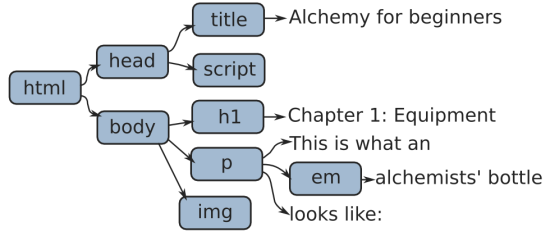
\includegraphics{img/html.png}
\caption{}
\end{figure}

Le modèle document-objet est basé sur une telle vue du document.
Veuillez noter que l'arbre contient deux types d'éléments : les nœuds,
représentés comme des boîtes bleues et de simples morceaux de texte. Les
morceaux de texte sont comme nous le verrons assez différents des autres
éléments. L'une de ces différences est qu'ils n'ont jamais d'enfants.

Ouvrez le fichier \texttt{example\_alchemy.html} qui contient le
document présenté dans l'image et attachez-y la console.

\begin{lstlisting}
attach(window.open("example_alchemy.html"));
\end{lstlisting}
L'objet de la racine de l'arbre document, le nœud \texttt{html},
peut-être atteint via la propriété \texttt{documentElement} de l'objet
\texttt{document}. La plupart du temps, nous avons plutôt besoin de la
partie \texttt{body} du document qui se trouve à \texttt{document.body}.

\begin{center}\ding{67}\end{center}

Les liens entre ces nœuds sont disponibles sous forme de propriétés de
l'objet nœud. Chaque objet DOM possède une propriété \texttt{parentNode}
qui fait référence à l'objet dans lequel il est contenu, si objet il y
a. Ces parents ont aussi des liens pointant vers leurs enfants. Mais
parce qu'il peut y avoir plusieurs enfants, ils sont stockés dans un
pseudo-tableau appelé \texttt{childNodes}.

\begin{lstlisting}
show(document.body);
show(document.body.parentNode);
show(document.body.childNodes.length);
\end{lstlisting}
Par commodité, il y a aussi des liens appelés \texttt{firstChild} et
\texttt{lastChild}, pointant respectivement au premier et au dernier
enfant à l'intérieur d'un nœud ou \texttt{null} quand il n'y a pas
d'enfant.

\begin{lstlisting}
show(document.documentElement.firstChild);
show(document.documentElement.lastChild);
\end{lstlisting}
Enfin, il y a des propriétés nommées \texttt{nextSibling} et
\texttt{previousSibling}, qui pointent vers les nœuds présents aux côtés
d'un autre nœud -- les nœuds qui sont des enfants du même parent, venant
avant ou après le nœud courant. Encore une fois, lorsque ces nœuds ne
sont pas présents, la valeur de ces propriétés est \texttt{null}.

\begin{lstlisting}
show(document.body.previousSibling);
show(document.body.nextSibling);
\end{lstlisting}
\begin{center}\ding{67}\end{center}

Pour savoir si un nœud représente un simple morceau de texte ou un nœud
HTML, nous pouvons jeter un œil à sa propriété \texttt{nodeType}. Elle
contiendra un nombre, \texttt{1} pour un nœud classique et \texttt{3}
pour un nœud texte. Il existe en fait d'autres sortes d'objets qui
possèdent un \texttt{nodeType}, comme l'objet \texttt{document} qui
vaudra \texttt{9}, mais l'usage le plus commun de cette propriété est la
distinction entre les nœuds textes et les autres nœuds.

\begin{lstlisting}
function isTextNode(noeud) {
  return noeud.nodeType == 3;
}

show(isTextNode(document.body));
show(isTextNode(document.body.firstChild.firstChild));
\end{lstlisting}
Les nœuds classiques ont une propriété appelée \texttt{nodeName},
indiquant le type de balise HTML qu'ils représentent. En revanche, les
nœuds textes ont une propriété \texttt{nodeValue}, ayant pour valeur
leur contenu texte.

\begin{lstlisting}
show(document.body.firstChild.nodeName);
show(document.body.firstChild.firstChild.nodeValue);
\end{lstlisting}
Les propriétés \texttt{nodeName} sont toujours mises en majuscules,
c'est quelque chose qui doit être pris en compte si jamais vous voulez
les comparer à quoi que ce soit.

\begin{lstlisting}
function isImage(noeud) {
  return !isTextNode(noeud) && noeud.nodeName == "IMG";
}

show(isImage(document.body.lastChild));
\end{lstlisting}
\begin{center}\ding{67}\end{center}

Ex. 12.1

Écrivez une fonction \texttt{asHTML} qui, appelée avec un nœud DOM,
produira une chaîne représentant le texte HTML de ce nœud et de ses
éléments. Vous pouvez ignorer les attributs, afficher juste les nœuds
comme \texttt{\textless{}nodename\textgreater{}}. La fonction
\texttt{escapeHTML} du \href{chapter10.html}{chapitre 10} est disponible
afin d'échapper correctement le contenu des nœuds textes.

Indice : Récursion!

\begin{lstlisting}
function asHTML(noeud) {
  if (isTextNode(noeud))
    return escapeHTML(noeud.nodeValue);
  else if (noeud.childNodes.length == 0)
    return "<" + noeud.nodeName + "/>";
  else
    return "<" + noeud.nodeName + ">" +
           map(asHTML, noeud.childNodes).join("") +
           "</" + noeud.nodeName + ">";
}

print(asHTML(document.body));
\end{lstlisting}
\begin{center}\ding{67}\end{center}

En réalité, les nœuds ont déjà quelque chose de similaire à
\texttt{asHTML}. Leur propriété \texttt{innerHTML} peut être utilisée
afin de récupérer le texte HTML \emph{à l'intérieur} du nœud, sans les
balises du nœud en question. Quelques navigateurs Web, mais pas tous,
prennent aussi en charge la propriété \texttt{outerHTML}, qui inclut le
nœud lui-même.

\begin{lstlisting}
print(document.body.innerHTML);
\end{lstlisting}
Certaines de ces propriétés peuvent aussi être modifiées. Modifier le
\texttt{innerHTML} d'un nœud ou la \texttt{nodeValue} d'un nœud texte
changera son contenu. À noter que dans le premier cas, la chaîne donnée
est interprétée comme du HTML alors que dans le second cas elle est
interprétée comme du simple texte.

\begin{lstlisting}
document.body.firstChild.firstChild.nodeValue =
  "Chapitre 1 : La grande importance de la bouteille";
\end{lstlisting}
Ou\ldots{}

\begin{lstlisting}
document.body.firstChild.innerHTML =
  "Connaissiez-vous déjà la balise « blink » ? <blink>Oh joie !</blink>";
\end{lstlisting}
\begin{center}\ding{67}\end{center}

Nous avons accédé à des nœuds au travers d'une série de propriétés
\texttt{firstChild} et \texttt{lastChild}. Cela peut fonctionner, mais
c'est assez verbeux et facilement cassable -- si nous ajoutons un autre
nœud au début de notre document, \texttt{document.body.firstChild} ne
pointera plus sur l'élément \texttt{h1} et si le code prétend le
contraire il se trompe. En plus de cela, certains navigateurs Web
ajouteront des nœuds textes pour des choses comme les espaces et les
retours à la ligne entre les balises alors que d'autres non. La
représentation exacte de l'arbre DOM peut varier.

Comme alternative, il vous est possible de donner un attribut
\texttt{id} aux éléments auxquels vous avez besoin d'accéder. Dans la
page d'exemple, l'image à un id \texttt{"image"}, nous pouvons
l'utiliser pour retrouver l'image.

\begin{lstlisting}
var image = document.getElementById("image");
show(image.src);
image.src = "img/ostrich.png";
\end{lstlisting}
Quand vous tapez \texttt{getElementById}, notez que la dernière lettre
est en minuscule. Faites donc attention, lorsque vous le taperez
souvent, au syndrome du canal carpien. Parce que
\texttt{document.getElementById} est un nom ridiculement long pour une
opération aussi commune, l'abréger par \texttt{\$} est devenu une
convention au sein des développeurs JavaScript. \texttt{\$}, comme vous
vous en souvenez peut-être, est considéré comme une lettre par
JavaScript et c'est donc un nom de variable valide.

\begin{lstlisting}
function $(id) {
  return document.getElementById(id);
}
show($("image"));
\end{lstlisting}
Les nœuds DOM ont aussi une méthode \texttt{getElementsByTagName} (un
autre nom sympa et court), qui appelée avec un nom de balise, retourne
un tableau de tous les nœuds de ce type contenu dans le nœud sur lequel
la méthode a été appelée.

\begin{lstlisting}
show(document.body.getElementsByTagName("BLINK")[0]);
\end{lstlisting}
\begin{center}\ding{67}\end{center}

Une autre chose que nous pouvons faire avec ces nœuds est d'en créer de
nouveaux nous-même. Cela rend possible l'ajout d'éléments dans un
document, qui pourront être utilisés pour créer des effets intéressants.
Malheureusement l'interface permettant cela est extrêmement mal fichue.
Mais il est possible de remédier à cela avec des fonctions d'aide.

L'objet \texttt{document} possède les méthodes \texttt{createElement} et
\texttt{createTextNode}. La première est utilisée pour créer un nœud
classique, la seconde, comme son nom le suggère, pour créer un nœud
texte.

\begin{lstlisting}
var deuxiemeEntete = document.createElement("H1");
var deuxiemeChapitre = document.createTextNode("Chapitre 2 : Magie intense");
\end{lstlisting}
Nous voulons ensuite mettre le titre dans l'élément \texttt{h1}, puis
ajouter cet élément au document. Le moyen le plus simple de le faire est
la méthode \texttt{appendChild} qui peut-être appelée sur chaque nœud
qui n'est pas un nœud texte.

\begin{lstlisting}
deuxiemeEntete.appendChild(deuxiemeChapitre);
document.body.appendChild(deuxiemeEntete);
\end{lstlisting}
Souvent, vous voudrez aussi ajouter des attributs à ces nouveaux nœuds .
Par exemple, une balise \texttt{img} (image) est plutôt inutile sans la
propriété \texttt{src} qui dit au navigateur quelle image il doit
afficher. La plupart des attributs peuvent être retrouvés directement
comme des propriétés du nœud DOM mais il y a aussi les méthodes
\texttt{setAttribute} et \texttt{getAttribute}, qui sont utilisées pour
accéder aux attributs de façon plus générale :

\begin{lstlisting}
var nouvelleImage = document.createElement("IMG");
nouvelleImage.setAttribute("src", "img/Hiva Oa.png");
document.body.appendChild(nouvelleImage);
show(nouvelleImage.getAttribute("src"));
\end{lstlisting}
\begin{center}\ding{67}\end{center}

Mais, lorsque l'on veut créer davantage que quelques nœuds simples , il
devient assez assommant de créer chaque nœud avec un appel vers
\texttt{document.createElement} ou \texttt{document.createTextNode}, et
ensuite d'y ajouter les attributs et les éléments un par un.
Heureusement, il n'est pas trop difficile d'écrire une fonction qui
ferait le plus gros du travail pour nous. Avant de s'y mettre, il y a un
petit détail qu'il faut prendre en compte : la méthode
\texttt{setAttribute}, qui fonctionne correctement sur la plupart des
navigateurs, ne fonctionne pas toujours sur Internet Explorer. Les noms
de certains attributs HTML ont déjà un sens particulier en JavaScript,
de ce fait, la propriété de l'objet correspondant obtient un nom ajusté.
Plus spécifiquement, l'attribut \texttt{class} devient
\texttt{className}, \texttt{for} devient \texttt{htmlFor} et
\texttt{checked} est renommé en \texttt{defaultChecked}. Sur Internet
Explorer, \texttt{setAttribute} et \texttt{getAttribute} fonctionnent
aussi avec ces noms ajustés, à la place des noms HTML originaux ce qui
peut être source de confusion. En plus de cela l'attribut
\texttt{style}, qui sera abordé plus tard dans ce chapitre avec
\texttt{class}, ne peut être défini avec \texttt{setAttribute} sur ce
navigateur.

Une solution de contournement pourrait ressembler à quelque chose comme
ça :

\begin{lstlisting}
function setNodeAttribute(noeud, attribut, valeur) {
  if (attribut == "class")
    noeud.className = valeur;
  else if (attribut == "checked")
    noeud.defaultChecked = valeur;
  else if (attribut == "for")
    noeud.htmlFor = valeur;
  else if (attribut == "style")
    noeud.style.cssText = valeur;
  else
    noeud.setAttribute(attribut, valeur);
}
\end{lstlisting}
À chaque fois qu'Internet Explorer dévie du comportement des autres
navigateurs, il fait quelque chose qui fonctionne dans tous les cas. Ne
vous inquiétez pas des détails, c'est ce genre d'astuces sales dont nous
aimerions ne pas avoir besoin mais que les navigateurs non conformes
nous obligent à écrire. Considérant ceci, il est possible d'écrire une
simple fonction pour créer des éléments DOM.

\begin{lstlisting}
function dom(nom, attributs) {
  var noeud = document.createElement(nom);
  if (attributs) {
    forEachIn(attributs, function(nom, valeur) {
      setNodeAttribute(noeud, nom, valeur);
    });
  }
  for (var i = 2; i < arguments.length; i++) {
    var noeudEnfant = arguments[i];
    if (typeof noeudEnfant == "string")
      noeudEnfant = document.createTextNode(noeudEnfant);
    noeud.appendChild(noeudEnfant);
  }
  return noeud;
}

var nouveauParagraphe =
  dom("P", null, "Un paragraphe avec un ",
      dom("A", {href: "http://fr.wikipedia.org/wiki/Alchimie"},
          "lien"),
      " à l'intérieur.");
document.body.appendChild(nouveauParagraphe);
\end{lstlisting}
La fonction \texttt{dom} crée un arbre DOM. Son premier argument donne
le nom de la balise du nœud, son second argument est un objet contenant
l'attribut du nœud, ou \texttt{null} quand aucun attribut n'est requis.
Après quoi, n'importe quel nombre d'arguments peut suivre et ils seront
ajoutés au nœud comme enfants nœuds. Quand des chaînes apparaissent ici,
elles sont ajoutées dans un nœud texte.

\begin{center}\ding{67}\end{center}

\texttt{appendChild} n'est pas le seul moyen d'insérer des nœuds dans un
autre nœud. Quand le nouveau nœud ne doit pas apparaître à la fin de son
parent, la méthode \texttt{insertBefore} peut-être utilisée pour le
placer avant un autre nœud enfant. Elle prend le nouveau nœud comme
premier argument et l'élément existant comme second argument.

\begin{lstlisting}
var lien = nouveauParagraphe.childNodes[1];
nouveauParagraphe.insertBefore(dom("STRONG", null, "super "), lien);
\end{lstlisting}
Si un nœud possèdant déjà un \texttt{parentNode} est placé ailleurs, il
est automatiquement supprimé de sa position actuelle -- les nœuds ne
peuvent pas exister dans le document à plus d'un endroit à la fois.

Quand un nœud doit être remplacé par un autre, utilisez la méthode
\texttt{replaceChild}, qui prend encore le nouveau nœud comme premier
argument et le nœud existant comme second argument.

\begin{lstlisting}
nouveauParagraphe.replaceChild(document.createTextNode("mauvais "),
                          nouveauParagraphe.childNodes[1]);
\end{lstlisting}
Et finalement, il y a \texttt{removeChild} pour supprimer un nœud
enfant. À noter que cette méthode doit être appelée sur le \emph{parent}
du nœud à supprimer, en lui donnant l'enfant comme argument.

\begin{lstlisting}
nouveauParagraphe.removeChild(nouveauParagraphe.childNodes[1]);
\end{lstlisting}
\begin{center}\ding{67}\end{center}

Ex. 12.2

Écrivez la fonction utile \texttt{removeElement} qui supprime de son
nœud parent le nœud DOM donné en paramètre

\begin{lstlisting}
function removeElement(noeud) {
  if (noeud.parentNode)
    noeud.parentNode.removeChild(noeud);
}

removeElement(nouveauParagraphe);
\end{lstlisting}
\begin{center}\ding{67}\end{center}

Pendant la création de nœud et le déplacement de nœuds, il est
nécessaire de prendre en compte la règle suivante : les nœuds ne sont
pas autorisés à être insérés dans un autre document que celui dans
lequel ils ont été créés. Ce qui veut dire que si vous avez des pages ou
des fenêtres supplémentaires ouvertes, vous ne pouvez pas prendre un
fragment de document de l'un pour le placer dans un autre et que les
nœuds créés avec les méthodes d'un objet \texttt{document} doivent
rester dans ce document. Certains navigateurs, notamment Firefox,
n'appliquent pas cette restriction, de ce fait un programme qui la viole
pourra fonctionner correctement dans ce navigateur mais pas dans
d'autres.

\begin{center}\ding{67}\end{center}

Un exemple de quelque chose d'utile qui peut être fait avec cette
fonction \texttt{dom} est un programme qui prend des objets JavaScript
et en fait un résumé dans un tableau. Les tableaux, en HTML, sont créés
avec un ensemble de balises commençant par \texttt{t}, quelque chose
comme :

\begin{lstlisting}
<table>
  <tbody>
    <tr> <th>Arbre  </th> <th>Fleurs  </th> </tr>
    <tr> <td>Pommier</td> <td>Blanches</td> </tr>
    <tr> <td>Corail </td> <td>Rouges  </td> </tr>
    <tr> <td>Pin    </td> <td>Aucune  </td> </tr>
  </tbody>
</table>
\end{lstlisting}
Chaque élément \texttt{tr} est une ligne du tableau. Les éléments
\texttt{th} et \texttt{td} sont les cellules du tableau, \texttt{td}
pour des cellules normales, \texttt{th} pour les cellules d'en-tête qui
seront affichées dans un style plus visible. La balise \texttt{tbody}
(table body) n'a pas à être incluse quand un tableau est écrit en HTML,
mais s'il est construit avec des nœuds DOM, elle doit être ajoutée car
Internet Explorer refuse d'afficher les tableaux créés sans
\texttt{tbody}.

\begin{center}\ding{67}\end{center}

Ex. 12.3

La fonction \texttt{makeTable} prend deux tableaux en arguments. Le
premier contient les objets JavaScript qu'il doit récapituler et le
second contient des chaînes, qui nomment les colonnes du tableau et les
propriétés des objets qui doivent être affichées dans ces colonnes. Ce
qui suit devrait produire le tableau ci-dessus :

\begin{lstlisting}
makeTable([{Arbre: "Pommier", Fleurs: "Blanches"},
           {Arbre: "Corail", Fleurs: "Rouges"},
           {Arbre: "Pin",  Fleurs: "Aucune"}],
          ["Arbre", "Fleurs"]);
\end{lstlisting}
Écrivez cettte fonction.

\begin{lstlisting}
function makeTable(donnees, colonnes) {
  var ligneEntete = dom("TR");
  forEach(colonnes, function(nom) {
    ligneEntete.appendChild(dom("TH", null, nom));
  });

  var corps = dom("TBODY", null, ligneEntete);
  forEach(donnees, function(objet) {
    var ligne = dom("TR");
    forEach(colonnes, function(nom) {
      ligne.appendChild(dom("TD", null, String(objet[nom])));
    });
    corps.appendChild(ligne);
  });

  return dom("TABLE", null, corps);
}

var table = makeTable(document.body.childNodes,
                      ["nodeType", "tagName"]);
document.body.appendChild(table);
\end{lstlisting}
N'oubliez par de convertir les valeurs des objets en chaînes avant de
les ajouter au tableau -- notre fonction \texttt{dom} comprend seulement
les chaînes et les nœuds DOM.

\begin{center}\ding{67}\end{center}

Le sujet des feuilles de style est étroitement lié à HTML et au modèle
document-objet. C'est un vaste sujet et je ne l'aborderai pas
entièrement. Mais quelques notions sur les feuilles de styles sont
nécessaires pour beaucoup de techniques intéressantes en JavaScript,
nous allons donc en voir les rudiments.

Aux débuts de l'HTML, le seul moyen de changer l'apparence des éléments
dans un document était de leur donner des attributs supplémentaires ou
de les contenir dans des balises supplémentaires. Comme \texttt{center}
qui permet de centrer les éléments horizontalement ou \texttt{font} pour
changer le style ou la couleur de la police. La plupart du temps, cela
veut dire que si vous vouliez que les paragraphes ou les tableaux de
votre document apparaissent d'une certaine façon, vous deviez ajouter un
ensemble d'attributs et de balises à \emph{chacun des éléments}. Cela a
rapidement ajouté beaucoup de «~bruits parasites~» aux documents et les
a rendus particulièrement compliqués à écrire ou à modifier à la main.

Évidemment, les gens étant des singes ingénieux, quelqu'un a proposé une
solution. Les feuilles de style sont un moyen de déclarer quelque chose
comme «~Dans ce document, tous les paragraphes utiliseront la police
Comic Sans et seront mauves et tous les tableaux auront une fine bordure
verte~». Vous spécifiez ces règles une fois pour toutes, en haut du
document ou dans un fichier séparé et elles affecteront le document
entier. Voici, pour exemple, une feuille de style permettant d'afficher
les en-têtes centrés avec une taille de 22 points et de faire en sorte
que les paragraphes utilisent la police et la couleur mentionnées plus
haut quand ils appartiennent à la classe «~moche~».

\begin{lstlisting}
<style type="text/css">
  h1 {
    font-size: 22pt;
    text-align: center;
  }

  p.moche{
    font-family: Comic Sans MS;
    color: purple;
  }
</style>
\end{lstlisting}
Les classes sont un concept lié aux syles. Si vous avez différentes
sortes de paragraphes, des moches et des jolis par exemple, et que vous
ne voulez pas attribuer le style à tous les éléments \texttt{p}, alors
les classes peuvent être utilisées pour les distinguer. Le style
précédent ne sera appliqué qu'aux paragraphes comme :

\begin{lstlisting}
<p class="moche">Miroir, miroir...</p>
\end{lstlisting}
Et c'est aussi le sens de la propriété \texttt{className} qui était
brièvement mentionnée dans la fonction \texttt{setNodeAttribute}.
L'attribut \texttt{style} peut être utilisé afin d'ajouter des éléments
de styles directement à un élément. Par exemple, ceci donne pour notre
image une bordure en trait continu de 4 pixels ('px').

\begin{lstlisting}
setNodeAttribute($("image"), "style",
                 "border-width: 4px; border-style: solid;");
\end{lstlisting}
\begin{center}\ding{67}\end{center}

On peut aller bien plus loin avec les styles : certains sont hérités par
les nœuds enfants de leurs nœuds parents et interfèrent les uns avec les
autres de façon complexe et intéressante, mais en ce qui concerne la
programmation DOM, la chose la plus importante à savoir est que chaque
nœud DOM possède une propriété \texttt{style}, qui peut être utilisée
pour manipuler le style de ce nœud et qu'il y a quelques styles qui
peuvent être utilisés pour que les nœuds fassent des choses
extraordinaires.

Cette propriété \texttt{style} fait référence à un objet, qui possède
des propriétés pour chaque élément de ce style. Nous pouvons par exemple
décider que la bordure de l'image sera verte.

\begin{lstlisting}
$("image").style.borderColor = "green";
show($("image").style.borderColor);
\end{lstlisting}
Veuillez noter que dans les feuilles de style, les mots sont séparés par
des traits d'unions comme dans \texttt{border-color}, alors qu'en
JavaScript, les lettres majuscules sont utilisées pour séparer les
différents mots, comme dans \texttt{borderColor}.

Un exemple de style très pratique est \texttt{display: none}. Il peut
être utilisé pour temporairement cacher un nœud : quand
\texttt{style.display} est \texttt{"none"}, l'élément n'apparaît plus du
tout à la personne qui visualise le document, même s'il existe. Plus
tard, \texttt{display} peut être affecté d'une chaîne vide et l'élément
ré-apparaîtra.

\begin{lstlisting}
$("image").style.display = "none";
\end{lstlisting}
Et pour faire revenir notre image :

\begin{lstlisting}
$("image").style.display = "";
\end{lstlisting}
\begin{center}\ding{67}\end{center}

Il existe d'autres types de style dont on peut user et abuser de façon
intéressante, ceux liés au positionnement. Dans un simple document HTML,
le navigateur s'occupe de déterminer la position de l'écran et de tous
les éléments -- chaque élément est mis à la suite ou au-dessous de
l'élément qui le précède et les nœuds ne se chevauchent pas (en
général).

Quand son style \texttt{position} est à \texttt{"absolute"}, un nœud est
retiré du flux normal du document. Il n'a plus sa place dans le document
mais en quelque sorte au-dessus de lui. Les styles \texttt{left} et
\texttt{top} peuvent ensuite être utilisés pour influencer sa position.
Ceux-ci peuvent être utilisés pour de nombreux usages, que ce soit pour
faire un nœud qui suivrait obstinément le curseur de la souris ou pour
faire des «~fenêtres~» qui s'ouvriraient au-dessus du reste du document.

\begin{lstlisting}
$("image").style.position = "absolute";
var angle = 0;
var spin = setInterval(function() {
  angle += 0.1;
  $("image").style.left = (100 + 100 * Math.cos(angle)) + "px";
  $("image").style.top = (100 + 100 * Math.sin(angle)) + "px";
}, 100);
\end{lstlisting}
Si vous n'êtes pas familier avec la trigonométrie, faites-moi confiance
quand je vous dis que le cosinus et le sinus sont utilisés pour
construire des coordonnées reposant sur le contour d'un cercle. Dix fois
par seconde, l'angle sur lequel on a placé l'image est modifié et les
nouvelles coordonnées sont calculées. C'est une erreur commune lorsqu'on
attribue des styles comme cela d'oublier d'ajouter \texttt{'px'} à la
valeur. Dans la plupart des cas, attribuer un nombre sans unité à un
style ne fonctionne pas donc vous devez ajouter \texttt{'px'} pour
pixels, \texttt{'\%'} pour pourcentage, \texttt{'em'} pour cadratin (la
largeur d'un caractère \texttt{M}) ou encore \texttt{'pt'} pour points.

(Maintenant, mettons une image pour nous reposer encore\ldots{})

\begin{lstlisting}
clearInterval(spin);
\end{lstlisting}
L'emplacement qui est traité comme 0,0 pour ces positions dépend de la
place du nœud dans le document. Lorsqu'il est placé à l'intérieur d'un
autre nœud qui a \texttt{position: absolute} ou
\texttt{position: relative}, le coin supérieur gauche de ce nœud est
utilisé. Sinon, c'est le coin supérieur gauche du document.

\begin{center}\ding{67}\end{center}

Un dernier aspect des nœuds DOM avec lequel il est sympa de jouer est
leur taille. Il existe des types de style nommés \texttt{width}
(largeur) et \texttt{height} (hauteur), qui sont utilisés pour définir
la taille absolue d'un élément.

\begin{lstlisting}
$("image").style.width = "400px";
$("image").style.height = "200px";
\end{lstlisting}
Mais lorsque vous avez besoin de définir précisément la taille d'un
élément, il y a un problème épineux à prendre en compte. Certains
navigateurs, dans certaines circonstances, considèrent que ces tailles
correspondent à la taille extérieure de l'objet, incluant les bordures
et les marges intérieures. D'autres navigateurs, dans d'autres
circonstances, ne tiennent pas compte de la largeur des bordures et des
marges. Ainsi, si vous définissez la taille d'un objet qui a une bordure
ou une marge, il n'apparaîtra pas toujours à la même taille.

Heureusement, vous pouvez examiner la taille intérieure et extérieure du
nœud, ce qui, si vous avez vraiment besoin de définir précisément la
taille de quelque chose, peut être utilisé pour compenser le
comportement du navigateur. Les propriétés \texttt{offsetWidth} et
\texttt{offsetHeight} vous donnent la taille extérieure de votre élément
(la place qu'il occupe dans le document), tandis que les propriétés
\texttt{clientWidth} et \texttt{clientHeight} vous donnent la place à
l'intérieur de l'objet, s'il y en a.

\begin{lstlisting}
print("Dimension extérieure: ", $("image").offsetWidth,
      " sur ", $("image").offsetHeight, " pixels.");
print("Dimension intérieure: ", $("image").clientWidth,
      " sur ", $("image").clientHeight, " pixels.");
\end{lstlisting}
\begin{center}\ding{67}\end{center}

Si vous avez consciencieusement suivi et utilisé tous les exemples de ce
chapitre et peut-être effectué vous-même quelques expériences
supplémentaires, vous aurez complètement saccagé le malheureux document
initial qui nous a servi de point de départ. Laissez-moi vous faire les
gros yeux une minute et vous dire de ne surtout pas faire subir le même
traitement à de vraies pages. Parfois la tentation sera grande d'ajouter
des tas de choses bling-bling et qui bougent. Retenez-vous, sinon vos
pages deviendront certainement illisibles ou même, si vous allez assez
loin, pourraient provoquer de temps en temps une crise d'épilepsie.

\chapter{Événements du navigateur}

Pour ajouter des fonctionnalités intéressantes à une page Web, être
capable d'inspecter et de modifier un document est généralement
suffisant. Nous avons également besoin de détecter ce que l'utilisateur
est en train de faire et émettre une réponse en conséquence. Pour cela,
nous utiliserons quelque chose nommé gestionnaire d'évènements. Les
appuis sur des touches du clavier sont des évènements, les clics de
souris sont des évènements, même les mouvements de souris peuvent être
interprétés comme des séries d'évènements. Dans le
\href{chapter11.html}{chapitre 11}, nous avons ajouté une propriété
\texttt{onclick} à un bouton, dans le but de provoquer quelque chose
lorsque ce bouton est actionné. Ceci est un gestionnaire d'évènement
simple.

La manière dont les évènements du navigateur fonctionnent est
fondamentalement très simple. Il est possible d'enregistrer des
gestionnaires pour des types d'évènements et des nœuds DOM spécifiques.
Quel que soit le moment de l'évènement, le gestionnaire de cet
évènement, s'il existe, est appelé. Pour certains évènements, comme des
touches de clavier pressées, le fait que l'évènement se soit produit
n'est pas suffisant, il faut aussi savoir quelle touche a été pressée.
Pour enregistrer cette information, chaque évènement crée un objet
évènement, qui peut être analysé par le gestionnaire.

Il est important de noter que si des évènements peuvent apparaître à
tout moment, deux gestionnaires d'évènements ne vont pas fonctionner en
même temps. Si du code JavaScript est encore en train de fonctionner, le
navigateur va attendre que celui-ci se termine avant d'appeler le
gestionnaire suivant. Cela vaut aussi pour du code qui est déclenché
d'une autre manière, comme avec \texttt{setTimeout}. Dans le jargon de
la programmation, le navigateur JavaScript gère une tâche unique à la
fois, il n'y a jamais deux tâches fonctionnant au même instant. Dans la
plupart des cas, c'est une bonne chose. Il est très facile d'obtenir des
résultats étranges quand plusieurs choses sont traitées au même instant.

Un évènement, quand il n'est pas géré, peut «~remonter~» à travers
l'arborescence DOM. Cela signifie que si vous cliquez sur un lien dans
un paragraphe, par exemple, n'importe quel gestionnaire associé avec le
lien est appelé en premier. S'il n'y a pas de gestionnaire ou que ces
gestionnaires n'indiquent pas qu'ils ont fini de traiter l'évènement en
question, les gestionnaires d'évènements liés au paragraphe, qui est
parent du lien, sont appelés. Après cela, les gestionnaires de
\texttt{document.body} sont invoqués. Finalement, si aucun gestionnaire
JavaScript ne s'est occupé de cet évènement, le navigateur le gère.
Quand on clique sur le lien, cela signifie que le lien va être suivi.

\begin{center}\ding{67}\end{center}

Donc comme vous pouvez le voir, les évènements sont simples. La seule
chose compliquée à leur propos est que, bien que les navigateurs
prennent en charge tous plus ou moins la même fonctionnalité, ils le
font par le biais d'interfaces différentes. Comme d'habitude, le
navigateur le plus incompatible est Internet Explorer, qui ignore les
standards respectés par la plupart des autres navigateurs. En seconde
position vient Opera, qui ne gère pas correctement quelques évènements
utiles, tels que l'évènement \texttt{onunload} qui se produit quand on
quitte une page, ou bien qui retourne parfois des informations peu
claires à propos des évènements du clavier.

Il existe quatre actions associées aux évènements que l'ont peut vouloir
invoquer.

\begin{itemize}
\item
  Enregistrement des gestionnaires d'évènements.
\item
  Récupération de l'objet event.
\item
  Extraction d'informations de cet objet.
\item
  Signalement de gestion d'un évènement.
\end{itemize}
Aucun d'eux ne fonctionne de la même manière sur tous les principaux
navigateurs.

\begin{center}\ding{67}\end{center}

Comme exercice d'entraînement pour notre gestion d'évènements, nous
allons ouvrir un document avec un bouton et un champ de texte. Laissez
cette fenêtre ouverte (et liée) pour le reste du chapitre.

\begin{lstlisting}
attach(window.open("example_events.html"));
\end{lstlisting}
\begin{center}\ding{67}\end{center}

La première action, enregistrement d'un gestionnaire d'évènement, peut
être réalisée en définissant la propriété \texttt{onclick} (ou
\texttt{onkeypress}, ou\ldots{}) d'un élément. Cela fonctionne pour tous
les navigateurs, mais il existe un inconvénient majeur à faire cela :
vous ne pouvez définir qu'un seul gestionnaire pour un élément. La
plupart du temps, un gestionnaire est suffisant, mais il existe certains
cas, spécialement quand un programme doit fonctionner avec d'autres
programmes (qui peuvent également ajouter leurs propres gestionnaires),
où cela peut être ennuyeux.

Dans Internet Explorer, on peut ajouter un gestionnaire de clic sur un
bouton de cette façon :

\begin{lstlisting}
$("bouton").attachEvent("onclick", function(){print("Clic !");});
\end{lstlisting}
Dans les autres navigateurs, cela fonctionne de cette façon:

\begin{lstlisting}
$("bouton").addEventListener("click", function(){print("Clic !");},
                             false);
\end{lstlisting}
Remarquez comment \texttt{"on"} est laissé de côté dans le second cas.
Le troisième argument d'\texttt{addEventListener}, \texttt{false},
indique que l'évènement doit «~remonter~» normalement à travers
l'arborescence DOM. Définir le troisième argument à \texttt{true} permet
de rendre le gestionnaire prioritaire sur les gestionnaires «~sous~»
lui, mais comme Internet Explorer ne prend pas en charge un tel
mécanisme, il est rarement utilisé.

\begin{center}\ding{67}\end{center}

Ex. 13.1

Ecrire une fonction nommée \texttt{registerEventHandler} pour encapsuler
les incompatibilités des deux modèles. Cette fonction possède trois
arguments : un nœud DOM auquel le gestionnaire doit être attaché, le nom
du type de l'évènement, comme \texttt{"click"} ou \texttt{"keypress"},
et enfin la fonction qui va assurer la gestion de l'évènement.

Pour déterminer quelle méthode doit être appelée, recherchez les
méthodes elles-mêmes -- si le nœud DOM possède une méthode appelée
\texttt{attachEvent}, vous pouvez supposer que c'est la bonne méthode.
Remarquez qu'il est largement préférable de faire cela que de vérifier
directement si le navigateur est Internet Explorer. En effet, si un
nouveau navigateur, qui utilise le modèle d'Internet, apparaît, ou si
Internet Explorer passe tout d'un coup au modèle standard, le code
continuera à fonctionner. Les deux sont peu probables, bien sûr, mais
faire quelque chose intelligemment n'a jamais causé de dégâts.

\begin{lstlisting}
function registerEventHandler(noeud, event, handler) {
  if (typeof noeud.addEventListener == "function")
    noeud.addEventListener(event, handler, false);
  else
    noeud.attachEvent("on" + event, handler);
}

registerEventHandler($("bouton"), "click",
                     function(){print("Clic (2)");});
\end{lstlisting}
Ne vous inquiétez pas du nom maladroit et à rallonge. Plus tard, nous
devrons ajouter un adaptateur supplémentaire pour encapsuler cet
adpatateur, et il aura un nom plus court.

Il est également possible de faire la vérification une seule fois, et de
définir \texttt{registerEventHandler} de façon à contenir une fonction
différente selon le navigateur. C'est plus efficace même si c'est un peu
bizarre.

\begin{lstlisting}
if (typeof document.addEventListener == "function")
  var registerEventHandler = function(noeud, event, handler) {
    noeud.addEventListener(event, handler, false);
  };
else
  var registerEventHandler = function(noeud, event, handler) {
    noeud.attachEvent("on" + event, handler);
  };
\end{lstlisting}
\begin{center}\ding{67}\end{center}

Supprimer des événements fonctionne quasiment comme en ajouter, mais
cette fois, on utilise les méthodes \texttt{detachEvent} et
\texttt{removeEventListener}. N'oubliez pas cela : pour supprimer un
gestionnaire, vous devez avoir accès à la fonction que vous y avez
attachée.

\begin{lstlisting}
function unregisterEventHandler(noeud, event, handler) {
  if (typeof noeud.removeEventListener == "function")
    noeud.removeEventListener(event, handler, false);
  else
    noeud.detachEvent("on" + event, handler);
}
\end{lstlisting}
\begin{center}\ding{67}\end{center}

Les exceptions produites par les gestionnaires d'événements ne peuvent
pas, à cause de limitations techniques, être récupérées par la console.
Elles sont donc gérées par le navigateur, ce qui veut dire qu'elles
peuvent être cachées quelque part dans une sorte de «~console d'erreur
», ou bien faire un apparaître un message. Lorsque vous écrivez un
gestionnaire d'événements et qu'il ne semble pas fonctionner, il peut
s'arrêter de fonctionner silencieusement, car il cause une erreur
quelconque.

\begin{center}\ding{67}\end{center}

La plupart des navigateurs passent l'objet évènement en argument du
gestionnaire. Internet Explorer le stocke dans une variable de haut
niveau appelé \texttt{event}. Lorsque vous regarderez du code
JavaScript, vous tomberez souvent sur quelque chose comme
\texttt{event \textbar{}\textbar{} window.event}, qui prend la variable
locale \texttt{event}, ou, si elle est définie, la variable de haut
niveau du même nom.

\begin{lstlisting}
function showEvent(event) {
  show(event || window.event);
}

registerEventHandler($("champtexte"), "keypress", showEvent);
\end{lstlisting}
Tapez quelques caractères dans le champ, regardez les objets, et
débarrassez-vous en :

\begin{lstlisting}
unregisterEventHandler($("champtexte"), "keypress", showEvent);
\end{lstlisting}
\begin{center}\ding{67}\end{center}

Quand l'utilisateur clique avec sa souris, trois événements sont
générés. En premier \texttt{mousedown}, au moment où le bouton est
appuyé. Puis \texttt{mouseup}, au moment où il est relâché. Et enfin
\texttt{click}, pour indiquer que quelque chose a été cliqué. Quand cela
se répéte deux fois rapidement, un événement \texttt{dblclick}
(double-clic) est également généré. Remarquez bien qu'il est possible
que les événements \texttt{mousedown} et \texttt{mouseup} se produisent
avec un certain délai entre les deux -- lorsque le bouton de la souris
est maintenu enfoncé pendant un certain temps.

Lorsque vous attachez un gestionnaire d'événements, par exemple, à un
bouton, le fait qu'il a été cliqué est souvent la seule chose que vous
avez besoin de savoir. Lorsque le gestionnaire, d'un autre côté, est
attaché à un nœud qui a des fils, les clics sur les fils vont «~remonter
» vers lui, et vous voudrez savoir quel fils a été cliqué. Dans ce but,
les objets événements ont une propriété nommée \texttt{target}\ldots{}
ou \texttt{srcElement}, en fonction du navigateur.

Une autre information intéressante concerne les coordonnées précises
auxquelles le clic s'est produit. Les objets événements concernant la
souris contiennent les propriétés \texttt{clientX} and \texttt{clientY},
qui donnent les coordonnées \texttt{x} et \texttt{y} de la souris à
l'écran, en pixels. Les documents peuvent défiler, ces informations ne
nous donnent donc souvent pas beaucoup d'informations sur la partie du
document au-dessus de laquelle se trouve la souris. Certains navigateurs
fournissent les propriétés \texttt{pageX} et \texttt{pageY} dans ce but,
mais d'autres (devinez lesquelles) ne les fournissent pas. Heureusement,
l'information de la quantité de pixels du document qui a déjà défilé se
trouve dans \texttt{document.body.scrollLeft} et
\texttt{document.body.scrollTop}.

Ce gestionnaire, attaché au document entier, intercepte tous les clics
de souris, et enregistre quelques informations à leur sujet.

\begin{lstlisting}
function afficherClic(event) {
  event = event || window.event;
  var elementConcerne = event.target || event.srcElement;
  var pageX = event.pageX, pageY = event.pageY;
  if (pageX == undefined) {
    pageX = event.clientX + document.body.scrollLeft;
    pageY = event.clientY + document.body.scrollTop;
  }

  print("Clic de souris en position ", pageX, ", ", pageY,
        ". Elément concerné:");
  show(elementConcerne);
}
registerEventHandler(document, "click", afficherClic);
\end{lstlisting}
Et débarrassez-vous en de nouveau :

\begin{lstlisting}
unregisterEventHandler(document, "click", afficherClic);
\end{lstlisting}
Évidemment, écrire toutes ces vérifications et ces solutions de
contournement n'est pas quelque chose que vous avez envie de faire dans
tous les gestionnaires d'événements. Dans quelques instants, après avoir
fait connaissance avec quelques incompatibilités supplémentaires, nous
allons écrire un fonction pour «~normaliser~» les objets événements pour
qu'ils fonctionnent de la même manière sur tous les naviagateurs.

Il est également parfois possible de déterminer quel bouton de la souris
a été appuyé, en utilisant les propriétés \texttt{which} et
\texttt{button} des objets événement. Malheureusement, on ne peut pas
leur faire confiance : certains navigateurs prétendent que les souris
n'ont qu'un bouton, d'autres signalent les clics droits comme des clics
avec la touche control appuyée, et ainsi de suite.

\begin{center}\ding{67}\end{center}

En dehors des clics, on peut également être intéressé par les mouvements
de la souris. L'événement \texttt{mousemove} d'un nœud DOM se produit
dès que la souris bouge lorsqu'elle est sur cet élément. Il y a aussi
les événements \texttt{mouseover} et \texttt{mouseout}, qui se
produisent uniquement lorsque la souris entre dans un nœud ou le quitte.
Pour les événements du second type, la propriété \texttt{target} (ou
\texttt{srcElement}) indique le nœud pour lequel l'événement s'est
produit, alors que la propriété \texttt{relatedTarget} (ou
\texttt{toElement}, ou \texttt{fromElement}) indique le nœud d'où
provient (pour \texttt{mouseover}) ou vers lequel se dirige la souris
(pour \texttt{mouseout}).

\texttt{mouseover} et \texttt{mouseout} peuvent être embêtants quand ils
sont enregistrés sur un élément qui a des nœuds-fils. Les évènements se
produisant dans les nœuds-fils vont remonter vers l'élément parent, donc
vous allez également recevoir une événement \texttt{mouseover} quand la
souris entre dans l'un des nœuds-fils. Les propriétés \texttt{target} et
\texttt{relatedTarget} peuvent être utilisées pour détecter (ou ignorer)
de tels événements.

\begin{center}\ding{67}\end{center}

Pour chaque touche pressée par l'utilisateur, trois événements sont
générés: \texttt{keydown}, \texttt{keyup}, et \texttt{keypress}. En
général, vous devez utiliser les deux premiers dans les cas où vous
voulez vraiment savoir quelle touche a été pressée, par exemple lorsque
vous voulez faire quelque chose lorsque les touches de direction sont
pressées. \texttt{keypress}, d'un autre côté, doit être utilisé lorsque
vous êtes intéressé par le caractère qui est tapé. La raison de cela est
qu'il n'y a souvent aucune information de caractère dans les événements
\texttt{keyup} et \texttt{keydown}, et Internet Explorer ne génère aucun
événement \texttt{keypress} pour les touches spéciales comme les touches
de direction.

Déterminer quelle touche a été pressée peut être un défi en soi. Pour
les événements \texttt{keydown} et \texttt{keyup}, l'objet événement va
posséder une propriété \texttt{keyCode} qui contient un nombre. La
plupart du temps, ces codes peuvent être utilisés pour identifier les
touches d'une façon plutôt indépendante du navigateur. Déterminer quel
code correspond à quelle touche peut être réalisé avec quelques simples
expériences.

\begin{lstlisting}
function afficherCodeTouche(event) {
  event = event || window.event;
  print("La touche ", event.keyCode, " a été pressée.");
}

registerEventHandler($("champtexte"), "keydown", afficherCodeTouche);
\end{lstlisting}
\begin{lstlisting}
unregisterEventHandler($("champtexte"), "keydown", afficherCodeTouche);
\end{lstlisting}
Dans la plupart des navigateurs, un code de touche unique correspond à
une touche \emph{physique} unique sur votre clavier. Le navigateur
Opera, toutefois, va générer des codes différents pour certaines touches
en fonction du fait que la touche Maj est appuyée ou non. Pire encore,
certains de ces codes shift-est-appuyé sont des codes qui sont également
utilisés pour d'autres touches -- Maj-9, qui dans la plupart des claviers
QWERTY est utilisé pour taper une parenthèse, reçoit le même code que
touche de direction bas, et il est donc difficile de distinguer les
deux. Lorsque cela risque de saboter vos programmes, vous pouvez en
général résoudre le problème en ignorant les événements d'appui de
touche avec la touche Maj pressée.

Pour savoir si les touches shift, control ou alt sont appuyées lors d'un
événement touche ou souris, vous pouvez regarder les propriétés
\texttt{shiftKey}, \texttt{ctrlKey}, et \texttt{altKey} de l'objet
événement.

Pour les événements \texttt{keypress}, vous voudrez savoir quel
caractère a été tapé. L'objet événement aura une propriété
\texttt{charCode}, qui, si vous êtes chanceux, contiendra la valeur
Unicode correspondant au caractère qui a été tapé, qui peut être
converti en une chaîne à 1 seul caractère en utilisant
\texttt{String.fromCharCode}. Malheureusement, certains navigateurs ne
définissent pas cette propriété, ou la définissent à \texttt{0}, et
stockent à la place le code du caractère dans la propriété
\texttt{keyCode}.

\begin{lstlisting}
function afficherCaractere(event) {
  event = event || window.event;
  var codeCaractere = event.charCode;
  if (codeCaractere == undefined || codeCaractere === 0)
    codeCaractere = event.keyCode;
  print("Caractère '", String.fromCharCode(codeCaractere), "'");
}

registerEventHandler($("champtexte"), "keypress", afficherCaractere);
\end{lstlisting}
\begin{lstlisting}
unregisterEventHandler($("champtexte"), "keypress", afficherCaractere);
\end{lstlisting}
\begin{center}\ding{67}\end{center}

Un gestionnaire d'événements peut «~arrêter~» l'événement qu'il est en
train de gérer. Il y a deux façons de faire cela. Vous pouvez empêcher
l'événement de remonter dans les nœuds parents et les gestionnaires qui
ont été définis pour eux, et vous pouvez empêcher le navigateur de
réaliser les actions standards associés à un tel événement. Il est
important de noter que les navigateurs ne vont pas forcément suivre vos
instructions -- empêcher les comportements par défaut lorsque
l'utilisateur appuie sur certaines touches spéciales n'empêchera pas les
navigateurs, pour la plupart d'entre eux, d'exécuter l'effet normal de
ces touches.

Dans la plupart des navigateurs, arrêter la remontée d'un événement est
réalisé en utilisant la méthode \texttt{stopPropagation} de l'objet
événement, et empêcher le comportement par défaut est réalisé grâce à la
méthode \texttt{preventDefault}. Pour Internet Explorer, on le fait en
définissant respsectivement la propriété \texttt{cancelBubble} à
\texttt{true} et la propriété \texttt{returnValue} à \texttt{false}.

Et c'était la dernière d'une longue liste d'incompatibilités dont nous
discuterons dans ce chapitre. Cela veut donc dire que nous pouvons
écrire la fonction de normalisation d'événements et passer à des choses
plus intéressantes.

\begin{lstlisting}
function normaliseEvent(event) {
  if (!event.stopPropagation) {
    event.stopPropagation = function() {this.cancelBubble = true;};
    event.preventDefault = function() {this.returnValue = false;};
  }
  if (!event.stop) {
    event.stop = function() {
      this.stopPropagation();
      this.preventDefault();
    };
  }

  if (event.srcElement && !event.target)
    event.target = event.srcElement;
  if ((event.toElement || event.fromElement) && !event.relatedTarget)
    event.relatedTarget = event.toElement || event.fromElement;
  if (event.clientX != undefined && event.pageX == undefined) {
    event.pageX = event.clientX + document.body.scrollLeft;
    event.pageY = event.clientY + document.body.scrollTop;
  }
  if (event.type == "keypress") {
    if (event.charCode === 0 || event.charCode == undefined)
      event.character = String.fromCharCode(event.keyCode);
    else
      event.character = String.fromCharCode(event.charCode);
  }

  return event;
}
\end{lstlisting}
Une méthode \texttt{stop} a été ajoutée, qui annule à la fois la
remontée des événements et leur action par défaut. Certains navigateurs
le proposent déjà, dans ce cas nous le laissons tel quel.

Ensuite, nous pouvons écrire des adaptateurs pratiques pour
\texttt{registerEventHandler} et \texttt{unregisterEventHandler}:

\begin{lstlisting}
function addHandler(noeud, type, handler) {
  function handlerAvecNormalisation(event) {
    handler(normaliseEvent(event || window.event));
  }
  registerEventHandler(noeud, type, handlerAvecNormalisation);
  return {noeud: noeud, type: type, handler: handlerAvecNormalisation};
}

function removeHandler(objet) {
  unregisterEventHandler(objet.noeud, objet.type, objet.handler);
}

var blocageLettreQ = addHandler($("champtexte"), "keypress", function(event) {
  if (event.character.toLowerCase() == "q")
    event.stop();
});
\end{lstlisting}
La nouvelle fonction \texttt{addHandler} encapsule dans une nouvelle
fonction la fonction du gestionnaire qui lui est donnée, ce qui lui
permet de s'occuper de la normalisation des objets événement. Il
retourne un objet qui peut être passé à \texttt{removeHandler} lorsque
l'on veut supprimer ce gestionnaire précis. Essayez de taper un
\texttt{q} dans le champ texte.

\begin{lstlisting}
removeHandler(blocageLettreQ);
\end{lstlisting}
\begin{center}\ding{67}\end{center}

Armé de \texttt{addHandler} et de la fonction \texttt{dom} du chapitre
précédent, nous sommes prêts pour des possibilités plus ambitieuses de
manipulation de document. Pour s'exercer, nous allons implémenter le jeu
connu sous le nom de Sokoban. C'est un classique, mais vous ne l'avez
peut-être jamais vu auparavant. Les règles sont les suivantes : on a une
grille, faite de murs, d'espaces vides et d'une ou plusieurs «~sorties
». Sur cette grille, il y a un certain nombre de caisses ou de pierres,
et un petit bonhomme que le joueur contrôle. Ce bonhomme peut être
déplacé horizontalement et verticalement dans les espaces vides, et peut
pousser les rochers, à condition qu'il y ait un espace vide derrière
eux. Le but du jeu et de déplacer un nombre donné de rochers vers les
sorties.

Tout comme les terraria du \href{chapter8.html}{chapitre 8}, un niveau
de Sokoban peut être représenté sous forme de texte. La variable
\texttt{niveauxSokoban}, dans la fenêtre \texttt{example\_events.html},
contient un tableau d'objets `niveau'. Chaque niveau a une propriété
\texttt{terrain}, qui contient une représentation textuelle du niveau,
et une propriété \texttt{rochers}, qui indique la quantité de rochers
qui doivent être expulsés pour finir le niveau.

\begin{lstlisting}
show(niveauxSokoban.length);
show(niveauxSokoban[1].rochers);
forEach(niveauxSokoban[1].terrain, print);
\end{lstlisting}
Dans un niveau de ce type, les caractères \texttt{\#} sont des murs, les
espaces sont des cases vides, les caractères \texttt{0} sont utilisés
pour les rochers, un \texttt{@} pour la position de départ du joueur et
un \texttt{*} pour la sortie.

\begin{center}\ding{67}\end{center}

Mais lorsque l'on joue, on ne veut pas voir cette représentation
textuelle. A la place, nous allons mettre un tableau dans le document.
J'ai fait une petite feuille de style
(\href{css/sokoban.css}{sokoban.css} si vous êtes curieux de savoir à
quoi elle ressemble) pour donner une taille fixe aux cellules de ce
tableau, et ajouté un document d'exemple. Chacune des cellules du
tableau va recevoir une image de fond, représentant le type de case
(vide, mur ou sortie). Pour montrer la position du joueur et des
rochers, des images sont ajoutées à ces cellules et déplacées dans
d'autres cellules en fonction du besoin.

On pourrait utiliser ce tableau comme représentation principale de nos
données : pour savoir si il y a un mur dans une case donnée, il suffit
de regarder l'image de fond de la cellule appropriée du tableau, et pour
trouver le joueur, il suffit de chercher un nœud image avec la propriété
\texttt{src} correcte. Dans certains cas, cette approche est pratique,
mais pour ce programme, j'ai choisi de conserver une structure de donnés
séparée pour la grille, car cela rend les choses plus claires.

Cette structure de données est une grille d'objets à deux dimensions,
représentant les cases de l'aire de jeu. Chacun des objets doit stocker
le type d'arrière-plan qu'il possède et un rocher ou le joueur présent
dans cette case. Il doit aussi contenir une référence vers la cellule du
tableau qui est utilisée pour l'afficher dans le document, pour
faciliter le déplacement d'images dans et hors de la cellule du tableau.

Cela nous donne deux types d'objets : un pour gérer la grille de l'aire
de jeu, et un pour représenter les cellules individuelles de la grille.
Si nous voulons aussi que le jeu soit capable de faire des choses comme
passer au niveau suivant au bon moment, et offrir la possibilité de
réinitialiser le niveau en cours si vous vous êtes loupé, nous aurons
également besoin d'un objet «~contrôleur~», qui crée et supprime les
objets aire de jeu au moment approprié. Par commodité, nous utiliserons
l'approche par prototype que nous avons décrit à la fin du
\href{chapter8.html}{chapitre 8}, les types d'objet sont donc seulement
des prototypes, et on utilise la méthode \texttt{create}, plutôt que
l'opérateur \texttt{new}, pour créer de nouveaux objets.

\begin{center}\ding{67}\end{center}

Commençons par les objets représentant les cases de l'aire de jeu. Ils
sont chargés de la définition correcte de l'arrière-plan de leur
cellule, et de l'ajout des images quand nécessaire. Le répertoire
\texttt{img/sokoban/} contient un ensemble d'images, basées sur une
autre ancien jeu, qui seront utilisées pour visualiser le jeu. Pour
commencer, le prototype \texttt{Carreau} peut ressembler à ça.

\begin{lstlisting}
var Carreau = {
  construct: function(caractere, celluleDeTableau) {
    this.arrierePlan = "empty";
    if (caractere == "#")
      this.arrierePlan = "wall";
    else if (caractere == "*")
      this.arrierePlan = "exit";

    this.celluleDeTableau = celluleDeTableau;
    this.celluleDeTableau.className = this.arrierePlan;

    this.contenu = null;
    if (caractere == "0")
      this.contenu = "boulder";
    else if (caractere == "@")
      this.contenu = "player";

    if (this.contenu != null) {
      var image = dom("IMG", {src: "img/sokoban/" +
                                   this.contenu + ".gif"});
      this.celluleDeTableau.appendChild(image);
    }
  },

  aUnJoueur: function() {
    return this.contenu == "player";
  },
  aUnRocher: function() {
    return this.contenu == "boulder";
  },
  estVide: function() {
    return this.contenu == null && this.arrierePlan == "empty";
  },
  estUneSortie: function() {
    return this.arrierePlan == "exit";
  }
};

var carreauDeTest = Carreau.create("@", dom("TD"));
show(carreauDeTest.aUnJoueur());
\end{lstlisting}
L'argument \texttt{caractere} du constructeur est utilisé pour
transformer les caractères du plan en objets \texttt{Carreau} réels.
Pour définir l'arrière-plan des cellules, on utilise des classes de
feuilles de styles (définies dans \href{css/sokoban.css}{sokoban.css}),
qui sont assignées à la propriété \texttt{className} des éléments
\texttt{td}.

Les méthodes comme \texttt{aUnJoueur} et \texttt{estVide} sont une façon
«~d'isoler~» le code qui utilise les objets de ce type, du
fonctionnement interne des objets. Ce n'est pas absolument nécessaire
dans ce cas, mais cela permettra de rendre le reste du code meilleur.

\begin{center}\ding{67}\end{center}

Ex. 13.2

Ajoutez les méthodes \texttt{deplaceContenu} et \texttt{effaceContenu}
au prototype \texttt{Carreau}. Le premier prend un autre objet
\texttt{Carreau} en argument, et déplace le contenu de la case
\texttt{this} dans cet objet en mettant à jour les propriétés
\texttt{contenu} et en déplaçant le nœud image associé au contenu. Cette
méthode sera utilisée pour déplacer les rochers et le joueur à travers
la grille. Elle peut supposer que la case n'est pas vide au moment de
l'appel. \texttt{effaceContenu} supprime le contenu d'une case sans le
déplacer nulle part. Notez bien que la propriété \texttt{contenu} pour
les cases vides contient \texttt{null}.

La fonction \texttt{removeElement} que nous avons définie au
\href{chapter12.html}{chapitre 12} est également disponible dans ce
chapitre, pour vos besoins de suppression de nœud. Vous pouvez supposer
que les images sont les seuls nœuds-fils des cellules de la table, et
peuvent donc, par exemple, être atteints avec
\texttt{this.celluleDeTableau.lastChild}.

\begin{lstlisting}
Carreau.deplaceContenu = function(carreauCible) {
  carreauCible.contenu = this.contenu;
  this.contenu = null;
  carreauCible.celluleDeTableau.appendChild(this.celluleDeTableau.lastChild);
};
Carreau.effaceContenu = function() {
  this.contenu = null;
  removeElement(this.celluleDeTableau.lastChild);
};
\end{lstlisting}
\begin{center}\ding{67}\end{center}

Le type d'objet suivant sera appelé \texttt{TerrainSokoban}. On passe à
son contructeur un objet du tableau \texttt{niveauxSokoban}, et il est
en charge à la fois de la création d'une table de nœud DOM, mais
également de la création d'une grille d'objets \texttt{Carreau}. Cet
objet s'occupera également des détails pour déplacer le joueur et les
rochers, grâce à une méthode \texttt{move} à laquelle on passe un
argument indiquant dans quelle direction nous voulons déplacer le
joueur.

Pour identifier les cases individuelles, et pour indiquer les
directions, nous allons de nouveau utiliser le type d'objet
\texttt{Point} du \href{chapter8.html}{chapitre 8}, qui, si vous vous en
souvenez, a une méthode \texttt{add}.

La base du prototype de l'aire de jeu ressemblera à ça :

\begin{lstlisting}
var TerrainSokoban = {
  construct: function(niveau) {
    var corpsDeTableau = dom("TBODY");
    this.carreaux = [];
    this.rochersRestants = niveau.rochers;

    for (var y = 0; y < niveau.terrain.length; y++) {
      var ligne = niveau.terrain[y];
      var rangeeDeTableau = dom("TR");
      var rangeeDeCarreaux = [];
      for (var x = 0; x < ligne.length; x++) {
        var celluleDeTableau = dom("TD");
        rangeeDeTableau.appendChild(celluleDeTableau);
        var carreau = Carreau.create(ligne.charAt(x), celluleDeTableau);
        rangeeDeCarreaux.push(carreau);
        if (carreau.aUnJoueur())
          this.positionDuJoueur = new Point(x, y);
      }
      corpsDeTableau.appendChild(rangeeDeTableau);
      this.carreaux.push(rangeeDeCarreaux);
    }

    this.table = dom("TABLE", {"class": "sokoban"}, corpsDeTableau);
    this.score = dom("DIV", null, "...");
    this.miseaJourScore();
  },

  lireCarreau: function(position) {
    return this.carreaux[position.y][position.x];
  },
  miseaJourScore: function() {
    this.score.firstChild.nodeValue = this.rochersRestants +
                                      " rochers restants.";
  },
  aGagne: function() {
    return this.rochersRestants <= 0;
  }
};

var terrainDeTest = TerrainSokoban.create(niveauxSokoban[0]);
show(terrainDeTest.lireCarreau(new Point(10, 2)).contenu);
\end{lstlisting}
Le constructeur lit chaque ligne et chaque caratère du niveu, et stocke
les objets \texttt{Carreau} dans la propriété \texttt{carreaux}. Quand
il rencontre une case avec le joueur, il enregistre cette position dans
\texttt{positionDuJoueur}, pour qu'il soit facile de retrouver la case
dans laquelle se trouve le joueur. \texttt{lireCarreau} est utilisé pour
trouver l'objet \texttt{Carreau} à une position \texttt{x,y} donnée de
l'aire de jeu. Remarquez que l'on ne tient pas compte des bords de la
grille : pour éviter d'écrire du code ennuyeux, nous supposons que
l'aire de jeu est correctement fermée par des murs, ce qui empêche le
joueur d'en sortir.

Le mot \texttt{"class"} dans l'appel \texttt{dom} qui crée le nœud
\texttt{table} est donné sous forme de chaîne . Cela est nécessaire car
\texttt{class} est un mot réservé en JavaScript, et ne doit pas être
utilisé pour une variable ou un nom de propriété.

Le nombre de rochers dont il faut se débarrasser pour réussir un niveau
(ce nombre peut être inférieur au nombre total de rochers du niveau) est
stocké dans \texttt{rochersRestants}. Chaque fois qu'un rocher est amené
à la sortie, nous pouvons en soustraire 1, et voir si la partie est
gagnée. Pour montrer au joueur comment il s'en sort, nous devrons
afficher cette valeur quelque part. Dans ce but, on va utiliser un
élément \texttt{div} avec du texte. Les nœuds \texttt{div} sont des
conteneurs sans balise qui leur est propre. Le texte du score peut être
mis à jour avec la méthode \texttt{miseaJourScore}. La méthode
\texttt{aGagne} sera utilisée par l'objet contrôleur pour déterminer
quand la partie est terminée, pour que le joueur puisse passer au niveau
suivant.

\begin{center}\ding{67}\end{center}

Si nous voulons voir le terrain de jeu et le score, nous devrons
l'insérer dans le document d'une manière ou d'une autre. C'est à cela
que sert la méthode \texttt{place}. Nous allons aussi ajouter une
méthode \texttt{enlever} pour faciliter la suppression d'un niveau quand
on a terminé.

\begin{lstlisting}
TerrainSokoban.place = function(ou) {
  ou.appendChild(this.score);
  ou.appendChild(this.table);
};
TerrainSokoban.enlever = function() {
  removeElement(this.score);
  removeElement(this.table);
};

terrainDeTest.place(document.body);
\end{lstlisting}
Si tout s'est bien passé, vous devriez maintenant voir un jeu de
Sokoban.

\begin{center}\ding{67}\end{center}

Ex. 13.3

Mais ce niveau ne fait pas encore grand-chose. Ajoutez une méthode
appelée \texttt{deplacer}. Elle prend en argument un objet
\texttt{Point} décrivant le mouvement (par exemple \texttt{-1,0} pour se
déplacer vers la gauche), et s'occupe de déplacer les éléments
correctement.

Voici la démarche correcte : la propriété \texttt{positionDuJoueur} peut
être utilisée pour déterminer où le joueur essaye de se déplacer. S'il y
a un rocher à cet endroit-là, regardez la case derrière ce rocher. S'il
y a une sortie, enlevez le rocher et mettez à jour le score. S'il y a un
espace vide, déplacez le rocher dans celui-ci et essayez ensuite de
bouger le joueur. Si la case dans laquelle il essaie de se déplacer
n'est pas vide, abandonnez le déplacement.

\begin{lstlisting}
TerrainSokoban.deplacer = function(direction) {
  var carreauDuJoueur = this.lireCarreau(this.positionDuJoueur);
  var positionSouhaitee = this.positionDuJoueur.add(direction);
  var carreauSouhaite = this.lireCarreau(positionSouhaitee);

  // Tente de déplacer un rocher
  if (carreauSouhaite.aUnRocher()) {
    var carreauOuPousserUnRocher = this.lireCarreau(positionSouhaitee.add(direction));
    if (carreauOuPousserUnRocher.estVide()) {
      carreauSouhaite.deplaceContenu(carreauOuPousserUnRocher);
    }
    else if (carreauOuPousserUnRocher.estUneSortie()) {
      carreauSouhaite.deplaceContenu(carreauOuPousserUnRocher);
      carreauOuPousserUnRocher.effaceContenu();
      this.rochersRestants--;
      this.miseaJourScore();
    }
  }
  // Déplace le joueur
  if (carreauSouhaite.estVide()) {
    carreauDuJoueur.deplaceContenu(carreauSouhaite);
    this.positionDuJoueur = positionSouhaitee;
  }
};
\end{lstlisting}
En s'occupant des rochers en premier, le code de déplacement peut
fonctionner de la même façon quand un joueur se déplace normalement et
quand il pousse un rocher. Remarquez comment la case derrière est
trouvée en ajoutant \texttt{direction} à \texttt{positionDuJoueur} deux
fois. Faites un test avec un déplacement vers la gauche de deux cases :

\begin{lstlisting}
terrainDeTest.deplacer(new Point(-1, 0));
terrainDeTest.deplacer(new Point(-1, 0));
\end{lstlisting}
Si cela a marché, on a déplacé un rocher dans un espace d'où on ne peut
plus le retirer, donc on ferait mieux de se débarrasser de cette aire de
jeu.

\begin{lstlisting}
terrainDeTest.enlever();
\end{lstlisting}
\begin{center}\ding{67}\end{center}

On s'est occupé de toute la «~logique du jeu~» maintenant, et on a juste
besoin d'un contrôleur pour que le jeu soit jouable. Le contrôleur sera
un type d'objet appelé \texttt{JeuSokoban}, qui est responsable de ce
qui suit :

\begin{itemize}
\item
  Préparer un endroit où l'aire de jeu peut être placée.
\item
  Construire et enlever les objets \texttt{TerrainSokoban}.
\item
  Capturer des événements d'appui de touche et appeler la méthode
  \texttt{deplacer} sur le terrain actuel avec l'argument qui convient.
\item
  Mettre à jour le score, et passer au niveau suivant quand un niveau
  est réussi.
\item
  Ajouter des boutons pour réinitialiser le niveau en cours ou le jeu
  tout entier (retour au niveau 0).
\end{itemize}
On commence encore avec un prototype inachevé.

\begin{lstlisting}
var JeuSokoban = {
  construct: function(place) {
    this.niveau = null;
    this.terrain = null;

    var nouveauJeu = dom("BUTTON", null, "Nouvelle partie");
    addHandler(nouveauJeu, "click", method(this, "nouveauJeu"));
    var reinitialiserNiveau = dom("BUTTON", null, "Réinitialiser niveau");
    addHandler(reinitialiserNiveau, "click", method(this, "reinitialiserNiveau"));
    this.container = dom("DIV", null,
                         dom("H1", null, "Sokoban"),
                         dom("DIV", null, nouveauJeu, " ", reinitialiserNiveau));
    place.appendChild(this.container);

    addHandler(document, "keydown", method(this, "touchePressee"));
    this.nouveauJeu();
  },

  nouveauJeu: function() {
    this.niveau = 0;
    this.reinitialiserNiveau();
  },
  reinitialiserNiveau: function() {
    if (this.terrain)
      this.terrain.enlever();
    this.terrain = TerrainSokoban.create(niveauxSokoban[this.niveau]);
    this.terrain.place(this.container);
  },

  touchePressee: function(event) {
    // à compléter
  }
};
\end{lstlisting}
Le constructeur construit un élément \texttt{div} pour stocker l'aire de
jeu, avec deux boutons et un titre. Remarquez comment \texttt{method}
est utilisé pour attacher les méthodes de l'objet \texttt{this} à des
évènements.

On peut mettre un jeu Sokoban dans notre document de cette façon :

\begin{lstlisting}
var sokoban = JeuSokoban.create(document.body);
\end{lstlisting}
\begin{center}\ding{67}\end{center}

Ex. 13.4

Tout ce qu'il reste à faire maintenant c'est de remplir le gestionnaire
d'événements clavier. Remplacez la méthode \texttt{touchePressee} du
prototype par une autre qui détecte les appuis sur les touches des
flèches de déplacement, et quand elle les trouve, déplace le joueur dans
la bonne direction. \texttt{Dictionary} ci-dessous sera probablement
utile :

\begin{lstlisting}
var codesTouchesFleches = new Dictionary({
  37: new Point(-1, 0), // gauche
  38: new Point(0, -1), // haut
  39: new Point(1, 0),  // droite
  40: new Point(0, 1)   // bas
});
\end{lstlisting}
Après qu'un appui sur une touche de direction est géré, vérifiez
\texttt{this.terrain.aGagne()} pour savoir si c'était le déplacement
gagnant. Si le joueur a gagné, utilisez \texttt{alert} pour afficher un
message, et passer au niveau suivant. S'il n'y a pas de niveau suivant
(vérifiez \texttt{niveauxSokoban.length}), redémarrez le jeu.

Il est probablement sage d'arrêter les événements quand des appuis sur
les touches ont été gérés , sinon les appuis sur les flèches «~haut~» et
«~bas~» feront défiler votre fenêtre, ce qui est plutôt gênant.

\begin{lstlisting}
JeuSokoban.touchePressee = function(event) {
  if (codesTouchesFleches.contains(event.keyCode)) {
    event.stop();
    this.terrain.deplacer(codesTouchesFleches.lookup(event.keyCode));
    if (this.terrain.aGagne()) {
      if (this.niveau < niveauxSokoban.length - 1) {
        alert("Excellent ! Passons au niveau suivant.");
        this.niveau++;
        this.reinitialiserNiveau();
      }
      else {
        alert("Vous avez gagné ! Partie terminée.");
        this.nouveauJeu();
      }
    }
  }
};
\end{lstlisting}
Vous devez avoir conscience que capturer des touches de cette manière
(ajouter un gestionnaire d'événements à \texttt{document} et stopper les
événements que vous recherchez) n'est pas très élégant quand il y a
d'autres éléments dans le document. Par exemple, essayez de déplacer le
curseur autour de la zone de texte en haut du document : cela ne
fonctionne pas, vous allez juste déplacer le petit bonhomme dans le jeu
Sokoban. Si un jeu comme celui-ci devait être utilisé dans un vrai site,
il serait probablement mieux de le mettre dans une frame ou dans sa
propre fenêtre, de façon à ce qu'il ne récupère que les évènements de sa
propre fenêtre.

\begin{center}\ding{67}\end{center}

Ex. 13.5

Quand ils sont amenés à la sortie, les rochers disparaissent plutôt
brusquement. En modifiant la méthode \texttt{Carreau.effaceContenu},
essayez d'afficher une animation de rochers «~tombants~» lorsqu'ils sont
sur le point d'être enlevés. Faites-les rapetisser un moment avant, puis
disparaître. Vous pouvez utiliser \texttt{style.width = "50\%"}, et de
la même façon \texttt{style.height}, pour afficher un image à, par
exemple, la moitié de sa taille habituelle.

On peut utiliser \texttt{setInterval} pour gérer le déroulement de
l'animation. N'oubliez pas que la méthode doit s'assurer que les
exécutions à intervalle régulier sont désactivées à la fin de
l'animation. Si vous ne le faites pas, elles vont continuer à faire
perdre du temps à votre ordinateur jusqu'à ce que la page soit fermée.

\begin{lstlisting}
Carreau.effaceContenu = function() {
  self.contenu = null;
  var image = this.celluleDeTableau.lastChild;
  var size = 100;

  var deroulementAnimation = setInterval(function() {
    size -= 10;
    image.style.width = size + "%";
    image.style.height = size + "%";

    if (size < 60) {
      clearInterval(deroulementAnimation);
      removeElement(image);
    }
  }, 70);
};
\end{lstlisting}
Maintenant, si vous avez un peu de temps à perdre, essayez de finir tous
les niveaux.

\begin{center}\ding{67}\end{center}

D'autres types d'évènements qui peuvent être utiles sont les évènements
\texttt{focus} et \texttt{blur}, qui sont générés sur des éléments qui
peuvent recevoir le «~focus~», comme par exemple les champs de saisie
d'un formulaire. \texttt{focus}, évidemment, se produit lorsque vous
donnez le focus à un élément, par exemple en cliquant dessus.
\texttt{blur} est le terme JavaScript pour «~enlever le focus~», et il
est généré quand le focus est retiré d'un élément.

\begin{lstlisting}
addHandler($("champtexte"), "focus", function(event) {
  event.target.style.backgroundColor = "yellow";
});
addHandler($("champtexte"), "blur", function(event) {
  event.target.style.backgroundColor = "";
});
\end{lstlisting}
Un autre évènement lié aux entrées d'un formulaire est \texttt{change}.
Il est généré quand le contenu d'une zone de saisie change\ldots{}
excepté pour certaines zones de saisie, comme les zones de texte, qui ne
génèrent pas cet évènement avant que l'élément perde le focus.

\begin{lstlisting}
addHandler($("champtexte"), "change", function(event) {
  print("Contenu de la zone de texte changé en '",
        event.target.value, "'.");
});
\end{lstlisting}
Vous pouvez taper ce que vous voulez, l'événement ne sera généré que
lorsque vous cliquerez en-dehors de la zone de texte, appuierez sur la
touche tabulation, ou enlèverez le focus de l'élément d'une autre façon.

Les formulaires ont également un événement \texttt{submit} , qui est
généré quand ils sont soumis. Il peut être stoppé pour empêcher la
soumission d'avoir lieu. Cela nous donne une façon \emph{vraiment}
meilleure de valider le formulaire que celle que nous avons présentée
dans le chapitre précédent. Vous enregistrez simplement un gestionnaire
d'événements pour \texttt{submit} qui arrête l'événement si le contenu
du formulaire n'est pas valide. De cette façon, lorsque JavaScript n'est
pas activé pour l'utilisateur , le formulaire va continuer de
fonctionner, il n'y aura tout simplement pas de validation instantanée.

Les objets Window ont un événement \texttt{load} qui est généré lorsque
le document est complètement chargé, ce qui peut être utile si votre
script doit réaliser une initialisation quelconque qui doit attendre que
tout le document soit présent. Par exemple, les scripts sur les pages de
ce livre parcourent le chapitre en cours pour cacher les solutions des
exercices. Vous ne pouvez pas le faire si les exercices ne sont pas
encore chargés. Il existe également un événement \texttt{unload}, qui
est généré lorsque l'utilisateur quitte le document, mais il n'est pas
correctement pris en charge par tous les navigateurs.

La plupart du temps, il est préférable de laisser la gestion de la mise
en page du document au navigateur, mais il existe certains effets qui ne
peuvent être réalisés qu'avec un peu de JavaScript pour définir la
taille précise de certains nœuds d'un document. Quand vous faites cela,
assurez-vous que vous surveillez les événements \texttt{resize} de la
fenêtre, et re-calculez la taille de vos éléments chaque fois que la
fenêtre change de taille.

\begin{center}\ding{67}\end{center}

Pour terminer, je dois vous dire quelque chose à propos des
gestionnaires d'événements que vous préféreriez ne pas savoir. Le
navigateur Internet Explorer (c'est-à-dire, à l'heure où j'écris ceci,
le navigateur de la majorité des internautes) souffre d'un bug qui
empêche les valeurs d'être nettoyées correctement : même lorsqu'elles ne
sont plus utilisées, elles restent dans la mémoire de l'ordinateur. Ceci
est connu sous le nom de fuite mémoire et lorsque suffisamment de
mémoire a fui, cela peut ralentir fortement un ordinateur.

Quand est-ce que cette fuite se produit ? À cause d'un défaut dans le
ramasse-miettes d'Internet Explorer, le système dont le but est de
récupérer les valeurs inutilisées, lorsque que vous avez un nœud DOM
qui, à travers une des ses propriétés ou d'une façon plus indirecte,
fait référence à un objet JavaScript normal, et que cet objet, en
retour, fait référence à ce nœud DOM, aucun des deux objets ne sera
ramassé par le ramasse-miettes. Cela vient du fait que les nœuds DOM et
les autres objets JavaScript sont ramassés par différents systèmes : le
système qui s'occupe de nettoyer les nœuds DOM fera attention de laisser
tous les nœuds qui sont encore référencés par des objets JavaScript, et
vice-versa pour le système qui ramasse les valeurs JavaScript normales.

Comme la description ci-dessus le montre, ce problème n'est pas
spécifique aux gestionnaires d'événements. Ce code, par exemple, crée un
peu de mémoire qui ne peut pas être récupérée :

\begin{lstlisting}
var unObjetJavaScript = {lien: document.body};
document.body.lienRetour = unObjetJavaScript;
\end{lstlisting}
Même si un navigateur Internet Explorer passe à la page suivante, il
continue à garder ce \texttt{document.body}. La raison pour laquelle ce
bug est souvent associé aux gestionnaires d'événements vient du fait
qu'il est extrêmement facile de créer de tels liens circulaires lorsque
l'on enregistre un gestionnaire d'événement. Le nœud DOM conserve une
référence sur ses gestionnaires d'événements, et le gestionnaire, la
plupart du temps. possède une référence vers le nœud DOM. Même lorsque
cette référence n'est pas faite intentionnellement, les règles de portée
de JavaScript ont tendance à l'ajouter implicitement. Etudions cette
fonction :

\begin{lstlisting}
function addAlerter(element) {
  addHandler(element, "click", function() {
    alert("Alerte! ALERTE!");
  });
}
\end{lstlisting}
La fonction anonyme qui est créée par la fonction \texttt{addAlerter}
peut `voir' la variable \texttt{element}. Elle ne l'utilise pas, mais
cela n'a pas d'importance : simplement parce qu'elle peut la voir, elle
possède une référence dessus. En enregistrant cette fonction comme un
gestionnaire d'événement pour ce même objet \texttt{element}, nous avons
créé un cercle.

Il existe trois manières de régler ce problème. La première approche,
qui est très populaire, est de l'ignorer. La plupart des scripts vont
fuir très peu, il faudra donc beaucoup de temps et de pages avant que le
problème se remarque. Et, quand les problèmes sont aussi subtils, qui
\emph{vous} considérera comme responsable ? Les programmeurs adeptes de
cette approche dénonceront souvent vertement Microsoft pour cette
programmation de mauvaise qualité, et déclareront que le problème n'est
pas de leur faute, donc que ce n'est pas à \emph{eux} de le réparer.

Un tel raisonnement ne manque pas de logique, bien sûr. Mais quand la
moitié des utilisateurs ont un problème avec les pages que vous faites,
il est difficile de nier qu'il existe un problème pratique. C'est
pourquoi les personnes travaillant sur les sites «~de qualité~» essaient
en général d'éviter les fuites mémoire. Ce qui nous amène à la deuxième
approche : vérifier laborieusement qu'on ne crée pas de références
circulaires entre les objets DOM et les objets normaux. Cela veut dire,
par exemple, récrire le gestionnaire défini précédemment de cette façon
:

\begin{lstlisting}
function addAlerter(element) {
  addHandler(element, "click", function() {
    alert("Alerte! ALERTE!");
  });
  element = null;
}
\end{lstlisting}
Maintenant la variable \texttt{element} ne pointe plus sur le nœud DOM,
et le gestionnaire n'aura pas de fuite mémoire. Cette approche est
correcte, mais le programmeur doit vraiment faire \emph{très} attention.

En définitive la troisième solution consiste à ne pas trop s'en faire si
l'on crée des structures qui ont des fuites, mais à s'assurer qu'on a
bien tout nettoyé lorsqu'on a terminé de les élaborer. Ce qui implique
de dés-enregistrer les gestionnaires d'événements quand on n'en a plus
besoin, et d'enregistrer un événement \texttt{onunload} pour
dés-enregistrer les gestionnaires qui sont nécessaires jusqu'à ce que la
page soit déchargée. Il est possible d'étendre un système
d'enregistrement d'événements, tel que notre fonction
\texttt{addHandler}, pour automatiser le processus. En choisissant cette
approche, vous devez gardez à l'esprit que les gestionnaires
d'événements ne sont pas la seule source possible de fuite de mémoire
--- ajouter des propriétés aux objets des nœuds du DOM peut causer des
problèmes comparables.

\chapter{Requêtes HTTP}

Comme mentionné dans le \href{chapter11.html}{chapitre 11}, les
communications sur le World Wide Web se passent via le protocole HTTP.
Une simple requête pourrait ressembler à ça :

\begin{lstlisting}
GET /files/fruit.txt HTTP/1.1
Host: eloquentjavascript.net
User-Agent: Le Navigateur Imaginaire
\end{lstlisting}
Ce qui demande au serveur \texttt{eloquentjavascript.net} le fichier
\texttt{files/fruit.txt}. En plus, la requête spécifie que la version de
HTTP utilisée est 1.1 (la version 1.0 est encore utilisée et fonctionne
légèrement différemment). La ligne \texttt{Host} et \texttt{User-Agent}
suivent un même modèle : elles commencent par un mot qui identifie
l'information qu'elle contient, suivi par deux points et l'information
elle-même. Ces lignes sont appelées «~en-têtes~». L'en-tête
\texttt{User-Agent} dit au serveur quel navigateur (ou autre type de
programme) a lancé la requête. D'autres en-têtes sont souvent utilisés
tout le long, par exemple pour déclarer quels types de documents le
client peut comprendre, ou pour spécifier le langage qu'il préfère.

Après avoir reçu la requête ci-dessus, le serveur peut envoyer la
réponse suivante :

\begin{lstlisting}
HTTP/1.1 200 OK
Last-Modified: Mon, 23 Jul 2007 08:41:56 GMT
Content-Length: 24
Content-Type: text/plain

pommes, oranges, bananes
\end{lstlisting}
La première ligne indique encore la version du protocole HTTP utilisée,
suivie par l'état de la requête. Dans ce cas, le code d'état est
\texttt{200}, ce qui signifie «~OK, rien d'anormal ne s'est produit, je
vous envoie les fichiers~». Viennent ensuite quelques en-têtes indiquant
(dans ce cas) la dernière fois que le fichier a été modifié, sa longueur
et son type (texte brut). Après l'en-tête, vous obtenez une ligne
blanche suivie par le fichier lui-même.

En plus des requêtes commençant par \texttt{GET}, indiquant que le
client veut seulement récupérer le document, le mot Post peut aussi être
utilisé pour indiquer que des informations seront envoyées avec la
requête dont on attend que le serveur les traite d'une manière ou d'une
autre\footnote{Ce ne sont pas les seuls types de requêtes. Il y a aussi \texttt{HEAD} pour demander uniquement les en-têtes d'un document sans le contenu, \texttt{PUT} pour ajouter un document sur un serveur et \texttt{DELETE} pour supprimer un document. Ceux-ci ne sont pas utilisés par les navigateurs et ne sont souvent même pas pris en charge par les serveurs web.}.

\begin{center}\ding{67}\end{center}

Lorsque vous cliquez sur un lien, soumettez un formulaire ou encouragez
de quelque manière votre navigateur à aller sur une nouvelle page, il
fera une requête HTTP et déchargera immédiatement l'ancienne page pour
afficher le nouveau document. Dans les situations classiques, c'est
exactement ce que vous voulez --- c'est la manière dont le Web
fonctionne traditionnellement. Parfois cependant, un programme
JavaScript veut communiquer avec le serveur sans avoir à recharger la
page. Le bouton «~Load~» de la console, par exemple, peut charger des
fichiers sans quitter la page.

Pour être capable de faire des choses comme celle-là, le programme
JavaScript doit faire une requête HTTP lui-même. Les navigateurs actuels
fournissent une interface pour faire cela. Comme pour ouvrir une
fenêtre, cette interface est sujette à certaines restrictions. Pour
empêcher les scripts de faire quoi que ce soit d'effrayant, il est
uniquement permis de faire une requête HTTP sur le domaine d'où vient la
page actuelle.

\begin{center}\ding{67}\end{center}

Un objet utilisé pour faire une requête HTTP peut, dans la plupart des
navigateurs, être créé en faisant \texttt{new XMLHttpRequest()}. Les
versions plus anciennes d'Internet Explorer qui inventa originellement
cette technique nécessitent de faire
\texttt{new ActiveXObject("Msxml2.XMLHTTP")}, ou pour des versions
encore plus anciennes \texttt{new ActiveXObject("Microsoft.XMLHTTP")}.
\texttt{ActiveXObject} est l'interface d'Internet Explorer à différentes
spécificités de ce navigateur. Nous sommes déjà habitués à écrire des
fonctions pour prendre en charge les incompatibilités, alors faisons le
encore une fois :

\begin{lstlisting}
function makeHttpObject() {
  try {return new XMLHttpRequest();}
  catch (erreur) {}
  try {return new ActiveXObject("Msxml2.XMLHTTP");}
  catch (erreur) {}
  try {return new ActiveXObject("Microsoft.XMLHTTP");}
  catch (erreur) {}

  throw new Error("La création de l'objet pour les requêtes HTTP n'a pas pu avoir lieu.");
}

show(typeof(makeHttpObject()));
\end{lstlisting}
La fonction encapsulatrice essaie de créer l'objet des trois manières en
utilisant \texttt{try} et \texttt{catch} pour détecter celles qui
échouent. Si aucune des manières ne fonctionne, ce qui peut être le cas
avec les plus vieux navigateurs ou les navigateurs avec des paramètres
de sécurité stricts, une erreur est signalée.

Maintenant, pourquoi cet objet est-il appelé \emph{XML} HTTP request ?
C'est un nom un peu trompeur. XML est un moyen de stocker des données
textuelles. Il utilise des balises et des attributs comme HTML, mais est
plus structuré et flexible --- pour stocker vos propres sortes de
données vous pouvez définir vos propres types de balises XML. Ces objets
requêtes HTTP ont certaines fonctionnalités intégrées pour s'occuper de
la récupération de documents XML, raison pour laquelle ils ont XML dans
leur nom. Ils peuvent cependant gérer également d'autres types de
documents, et d'après mon expérience sont utilisés aussi souvent pour
des requêtes non-XML.

\begin{center}\ding{67}\end{center}

Maintenant que nous avons notre objet HTTP, nous pouvons l'utiliser pour
fabriquer une requête.

\begin{lstlisting}
var requete = makeHttpObject();
requete.open("GET", "files/fruit.txt", false);
requete.send(null);
print(requete.responseText);
\end{lstlisting}
La méthode \texttt{open} est utilisée pour configurer la requête. Dans
ce cas, nous choisissons de fabriquer une requête \texttt{GET} pour
notre fichier \texttt{fruit.txt}. L'URL donnée ici est facultative, elle
ne contient pas la partie \texttt{http://} ou le nom d'un serveur, ce
qui signifie qu'elle va chercher le fichier sur le serveur d'où vient le
document courant. Le troisième paramètre, \texttt{false}, sera examiné
dans un moment. Après que \texttt{open} ait été appelé, la véritable
requête peut être faite avec la méthode \texttt{send}. Lorsque la
requête est une requête \texttt{POST}, les données à envoyer au serveur
(comme une chaîne de caractères) peuvent être passées par cette méthode.
Pour les requêtes \texttt{GET}, il y a juste à passer \texttt{null}.

Une fois que la requête a été faite, la propriété \texttt{responseText}
de l'objet requête contient le contenu du document récupéré. Les
en-têtes que le serveur a renvoyés peuvent être inspectés avec les
fonctions \texttt{getResponseHeader} et \texttt{getAllResponseHeaders}.
La première cherche un en-tête particulier tandis que la seconde nous
donne une chaîne de caractères contenant tous les en-têtes. Ceux-ci
peuvent être utiles en certaines occasions pour obtenir des informations
supplémentaires sur le document.

\begin{lstlisting}
print(requete.getAllResponseHeaders());
show(requete.getResponseHeader("Date"));
\end{lstlisting}
Si pour une quelconque raison, vous voulez ajouter des en-têtes à la
requête qui est envoyée au serveur, vous pouvez utiliser la méthode
\texttt{setRequestHeader}. Elle prend deux chaînes de caractères en
arguments, le nom et la valeur de l'en-tête.

Le code de réponse, qui était \texttt{200} dans l'exemple, peut être
trouvé dans la propriété \texttt{status}. Si quelque chose se passe mal,
ce code obscur l'indiquera immédiatement. Par exemple, \texttt{404}
signifie que le fichier que vous avez demandé n'existe pas. Le
\texttt{statusText} contient une description légèrement moins
énigmatique de l'état.

\begin{lstlisting}
show(requete.status);
show(requete.statusText);
\end{lstlisting}
Lorsque vous voulez vérifier si une requête a fonctionné, comparer
\texttt{status} avec \texttt{200} est en général suffisant. En théorie,
le serveur pourrait retourner le code \texttt{304} dans certaines
situations pour indiquer que l'ancienne version du document stockée par
le navigateur dans son «~cache~» est encore à jour. Cependant, il semble
que les navigateurs vous protègent de cela en définissant
\texttt{status} à \texttt{200} même lorsqu'il vaut \texttt{304}. Il faut
également savoir que si vous faites une requête à travers un protocole
non-HTTP\footnote{La partie XML du nom \texttt{XMLHttpRequest} n'est pas la seule à être trompeuse --- l'objet peut aussi être utilisé pour une requête à travers des protocoles autres que HTTP, \texttt{Request} est donc la seule partie significative qu'il nous reste.}, comme FTP, \texttt{status} ne sera pas utilisable parce que le protocole n'utilise pas les codes d'états HTTP.

\begin{center}\ding{67}\end{center}

Lorsqu'une requête est faite comme dans l'exemple suivant, l'appel à la
méthode \texttt{send} ne rend pas la main tant que la requête n'est pas
terminée. C'est pratique car cela signifie que \texttt{responseText} est
disponible après l'envoi de \texttt{send} et que l'on peut immédiatement
l'utiliser. Il y a cependant un problème. Lorsque le serveur est lent ou
que le fichier est lourd, faire une requête peut prendre un certain
temps. Tant qu'elle est en train d'être faite, le programme attend, ce
qui fait que le navigateur tout entier attend. Jusqu'à ce que le
programme s'achève, l'utilisateur ne peut rien faire, même pas faire
défiler la page. Les pages qui tournent sur un réseau local rapide et
fiable pourraient s'en sortir en faisant des requêtes comme cela. Les
pages sur l'immense et imprévisible Internet ne peuvent pas, pour ce qui
les concerne, en faire autant.

Lorsque le troisième argument de \texttt{open} est \texttt{true}, la
requête est définie pour être «~asynchrone~». Cela signifie que
\texttt{send} rendra la main immédiatement pendant que la requête se
fera en arrière-plan.

\begin{lstlisting}
requete.open("GET", "files/fruit.xml", true);
requete.send(null);
show(requete.responseText);
\end{lstlisting}
Mais attendez un moment, et\ldots{}

\begin{lstlisting}
print(requete.responseText);
\end{lstlisting}
«~Attendez un moment~» peut être implémenté avec \texttt{setTimeout} ou
quelque chose du même genre, mais il existe un meilleur moyen. Un objet
requête a une propriété \texttt{readyState} indiquant l'état dans lequel
il se trouve. Il passera à \texttt{4} lorsque le document aura été
complètement chargé, et aura une valeur inférieure avant
cela\footnote{\texttt{0} («~non initialisé~») est l'état de l'objet avant qu'\texttt{open} ne soit appelé dessus. Appeler \texttt{open} le passe à \texttt{1} («~ouvert~»). Appeler \texttt{send} le fait poursuivre vers \texttt{2} («~envoyé~»). Lorsque le serveur répond, il passe à \texttt{3} («~réception~»). Enfin, \texttt{4} signifie «~chargé~».}. Pour réagir au changement de cet état, nous
pouvons définir la propriété \texttt{onreadystatechange} de l'objet par
une fonction. Cette fonction sera appelée à chaque fois que l'état
change.

\begin{lstlisting}
requete.open("GET", "files/fruit.xml", true);
requete.send(null);
requete.onreadystatechange = function() {
  if (requete.readyState == 4)
    show(requete.responseText.length);
};
\end{lstlisting}
\begin{center}\ding{67}\end{center}

Lorsque le fichier récupéré par l'objet requête est un document XML, la
propriété \texttt{responseXML} de la requête contiendra une
représentation de ce document. Cette représentation fonctionne de la
même manière que l'objet DOM examiné dans le
\href{chapter12.html}{chapitre 12}, mis à part qu'il n'a pas de
fonctionnalités spécifiques au HTML telles que \texttt{style} ou
\texttt{innerHTML}. \texttt{responseXML} nous fournit un objet document
dont la propriété \texttt{documentElement} fait référence à la balise
extérieure du document XML.

\begin{lstlisting}
var catalogue = requete.responseXML.documentElement;
show(catalogue.childNodes.length);
\end{lstlisting}
De tels documents XML peuvent être utilisés pour échanger des
informations structurées avec le serveur. Leur forme --- des balises
contenant d'autres balises --- est souvent très adaptée pour le stockage
de choses qu'il serait difficile de représenter seulement avec du texte
plat. Cependant, l'interface DOM est plutôt mal fichue pour extraire des
informations, et les documents XML sont connus pour être verbeux : Le
document \texttt{fruit.xml} a l'air imposant alors qu'il dit seulement «
les pommes sont rouges, les oranges sont orange et les bananes sont
jaunes~».

\begin{center}\ding{67}\end{center}

Les programmeurs JavaScript ont trouvé une alternative à XML appelée
\href{http://www.json.org}{JSON}. Elle utilise la notation JavaScript
élémentaire des valeurs pour représenter les informations hiérarchisées
sous une forme plus minimaliste. Un document JSON est un fichier
contenant un seul objet JavaScript ou un tableau, pouvant lui-même
contenir d'autres objets, des tableaux, des chaînes de caractères, des
nombres, des booléens ou la valeur null. Par exemple, regardez
\texttt{fruit.json} :

\begin{lstlisting}
requete.open("GET", "files/fruit.json", true);
requete.send(null);
requete.onreadystatechange = function() {
  if (requete.readyState == 4)
    print(requete.responseText);
};
\end{lstlisting}
Un morceau de texte comme celui-ci peut être converti en valeur
JavaScript normale en utilisant la fonction \texttt{eval}. Des
parenthèses doivent être ajoutées autour de lui avant d'appeler
\texttt{eval}, car sinon JavaScript pourrait interpréter un objet
(entouré d'accolades) comme un bloc de code et engendrer une erreur.

\begin{lstlisting}
function evalJSON(json) {
  return eval("(" + json + ")");
}
var fruit = evalJSON(requete.responseText);
show(fruit);
\end{lstlisting}
Lorsque vous exécutez \texttt{eval} sur un morceau de texte, vous devez
garder à l'esprit que cela signifie que vous permettez à ce bout de
texte d'exécuter arbitrairement n'importe quel code. Comme JavaScript ne
nous permet de faire des requêtes que sur notre propre domaine, vous
connaitrez généralement de manière précise le genre de texte que vous
récupérez et cela ne pose pas de problème. Dans d'autres situations,
cela peut se révéler dangereux.

\begin{center}\ding{67}\end{center}

Ex. 14.1

Écrivez une fonction appelée \texttt{serializeJSON} qui, lorsqu'on lui
fournit une valeur JavaScript, crée une chaîne de caractères avec la
représentation JSON de la valeur. Les valeurs simples comme les nombres
et les booléens peuvent simplement être données à la fonction
\texttt{String} pour les convertir en chaînes de caractères. Les objets
et les tableaux peuvent être traités par récursion.

Il faut reconnaître que les tableaux peuvent être sournois car ils sont
du type «~\texttt{object}~». Vous pouvez utiliser
\texttt{instanceof Array}, mais cela fonctionnera uniquement pour les
tableaux créés dans la même fenêtre --- les autres utiliseront le
prototype d'\texttt{Array} des autres fenêtres et \texttt{instanceof}
renverra \texttt{false}. Une astuce est de convertir la propriété
\texttt{constructor} en chaîne de caractères et de voir si elle contient
«~\texttt{function Array}~».

Quand vous convertissez une chaîne, vous devez faire attention à
échapper ses caractères. Si vous utilisez des guillemets doubles autour
de la chaîne, les caractères à échapper sont \texttt{\textbackslash{}"},
\texttt{\textbackslash{}\textbackslash{}}, \texttt{\textbackslash{}f},
\texttt{\textbackslash{}b}, \texttt{\textbackslash{}n},
\texttt{\textbackslash{}t}, \texttt{\textbackslash{}r}, et
\texttt{\textbackslash{}v}\footnote{  Nous avons déjà rencontré \texttt{\textbackslash{}n}, qui crée une
  nouvelle ligne. \texttt{\textbackslash{}t} est un caractère de
  tabulation, \texttt{\textbackslash{}r} un «~retour chariot~», que
  certains systèmes utilisent au lieu d'un \texttt{\textbackslash{}n}
  pour indiquer une fin de ligne. \texttt{\textbackslash{}b}
  (backspace), \texttt{\textbackslash{}v} (tabulation verticale), et
  \texttt{\textbackslash{}f} (saut de page) sont utiles quand on
  travaille avec de vieilles imprimantes mais moins utiles quand on
  parle de navigateurs Web.}.

\begin{lstlisting}
function serializeJSON(valeur) {
  function isArray(valeur) {
    return /^\s*function Array/.test(String(valeur.constructor));
  }

  function serializeArray(valeur) {
    return "[" + map(serializeJSON, valeur).join(", ") + "]";
  }
  function serializeObject(valeur) {
    var proprietes = [];
    forEachIn(valeur, function(nom, valeur) {
      proprietes.push(serializeString(nom) + ": " +
                      serializeJSON(valeur));
    });
    return "{" + proprietes.join(", ") + "}";
  }
  function serializeString(valeur) {
    var caracteresSpeciaux =
      {"\"": "\\\"", "\\": "\\\\", "\f": "\\f", "\b": "\\b",
       "\n": "\\n", "\t": "\\t", "\r": "\\r", "\v": "\\v"};
    var valeurAvecEchappements = valeur.replace(/[\"\\\f\b\n\t\r\v]/g,
                                function(c) {return caracteresSpeciaux[c];});
    return "\"" + valeurAvecEchappements + "\"";
  }

  var type = typeof valeur;
  if (type == "object" && isArray(valeur))
    return serializeArray(valeur);
  else if (type == "object")
    return serializeObject(valeur);
  else if (type == "string")
    return serializeString(valeur);
  else
    return String(valeur);
}

print(serializeJSON(fruit));
\end{lstlisting}
L'astuce utilisée dans \texttt{serializeString} est similaire à celle
que nous avons vue dans la fonction \texttt{escapeHTML} du
\href{chapter10.html}{chapitre 10}. Elle utilise un objet pour chercher
les substitutions nécessaires pour chacun des caractères. Certaines
d'entre elles, comme
\texttt{"\textbackslash{}\textbackslash{}\textbackslash{}\textbackslash{}"},
ont l'air assez étranges parce qu'il est nécessaire de mettre deux
antislash devant chaque antislash dans la chaîne de résultat.

Notez également que les noms de propriétés sont entre guillemets comme
des chaînes. Pour certaines d'entre elles ce n'est pas nécessaire, mais
c'est préférable pour ceux qui incluent des espaces et d'autres choses
curieuses, donc le code joue la sécurité et met tout entre guillemets.

\begin{center}\ding{67}\end{center}

Quand on fait de nombreuses requêtes, on ne souhaite pas, bien entendu,
répéter à chaque fois le même rituel \texttt{open}, \texttt{send},
\texttt{onreadystatechange}. Voilà à quoi peut ressembler une fonction
encapsulatrice très simple :

\begin{lstlisting}
function simpleHttpRequest(url, succes, echec) {
  var requete = makeHttpObject();
  requete.open("GET", url, true);
  requete.send(null);
  requete.onreadystatechange = function() {
    if (requete.readyState == 4) {
      if (requete.status == 200)
        succes(requete.responseText);
      else if (echec)
        echec(requete.status, requete.statusText);
    }
  };
}

simpleHttpRequest("files/fruit.txt", print);
\end{lstlisting}
La fonction accède à l'URL qu'on lui donne et appelle la fonction qu'on
lui donne comme second argument avec le contenu. Quand un troisième
argument est passé, il sert à indiquer une erreur --- un code d'état
différent de \texttt{200}.

Pour pouvoir faire des requêtes plus complexes, on peut s'arranger pour
que la fonction accepte des paramètres supplémentaires pour préciser la
méthode (\texttt{GET} ou \texttt{POST}), une chaîne facultative pour
l'envoyer comme donnée, une façon d'ajouter des en-têtes supplémentaires
et ainsi de suite. Quand vous aurez autant d'arguments, vous souhaiterez
probablement les passer comme un «~objet d'arguments~» comme nous
l'avons vu dans le \href{chapter9.html}{chapitre 9}.

\begin{center}\ding{67}\end{center}

Certains sites web font un usage intensif de la communication entre les
programmes qui tournent côté client et ceux qui tournent côté serveur.
Dans de tels systèmes, il peut être pratique de considérer certaines
requêtes HTTP comme des appels à des fonctions qui s'exécutent sur le
serveur. Le client fait une requête vers des URL qui identifient les
fonctions, leur donnant des arguments sous forme de paramètres URL ou de
données \texttt{POST}. Le serveur appelle alors la fonction, et met le
résultat dans un document JSON ou XML qu'il renvoie. Si vous écrivez
quelques fonctions de support pratiques, ceci peut rendre les appels
côté serveur presque aussi simples qu'ils le sont côté client\ldots{} à
l'exception bien sûr du retour des résultats qui ne sera pas aussi
instantané.


\section{Appendice 1: Plus de structures de contrôle (obscures)}

Dans le \href{chapter2.html}{chapitre 2}, un certain nombre de
structures de contrôle ont été introduites, comme \texttt{while},
\texttt{for}, et \texttt{break}. Pour garder les choses simples, j'en ai
laissé d'autres de côté, qui, d'après mon expérience, sont beaucoup
moins utiles. Cet appendice décrit rapidement ces structures de
contrôles manquantes.

\begin{center}\ding{67}\end{center}

Pour commencer, il y a \texttt{do}. \texttt{do} fonctionne comme
\texttt{while}, mais au lieu d'exécuter zéro ou plusieurs fois, il
l'exécute une ou plusieurs fois. Une boucle \texttt{do} ressemble à cela
:

\begin{lstlisting}
do {
  var reponse = prompt("Dites 'meuh'.", "");
  print("Vous avez dit '", reponse , "'.");
} while (reponse != "meuh");
\end{lstlisting}
Pour bien montrer que la condition est seulement testée \emph{après} une
première exécution, on l'écrit à la fin du corps de la boucle.

\begin{center}\ding{67}\end{center}

Ensuite, il y a \texttt{continue}. Celui-là est très lié à
\texttt{break} et peut être utilisé aux mêmes endroits. Alors que le
\texttt{break} saute \emph{en-dehors} de la boucle et fait continuer le
programme après la boucle, \texttt{continue} saute à l'itération
suivante de la boucle.

\begin{lstlisting}
for (var i = 0; i < 10; i++) {
  if (i % 3 != 0)
    continue;
  print(i, " est divisible par trois.");
}
\end{lstlisting}
Un effet similaire peut en général être obtenu simplement avec
\texttt{if}, mais il existe des cas où \texttt{continue} sera plus joli.

\begin{center}\ding{67}\end{center}

Quand il y a une boucle à l'intérieur d'une autre boucle, un
\texttt{break} ou un \texttt{continue} n'affectera que la boucle
interne. Parfois, vous aurez envie de sauter en-dehors de la boucle
\emph{extérieure}. Pour être capable de référencer une boucle
spécifique, les boucles peuvent être labellisée. Un label est un nom
(n'importe quel nom de variable fera l'affaire), suivi de deux points
(\texttt{:}).

\begin{lstlisting}
exterieur: for (var coteA = 1; coteA < 10; coteA++) {
  interieur: for (var coteB = 1; coteB < 10; coteB++) {
    var hypotenuse = Math.sqrt(coteA * coteA + coteB * coteB);
    if (hypotenuse % 1 == 0) {
      print("Un triangle rectangle avec ses côtés adjacents à l'angle droit de longueurs ",
            coteA, " et ", coteB, " a une hypoténuse de ",
            hypotenuse, ".");
      break exterieur;
    }
  }
}
\end{lstlisting}
\begin{center}\ding{67}\end{center}

Ensuite, il existe une construction appelée \texttt{switch} qui peut
être utilisée pour choisir quel code exécuter suivant une certaine
valeur. C'est quelque chose d'utile, mais la syntaxe JavaScript utilisée
pour cela (qui est empruntée au langage de programmation C) est si
bizarre et moche que je préfère en général utiliser une chaîne de
\texttt{if} à la place.

\begin{lstlisting}
function conseilMeteo(meteo) {
  switch(meteo) {
    case "pluvieux":
      print("Pensez à prendre un parapluie.");
      break;
    case "ensoleillé":
      print("Habillez-vous légèrement.");
    case "nuageux":
      print("Allez dehors.");
      break;
    default:
      print("Type de temps inconnu : ", meteo);
      break;
  }
}

conseilMeteo("ensoleillé");
\end{lstlisting}
A l'intérieur du bloc ouvert par \texttt{switch}, vous pouvez écrire un
certain nombre de labels \texttt{case}. Le programme sautera au label
qui correspond à la valeur donnée au \texttt{switch}, ou sautera à
\texttt{default} si on ne trouve aucune valeur correspondante. Il
commence alors à exécuter les instructions à cet endroit, et
\emph{continue} à travers les autres labels, jusqu'à ce qu'il atteigne
un \texttt{break}. Dans certains cas, comme le cas \texttt{"ensoleillé"}
dans notre exemple, cela permet de partager du code entre plusieurs cas
(il est recommandé d'aller dehors à la fois pour le temps ensoleillé et
pour le temps nuageux). La plupart du temps, cela ajoute juste beaucoup
de \texttt{break} pas très jolis, ou bien cause des problèmes quand vous
oubliez d'en ajouter un.

Comme pour les boucles, on peut donner un label aux structures
\texttt{switch}.

\begin{center}\ding{67}\end{center}

Enfin, il y a le mot-clé nommé \texttt{with}. je ne l'ai en fait jamais
\emph{utilisé} dans un programme réel, mais j'ai vu d'autres personnes
l'utiliser, il peut donc être utile de savoir ce que c'est. Le code
utilisant \texttt{with} ressemble à cela :

\begin{lstlisting}
var pointDeVue = "extérieur";
var objet = {nom: "Ignatius", pointDeVue: "intérieur"};
with(objet) {
  print("Nom == ", nom, ", point de vue == ", pointDeVue);
  nom = "Raoul";
  var nouvelleVariable = 49;
}
show(objet.nom);
show(nouvelleVariable);
\end{lstlisting}
A l'intérieur du bloc, les propriétés de l'objet passé à \texttt{with}
agissent comme des variables. Des variables nouvellement introduites ne
sont toutefois pas ajoutées à l'objet. Je suppose que l'idée derrière
cette construction était que cela pouvait être utile dans des méthodes
qui utilisent beaucoup les propriétés de leur objet. Vous pouvez
commencer de telles méthodes avec \texttt{with(this) \{\ldots{}\}}, et
ainsi ne pas avoir à écrire \texttt{this} tout le temps après cela.

\section{Appendice 2: Tas binaires}

Dans le \href{chapter7.html}{chapitre 7}, le tas binaire était introduit
comme une méthode pour stocker une collection d'objets d'une façon que
le plus petit élément soit rapidement trouvé. Comme promis, cet
appendice va expliquer les détails derrière cette structure de données.

Etudions de nouveau le problème à résoudre. L'algorithme A* créait une
grande quantité de petits objets, et devait les conserver dans une
`liste ouverte'. Il supprimait également constamment les plus petits
objets de la liste. L'approche la plus simple aurait été de conserver
simplement les objets dans un tableau, et de chercher le plus petit
élément que l'on pouvait trouver quand nous en avions besoin. Mais, à
moins que nous ayions \emph{beaucoup} de temps, ça ne fonctionnera pas.
Trouver le plus petit élément dans un tableau non-trié nécessite de
parcourir tout le tableau et de vérifier chaque élément.

La solution suivante aurait été, bien entendu, de trier notre tableau.
Les tableaux javaScript ont une magnifique méthode \texttt{sort}, qui
peut être utilisée pour des tâches difficiles. Malheureusement, re-trier
un tableau entier chaque fois qu'un élément est supprimé demande plus de
travail que chercher simplement la valeur minimale dans un tableau
non-trié. On peut utiliser certaines astuces, comme par exemple, au lieu
de re-trier tout le tableau, s'assurer simplement que les nouvelles
valeurs sont insérées au bon endroit, ce qui permet au tableau, qui
était trié auparavant, de rester trié. Cela se rapproche de la méthode
que le tas binaire utilise déjà, mais insérer une valeur au milieu d'un
tableau nécessite de déplacer tous les éléments après lui d'une case, ce
qui est encore trop lent.

Une autre approche est de ne pas utiliser de tableau du tout, mais de
stocker les valeurs dans un ensemble d'objets interconnectés. Un exemple
simple de cela est que chaque objet contienne un ou deux (ou moins)
liens vers d'autres objets. Il y a un objet racine, contenant la valeur
la plus petite, qui est utilisée pour accéder à tous les autres objets.
Les liens pointent toujours vers des objets ayant des valeurs plus
grandes, la structure globale ressemble donc à quelque chose comme ça :

\begin{figure}[ht!]
\centering
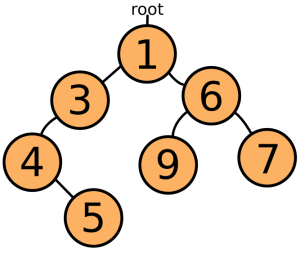
\includegraphics{img/tree.png}
\caption{}
\end{figure}

De telles structures sont appelées des arbres, à cause de la façon dont
elles se séparent en branches. Maintenant, lorsque vous cherchez le plus
petit élément, vous avez juste à prendre l'élément supérieur et
réarranger l'arbre pour que l'un des fils de cet élement supérieur --
celui avec la plus petite valeur devienne le nouvel élément supérieur.
Lorsque vous insérez de nouveaux éléments, vous `descendez' l'arbre
jusqu'à ce que vous trouviez un élément plus petit que ce nouvel
élément, et vous l'insérez à cet endroit. Cela nécessite beaucoup moins
de recherches que dans un tableau trié, mais cela a l'inconvénient de
créer beaucoup d'objets, ce qui ralentit aussi les choses.

\begin{center}\ding{67}\end{center}

Un tas binaire, lui, utilise un tableau trié, mais il n'est que
partiellement trié, un peu comme l'arbre ci-dessus. Au lieu d'objets,
les positions dans le tableau sont utilisées pour former l'arbre, comme
ce qu'essaie de montrer cette image :

\begin{figure}[ht!]
\centering
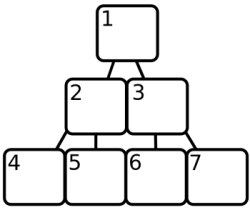
\includegraphics{img/heap.png}
\caption{}
\end{figure}

L'élément \texttt{1} du tableau est la racine de l'arbre, les éléments
\texttt{2} et \texttt{3} sont ses fils, et d'une façon générale,
l'élément \texttt{X} du tableau a comme fils les élements \texttt{X * 2}
et \texttt{X * 2 + 1}. Vous pouvez voir pourquoi cette structure est
appelée `tas' . Remarquez que ce tableau commence à \texttt{1} alors que
les tableaux JavaScript commence à \texttt{0}. Le tas conserve toujours
son plus petit élément en \texttt{1}, et s'assure que pour tout élément
du tableau à la position \texttt{X}, l'élément \texttt{X/2} (arrondi à
l'inférieur) est plus petit.

Pour trouver désormais le plus petit élément, il faut prendre l'élément
à la position \texttt{1}. Mais quand cet élément est supprimé, le tas
doit s'assurer qu'il ne reste pas de trous dans le tableau. Pour cela,
il prend le dernier élément du tableau, et le remonte au départ. Il le
compare ensuite avec ses éléments fils aux positions \texttt{2} et
\texttt{3}. Il est probable qu'ils seront plus grands, on l'échange donc
avec l'un d'entre eux, et le processus de comparaison avec ses fils est
répété pour la nouvelle position, et ainsi de suite, jusqu'à arriver à
une position où ses fils sont plus grands, ou à une position où il n'a
pas de fils.

\begin{lstlisting}
[2, 3, 5, 4, 8, 7, 6]
On enlève 2, on déplace 6 au début.
[6, 3, 5, 4, 8, 7]
6 est plus grand que son premier fils 3, donc on les échange.
[3, 6, 5, 4, 8, 7]
Maintenant 6 a pour fils 4 et 8 (position 4 et 5). Il est plus grand que
4, donc on les échange de nouveau.
[3, 4, 5, 6, 8, 7]
6 est en position 4, et n'a plus de fils. Le tas est de nouveau trié.
\end{lstlisting}
De la même façon, lorsqu'un élément est ajouté au tas, on le met à la
fin du tableau et on l'autorise à `remonter' (comme une bulle de savon)
en l'échangeant de façon répétée avec son parent, jusqu'à ce que l'on
trouve un parent qui est plus petit que le nouvel élément.

\begin{lstlisting}
[3, 4, 5, 6, 8, 7]
On joute l'élément 2 de nouveau, il démarre à la fin.
[3, 4, 5, 6, 8, 7, 2]
2 est en position 7, son parent est en position 3, où se trouve un 5.
5 est plus grand que 2, donc on les échange.
[3, 4, 2, 6, 8, 7, 5]
Le parent de la position 3 est la position 1. De nouveau, on échange.
[2, 4, 3, 6, 8, 7, 5]
L'élément ne peut pas aller plus loin que la position 1, on a donc fini.
\end{lstlisting}
Remarquez comment l'ajout et la suppression d'un élément ne nécessitent plus de le comparer à tous les éléments du tableau. En fait, comme les sauts entre parents et enfants deviennent de plus en plus grands à mesure que le tableau grandit, cet avantage est particulièrement important lorsque vous avez de nombreux éléments\footnote{Le nombre de comparaisons et d'échanges nécessaires, dans le pire des cas, peut être estimé en prenant le logarithme (base 2) du nombre  d'éléments du tas.}.

\begin{center}\ding{67}\end{center}

Voici le code complet de l'implémentation du tas binaire. Deux choses
sont à noter. Premièrement, au lieu de comparer directement les éléments
mis dans le tas, une fonction (\texttt{fonctionScore}) est appliquée en
premier lieu, ce qui permet de stocker des éléments qui ne peuvent pas
être comparés directement.

Deuxièmement, comme les tableaux JavaScript commencent en \texttt{0}, et
que les calculs parents/fils utilisent un système qui démarre en
\texttt{1}, il y a quelques calculs bizarres pour compenser cette
différence.

\begin{lstlisting}
function BinaryHeap(fonctionScore){
  this.contenu = [];
  this.fonctionScore = fonctionScore;
}

BinaryHeap.prototype = {
  push: function(element) {
    // Ajouter le nouvel élément à la fin du tableau.
    this.contenu.push(element);
    // L'autoriser à remonter.
    this.bubbleUp(this.contenu.length - 1);
  },

  pop: function() {
    // Stocker le premier élément, pour pouvoir le renvoyer plus tard
    var resultat = this.contenu[0];
    // Récupérer l'élément à la fin du tableau.
    var fin = this.contenu.pop();
    // S'il reste au moins un élément,
    // mettre le dernier élément au début et le faire descendre
    if (this.contenu.length > 0) {
      this.contenu[0] = fin;
      this.sinkDown(0);
    }
    return resultat;
  },

  remove: function(noeud) {
    var longueur = this.contenu.length;
    // Pour supprimer une valeur,
    // nous devons parcourir le tableau pour la trouver
    for (var i = 0; i < longueur; i++) {
      if (this.contenu[i] == noeud) {
        // Comme on l'a trouvé, on répéte le processus vu dans 'pop'
        // pour boucher le trou
        var end = this.contenu.pop();
        if (i != longueur - 1) {
          this.contenu[i] = end;
          if (this.fonctionScore(end) < this.fonctionScore(noeud))
            this.bubbleUp(i);
          else
            this.sinkDown(i);
        }
        return;
      }
    }
    throw new Error("Noeud non trouvé.");
  },

  size: function() {
    return this.contenu.length;
  },

  bubbleUp: function(n) {
    // On va chercher l'élément qui doit être déplacé
    var element = this.contenu[n];
    // Quand il est à 0, un élément ne peut pas remonter plus haut
    while (n > 0) {
      // Calculer l'index du parent de l'élément, et aller le chercher.
      var parentN = Math.floor((n + 1) / 2) - 1,
          parent = this.contenu[parentN];
      // Echanger les éléments si le parent est plus grand.
      if (this.fonctionScore(element) < this.fonctionScore(parent)) {
        this.contenu[parentN] = element;
        this.contenu[n] = parent;
        // Mettre à jour 'n' pour continuer à la nouvelle position.
        n = parentN;
      }
      // On a trouvé un parent qui est plus petit,
      // ce n'est pas nécessaire de le faire bouger davantage.
      else {
        break;
      }
    }
  },

  sinkDown: function(n) {
    // Récupérer l'élément cible et son score.
    var longueur = this.contenu.length,
        element = this.contenu[n],
        scoreElement = this.fonctionScore(element);

    while(true) {
      // Calculer les indices des éléments fils.
      var fils2N = (n + 1) * 2, fils1N = fils2N - 1;
      // On utilise cela pour stocker la nouvelle position de l'élément,
      // s'il y en a une.
      var aEchanger = null;
      // Si le premier fils existe (est à l'intérieur du tableau)...
      if (fils1N < longueur) {
        // On le récupère et on calcule son score.
        var fils1 = this.contenu[fils1N],
            scoreFils1 = this.fonctionScore(fils1);
        // Si le score est plus petit que celui de notre élément, on doit échanger
        if (scoreFils1 < scoreElement)
          aEchanger = fils1N;
      }
      // Faire les mêmes vérifications pour l'autre fils.
      if (fils2N < longueur) {
        var fils2 = this.contenu[fils2N],
            scoreFils2 = this.fonctionScore(fils2);
        if (scoreFils2 < (aEchanger == null ? scoreElement : scoreFils1))
          aEchanger = fils2N;
      }

      // Si l'élément doit être déplacé, on échange et on continue.
      if (aEchanger != null) {
        this.contenu[n] = this.contenu[aEchanger];
        this.contenu[aEchanger] = element;
        n = aEchanger;
      }
      // Sinon, on a fini.
      else {
        break;
      }
    }
  }
};
\end{lstlisting}
Et un test simple\ldots{}

\begin{lstlisting}
var heap = new BinaryHeap(function(x){return x;});
forEach([10, 3, 4, 8, 2, 9, 7, 1, 2, 6, 5],
        method(heap, "push"));

heap.remove(2);
while (heap.size() > 0)
  print(heap.pop());
\end{lstlisting}

© \href{mailto:marijnh@gmail.com}{Marijn Haverbeke} et
\href{contributors.html}{contributeurs}
(\href{http://creativecommons.org/licenses/by/3.0/deed.fr}{licence}),
écrit entre mars et juillet 2007, dernière modification le 28 juin 2012.

                        
                        
% -------------------------------------------------------------------------
%


\appendix
\part*{Annexes}
\addcontentsline{toc}{part}{Annexes}

 
\chapter{Annexe 1}



%
% -------------------------------------------------------------------------

                    

Contenu de l'annexe

%-------------------------------------------------------------------------------

                        
% -------------------------------------------------------------------------
%
%%\appendix%%


\chapter{Glossaire}


%
% -------------------------------------------------------------------------

                    

 Liste descriptive pour un glossaire


%-------------------------------------------------------------------------------

\backmatter

            
                        

\tableofcontents{Table des matières}

\end{document}
